% Options for packages loaded elsewhere
\PassOptionsToPackage{unicode}{hyperref}
\PassOptionsToPackage{hyphens}{url}
%
\documentclass[
]{article}
\usepackage{amsmath,amssymb}
\usepackage{iftex}
\ifPDFTeX
  \usepackage[T1]{fontenc}
  \usepackage[utf8]{inputenc}
  \usepackage{textcomp} % provide euro and other symbols
\else % if luatex or xetex
  \usepackage{unicode-math} % this also loads fontspec
  \defaultfontfeatures{Scale=MatchLowercase}
  \defaultfontfeatures[\rmfamily]{Ligatures=TeX,Scale=1}
\fi
\usepackage{lmodern}
\ifPDFTeX\else
  % xetex/luatex font selection
\fi
% Use upquote if available, for straight quotes in verbatim environments
\IfFileExists{upquote.sty}{\usepackage{upquote}}{}
\IfFileExists{microtype.sty}{% use microtype if available
  \usepackage[]{microtype}
  \UseMicrotypeSet[protrusion]{basicmath} % disable protrusion for tt fonts
}{}
\makeatletter
\@ifundefined{KOMAClassName}{% if non-KOMA class
  \IfFileExists{parskip.sty}{%
    \usepackage{parskip}
  }{% else
    \setlength{\parindent}{0pt}
    \setlength{\parskip}{6pt plus 2pt minus 1pt}}
}{% if KOMA class
  \KOMAoptions{parskip=half}}
\makeatother
\usepackage{xcolor}
\usepackage[margin=1in]{geometry}
\usepackage{color}
\usepackage{fancyvrb}
\newcommand{\VerbBar}{|}
\newcommand{\VERB}{\Verb[commandchars=\\\{\}]}
\DefineVerbatimEnvironment{Highlighting}{Verbatim}{commandchars=\\\{\}}
% Add ',fontsize=\small' for more characters per line
\usepackage{framed}
\definecolor{shadecolor}{RGB}{248,248,248}
\newenvironment{Shaded}{\begin{snugshade}}{\end{snugshade}}
\newcommand{\AlertTok}[1]{\textcolor[rgb]{0.94,0.16,0.16}{#1}}
\newcommand{\AnnotationTok}[1]{\textcolor[rgb]{0.56,0.35,0.01}{\textbf{\textit{#1}}}}
\newcommand{\AttributeTok}[1]{\textcolor[rgb]{0.13,0.29,0.53}{#1}}
\newcommand{\BaseNTok}[1]{\textcolor[rgb]{0.00,0.00,0.81}{#1}}
\newcommand{\BuiltInTok}[1]{#1}
\newcommand{\CharTok}[1]{\textcolor[rgb]{0.31,0.60,0.02}{#1}}
\newcommand{\CommentTok}[1]{\textcolor[rgb]{0.56,0.35,0.01}{\textit{#1}}}
\newcommand{\CommentVarTok}[1]{\textcolor[rgb]{0.56,0.35,0.01}{\textbf{\textit{#1}}}}
\newcommand{\ConstantTok}[1]{\textcolor[rgb]{0.56,0.35,0.01}{#1}}
\newcommand{\ControlFlowTok}[1]{\textcolor[rgb]{0.13,0.29,0.53}{\textbf{#1}}}
\newcommand{\DataTypeTok}[1]{\textcolor[rgb]{0.13,0.29,0.53}{#1}}
\newcommand{\DecValTok}[1]{\textcolor[rgb]{0.00,0.00,0.81}{#1}}
\newcommand{\DocumentationTok}[1]{\textcolor[rgb]{0.56,0.35,0.01}{\textbf{\textit{#1}}}}
\newcommand{\ErrorTok}[1]{\textcolor[rgb]{0.64,0.00,0.00}{\textbf{#1}}}
\newcommand{\ExtensionTok}[1]{#1}
\newcommand{\FloatTok}[1]{\textcolor[rgb]{0.00,0.00,0.81}{#1}}
\newcommand{\FunctionTok}[1]{\textcolor[rgb]{0.13,0.29,0.53}{\textbf{#1}}}
\newcommand{\ImportTok}[1]{#1}
\newcommand{\InformationTok}[1]{\textcolor[rgb]{0.56,0.35,0.01}{\textbf{\textit{#1}}}}
\newcommand{\KeywordTok}[1]{\textcolor[rgb]{0.13,0.29,0.53}{\textbf{#1}}}
\newcommand{\NormalTok}[1]{#1}
\newcommand{\OperatorTok}[1]{\textcolor[rgb]{0.81,0.36,0.00}{\textbf{#1}}}
\newcommand{\OtherTok}[1]{\textcolor[rgb]{0.56,0.35,0.01}{#1}}
\newcommand{\PreprocessorTok}[1]{\textcolor[rgb]{0.56,0.35,0.01}{\textit{#1}}}
\newcommand{\RegionMarkerTok}[1]{#1}
\newcommand{\SpecialCharTok}[1]{\textcolor[rgb]{0.81,0.36,0.00}{\textbf{#1}}}
\newcommand{\SpecialStringTok}[1]{\textcolor[rgb]{0.31,0.60,0.02}{#1}}
\newcommand{\StringTok}[1]{\textcolor[rgb]{0.31,0.60,0.02}{#1}}
\newcommand{\VariableTok}[1]{\textcolor[rgb]{0.00,0.00,0.00}{#1}}
\newcommand{\VerbatimStringTok}[1]{\textcolor[rgb]{0.31,0.60,0.02}{#1}}
\newcommand{\WarningTok}[1]{\textcolor[rgb]{0.56,0.35,0.01}{\textbf{\textit{#1}}}}
\usepackage{longtable,booktabs,array}
\usepackage{calc} % for calculating minipage widths
% Correct order of tables after \paragraph or \subparagraph
\usepackage{etoolbox}
\makeatletter
\patchcmd\longtable{\par}{\if@noskipsec\mbox{}\fi\par}{}{}
\makeatother
% Allow footnotes in longtable head/foot
\IfFileExists{footnotehyper.sty}{\usepackage{footnotehyper}}{\usepackage{footnote}}
\makesavenoteenv{longtable}
\usepackage{graphicx}
\makeatletter
\def\maxwidth{\ifdim\Gin@nat@width>\linewidth\linewidth\else\Gin@nat@width\fi}
\def\maxheight{\ifdim\Gin@nat@height>\textheight\textheight\else\Gin@nat@height\fi}
\makeatother
% Scale images if necessary, so that they will not overflow the page
% margins by default, and it is still possible to overwrite the defaults
% using explicit options in \includegraphics[width, height, ...]{}
\setkeys{Gin}{width=\maxwidth,height=\maxheight,keepaspectratio}
% Set default figure placement to htbp
\makeatletter
\def\fps@figure{htbp}
\makeatother
\setlength{\emergencystretch}{3em} % prevent overfull lines
\providecommand{\tightlist}{%
  \setlength{\itemsep}{0pt}\setlength{\parskip}{0pt}}
\setcounter{secnumdepth}{5}
\usepackage{booktabs}
\ifLuaTeX
  \usepackage{selnolig}  % disable illegal ligatures
\fi
\usepackage[]{natbib}
\bibliographystyle{plainnat}
\usepackage{bookmark}
\IfFileExists{xurl.sty}{\usepackage{xurl}}{} % add URL line breaks if available
\urlstyle{same}
\hypersetup{
  pdftitle={Advanced Geospatial Data Analysis with R -- Applications in Geosciences},
  pdfauthor={Dr.~Marj Tonini, Haokun Liu},
  hidelinks,
  pdfcreator={LaTeX via pandoc}}

\title{Advanced Geospatial Data Analysis with R -- Applications in Geosciences}
\author{Dr.~Marj Tonini, Haokun Liu}
\date{09/12/2024}

\begin{document}
\maketitle

{
\setcounter{tocdepth}{2}
\tableofcontents
}
\section*{Preface}\label{preface}
\addcontentsline{toc}{section}{Preface}

Earth surface environmental processes exhibit distinctive characteristics, encompassing both spatial and temporal dimensions, along with various attributes and predictive variables.
Coupled with uncertainty and complexity issues, all this contributes to make this field of research highly challenging.
Furthermore, in the era of Data Science, the wealth of available data and the rapid development of analytical models have emerged as distinctive aspects in the realm of \textbf{Advanced Geospatial Data Analysis (AGDA)}.
The domain of AGDA encompasses data exploration, manipulation, and modelling, from the acquisition phase up to the visualization and interpretation of the results.
Mapping where events are located and how they relate to each other provides a better understanding of the process being studied.
Finally, as an increasing volume of geo-environmental data becomes more and more accessible, the demand for spatial data scientists is growing rapidly, both in public research institutions as well as in private companies.

The term ``\textbf{Data Science}'' was defined for the first time by Peter Naur in 1974 as ``\emph{the science of dealing with data, once they have been established, while the relation of the data to what they represent is delegated to other fields and sciences}'' \citep{naur_peter_concise_1974}.
In essence, this definition frames Data Science as the technical and methodological handling of data, while their initial creation or gathering, as well as the interpretation of its meaning in the broader context, is not the primary focus of this discipline.
In 1977 the International Association for Statistical Computing (\href{https://iasc-isi.org/}{IASC}) further refined the concept of Data Science, emphasizing its role in the process of transforming raw data into valuable information and actionable knowledge.
The IASC articulated that Data Science involves not only the collection and processing of data, but also the application of statistical methods and computational techniques to extract meaningful insights, which can then be used to support decision-making and drive innovation across various domains.

In disciplines like environmental and earth Sciences, physical geography, humanities and social sciences, the use of Data Science procedures is emerging only recently, proving to be extremely efficient to deal with the complexity of the investigated process and the heterogeneity of the underlying data sources \citep{amato_spatiotemporal_2022}.
This leads to a cultural shift, moving scientists away from individual working within their own research domain.
Indeed, disciplinary boundaries are more and more permeable, pushing scientists to be more open to collaborate among them and with decision makers on the investigation and understanding of real-world problems.
Modern earth and environmental scientists need to interact with other disciplines, apparently far from their domain.
This openness is increasingly important as society struggles to respond to the implication of anthropogenic pressures on different issues, such as natural hazards and climate change, or the harmful impacts of human activities on biodiversity, water and air quality, human health.

\subsection*{Book overview}\label{book-overview}
\addcontentsline{toc}{subsection}{Book overview}

This eBook primarily focuses on introducing analytical techniques from the field of Data Science to analyze and understand environmental processes occurring on Earth's surface.
Mastering the methodologies in this multidisciplinary and rapidly evolving field---encompassing statistics, mathematics, geomatics, and computer science---can be a challenging endeavor.
To address this, the eBook maintains a rigorous foundation in mathematical and statistical principles while emphasizing practical applications within the domain of Geosciences.

Emphasis is placed on the application of advanced geospatial tools to analyze and model both natural and anthropogenic hazards, as well as land-use processes.
Theoretical concepts are reinforced through case studies employing spatial clustering techniques and both supervised and unsupervised machine learning algorithms.
Examples include stochastic point process models for spatio-temporal cluster analysis and machine learning-based approaches for geodemographic segmentation, susceptibility assessment, and risk mapping.

\subsubsection*{Computing lab}\label{computing-lab}
\addcontentsline{toc}{subsubsection}{Computing lab}

Computations are conducted using the R free software environment, which is specifically designed for data analysis and manipulation.

After a brief introduction to the main functionalities in R (see Chapter \ref{intro}) and an overview of the basic operations with geospatial data (see Chapter \ref{geodata}), the rest of the chapters will focus on the following geo-computational techniques:

\begin{itemize}
\tightlist
\item
  \emph{Exploratory Data Analysis and Visualization}: examining geographical variations in statistical data distributions, including Geographically Weighted Summary Statistics (Chapter \ref{gwss}).
\item
  \emph{Cluster Detection and Mapping}: using global clustering methods, namely Ripley's K-function and Kernel Density Estimator (Chapter \ref{kde}).
\item
  \emph{Random Forest}: as example of supervised machine learning algorithm. We present both the global (Chapter \ref{global-rf}) and the local version, and we use Random Forest to introduce interpretability \& explainability in machine learning (Chapter \ref{local-rf}) .
\item
  \emph{Self-Organizing Maps}: as example of unsupervised machine learning method for data clustering/segmentation and visualization (Chapter \ref{som}).
\item
  \emph{Feature detection}: using DBSCAN for identifying and visualizing clustering features (Chapter \ref{dbscan}).
\end{itemize}

To complete the applied computing labs presented in each chapter, readers can download the datasets from here: \href{data}{dataset}

\subsubsection*{Target audience}\label{target-audience}
\addcontentsline{toc}{subsubsection}{Target audience}

The target audience includes master's and PhD students in Earth and Environmental Sciences, Biology and Spatial Ecology, Physical Geography, and related disciplines.
Our goal is to empower students by guiding them through both theoretical knowledge and hands-on practical applications, helping them develop strong problem-solving skills.

\textbf{This eBook aims to equip the audience with}:

\begin{itemize}
\tightlist
\item
  A solid understanding of key practical concepts and applied aspects in AGDA.
\item
  Advanced tools to effectively navigate and analyze spatial datasets in Geosciences.
\end{itemize}

The eBook is designed for intermediate to advanced R users with previous experience in geospatial data analyses and a keen interest in geocomputing.
If you have only a basic knowledge of these areas, we strongly encourage you to explore the essential references provided in each chapter.
These resources offer valuable documentation and additional materials to help deepen your understanding.

\textbf{The main prerequisites are the following}:

\begin{itemize}
\tightlist
\item
  Knowledge of basic statistics: methods of descriptive statistics (measures of central tendency and dispersion); how to assess relationships between variables; concepts of correlation and regression.
\item
  Basic knowledge in geomatics (GIS): basic operations with raster and vector datasets.
\item
  R programming basics and RStudio.
\end{itemize}

\subsection*{Authors information}\label{authors-information}
\addcontentsline{toc}{subsection}{Authors information}

\textbf{Marj Tonini} is a spatial data scientist with a profound expertise in geospatial modeling for risk assessment, particularly in relation to wildfires and landslides.
She earned her Ph.D.~in 2002 from the \href{https://www.santannapisa.it/en}{Sant'Anna School of Advanced Studies} in Pisa, Italy, where she developed a thesis on agro-environmental modeling that laid the foundation for her career.
In 2004, she joined the \href{https://www.unil.ch/central/en/home.html}{University of Lausanne} (UNIL) as a postdoctoral researcher in geospatial data analysis, and by 2008, she was appointed as Senior Research Manager at the \href{https://www.unil.ch/idyst/en/home.html}{Institute of Earth Surface Dynamics}, where she continues to serve in her current role.
Sine 2022 she has been servig a four-year term as the director of the \href{https://unil-sgc.github.io/}{Swiss Geocomputing Centre} of the Faculty of Geosciences and environment (UNIL)

Marj's research focuses on the development of innovative methodologies that facilitate the efficient extraction of knowledge from complex environmental datasets.
Her work aims to estabilishing a robust methodological framework to understand the spatio-temporal dynamics of environmental processes and to evaluate the influence of various predictor variables.
Her current research focuses on the analysis of land use and land cover changes, alongside the development of predictive scenarios and the assessment of susceptibility and risks associated with natural hazards.
Through this work she seeks to advance the field of geospatial science by translating data-driven insights into practical solutions for managing and mitigating environmental risks.
You can find the full list of her publications on \href{https://www.researchgate.net/profile/Marj-Tonini-2}{ResearchGate} and \href{https://scholar.google.it/citations?user=qXexP-IAAAAJ&hl=en}{Google Scholar}.

Marj has written the vast majority of this book.
Her contributions include the development of the conceptual framework, writing the theoretical background chapters, developing case studies, designing methodologies, conducting data collection and analysis, and software/tool development.
The following section ``\emph{My Journey of Learning}'' refers to her personal experience.

\textbf{Haokun Liu} is a Ph.D.~student at the Group of \href{https://wp.unil.ch/citadyne-news/}{Cities and Dynamics of Networks}, \href{https://www.unil.ch/central/en/home.html}{University of Lausanne}.
In addition to his doctoral studies, he serves as a student assistant at the \href{https://unil-sgc.github.io/}{Swiss Geocomputing Center}.
Benefiting from rigorous and comprehensive training in both China and Switzerland, Haokun has developed a diverse research portfolio.
His primary research interests and experience encompass a wide range of interdisciplinary fields, including urban analytics, health geography, and spatial data science.
His work focuses on leveraging advanced computational techniques to address complex urban and environmental challenges, bridging the gap between data-driven insights and real-world applications.

Haokun's contributions were instrumental in establishing and managing the GitHub repository used to host and maintain this eBook.
He also played a key role in data visualization and mapping, and provided valuable revisions to the applied computing labs.

\subsection*{My Journey of Learning: Integrating Geospatial Data Analysis with Data Science}\label{my-journey-of-learning-integrating-geospatial-data-analysis-with-data-science}
\addcontentsline{toc}{subsection}{My Journey of Learning: Integrating Geospatial Data Analysis with Data Science}

In the early 2000s, as I (Marj) embarked on my PhD journey, a new frontier was beginning to unfold in Geosciences.
Geographical information systems (GIS) were just starting to make waves, offering a fresh perspective on how researchers could investigate and understand the environment.
It was through my thesis on the effects of spreading olive vegetation water on agricultural land that I first delved into the world of GIS.
This early exposure was more than just a technical skill; it was a revelation that would drive me to explore the depths of spatial analysis for years to come.

After completing my PhD, my journey led me to a PostDoc position where I had the privile of working with Professor \href{https://www.egu.eu/awards-medals/ian-mcharg/2022/mikhail-kanevski/}{Mikhail Kanevski}, a true pioneer in the fields of environmental data mining, geostatistics, and the emerging field of applying machine learning to spatial environmental data.
In this dynamic research team, I found myself diving headfirst into the world of spatial data science, driven by the desire to uncover valuable insights from the complex data that described our environment.
The work was challenging, yet it was also exhilarating, as every new technique I learned brought me closer to understanding the intricate tapestry of environmental phenomena.

As the years passed, the tools and resources available to researchers like me grew exponentially.
The development and widespread adoption of free programming languages like and \href{https://www.r-project.org/}{R} and \href{https://www.python.org/}{Python} revolutionized the way we approached statistical analysis and machine learning.
What was once the domain of a select few became accessible to many, thanks to the wealth of pre-developed scripts and resources these languages offered.
For me, and for countless others, this accessibility was a game-changer.
It meant that advanced techniques were no longer out of reach, and it fostered a culture of greater reproducibility in research.
By utilizing standardized, widely adopted open-source programming languages and cloud-based platforms for hosting and managing Git repositories, such as \href{https://github.com/}{GitHub}, researchers can now more easily share their code and methodologies, enabling others to replicate and validate their findings.
This collaborative spirit has enhanced the reliability and credibility of scientific research and fostered a community where knowledge is shared and expanded more efficiently.

Reflecting on this journey, I realize that each step -- from my early days with GIS to my current role as an independent lead researcher in environmental spatial data analysis in the era of Data Science -- has been a chapter in a larger story of discovery and innovation.
It's a story of how spatial data and advanced analytics have become indispensable tools in our quest to understand and protect the environment, and it's a story that continues to unfold with each new challenge and breakthrough.

\subsection*{Acknowledgements}\label{acknowledgements}
\addcontentsline{toc}{subsection}{Acknowledgements}

The case studies presented in each chapter came from different projects carried out in collaboration with several colleagues, including master and PhD students.
All the produced scientific papers are duly cited in the bibliography.

I would like to express my gratitude to Professor Mário Gonzalez Pereira and Dr.~Joana Parente, for their extensive and fruitful collaboration in investigating the spatio-temporal distribution of wildfires in Portugal.
One of our studies, which explores the evolution of forest fires from spatio-temporal point events to smoothed density maps, forms an integral part of Chapters 3 and 4.

I also thank Professor Stuart Lane and Dr.~Natan Micheletti for introducing me to the fascinating world of rock glacier research.
Notably, the 3D point cloud dataset analyzed in Chapter 8 was acquired and processed by Natan during his PhD studies.

My thanks also go to Julien Riese, who produced the input dataset and collaborated with me in developing the code that assesses landslide susceptibility in Canton Vaud, the main focus of Chapter 5.
The same for Axelle Bersier for her meticulous work in acquiring and pre-processing the Swiss national population census dataset, which is used for the exercise on unsupervised learning in Chapter 7.
Both Julien and Axelle exemplify the high caliber of master's students I have had the pleasure of supervising.

For transparency, I acknowledge the use of ChatGPT in assisting with the reformulation of certain sentences in this book and DALL-E to generate the image icon.

\section{Introduction to R}\label{intro}

\subsection{R Language}\label{r-language}

R is a complete programming language and software environment for statistical computing and graphical representation.
As part of the GNU Project -- free software, mass collaboration project -- (\url{https://www.gnu.org/software/software.en.html}), the source code is freely available.

For more details on R see \url{https://www.r-project.org/}.

\subsubsection{R Packages}\label{r-packages}

Functionalities in R can be expanded by importing packages.
A package is a collection of R functions, data and compiled code.
The location where the packages are stored is called the ``library''.
If there is a particular functionality that you require, you can download the package from the appropriate site and it will be stored in your library.

In all operation systems the function \texttt{install.packages()} can be used to download and install a package automatically.
Otherwise, a package already installed in R can be loaded in a session by using the command \texttt{library(package\_name)}.
When you open an \hyperref[r-markdown]{R Markdown} document (\emph{.Rmd}) the program propose you automatically to install the libraries listed there.

\subsubsection{Some tips}\label{some-tips}

\begin{itemize}
\tightlist
\item
  R is case sensitive!
\item
  Previously used command can be recalled in the console by using the up arrow on the keyboard.
\item
  The working directory by default is ``\texttt{C:/user/.../Documents}''.

  \begin{itemize}
  \tightlist
  \item
    It can be found using the command \texttt{getwd()}
  \item
    It can be changed using the command line \texttt{setwd("C:/Your/own/path")}
  \end{itemize}
\item
  In R Markdown the working directory when evaluating R code chunks is the directory of the input document by default.

  \begin{itemize}
  \tightlist
  \item
    To access to a specific file in a sub-folder use ``\texttt{.\ /subfolder/file.ext}''
  \item
    To access to a specific file in a up-folder use ``\texttt{.\ .\ /upfolder/file.ext}''
  \end{itemize}
\end{itemize}

\subsubsection{R Commands (online resources)}\label{r-commands-online-resources}

Many table resuming the main R commands can be found online.\\
Here some useful links:

\begin{itemize}
\tightlist
\item
  \href{https://www.maths.usyd.edu.au/u/jchan/Rcommands.pdf}{A short list of the most useful R commands}
\item
  \href{https://sites.calvin.edu/scofield/courses/m143/materials/RcmdsFromClass.pdf}{Table of Useful R commands}
\item
  \href{https://rpubs.com/ssammut/ResearchStats}{Basic Commands to Get Started with R}
\end{itemize}

\subsection{R Markdown}\label{r-markdown}

This is an R Markdown document :-)

Markdown is a simple formatting syntax for authoring HTML, PDF, and MS Word documents.
It is a simple and easy to use plain text language allowing to combine R code, results from data analysis (including plots and tables), and comments into a single nicely formatted and reproducible document like a report, publication, thesis chapter or web pages.

Code lines are organized into code blocks, seeking to solve specified tasks, and referred to as ``code chunk''.
For more details on using R Markdown see \url{http://rmarkdown.rstudio.com}.

All what you have to do during the computing labs is to read each explanatory paragraph before running each individual R code chunk, one by one, and to interpret the results.
Finally, to create a personal document (usually a PDF) from R Markdown, you need to \emph{Knit} the document.
Knitting a document simply means taking all the text and code and creating a nicely formatted document.

\subsection{Data type in computational analysis}\label{data-type-in-computational-analysis}

\subsubsection{Variables}\label{variables}

Variables are used to store values in a computer program.
Values can be numbers (real and complex), words (string), matrices, and even tables.

The fundamental or atomic data in R Programming can be:

\begin{itemize}
\tightlist
\item
  \textbf{integer}: number without decimals
\item
  \textbf{numeric}: number with decimals (\emph{float} or \emph{double} depending on the precision)
\item
  \textbf{character}: string, label
\item
  \textbf{factors}: a label with a limited number of categories
\item
  \textbf{logical}: true/false
\end{itemize}

\begin{figure}

{\centering 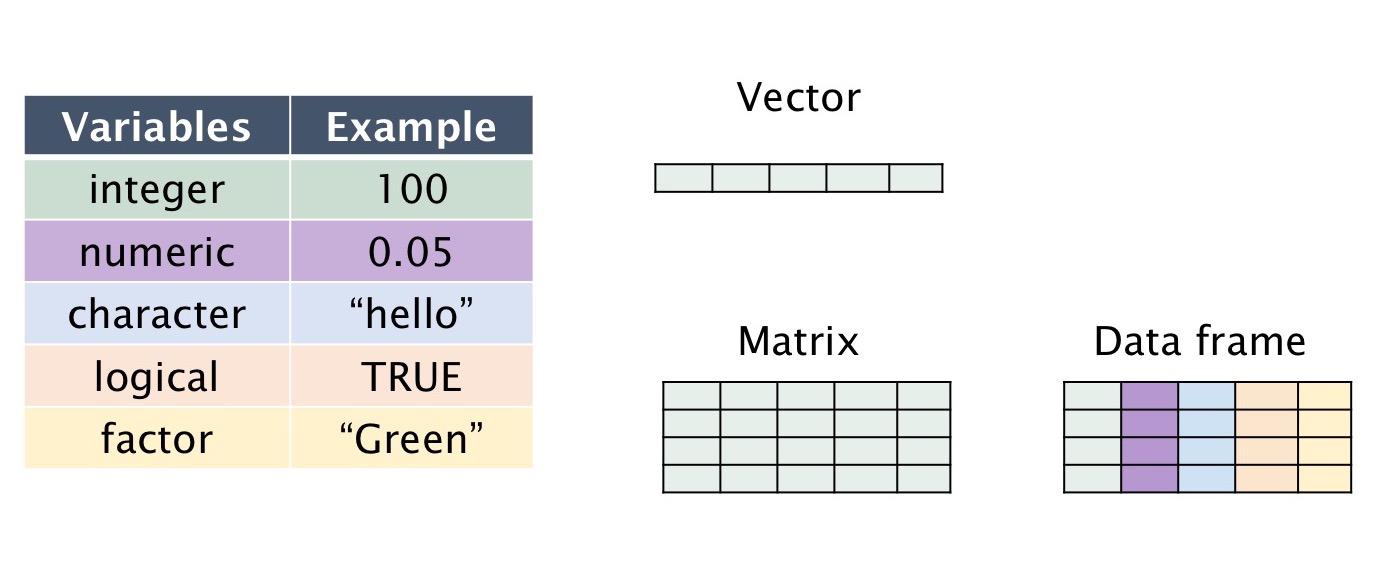
\includegraphics[width=1\linewidth,height=0.8\textheight]{images/Rvariablesdata} 

}

\caption{Data Types in R \label{data_Type}}\label{fig:img1}
\end{figure}

\subsubsection{Data structure in R}\label{data-structure-in-r}

R's base data structures can be organised by their dimensionality (1d, 2d, or nd) and whether they are homogeneous (all contents must be of the same type) or heterogeneous (the contents can be of different types).
This gives rise to the four data structures most often used in data analysis:

\begin{figure}

{\centering 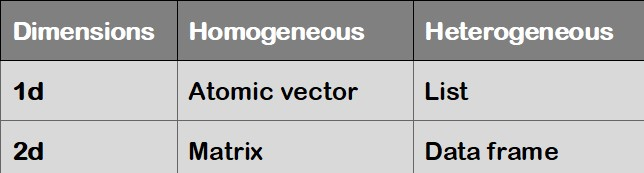
\includegraphics[width=0.5\linewidth,height=0.6\textheight]{images/data_type} 

}

\caption{Data structures in R \label{data_str}}\label{fig:img2}
\end{figure}

A \textbf{Vector} is a one-dimensional structure winch can contain object of one type only: numerical (integer and double), character, and logical.

\begin{Shaded}
\begin{Highlighting}[]
\CommentTok{\# Investigate vector\textquotesingle{}s types:}

\NormalTok{v1 }\OtherTok{\textless{}{-}} \FunctionTok{c}\NormalTok{(}\FloatTok{0.5}\NormalTok{, }\FloatTok{0.7}\NormalTok{); v1; }\FunctionTok{typeof}\NormalTok{(v1)}
\end{Highlighting}
\end{Shaded}

\begin{verbatim}
## [1] 0.5 0.7
\end{verbatim}

\begin{verbatim}
## [1] "double"
\end{verbatim}

\begin{Shaded}
\begin{Highlighting}[]
\NormalTok{v2 }\OtherTok{\textless{}{-}}\FunctionTok{c}\NormalTok{(}\DecValTok{1}\SpecialCharTok{:}\DecValTok{10}\NormalTok{); v2; }\FunctionTok{typeof}\NormalTok{(v2)}
\end{Highlighting}
\end{Shaded}

\begin{verbatim}
##  [1]  1  2  3  4  5  6  7  8  9 10
\end{verbatim}

\begin{verbatim}
## [1] "integer"
\end{verbatim}

\begin{Shaded}
\begin{Highlighting}[]
\NormalTok{v3 }\OtherTok{\textless{}{-}} \FunctionTok{c}\NormalTok{(}\ConstantTok{TRUE}\NormalTok{, }\ConstantTok{FALSE}\NormalTok{); v3; }\FunctionTok{typeof}\NormalTok{(v3)}
\end{Highlighting}
\end{Shaded}

\begin{verbatim}
## [1]  TRUE FALSE
\end{verbatim}

\begin{verbatim}
## [1] "logical"
\end{verbatim}

\begin{Shaded}
\begin{Highlighting}[]
\NormalTok{v4 }\OtherTok{\textless{}{-}} \FunctionTok{c}\NormalTok{(}\StringTok{"Swiss"}\NormalTok{, }\StringTok{"Itay"}\NormalTok{, }\StringTok{"France"}\NormalTok{, }\StringTok{"Germany"}\NormalTok{); v4; }\FunctionTok{typeof}\NormalTok{(v4)}
\end{Highlighting}
\end{Shaded}

\begin{verbatim}
## [1] "Swiss"   "Itay"    "France"  "Germany"
\end{verbatim}

\begin{verbatim}
## [1] "character"
\end{verbatim}

\begin{Shaded}
\begin{Highlighting}[]
\CommentTok{\#Create a sequence from 0 to 5 with a step of 0.5:}

\NormalTok{v5 }\OtherTok{\textless{}{-}} \FunctionTok{seq}\NormalTok{(}\DecValTok{1}\NormalTok{, }\DecValTok{5}\NormalTok{, }\AttributeTok{by=}\FloatTok{0.5}\NormalTok{); v5; }\FunctionTok{typeof}\NormalTok{(v5)}
\end{Highlighting}
\end{Shaded}

\begin{verbatim}
## [1] 1.0 1.5 2.0 2.5 3.0 3.5 4.0 4.5 5.0
\end{verbatim}

\begin{verbatim}
## [1] "double"
\end{verbatim}

\begin{Shaded}
\begin{Highlighting}[]
\FunctionTok{length}\NormalTok{(v5)}
\end{Highlighting}
\end{Shaded}

\begin{verbatim}
## [1] 9
\end{verbatim}

\begin{Shaded}
\begin{Highlighting}[]
\FunctionTok{summary}\NormalTok{(v5)}
\end{Highlighting}
\end{Shaded}

\begin{verbatim}
##    Min. 1st Qu.  Median    Mean 3rd Qu.    Max. 
##       1       2       3       3       4       5
\end{verbatim}

\begin{Shaded}
\begin{Highlighting}[]
\CommentTok{\#Extract the third element of the vector}
\NormalTok{v5[}\DecValTok{3}\NormalTok{]}
\end{Highlighting}
\end{Shaded}

\begin{verbatim}
## [1] 2
\end{verbatim}

\begin{Shaded}
\begin{Highlighting}[]
\CommentTok{\#Exclude the third element from the vector and save as new vector}
\NormalTok{v5[}\SpecialCharTok{{-}}\DecValTok{3}\NormalTok{]}
\end{Highlighting}
\end{Shaded}

\begin{verbatim}
## [1] 1.0 1.5 2.5 3.0 3.5 4.0 4.5 5.0
\end{verbatim}

\begin{Shaded}
\begin{Highlighting}[]
\NormalTok{w5}\OtherTok{\textless{}{-}}\NormalTok{v5[}\SpecialCharTok{{-}}\DecValTok{3}\NormalTok{]; w5}
\end{Highlighting}
\end{Shaded}

\begin{verbatim}
## [1] 1.0 1.5 2.5 3.0 3.5 4.0 4.5 5.0
\end{verbatim}

A \textbf{Matrix} is a two-dimensional structure winch can contain object of one type only.
The function \texttt{matrix()} can be used to construct matrices with specific dimensions.

\begin{Shaded}
\begin{Highlighting}[]
\CommentTok{\# Matrix of elements equal to "zero" and dimension 2x5 }
\NormalTok{m1}\OtherTok{\textless{}{-}}\FunctionTok{matrix}\NormalTok{(}\DecValTok{0}\NormalTok{,}\DecValTok{2}\NormalTok{,}\DecValTok{5}\NormalTok{); m1  }\CommentTok{\#(two rows by five columns)}
\end{Highlighting}
\end{Shaded}

\begin{verbatim}
##      [,1] [,2] [,3] [,4] [,5]
## [1,]    0    0    0    0    0
## [2,]    0    0    0    0    0
\end{verbatim}

\begin{Shaded}
\begin{Highlighting}[]
\CommentTok{\# Matrix of integer elements (1 to 12, 3x4) }
\NormalTok{m2}\OtherTok{\textless{}{-}}\FunctionTok{matrix}\NormalTok{(}\DecValTok{1}\SpecialCharTok{:}\DecValTok{12}\NormalTok{, }\DecValTok{3}\NormalTok{,}\DecValTok{4}\NormalTok{); m2 }
\end{Highlighting}
\end{Shaded}

\begin{verbatim}
##      [,1] [,2] [,3] [,4]
## [1,]    1    4    7   10
## [2,]    2    5    8   11
## [3,]    3    6    9   12
\end{verbatim}

\begin{Shaded}
\begin{Highlighting}[]
\CommentTok{\# Extract the second row}
\NormalTok{m2[}\DecValTok{2}\NormalTok{, ]}
\end{Highlighting}
\end{Shaded}

\begin{verbatim}
## [1]  2  5  8 11
\end{verbatim}

\begin{Shaded}
\begin{Highlighting}[]
\CommentTok{\# Extract the third column}
\NormalTok{m2[,}\DecValTok{3}\NormalTok{]}
\end{Highlighting}
\end{Shaded}

\begin{verbatim}
## [1] 7 8 9
\end{verbatim}

\begin{Shaded}
\begin{Highlighting}[]
\CommentTok{\# Extract the the second element of the third column}
\NormalTok{m2[}\DecValTok{2}\NormalTok{,}\DecValTok{3}\NormalTok{]}
\end{Highlighting}
\end{Shaded}

\begin{verbatim}
## [1] 8
\end{verbatim}

A \textbf{data frame} allows to collect heterogeneous data.
All elements must have the same length.

A \textbf{list} is a more flexible structure since it can contain variables of different types and lengths.
Nevertheless, the preferred structure for statistical analyses and computation is the data frame.

It is a good practice to explore the data frame before performing further computation on the data.
This can be simply accomplished by using the commands \texttt{str()} to explore the structure of the data and \texttt{summary()} to display the summary statistics and quickly summarize the data.
For numerical vectors the command \texttt{hist()} can be used to plot the basic histogram of the given values.

\begin{Shaded}
\begin{Highlighting}[]
\CommentTok{\# Create the vectors with the variables}
\NormalTok{cities }\OtherTok{\textless{}{-}} \FunctionTok{c}\NormalTok{(}\StringTok{"Berlin"}\NormalTok{, }\StringTok{"New York"}\NormalTok{, }\StringTok{"Paris"}\NormalTok{, }\StringTok{"Tokyo"}\NormalTok{)}
\NormalTok{area }\OtherTok{\textless{}{-}} \FunctionTok{c}\NormalTok{(}\DecValTok{892}\NormalTok{, }\DecValTok{1214}\NormalTok{, }\DecValTok{105}\NormalTok{, }\DecValTok{2188}\NormalTok{)}
\NormalTok{population }\OtherTok{\textless{}{-}} \FunctionTok{c}\NormalTok{(}\FloatTok{3.4}\NormalTok{, }\FloatTok{8.1}\NormalTok{, }\FloatTok{2.1}\NormalTok{, }\FloatTok{12.9}\NormalTok{)}
\NormalTok{continent }\OtherTok{\textless{}{-}} \FunctionTok{c}\NormalTok{(}\StringTok{"Europe"}\NormalTok{, }\StringTok{"Norh America"}\NormalTok{, }\StringTok{"Europe"}\NormalTok{, }\StringTok{"Asia"}\NormalTok{)}
\end{Highlighting}
\end{Shaded}

\begin{Shaded}
\begin{Highlighting}[]
\CommentTok{\# Concatenate the vectors into a new data frame}
\NormalTok{df1 }\OtherTok{\textless{}{-}} \FunctionTok{data.frame}\NormalTok{(cities, area, population, continent)}
\NormalTok{df1}
\end{Highlighting}
\end{Shaded}

\begin{verbatim}
##     cities area population    continent
## 1   Berlin  892        3.4       Europe
## 2 New York 1214        8.1 Norh America
## 3    Paris  105        2.1       Europe
## 4    Tokyo 2188       12.9         Asia
\end{verbatim}

\begin{Shaded}
\begin{Highlighting}[]
\CommentTok{\#Add a column (e.g., language spoken) using the command "cbind"}
\NormalTok{df2 }\OtherTok{\textless{}{-}} \FunctionTok{cbind}\NormalTok{ (df1, }\StringTok{"Language"} \OtherTok{=} \FunctionTok{c}\NormalTok{ (}\StringTok{"German"}\NormalTok{, }\StringTok{"English"}\NormalTok{, }\StringTok{"Freanch"}\NormalTok{, }\StringTok{"Japanese"}\NormalTok{))}
\NormalTok{df2}
\end{Highlighting}
\end{Shaded}

\begin{verbatim}
##     cities area population    continent Language
## 1   Berlin  892        3.4       Europe   German
## 2 New York 1214        8.1 Norh America  English
## 3    Paris  105        2.1       Europe  Freanch
## 4    Tokyo 2188       12.9         Asia Japanese
\end{verbatim}

\begin{Shaded}
\begin{Highlighting}[]
\CommentTok{\#Explore the data frame}
\FunctionTok{str}\NormalTok{(df2) }\CommentTok{\# see the structure}
\end{Highlighting}
\end{Shaded}

\begin{verbatim}
## 'data.frame':    4 obs. of  5 variables:
##  $ cities    : chr  "Berlin" "New York" "Paris" "Tokyo"
##  $ area      : num  892 1214 105 2188
##  $ population: num  3.4 8.1 2.1 12.9
##  $ continent : chr  "Europe" "Norh America" "Europe" "Asia"
##  $ Language  : chr  "German" "English" "Freanch" "Japanese"
\end{verbatim}

\begin{Shaded}
\begin{Highlighting}[]
\FunctionTok{summary}\NormalTok{(df2) }\CommentTok{\# compute basic statistics}
\end{Highlighting}
\end{Shaded}

\begin{verbatim}
##     cities               area          population      continent        
##  Length:4           Min.   : 105.0   Min.   : 2.100   Length:4          
##  Class :character   1st Qu.: 695.2   1st Qu.: 3.075   Class :character  
##  Mode  :character   Median :1053.0   Median : 5.750   Mode  :character  
##                     Mean   :1099.8   Mean   : 6.625                     
##                     3rd Qu.:1457.5   3rd Qu.: 9.300                     
##                     Max.   :2188.0   Max.   :12.900                     
##    Language        
##  Length:4          
##  Class :character  
##  Mode  :character  
##                    
##                    
## 
\end{verbatim}

\begin{Shaded}
\begin{Highlighting}[]
\CommentTok{\# Use the symbol "$" to address a particular column}
\NormalTok{pop}\OtherTok{\textless{}{-}}\NormalTok{(df2}\SpecialCharTok{$}\NormalTok{population)}
\NormalTok{pop}
\end{Highlighting}
\end{Shaded}

\begin{verbatim}
## [1]  3.4  8.1  2.1 12.9
\end{verbatim}

\begin{Shaded}
\begin{Highlighting}[]
\FunctionTok{hist}\NormalTok{(pop) }\CommentTok{\# plot the histogram}
\end{Highlighting}
\end{Shaded}

\begin{center}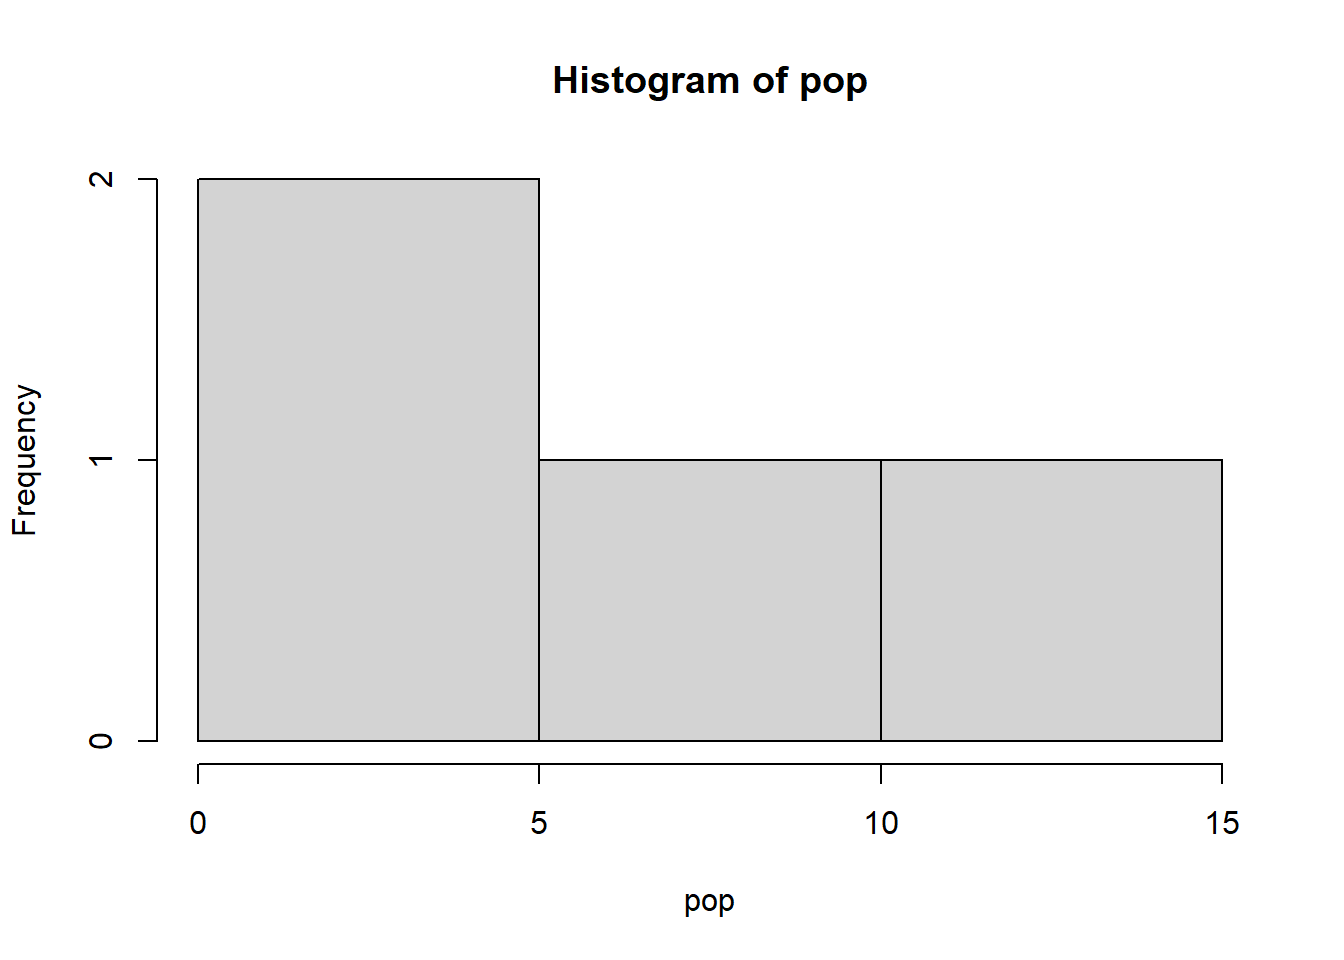
\includegraphics{01-IntrotoR_files/figure-latex/data-exp-1} \end{center}

\section{Basic operations with geodata in R}\label{geodata}

\subsection{Introduction}\label{introduction}

Geodata, or geospatial data, refers to features associated with a specific location on the Earth's surface. Geodata can be in various forms and is often used in Geographic Information Systems (GIS) for mapping and analysis. The two key components characterizing geodata are the \textbf{spatial component} and \textbf{attributes}. The spatial component specifies the location and shape of the features, with different levels of detail, while attributes describe their characteristics.

The two basic formats used to represent the spatial component of geodata are:

\begin{enumerate}
\def\labelenumi{\arabic{enumi}.}
\tightlist
\item
  \textbf{Vector}: this format uses points, lines, and polygons to identify each individual features.
\item
  \textbf{Raster}: this format uses a regular grid of pixels to represent the global geographic context.
\end{enumerate}

In addition, \textbf{attribute tables} are used to store the characteristics associated with the geospatial features.

The GIS software are specifically designed to help user to edit, manage, analyze, and map geodata. To make working with geodata easier, several packages have been developed in R. These packages allow users to handle geodata directly in R computing environment, without needing separate GIS software.

In this chapter, we introduce the basic functions allowing to work with geodata in the pre-processing and post-processing phase of a pipeline in geomodeling.

\subsection{Plotting vector dataset}\label{plotting-vector-dataset}

The spatial component of geodata uses geometric primitives like point, line, and polygon to represent the single features. Each feature in a geodataset is associated with various attributes providing detailed quantitative and qualitative information. A single geodataset includes features of the same type, represented by using the same class of primitive.

The three basic \textbf{geometric vector primitives} have the following characteristics:

\begin{itemize}
\tightlist
\item
  \emph{Points}: defined by a single pair of coordinates (x, y) representing a specific location. Used to represent small objects like weather stations, city center, or to identify single features in a geo-hazard inventory (e.g., earthquake's epicenter, landslides location, wildfires, etc.).
\item
  \emph{Lines}: defined by pairs of coordinates connected to each other, representing linear features such as roads or rivers network, pathways, railway, etc.
\item
  \emph{Polygons}: defined by a series of connected coordinates that enclose an area, representing features such as lakes, administrative units, vegetation patches, burned area, landslides footprint.
\end{itemize}

\subsubsection{\texorpdfstring{Package \textbf{\emph{sf}} for vector dataset}{Package sf for vector dataset}}\label{package-sf-for-vector-dataset}

The package \textbf{sf} \citep{Pebesma_2023, Pebesma_2018} has been designed to work with vector data as ``simple features'' in R. Each feature is represented by one row in the data frame, with attributes stored as columns and spatial information stored in a special geometry column.

\begin{Shaded}
\begin{Highlighting}[]
\CommentTok{\# Load the library sf }
\FunctionTok{library}\NormalTok{(sf)}
\end{Highlighting}
\end{Shaded}

As a toy example, we will work with the geodataset of administrative boundaries in the Canton of Vaud (Switzerland). This dataset is available in shapefile format, one of the most widely used file formats for vector geospatial data. The field ``Munics'' represents the municipalities.

A \textbf{shapefile} includes multiple files allowing to store different kind of objects:

\begin{itemize}
\tightlist
\item
  \emph{*shp}: the features' geometries (i.e., the geometric vector primitive used to describe the features).
\item
  \emph{*dbf}: the attributes, describing the characteristics of the features (i.e., tabular information).
\item
  \emph{*shx}: shape index format, an index file for the geometry data.
\item
  \emph{*prj}: the coordinate reference systems, defining how the geometries are projected on the Earth's surface.
\end{itemize}

To read a shapefile, you only need to specify the file name with ``.shp'' extension. However, it is important to have all related files in the same directory to ensures that the shapefile is read correctly and all necessary information is available for the analysis.

Shapefiles can be imported and converted as sf-objects using the command \texttt{st\_read()}. By setting the argument \texttt{quiet\ =\ FALSE} suppresses the output from the console when importing geodata.

\begin{Shaded}
\begin{Highlighting}[]
\CommentTok{\# Load dataset}
\NormalTok{vaud }\OtherTok{\textless{}{-}} \FunctionTok{st\_read}\NormalTok{(}\StringTok{"data/RGIS/Vaud.shp"}\NormalTok{, }\AttributeTok{quiet =} \ConstantTok{FALSE}\NormalTok{)}
\end{Highlighting}
\end{Shaded}

\begin{verbatim}
## Reading layer `Vaud' from data source `C:\AGDA_Rbook\data\RGIS\Vaud.shp' using driver `ESRI Shapefile'
## Simple feature collection with 315 features and 4 fields
## Geometry type: POLYGON
## Dimension:     XY
## Bounding box:  xmin: 2494306 ymin: 1115149 xmax: 2585462 ymax: 1203493
## Projected CRS: CH1903+ / LV95
\end{verbatim}

\begin{Shaded}
\begin{Highlighting}[]
\CommentTok{\# Inspect the attribute table }
\FunctionTok{str}\NormalTok{(vaud)}
\end{Highlighting}
\end{Shaded}

\begin{verbatim}
## Classes 'sf' and 'data.frame':   315 obs. of  5 variables:
##  $ Shape_Leng: num  30547 21405 27147 31111 28268 ...
##  $ Shape_Area: num  24178457 23354685 23190781 22858943 22501915 ...
##  $ Munics    : chr  "Payerne" "Rossinière" "Vallorbe" "Puidoux" ...
##  $ Code      : chr  "5822" "5842" "5764" "5607" ...
##  $ geometry  :sfc_POLYGON of length 315; first list element: List of 1
##   ..$ : num [1:783, 1:2] 2559434 2559258 2559286 2559263 2559337 ...
##   ..- attr(*, "class")= chr [1:3] "XY" "POLYGON" "sfg"
##  - attr(*, "sf_column")= chr "geometry"
##  - attr(*, "agr")= Factor w/ 3 levels "constant","aggregate",..: NA NA NA NA
##   ..- attr(*, "names")= chr [1:4] "Shape_Leng" "Shape_Area" "Munics" "Code"
\end{verbatim}

\subsubsection{Plot vector features}\label{plot-vector-features}

Basic maps can be created with the command \texttt{plot()}. By default this creates a multi-panel plot: one plot for each variable included in the geodata (corresponding to each column). Otherwise, you can specify the name of variable that you wish to display.

\begin{Shaded}
\begin{Highlighting}[]
\CommentTok{\# Basic plot (diplay all the variables)}
\FunctionTok{plot}\NormalTok{(vaud) }
\end{Highlighting}
\end{Shaded}

\begin{center}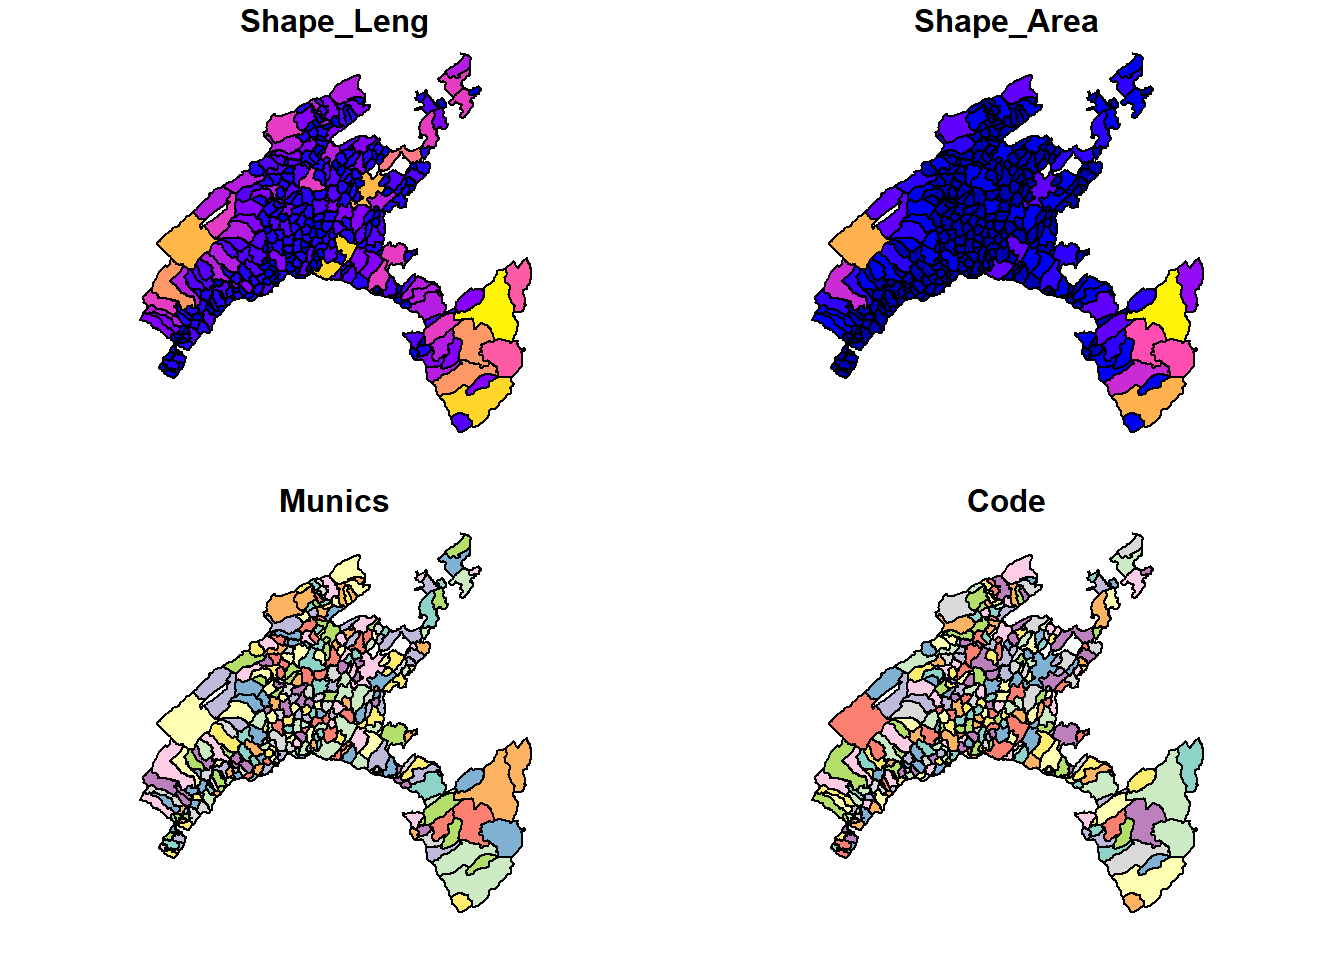
\includegraphics{02-RGIS_files/figure-latex/simple-plot-1} \end{center}

\begin{Shaded}
\begin{Highlighting}[]
\CommentTok{\# Display each municipality using single color (attributed randomly)}
\FunctionTok{plot}\NormalTok{(vaud[}\StringTok{"Munics"}\NormalTok{], }\AttributeTok{main=}\StringTok{"Municipal boundaries"}\NormalTok{)}
\end{Highlighting}
\end{Shaded}

\begin{center}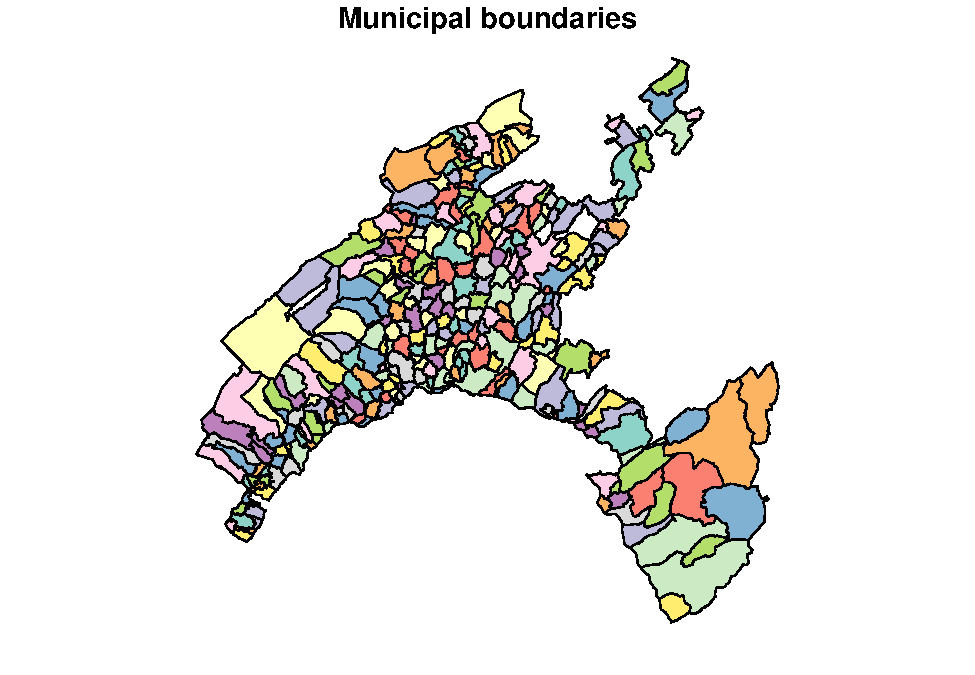
\includegraphics{02-RGIS_files/figure-latex/simple-plot-2} \end{center}

A legend with a continuous color scale is produced by default if the object to be plotted is numeric.

\begin{Shaded}
\begin{Highlighting}[]
\CommentTok{\# Plot based on the value "area" }
\FunctionTok{plot}\NormalTok{(vaud[}\StringTok{"Shape\_Area"}\NormalTok{], }\AttributeTok{reset =} \ConstantTok{FALSE}\NormalTok{)}
\end{Highlighting}
\end{Shaded}

\begin{center}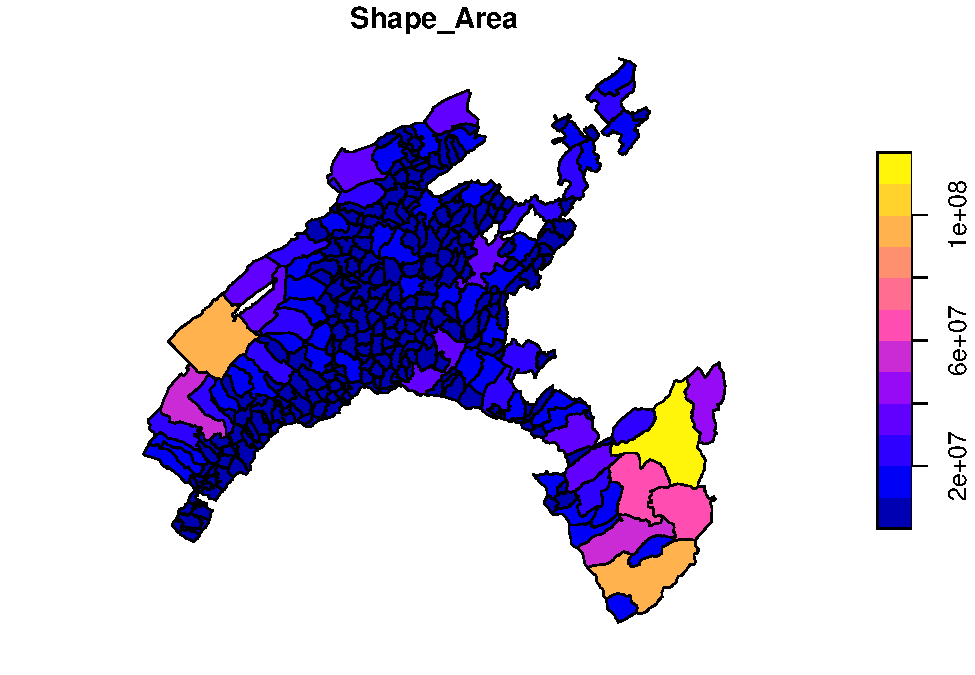
\includegraphics{02-RGIS_files/figure-latex/plot-area-1} \end{center}

Different operations can be performed to customize the map. For instance, you can highlight the municipality of Lausanne in red to show its geographic correspondence, keeping all the other municipalities grey.

\begin{Shaded}
\begin{Highlighting}[]
\CommentTok{\# Extract the boundary of Lausanne}
\NormalTok{Lausanne }\OtherTok{=} \FunctionTok{st\_union}\NormalTok{(vaud[vaud}\SpecialCharTok{$}\NormalTok{Munics }\SpecialCharTok{==} \StringTok{"Lausanne"}\NormalTok{, ])}

\CommentTok{\# Plot the Lausanne municipal boundaries over the map of Canton of Vaud}
\FunctionTok{plot}\NormalTok{(vaud[}\StringTok{"Munics"}\NormalTok{],}\AttributeTok{col=}\StringTok{"grey"}\NormalTok{, }\AttributeTok{reset =} \ConstantTok{FALSE}\NormalTok{, }\AttributeTok{main=}\StringTok{"Canton Vaud, Lausanne"}\NormalTok{)}
\FunctionTok{plot}\NormalTok{(Lausanne, }\AttributeTok{add =} \ConstantTok{TRUE}\NormalTok{, }\AttributeTok{col =} \StringTok{"red"}\NormalTok{)}
\end{Highlighting}
\end{Shaded}

\begin{center}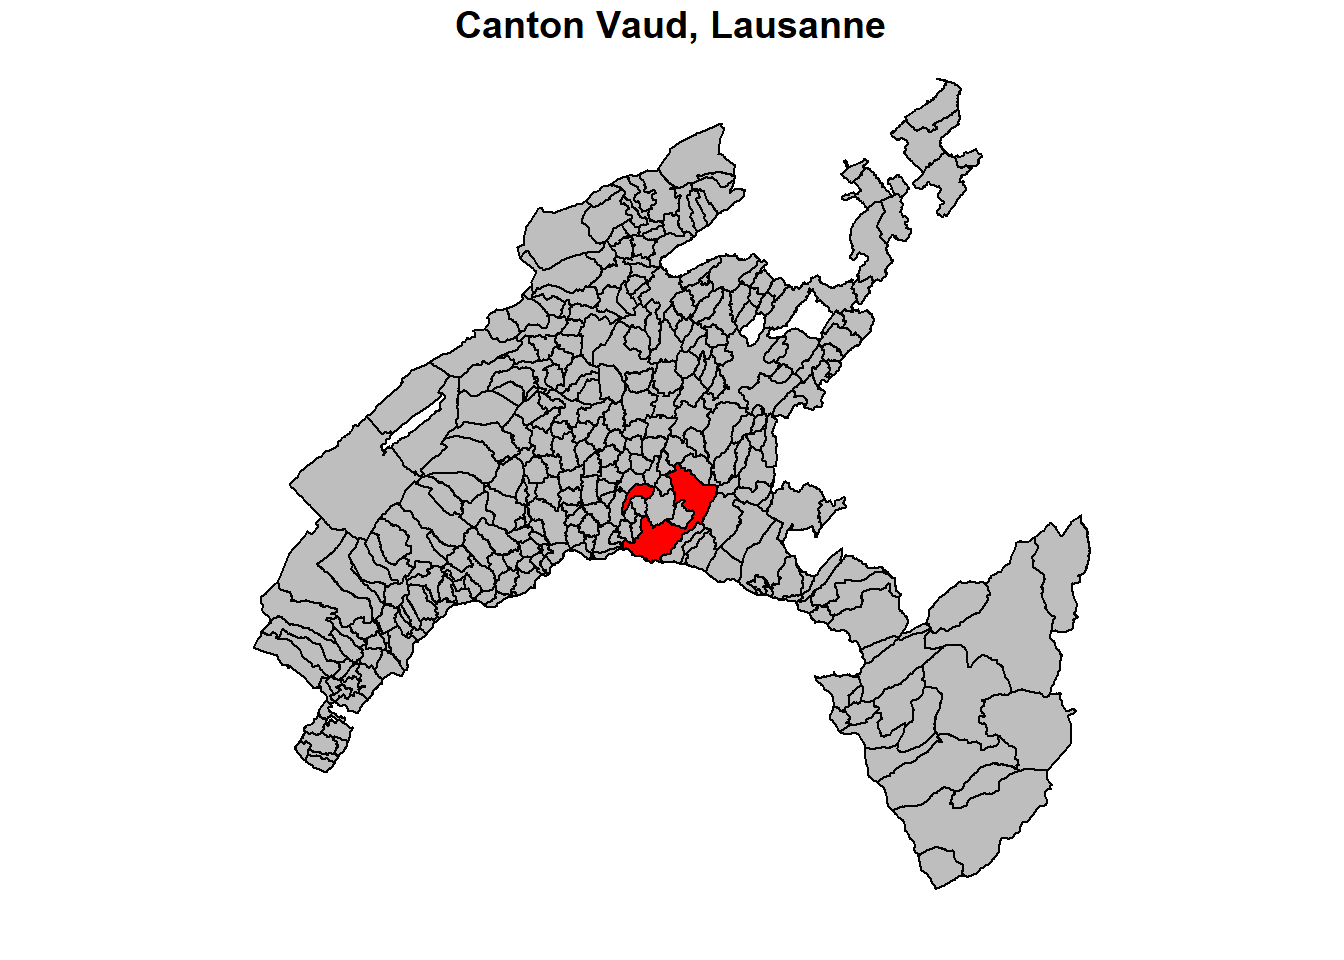
\includegraphics{02-RGIS_files/figure-latex/plot-Lausanne-1} \end{center}

\subsection{Plotting raster dataset}\label{plotting-raster-dataset}

Raster data are different from vector data in that they are referenced to a regular grid of regular (usually square) cells, called pixels. The spatial characteristics of a raster dataset are defined by its spatial resolution (the height and width of each cell) and its origin (typically the upper left corner of the raster grid, which is associated with a location in a coordinate reference system).

Raster data is highly effective for modeling and visualizing continuous spatial phenomena such as elevation, temperature, and precipitation. Each cell in the grid captures a value representing the attribute at that specific location, allowing for smooth and detailed gradients across the study area. This format is also effective in representing categorical variables such as land cover, where each cell is associated with a class value.

Common \textbf{raster formats} used for spatial analyses include:

\begin{enumerate}
\def\labelenumi{\arabic{enumi}.}
\tightlist
\item
  \emph{GeoTIFF (*.tif, *.tiff):}

  \begin{itemize}
  \tightlist
  \item
    A widely used format that includes geographic metadata such as coordinates and projection information, making it easy to integrate with GIS applications.
  \end{itemize}
\item
  \emph{ESRI Grid:}

  \begin{itemize}
  \tightlist
  \item
    A proprietary format developed by ESRI for use with its software, such as ArcGIS. It supports both integer and floating-point grids.
  \end{itemize}
\item
  \emph{Erdas Imagine (*.img):}

  \begin{itemize}
  \tightlist
  \item
    A format developed by ERDAS for its Imagine software, often used for remote sensing data and satellite imagery. It supports large files and multiple bands.
  \end{itemize}
\item
  \emph{NetCDF (*.nc):}

  \begin{itemize}
  \tightlist
  \item
    Stands for Network Common Data Form, used for array-oriented scientific data, including GIS data. It supports multidimensional data arrays, making it suitable for complex environmental and atmospheric data.
  \end{itemize}
\item
  \emph{Hierarchical Data Format (HDF):}

  \begin{itemize}
  \tightlist
  \item
    Similar to NetCDF, HDF is used for managing and storing large amounts of data, especially in scientific computing. It supports various data types and is used for satellite imagery and climate data.
  \end{itemize}
\item
  \emph{ASCII Grid (*.asc):}

  \begin{itemize}
  \tightlist
  \item
    A simple, text-based raster format where each cell value is represented by a number in a grid layout. It's easy to read and edit with a text editor.
  \end{itemize}
\end{enumerate}

These formats vary in terms of compression, metadata support, and suitability for different types of raster data, from simple images to complex scientific datasets.

\subsubsection{Terra package and raster dataset}\label{terra-package-and-raster-dataset}

The package \textbf{terra} provides a variety of specialized classes and functions for importing, processing, analyzing, and visualizing raster datasets \citep{Hijmans_2024}. It is intended to replace the package ``raster'', which has similar data objects and the function syntax as terra package. However, the terra package contains several major improvements, including faster processing speed for large raster.

\subsubsection{Plot raster features}\label{plot-raster-features}

Raster objects can be imported using the function \texttt{rast()} and exported using \texttt{writeRaster()}, specifying the format argument. As a toy example, we will work with the raster *.tif representing the digital elevation model (DEM) of Canton Vaud. Similar to the sf package for plotting vector data, terra also provides \texttt{plot()} methods for its own classes.

\begin{Shaded}
\begin{Highlighting}[]
\CommentTok{\# Load the library terra }
\FunctionTok{library}\NormalTok{(terra)}

\CommentTok{\# Load the raster dataset}
\NormalTok{DEM\_VD }\OtherTok{\textless{}{-}} \FunctionTok{rast}\NormalTok{(}\StringTok{"data/RGIS/DEM100.tif"}\NormalTok{)}

\CommentTok{\# Inspect the raster}
\NormalTok{DEM\_VD}
\end{Highlighting}
\end{Shaded}

\begin{verbatim}
## class       : SpatRaster 
## dimensions  : 881, 912, 1  (nrow, ncol, nlyr)
## resolution  : 100, 100  (x, y)
## extent      : 494300, 585500, 115150, 203250  (xmin, xmax, ymin, ymax)
## coord. ref. : CH1903 / LV03 (EPSG:21781) 
## source      : DEM100.tif 
## name        : DEM100 
## min value   :  372.0 
## max value   : 3193.2
\end{verbatim}

\begin{Shaded}
\begin{Highlighting}[]
\CommentTok{\# Plot raster dataset}
\FunctionTok{plot}\NormalTok{(DEM\_VD, }\AttributeTok{main=}\StringTok{"DEM"}\NormalTok{)}
\end{Highlighting}
\end{Shaded}

\begin{center}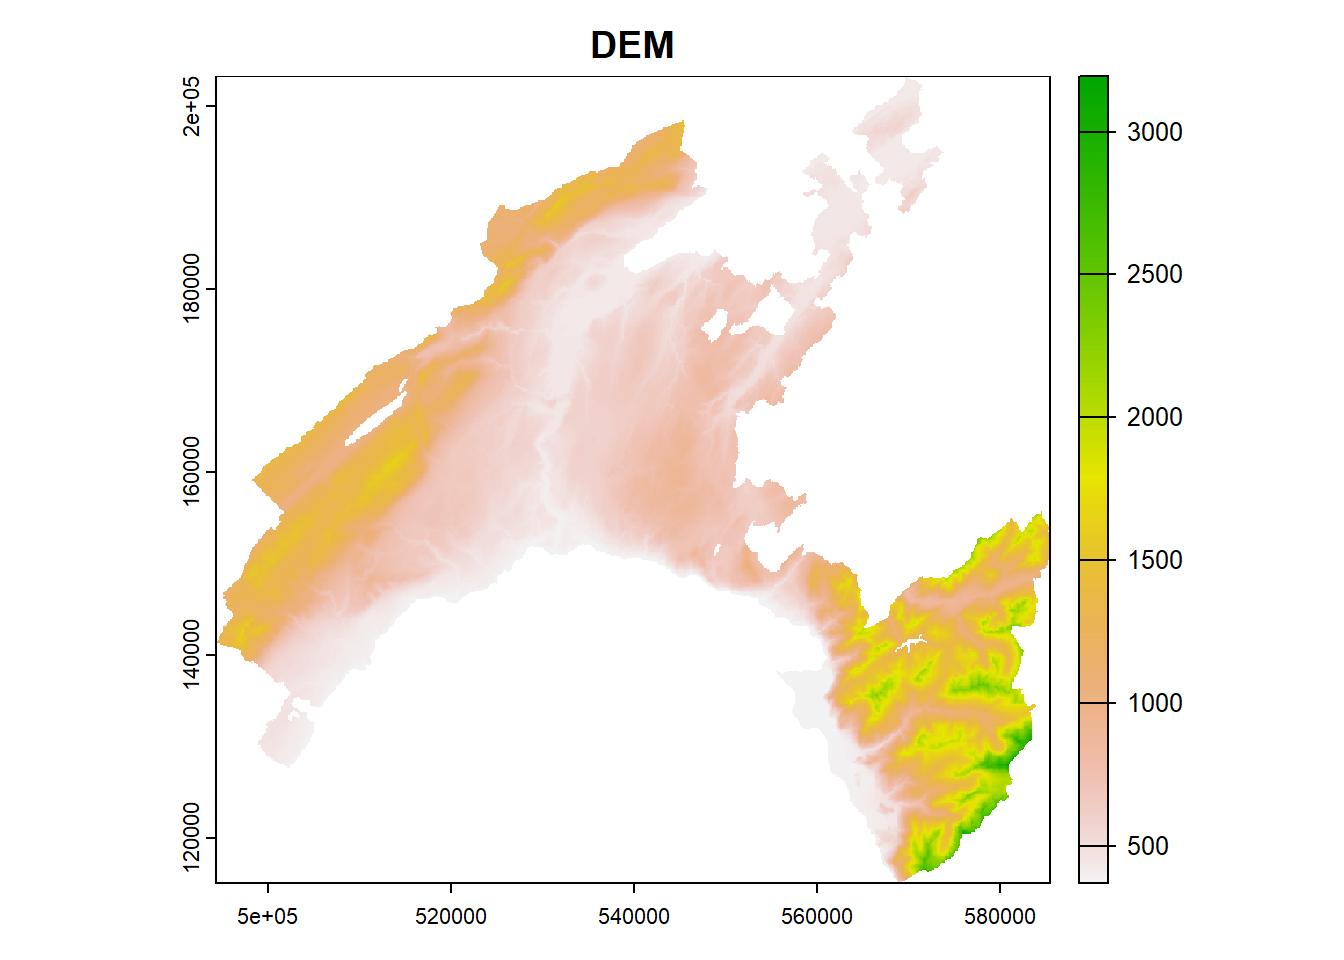
\includegraphics{02-RGIS_files/figure-latex/plot-raster-1} \end{center}

\subsection{Geodata manipulation}\label{geodata-manipulation}

In this section, we explore some basic manipulations with vector and raster geodata. This will be useful in the following chapters of this book.

\subsubsection{Manipulate tabular datasets}\label{manipulate-tabular-datasets}

In a vector dataset, the characteristics associated with geospatial features are stored in the attribute table. Each feature in the vector dataset is linked to a row in the table, with its characteristics organized into columns. Columns, also known as fields, store the various attributes associated with the features.

Thematic attributes stored in separate tabular dataset (such as census data, environmental monitoring stations, public health, or traffic data) can be imported and added to the attribute table of a given vector datased if the two dataset are referred to the same spatial features.

While tabular dataset can be delivered in different format (such as *.dbf, *.xlsx, *.txt), the most widely used format is *\textbf{.csv} (comma-separated values). As for other tabular format, *.csv is structured into rows and columns, where each column is separated by a comma. The first row often contains the column headers (field names), which describes the attribute in each column. The main advantages of this format compared with other formats are:

\begin{itemize}
\tightlist
\item
  \emph{Simplicity}: easy to create, read, and edit.
\item
  \emph{Lightweight}: files are typically small and easy to transfer.
\item
  \emph{Compatibility}: supported by most data processing tools and software.
\end{itemize}

In most cases, data need to be reworked before beeing visualized and analyzed in R. Common tasks include: selecting subsets of rows or columns from the attribute table, rename a field, calculate new variables from the raw data values, compute summary statistics, combine data from different sources. To this end, the package \textbf{dplyr} \citep{Wickham_et_al_2003} provides consistent set of functions that help you to solve the most common data manipulation challenges. We explore some of them in the following code chunks.

As a toy example, we will work with the the Swioss population census dataset 2020.

\begin{Shaded}
\begin{Highlighting}[]
\CommentTok{\# Load ths library dply}
\FunctionTok{library}\NormalTok{(dplyr)}

\CommentTok{\# Load tabular dataset}
\NormalTok{Swisscensus\_2020 }\OtherTok{\textless{}{-}} \FunctionTok{read.csv}\NormalTok{(}\StringTok{"data/RGIS/census2020.csv"}\NormalTok{)}

\CommentTok{\# Inspect the element }
\FunctionTok{str}\NormalTok{(Swisscensus\_2020)}
\end{Highlighting}
\end{Shaded}

\begin{verbatim}
## 'data.frame':    2145 obs. of  35 variables:
##  $ ID_0                 : int  1 2 3 4 5 6 7 8 9 10 ...
##  $ ID                   : int  1 2 3 4 5 6 7 8 9 10 ...
##  $ p_infrastructure     : num  0.131 0.302 0.178 0.133 0.199 ...
##  $ p_forested           : num  0.307 0.28 0.287 0.291 0.332 ...
##  $ p_agriculture        : num  0.502 0.401 0.526 0.554 0.464 ...
##  $ p_improductible      : num  0.05815 0.01133 0.01077 0.025 0.00766 ...
##  $ surface_polygone     : num  791 1059 743 1360 653 ...
##  $ natural_growth_1000  : num  -1.001 2.115 4.65 2.119 0.528 ...
##  $ density              : num  255 1160 755 279 581 ...
##  $ dependency_ratio     : num  60.1 63.4 68.6 67.4 62.9 ...
##  $ migration_intern     : num  11.014 -6.1 -0.537 9.534 -2.905 ...
##  $ migration            : num  3.5 5.61 1.07 1.32 5.02 ...
##  $ p_employment         : num  0.105 0.415 0.109 0.14 0.364 ...
##  $ primary_sector       : num  0.19388 0.06495 0 2.12 0.00187 ...
##  $ secondary_sector     : num  0.148 1.724 0 2.8 0.045 ...
##  $ tertiary_sector      : num  1.9898 7.6414 0.3155 16.1 0.0569 ...
##  $ p_social_assistance  : num  1.31 3.19 1.13 1.25 1.27 ...
##  $ p_new_buildings      : num  1.514 0.732 0.179 0.8 0.529 ...
##  $ p_new_housings       : num  5.048 4.552 0.179 1.333 1.059 ...
##  $ p_cinema             : num  0 0.0195 0 0 0 ...
##  $ p_museum             : num  0.000993 0 0 0 0.000264 ...
##  $ p_culture_institution: num  0.01142 0.00667 0.00588 0.00816 0.00606 ...
##  $ size_households      : num  2.28 2.19 2.37 2.39 2.38 ...
##  $ p_new_entreprise     : num  0.00497 0.00407 0.00267 0.00421 0.00369 ...
##  $ p_weddings           : num  2.5 4.8 4.65 2.65 1.85 ...
##  $ p_foreigners         : num  14.4 29 17.3 15.8 17.4 ...
##  $ p_individual_houses  : num  69.2 54.7 71.6 69.1 74.7 ...
##  $ Population           : num  2014 12289 5610 3801 3795 ...
##  $ p_pop_19             : num  19.8 22.3 21.9 22.1 19.3 ...
##  $ p_pop_65             : num  18.5 18.6 14.1 21.5 20.4 ...
##  $ lat                  : num  0.571 0.562 0.566 0.582 0.562 ...
##  $ long                 : num  0.735 0.738 0.756 0.719 0.748 ...
##  $ zab_2022             : num  69.6 285.9 92.4 126.6 102.8 ...
##  $ net_income_h         : num  57603 36521 45237 45791 48875 ...
##  $ p_transport          : num  5.06 7.69 5.11 4.55 4.89 ...
\end{verbatim}

\begin{Shaded}
\begin{Highlighting}[]
\CommentTok{\# Create a subset including only Land Use information}
\NormalTok{Swisscensus2020\_LU }\OtherTok{=} \FunctionTok{subset}\NormalTok{(Swisscensus\_2020, }\AttributeTok{select =} \FunctionTok{c}\NormalTok{(}\DecValTok{2}\SpecialCharTok{:}\DecValTok{6}\NormalTok{))}

\FunctionTok{str}\NormalTok{(Swisscensus2020\_LU)}
\end{Highlighting}
\end{Shaded}

\begin{verbatim}
## 'data.frame':    2145 obs. of  5 variables:
##  $ ID              : int  1 2 3 4 5 6 7 8 9 10 ...
##  $ p_infrastructure: num  0.131 0.302 0.178 0.133 0.199 ...
##  $ p_forested      : num  0.307 0.28 0.287 0.291 0.332 ...
##  $ p_agriculture   : num  0.502 0.401 0.526 0.554 0.464 ...
##  $ p_improductible : num  0.05815 0.01133 0.01077 0.025 0.00766 ...
\end{verbatim}

\begin{Shaded}
\begin{Highlighting}[]
\CommentTok{\# Rename a column for better understanding}
\NormalTok{CH2020\_LU }\OtherTok{\textless{}{-}} \FunctionTok{rename}\NormalTok{(Swisscensus2020\_LU, }\AttributeTok{Urban=}\NormalTok{p\_infrastructure)}
\FunctionTok{head}\NormalTok{(CH2020\_LU)}
\end{Highlighting}
\end{Shaded}

\begin{verbatim}
##   ID      Urban p_forested p_agriculture p_improductible
## 1  1 0.13147914  0.3072061     0.5018963     0.058154235
## 2  2 0.30217186  0.2804533     0.4013220     0.011331445
## 3  3 0.17765814  0.2866756     0.5262450     0.010767160
## 4  4 0.13308823  0.2911765     0.5536765     0.025000000
## 5  5 0.19908116  0.3323124     0.4640123     0.007656968
## 6  6 0.08712121  0.2058081     0.6830808     0.011363636
\end{verbatim}

\subsubsection{Pipes: chaining of multiple operations}\label{pipes-chaining-of-multiple-operations}

Pipes allow for the chaining of multiple operations in a unique sequence, which makes the code easier to understand and reduces the need for nested function calls.

The use of pipes in R, primarily facilitated by the \textbf{magrittr} package and now natively supported in base R (R version 4.1.0 and above), is a powerful way to write clear and readable code. The function pipe is represented by the symbol \texttt{\%\textgreater{}\%}. When a pipe is placed on the right side of an object or function, the output from the function is passed as the first argument to the next function after the pipe.

Below is a simple example of using the pipe operator with the function \texttt{select()}, used to select the the fields related to the land use in the Swiss census dataset corresponding to a population density less than 100.

\begin{Shaded}
\begin{Highlighting}[]
\NormalTok{LU\_dens100 }\OtherTok{\textless{}{-}} 
\NormalTok{  Swisscensus\_2020 }\SpecialCharTok{\%\textgreater{}\%}
  \FunctionTok{filter}\NormalTok{(density }\SpecialCharTok{\textless{}} \DecValTok{100}\NormalTok{) }\SpecialCharTok{\%\textgreater{}\%}
  \FunctionTok{select}\NormalTok{(}\DecValTok{2}\SpecialCharTok{:}\DecValTok{6}\NormalTok{)}

\FunctionTok{str}\NormalTok{(LU\_dens100)}
\end{Highlighting}
\end{Shaded}

\begin{verbatim}
## 'data.frame':    660 obs. of  5 variables:
##  $ ID              : int  23 81 114 182 211 226 309 322 325 326 ...
##  $ p_infrastructure: num  0.0514 0.0635 0.0483 0.0785 0.0727 ...
##  $ p_forested      : num  0.455 0.453 0.614 0.366 0.203 ...
##  $ p_agriculture   : num  0.479 0.487 0.32 0.521 0.683 ...
##  $ p_improductible : num  0.01712 0.00219 0.01521 0.03217 0.04156 ...
\end{verbatim}

\subsubsection{Join table}\label{join-table}

A tabular dataset can be joined to the attribute table of a vector dataset by specifying the name of the columns in the two tables used for merging. To this end, we can use the function \texttt{merge()} included in the package sp .

\begin{Shaded}
\begin{Highlighting}[]
\NormalTok{Vaud\_census\_2020 }\OtherTok{\textless{}{-}} \FunctionTok{merge}\NormalTok{(}\AttributeTok{x=}\NormalTok{vaud, }\AttributeTok{y=}\NormalTok{Swisscensus\_2020,}
                             \AttributeTok{by.x=}\StringTok{"Code"}\NormalTok{, }
                             \AttributeTok{by.y=}\StringTok{"ID"}\NormalTok{,}
                             \AttributeTok{all.x=}\ConstantTok{TRUE}\NormalTok{)}

\CommentTok{\# Plot based on a joined attribute}
\FunctionTok{plot}\NormalTok{(Vaud\_census\_2020[}\StringTok{"p\_agriculture"}\NormalTok{])}
\end{Highlighting}
\end{Shaded}

\begin{center}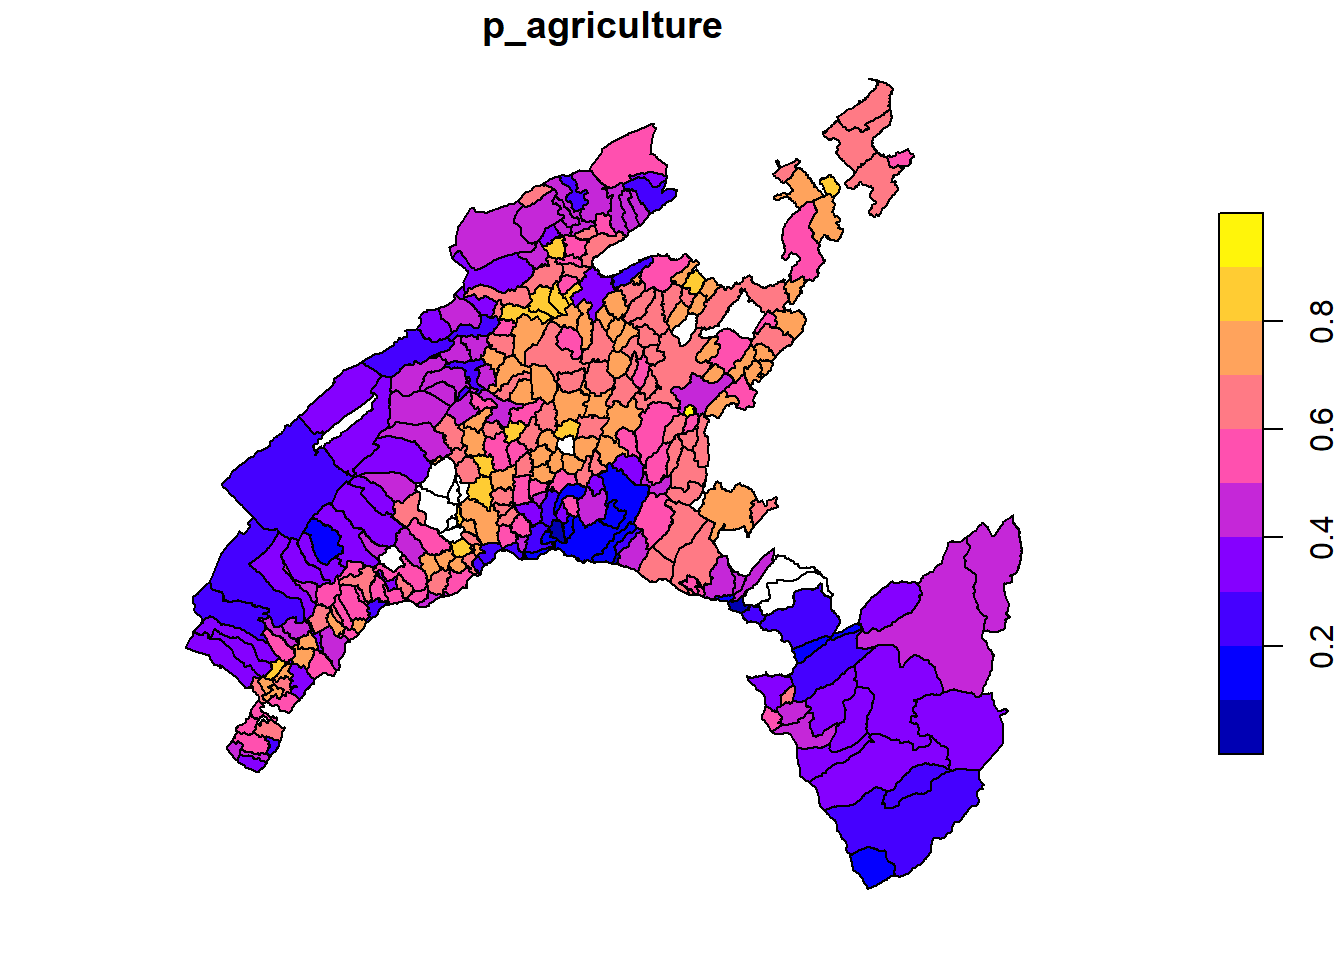
\includegraphics{02-RGIS_files/figure-latex/merge-tab-1} \end{center}

\subsubsection{Mapping with ggplot2}\label{mapping-with-ggplot2}

Mapping in R can be efficiently achieved using the powerful visualization package \textbf{ggplot2}, especially when combined with additional packages like sf. These tools togheter enable users to create detailed and customized maps for spatial data analysis and visualization. In particular sf facilitates the handling of complex spatial data structures, making it possible to create intricate and informative maps.

In the following example we crate an aesthetic map of Canton Vaud based on the percentage of agricultural land use by municipality. Aesthetic mappings describe how the attributes of the geodata are mapped to the visual properties (aesthetics) of the plot. The command aesthetics -- \texttt{aes()} -- control the appearance of the plot elements, such as points, lines, bars, and so on.

\begin{Shaded}
\begin{Highlighting}[]
\CommentTok{\# load the library gglpt2}
\FunctionTok{library}\NormalTok{ (ggplot2)}

\CommentTok{\# Install viridis color scale as a package }
\FunctionTok{install.packages}\NormalTok{(}\StringTok{"viridis"}\NormalTok{, }\AttributeTok{repos=}\StringTok{"http://cran.us.r{-}project.org"}\NormalTok{)}
\end{Highlighting}
\end{Shaded}

\begin{verbatim}
## package 'viridis' successfully unpacked and MD5 sums checked
## 
## The downloaded binary packages are in
##  C:\Users\mtonini1\AppData\Local\Temp\RtmpiyDQ83\downloaded_packages
\end{verbatim}

\begin{Shaded}
\begin{Highlighting}[]
\FunctionTok{library}\NormalTok{(viridis)}

\CommentTok{\# Use ggplot2 for mapping}
\FunctionTok{ggplot}\NormalTok{(Vaud\_census\_2020) }\SpecialCharTok{+}
  \FunctionTok{geom\_sf}\NormalTok{(}\FunctionTok{aes}\NormalTok{(}\AttributeTok{fill =}\NormalTok{ p\_agriculture)) }\SpecialCharTok{+}
  \FunctionTok{scale\_fill\_viridis\_c}\NormalTok{(}\AttributeTok{option =} \StringTok{"viridis"}\NormalTok{, }\AttributeTok{name =} \StringTok{"Agri (\%)"}\NormalTok{) }\SpecialCharTok{+}
  \FunctionTok{theme\_minimal}\NormalTok{() }\SpecialCharTok{+}
  \FunctionTok{labs}\NormalTok{(}\AttributeTok{title =} \StringTok{"Agrucultural land use"}\NormalTok{,}
       \AttributeTok{subtitle =} \StringTok{"Canton vaud {-} census 2020"}\NormalTok{)}
\end{Highlighting}
\end{Shaded}

\begin{center}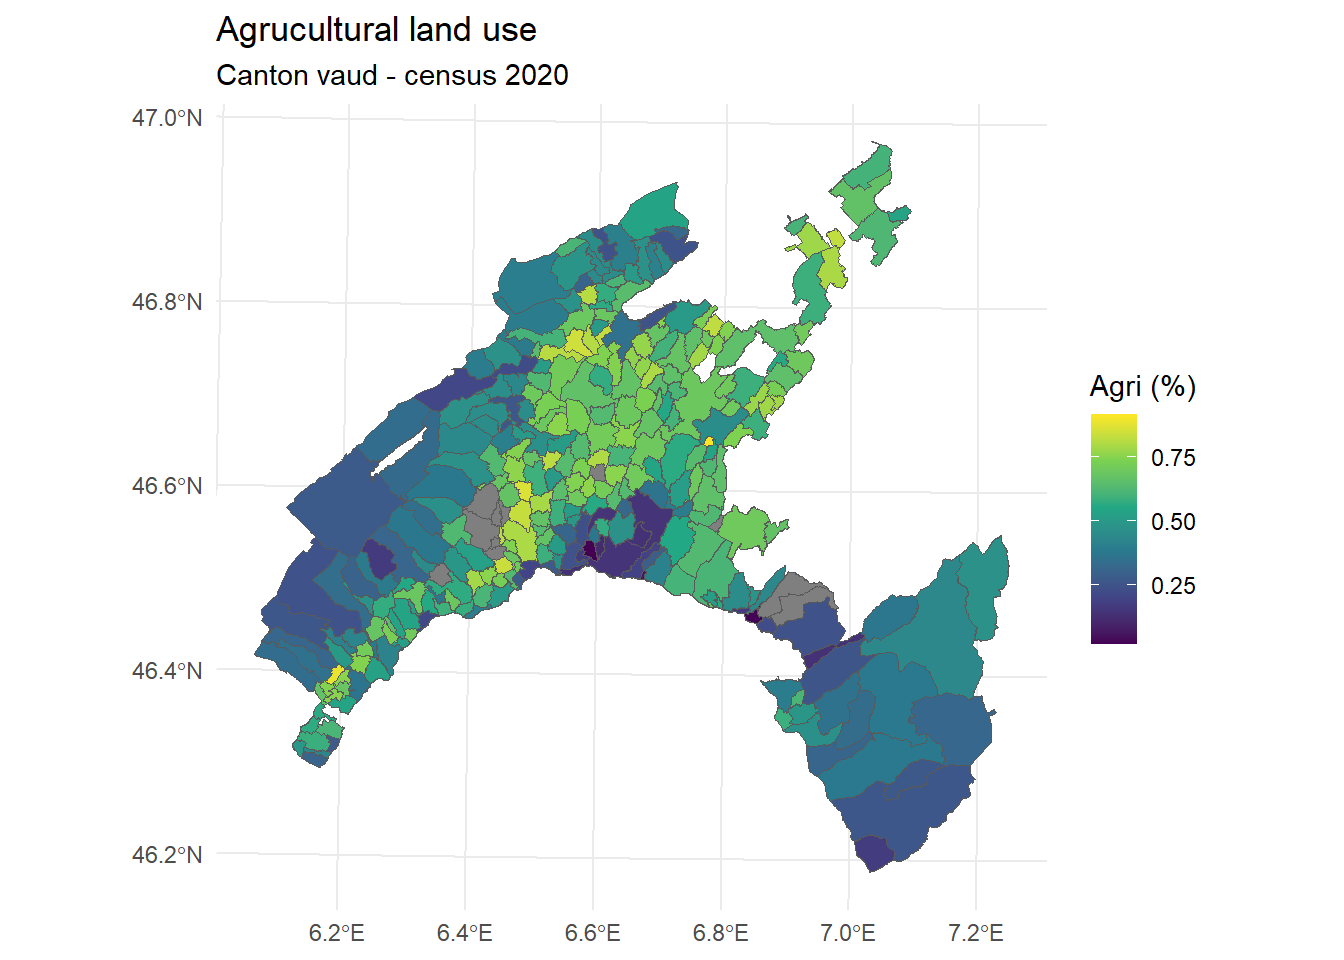
\includegraphics{02-RGIS_files/figure-latex/mapping-1} \end{center}

\subsubsection{Cropping ratser}\label{cropping-ratser}

Many projects in geosciences require integrating raster data covering an exension larger than the study area. In these scenarios, raster cropping and masking are essential for standardizing the spatial extent of the input data. These operations help to minimize memory usage and computational resources needed for subsequent analysis, and often represnet a crucial pre-processing step before generating detailed and visually appealing maps incorporating raster data.

The first check you need to perform when importing data from different sources is to verify whether the \textbf{coordinate reference systems (CRS)} of the input geodatasets are consistent. To this end, simply type the names of the geodatasets and check the ``coord. ref.'' attribute. For a detailed description of the coordinate reference system, use the \texttt{crs()} function. If necessary, re-project one of the spatial layers using the \texttt{project()} function, specifying the CRS of the other dataset to ensure their extents perfectly overlap.

\begin{Shaded}
\begin{Highlighting}[]
\CommentTok{\# Verify CRS}
\NormalTok{DEM\_VD}
\end{Highlighting}
\end{Shaded}

\begin{verbatim}
## class       : SpatRaster 
## dimensions  : 881, 912, 1  (nrow, ncol, nlyr)
## resolution  : 100, 100  (x, y)
## extent      : 494300, 585500, 115150, 203250  (xmin, xmax, ymin, ymax)
## coord. ref. : CH1903 / LV03 (EPSG:21781) 
## source      : DEM100.tif 
## name        : DEM100 
## min value   :  372.0 
## max value   : 3193.2
\end{verbatim}

\begin{Shaded}
\begin{Highlighting}[]
\NormalTok{vaud}
\end{Highlighting}
\end{Shaded}

\begin{verbatim}
## Simple feature collection with 315 features and 4 fields
## Geometry type: POLYGON
## Dimension:     XY
## Bounding box:  xmin: 2494306 ymin: 1115149 xmax: 2585462 ymax: 1203493
## Projected CRS: CH1903+ / LV95
## First 10 features:
##    Shape_Leng Shape_Area         Munics Code                       geometry
## 1    30546.68   24178457        Payerne 5822 POLYGON ((2559434 1183900, ...
## 2    21404.88   23354685     Rossinière 5842 POLYGON ((2568027 1143632, ...
## 3    27146.69   23190781       Vallorbe 5764 POLYGON ((2519472 1176171, ...
## 4    31110.58   22858943        Puidoux 5607 POLYGON ((2551941 1152936, ...
## 5    28268.14   22501915        Baulmes 5745 POLYGON ((2524665 1180813, ...
## 6    26122.21   22002176     Corbeyrier 5404 POLYGON ((2565278 1132847, ...
## 7    33182.64   20915807 Vully-les-Lacs 5464 POLYGON ((2565363 1195281, ...
## 8    29224.24   20772714        Bassins 5703 POLYGON ((2508540 1146203, ...
## 9    20254.18   19791177  Mont-la-Ville 5491 POLYGON ((2519784 1169416, ...
## 10   30004.81   19487486       Avenches 5451 POLYGON ((2570746 1194939, ...
\end{verbatim}

\begin{Shaded}
\begin{Highlighting}[]
\CommentTok{\# Project the DEM data using the CRS of the shapefile }
\NormalTok{demVD\_prj }\OtherTok{=} \FunctionTok{project}\NormalTok{(DEM\_VD, }\FunctionTok{crs}\NormalTok{(vaud))}

\CommentTok{\# Verify again}
\FunctionTok{plot}\NormalTok{(DEM\_VD)}
\end{Highlighting}
\end{Shaded}

\begin{center}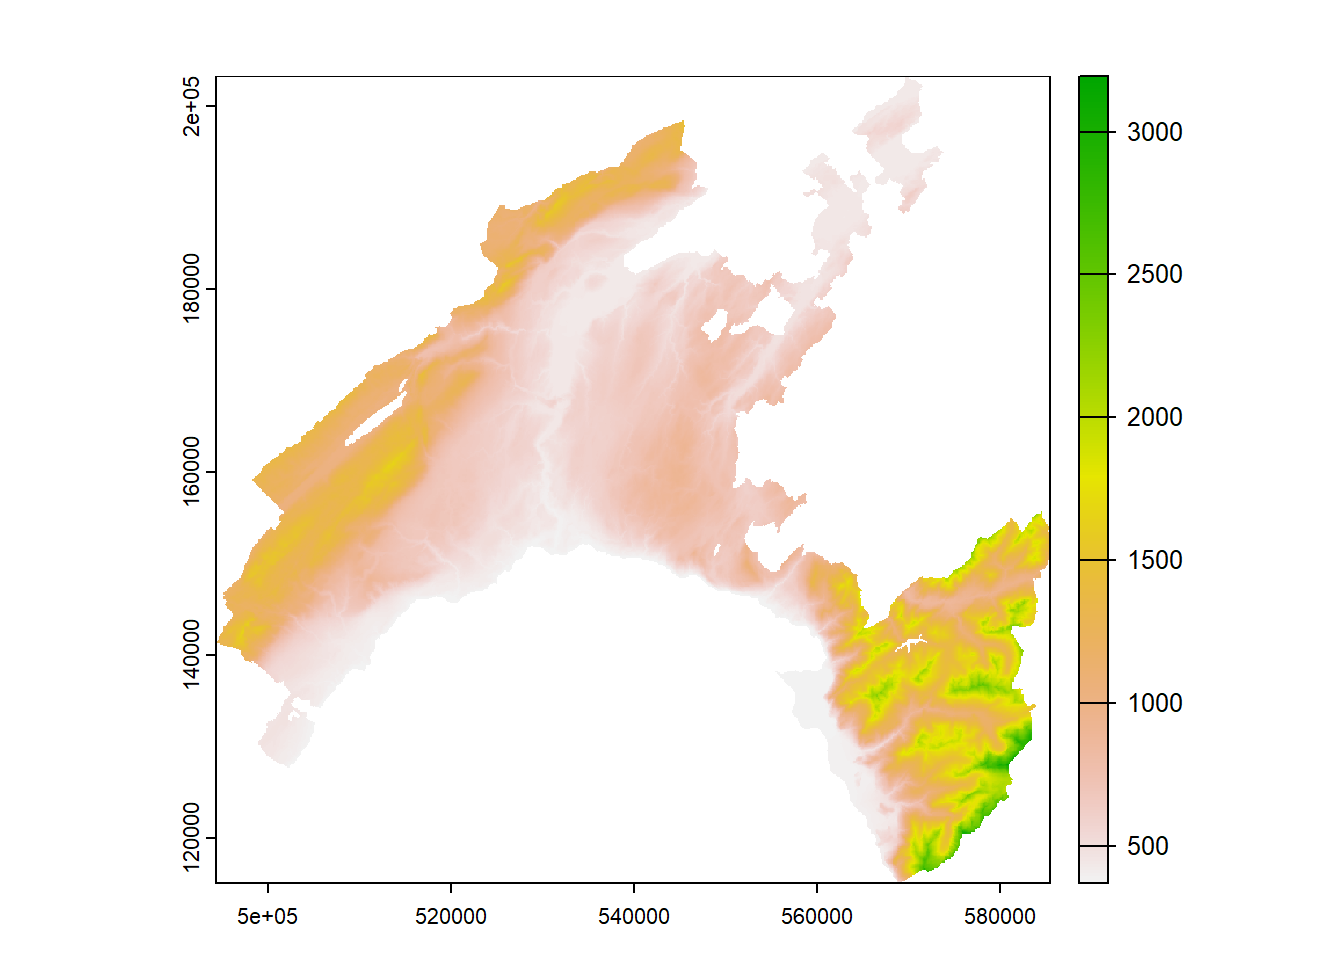
\includegraphics{02-RGIS_files/figure-latex/project-1} \end{center}

\begin{Shaded}
\begin{Highlighting}[]
\FunctionTok{plot}\NormalTok{(demVD\_prj)}
\end{Highlighting}
\end{Shaded}

\begin{center}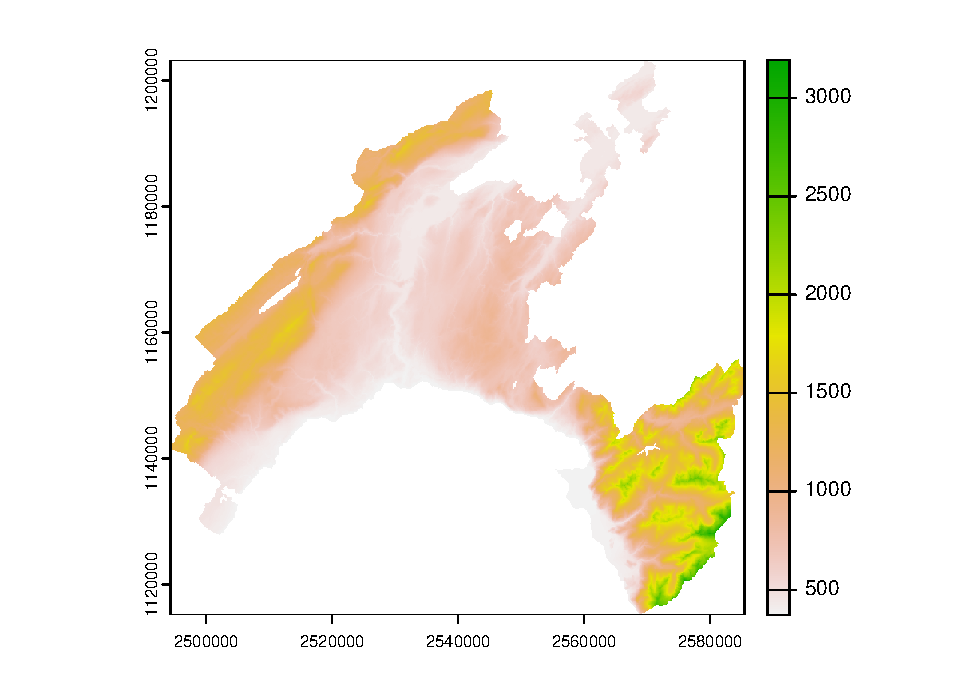
\includegraphics{02-RGIS_files/figure-latex/project-2} \end{center}

\begin{Shaded}
\begin{Highlighting}[]
\CommentTok{\# Extract the municipality of Lausanne}
\NormalTok{Lausanne }\OtherTok{\textless{}{-}} \FunctionTok{filter}\NormalTok{(vaud, Munics }\SpecialCharTok{==} \StringTok{"Lausanne"}\NormalTok{)}

\CommentTok{\# Crop the DEM to the extent of Lausanne (bounding box)}
\NormalTok{DEM\_Lausanne\_cropped }\OtherTok{\textless{}{-}} \FunctionTok{crop}\NormalTok{(demVD\_prj, Lausanne)}

\CommentTok{\# Mask the cropped DEM using the Lausanne polygon to get the exact shape}
\NormalTok{DEM\_Lausanne }\OtherTok{\textless{}{-}} \FunctionTok{mask}\NormalTok{(DEM\_Lausanne\_cropped, Lausanne)}

\CommentTok{\# Plot the DEM}
\FunctionTok{plot}\NormalTok{(DEM\_Lausanne, }\AttributeTok{main =} \StringTok{"DEM of Lausanne"}\NormalTok{)}

\CommentTok{\# Add the Lausanne polygon outline}
\FunctionTok{plot}\NormalTok{(}\FunctionTok{st\_geometry}\NormalTok{(Lausanne), }\AttributeTok{add =} \ConstantTok{TRUE}\NormalTok{, }\AttributeTok{border =} \StringTok{"red"}\NormalTok{, }\AttributeTok{lwd =} \DecValTok{2}\NormalTok{)}
\end{Highlighting}
\end{Shaded}

\begin{center}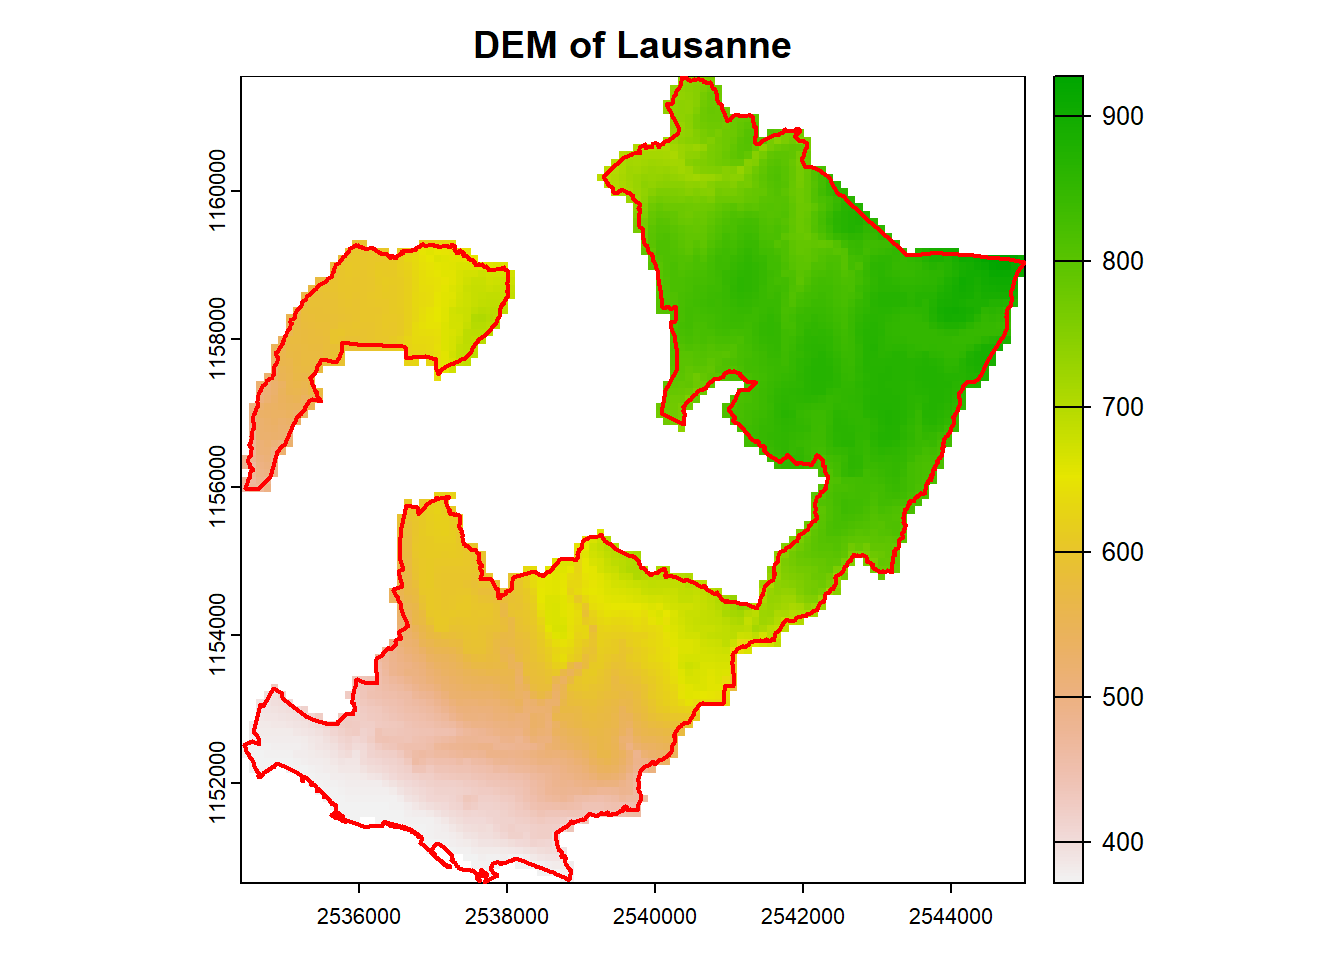
\includegraphics{02-RGIS_files/figure-latex/cropping-1} \end{center}

\subsubsection{Display the categorical variables of a raster}\label{display-the-categorical-variables-of-a-raster}

Categorical variables, also known as qualitative variables, are variables that represent distinct groups or categories. These variables are typically non-numeric and can be divided into a finite number of categories or levels. Categorical variables are often used to represent characteristics or attributes that do not have a natural ordering.

Land use classes of a raster dataset are a common example of categorical variables. Each class represents a distinct type of land use labeled with names or, mostly, numeric codes.

To understand the characteristics of the categorical variables, you can plot the ``Land Cover'' raster dataset by using its original classes. To visualize the data you need to perform few data manipulations before.

\begin{Shaded}
\begin{Highlighting}[]
\CommentTok{\# Load the raster data}
\NormalTok{landCover }\OtherTok{\textless{}{-}} \FunctionTok{rast}\NormalTok{(}\StringTok{"data/RGIS/landCover.tif"}\NormalTok{)}

\CommentTok{\# Inspect the raster}
\NormalTok{landCover}
\end{Highlighting}
\end{Shaded}

\begin{verbatim}
## class       : SpatRaster 
## dimensions  : 3524, 3647, 1  (nrow, ncol, nlyr)
## resolution  : 25, 25  (x, y)
## extent      : 494300, 585475, 115150, 203250  (xmin, xmax, ymin, ymax)
## coord. ref. : CH1903 / LV03 (EPSG:21781) 
## source      : landCover.tif 
## name        : landCover 
## min value   :        11 
## max value   :        62
\end{verbatim}

\begin{Shaded}
\begin{Highlighting}[]
\CommentTok{\# Plot the raster (using codes)}
\FunctionTok{plot}\NormalTok{ (landCover)}
\end{Highlighting}
\end{Shaded}

\begin{center}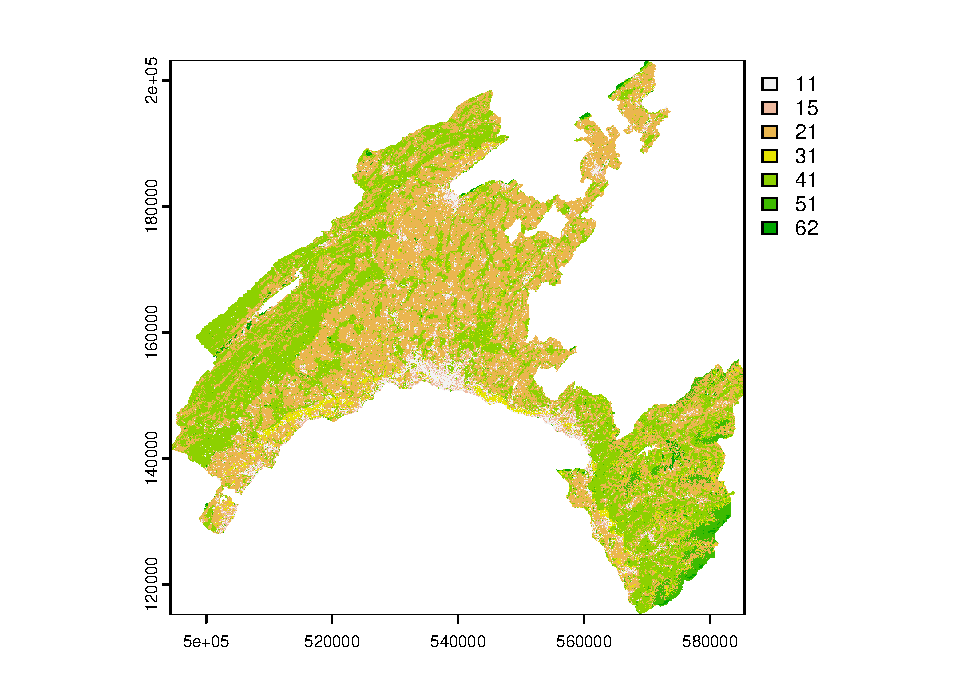
\includegraphics{02-RGIS_files/figure-latex/landCover-map-1} \end{center}

\begin{Shaded}
\begin{Highlighting}[]
\CommentTok{\# Convert the raster as a factor to represent categorical data}
\NormalTok{landCover }\OtherTok{\textless{}{-}} \FunctionTok{as.factor}\NormalTok{(}\FunctionTok{rast}\NormalTok{(}\StringTok{"data/RGIS/landCover.tif"}\NormalTok{))}

\CommentTok{\# Inspect the current levels (classes) of the raster}
\NormalTok{current\_levels }\OtherTok{\textless{}{-}} \FunctionTok{levels}\NormalTok{(landCover)[[}\DecValTok{1}\NormalTok{]]}
\FunctionTok{print}\NormalTok{(current\_levels)}
\end{Highlighting}
\end{Shaded}

\begin{verbatim}
##   ID landCover
## 1 11        11
## 2 15        15
## 3 21        21
## 4 31        31
## 5 41        41
## 6 51        51
## 7 62        62
\end{verbatim}

\begin{Shaded}
\begin{Highlighting}[]
\CommentTok{\# Define a vector of new class names (descriptions)}
\NormalTok{new\_class\_names }\OtherTok{\textless{}{-}} \FunctionTok{c}\NormalTok{(}
 \StringTok{"11"} \OtherTok{=} \StringTok{"Impermeable man{-}made"}\NormalTok{,}
 \StringTok{"15"} \OtherTok{=} \StringTok{"Permeable man{-}made"}\NormalTok{,}
 \StringTok{"21"} \OtherTok{=} \StringTok{"Herbaceous vegetation"}\NormalTok{,}
 \StringTok{"31"} \OtherTok{=} \StringTok{"Shrub vegetation"}\NormalTok{,}
 \StringTok{"41"} \OtherTok{=} \StringTok{"Forest"}\NormalTok{,}
 \StringTok{"51"} \OtherTok{=} \StringTok{"No vegetation"}\NormalTok{,}
 \StringTok{"62"} \OtherTok{=} \StringTok{"Glacier and water body"}\NormalTok{)}

\CommentTok{\# Ensure that new class names match the existing levels}
\NormalTok{current\_levels}\SpecialCharTok{$}\NormalTok{landCover }\OtherTok{\textless{}{-}}\NormalTok{ new\_class\_names[}\FunctionTok{as.character}\NormalTok{(current\_levels}\SpecialCharTok{$}\NormalTok{ID)]}

\CommentTok{\# Apply the new class names to the levels of the raster}
\FunctionTok{levels}\NormalTok{(landCover) }\OtherTok{\textless{}{-}}\NormalTok{ current\_levels}

\CommentTok{\# Verify the new levels}
\FunctionTok{print}\NormalTok{(}\FunctionTok{levels}\NormalTok{(landCover))}
\end{Highlighting}
\end{Shaded}

\begin{verbatim}
## [[1]]
##   ID              landCover
## 1 11   Impermeable man-made
## 2 15     Permeable man-made
## 3 21  Herbaceous vegetation
## 4 31       Shrub vegetation
## 5 41                 Forest
## 6 51          No vegetation
## 7 62 Glacier and water body
\end{verbatim}

\begin{Shaded}
\begin{Highlighting}[]
\CommentTok{\# Create a color palette with enough colors for all classes}

\FunctionTok{library}\NormalTok{(RColorBrewer)}

\NormalTok{num\_classes }\OtherTok{\textless{}{-}} \FunctionTok{length}\NormalTok{(new\_class\_names)}
\NormalTok{color\_palette }\OtherTok{\textless{}{-}} \FunctionTok{colorRampPalette}\NormalTok{(}\FunctionTok{brewer.pal}\NormalTok{(}\DecValTok{8}\NormalTok{, }\StringTok{"Set3"}\NormalTok{))(num\_classes)}

\CommentTok{\# Plot the land cover data with the custom color palette}
\FunctionTok{plot}\NormalTok{(landCover, }\AttributeTok{col =}\NormalTok{ color\_palette, }\AttributeTok{main =} \StringTok{"Land Cover Classes"}\NormalTok{)}
\end{Highlighting}
\end{Shaded}

\begin{center}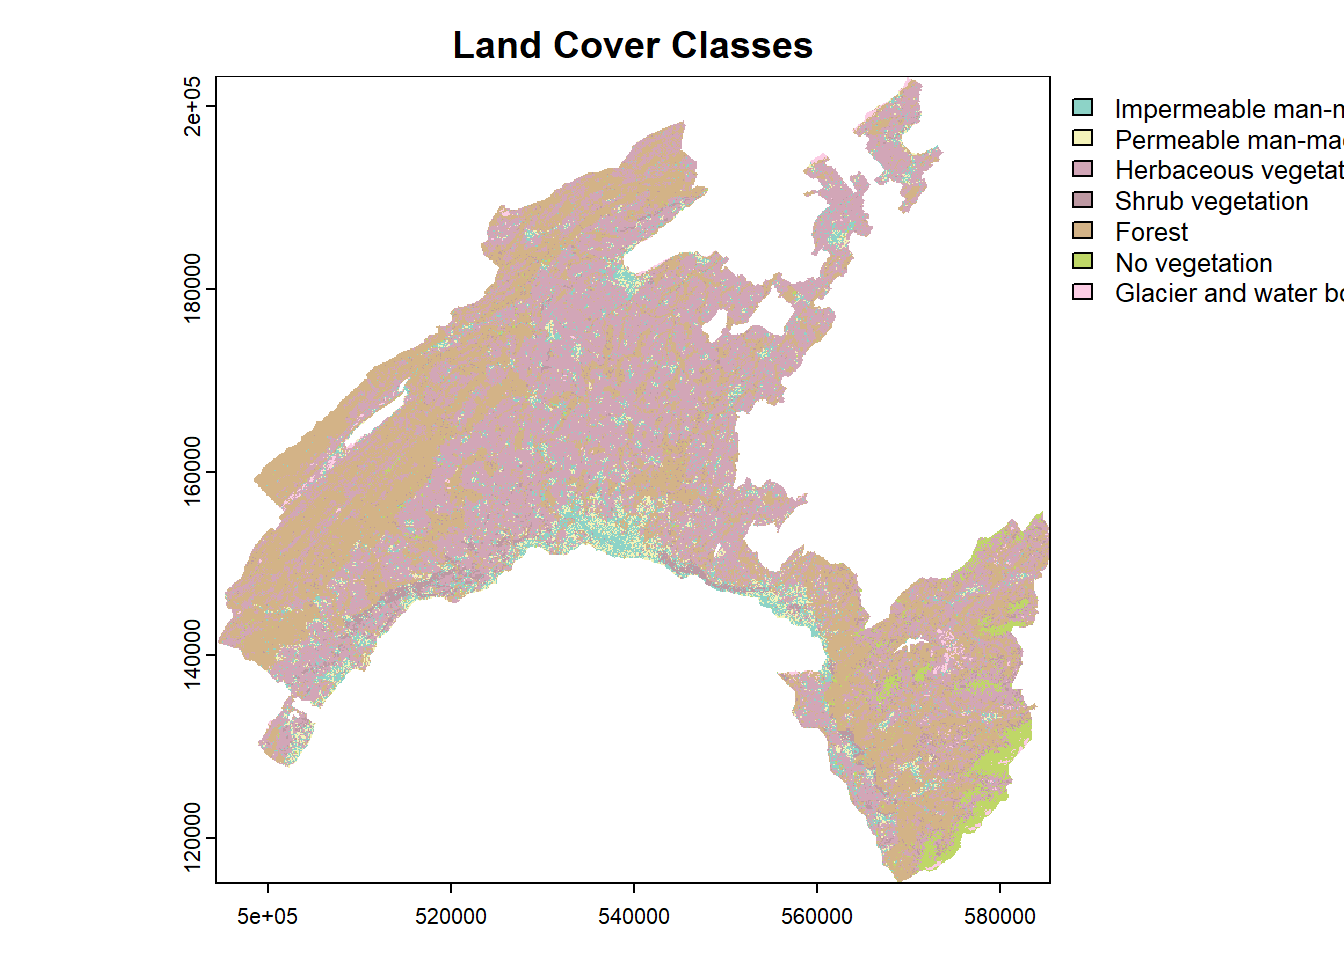
\includegraphics{02-RGIS_files/figure-latex/landCover-map-2} \end{center}

\subsection{Further Reading}\label{further-reading}

This chapter aims to provide an overview of the main functionalities integrated into the R packages \textbf{sf} and \textbf{terra} for vector and raster data manipulation. For more in-depth knowledge and understanding, you can refer to the following documentation:

\begin{itemize}
\item
  \texttt{sf} \href{https://r-spatial.github.io/sf/index.html}{Simple Features for R}
\item
  \texttt{terra} \href{https://rspatial.github.io/terra/index.html}{R~package for spatial data analysis}
\item
  \texttt{dplyr} \href{https://dplyr.tidyverse.org/index.html}{Solves most common data manipulation challenges}
\end{itemize}

\section{Geographically Weighted Summary Statistics for Geosciences}\label{gwss}

Geographically Weighted Summary Statistics (GWSS) represent an advanced analytical approach in geosciences, allowing researchers to explore spatial variations in data across a geographical landscape. Unlike traditional summary statistics that provide a single, overall summary measure -- like mean, median, or standard deviation -- for the entire dataset (i.e., globally), GWSS techniques calculate these measures locally, reflecting the unique characteristics and variations at different spatial locations. This method is particularly valuable in geosciences, where spatial heterogeneity often plays a critical role.

\subsection{GWSS for natural hazards assessment}\label{gwss-for-natural-hazards-assessment}

In the assessment of natural hazards -- like forest fires, earthquakes, flooding, or landslides -- identifying hotspots is a first step in prioritizing areas for risk management and mitigation strategies. This process helps in understanding which regions are most vulnerable, allowing for the allocation of resources, implementation of protective measures, and development of emergency response plans to reduce the potential impact on communities and infrastructure.

Although spatio-temporal inventories of natural hazards are made available, extracting meaningful insights about their distribution patterns remains challenging when relying solely on the examination of mapped event locations. To address this, Geographically Weighted Summary Statistics (GWSS) can be utilized. GWSS assumes that the spatial distribution of the single occurrences within a certain area exhibits geographic trends, and calculates local statistics to reveal these patterns more clearly. This approach provides valuable insights for effective management and prevention strategies.

As case study, in the present computing lab we compute the GW local means, the GW local standard deviation and the GW localized skewness of wildfires -- made available as mapped burned areas dataset -- in continental Portugal, registered in the period 1990-2013. This application is inspired by the work of \citep{tonini_evolution_2017}

\subsubsection{The overall methodology}\label{the-overall-methodology}

\textbf{Summary statistics} include a number of measures that can be used to summarize a set of observations, the most important of which are measures of central tendency (arithmetic mean, median, mode) and measures of dispersion around the mean (variance, standard deviation). In addition, measures of skewness and kurtosis are descriptors of the shape of the probability distribution function, the former indicating the asymmetry and the latter the peakedness/tailedness of the curve.

For geoenvironmental processes, these global statistical descriptors may vary from one region to another, as their values may be affected by local environmental and socio-economic factors. In this case, an appropriately localized calibration can provide a better description of the observed values. One way to achieve this goal is to weight the above statistical measures for a given quantitative variable based on their geographical location.

For the comoputation we introduce here the method proposed by \citep{brunsdon_geographically_2002} and implemented in the function \texttt{GWSS} presented in the R package GWmodel \citep{lu_gwmodel_2014, Gollini_2015}.

The evaluation of geographically weighted summary statistics is obtained by computing a summary for a small area around each geolocalized punctual observation, by using the Kernel Density Estimation technique (KDE) \citep{brunsdon_estimating_1995}. KDE is estimated at each point, taking into account the influence of the points falling within an area, with increasing weight towards the center, corresponding to the point location. A surface summary statistic is thus obtained.

\subsubsection{Forest fires dataset}\label{forest-fires-dataset}

Forest fires inventories indicating the location, the starting date and other related variables, such as the cause of ignition and the size of the area burned, are broadly available with a different degree of accuracy in different countries.

In the present study, we consider the \href{https://www.icnf.pt/florestas/gfr/gfrgestaoinformacao/dfciinformacaocartografica}{Portuguese National Mapping Burnt Areas} dataset , freely available from the website of the \href{https://www.icnf.pt/}{Institute for the Conservation of Nature and Forests}. This is a long spatio-temporal dataset resulting from the processing of satellite images acquired once a year at the end of the summer season. Row data consists of records of observed fire scars. The burned areas were estimated by using image classification techniques, then compared with ground data to resolve the discrepancies. Polygons have been converted into a point vector dataset, where each point represent the centroid of the burned areas, while the size of the burned areas and the starting date of the fires events are given as attributes.

In this work, for consistency reasons, we consider only fires occurred between 1990 and 2013, and with a burned area above 5 hectares.

\subsection{Computing lab: GWSS}\label{computing-lab-gwss}

\subsubsection{Load the libraries}\label{load-the-libraries}

First you have to load the following libraries:

\begin{itemize}
\tightlist
\item
  \emph{splancs}: for display and analysis of spatial point pattern data
\item
  \emph{GWmodel}: techniques from a particular branch of spatial statistics, termed geographically-weighted (GW) models
\item
  \emph{sf}: support for simple features, a standardized way to encode spatial vector data
\item
  \emph{ggplot2}: a system for `declaratively' creating graphics
\item
  \emph{sp}: classes and methods for spatial data
\end{itemize}

\begin{Shaded}
\begin{Highlighting}[]
\FunctionTok{library}\NormalTok{(splancs)}
\FunctionTok{library}\NormalTok{(GWmodel)}
\FunctionTok{library}\NormalTok{(sf)}
\FunctionTok{library}\NormalTok{(ggplot2)}
\FunctionTok{library}\NormalTok{(sp)}

\NormalTok{(}\FunctionTok{.packages}\NormalTok{())}
\end{Highlighting}
\end{Shaded}

\subsubsection{Import the forest fire dataset}\label{import-the-forest-fire-dataset}

In this section you will load the geodata representing the forest fires inventory for events occurred in the continental Portuguese area in the period 1990-2013. You will also load the boundaries of the study area. You will start by exploring the datasets using mainly visual tools (plotting and histogram).

\begin{Shaded}
\begin{Highlighting}[]
\CommentTok{\# Import Portugal boundary }
\NormalTok{Portugal }\OtherTok{\textless{}{-}} \FunctionTok{st\_read}\NormalTok{(}\StringTok{"data/GWSS/Area\_Portugal.shp"}\NormalTok{)}

\CommentTok{\# Import the Portuguese forest fires dataset for the entire Portuguese area.}
\NormalTok{FFPorto}\OtherTok{\textless{}{-}}\FunctionTok{st\_read}\NormalTok{(}\StringTok{"data/GWSS/FF\_Portugal.shp"}\NormalTok{)}
\end{Highlighting}
\end{Shaded}

You can explore the dataset by using different tools for \textbf{exploratory data analyses}. You will start by visualizing the databases (i.e., the attribute table). Than you can plot the histogram of events distribution based on the variable \emph{``Area\_ha''} (i.e., the size in hectares of the burned area). Since this is a power low distribution, for a better understanding it is recommended to transform the data using a logarithmic scale. Computiong \emph{log10} you can easily evaluate the frequency distribution of the burned areas.

\begin{Shaded}
\begin{Highlighting}[]
\CommentTok{\# Show the attribute table (first 10 rows) }
\NormalTok{FFPorto }
\end{Highlighting}
\end{Shaded}

\begin{verbatim}
## Simple feature collection with 27273 features and 4 fields
## Geometry type: POINT
## Dimension:     XY
## Bounding box:  xmin: 82126.92 ymin: 7083.529 xmax: 361492.2 ymax: 573192.5
## Projected CRS: Lisboa_Hayford_Gauss_IGeoE
## First 10 features:
##    Year Area_ha        X        Y                  geometry
## 1  1990   5.000 275224.0 525501.4   POINT (275224 525501.4)
## 2  1990   5.000 235278.0 452412.9   POINT (235278 452412.9)
## 3  1990   5.000 200628.8 491568.2 POINT (200628.8 491568.2)
## 4  1990   5.000 120687.8 228816.9 POINT (120687.8 228816.9)
## 5  1990   5.031 207183.9 498247.7 POINT (207183.9 498247.7)
## 6  1990   5.031 162730.0 488388.8   POINT (162730 488388.8)
## 7  1990   5.031 250545.2 532563.7 POINT (250545.2 532563.7)
## 8  1990   5.031 268013.3 356110.4 POINT (268013.3 356110.4)
## 9  1990   5.033 222095.7 543059.9 POINT (222095.7 543059.9)
## 10 1990   5.044 207265.7 377657.8 POINT (207265.7 377657.8)
\end{verbatim}

\begin{Shaded}
\begin{Highlighting}[]
\CommentTok{\# Open the attribute table in a new tab }
\FunctionTok{View}\NormalTok{(FFPorto) }

\CommentTok{\# Summary statistics of all of the attributes associated with this dataset}
\FunctionTok{summary}\NormalTok{(FFPorto}\SpecialCharTok{$}\NormalTok{Area\_ha)}
\end{Highlighting}
\end{Shaded}

\begin{verbatim}
##     Min.  1st Qu.   Median     Mean  3rd Qu.     Max. 
##     5.00     9.78    20.41   107.14    56.07 66070.63
\end{verbatim}

\begin{Shaded}
\begin{Highlighting}[]
\CommentTok{\# Histogram of the forest fires distribution by year }
\FunctionTok{hist}\NormalTok{(FFPorto}\SpecialCharTok{$}\NormalTok{Year, }\AttributeTok{breaks =} \FunctionTok{unique}\NormalTok{(FFPorto}\SpecialCharTok{$}\NormalTok{Year), }\AttributeTok{xlim=}\FunctionTok{c}\NormalTok{(}\DecValTok{1990}\NormalTok{,}\DecValTok{2015}\NormalTok{), }\AttributeTok{ylim=}\FunctionTok{c}\NormalTok{(}\DecValTok{0}\NormalTok{,}\DecValTok{2500}\NormalTok{))}
\end{Highlighting}
\end{Shaded}

\begin{center}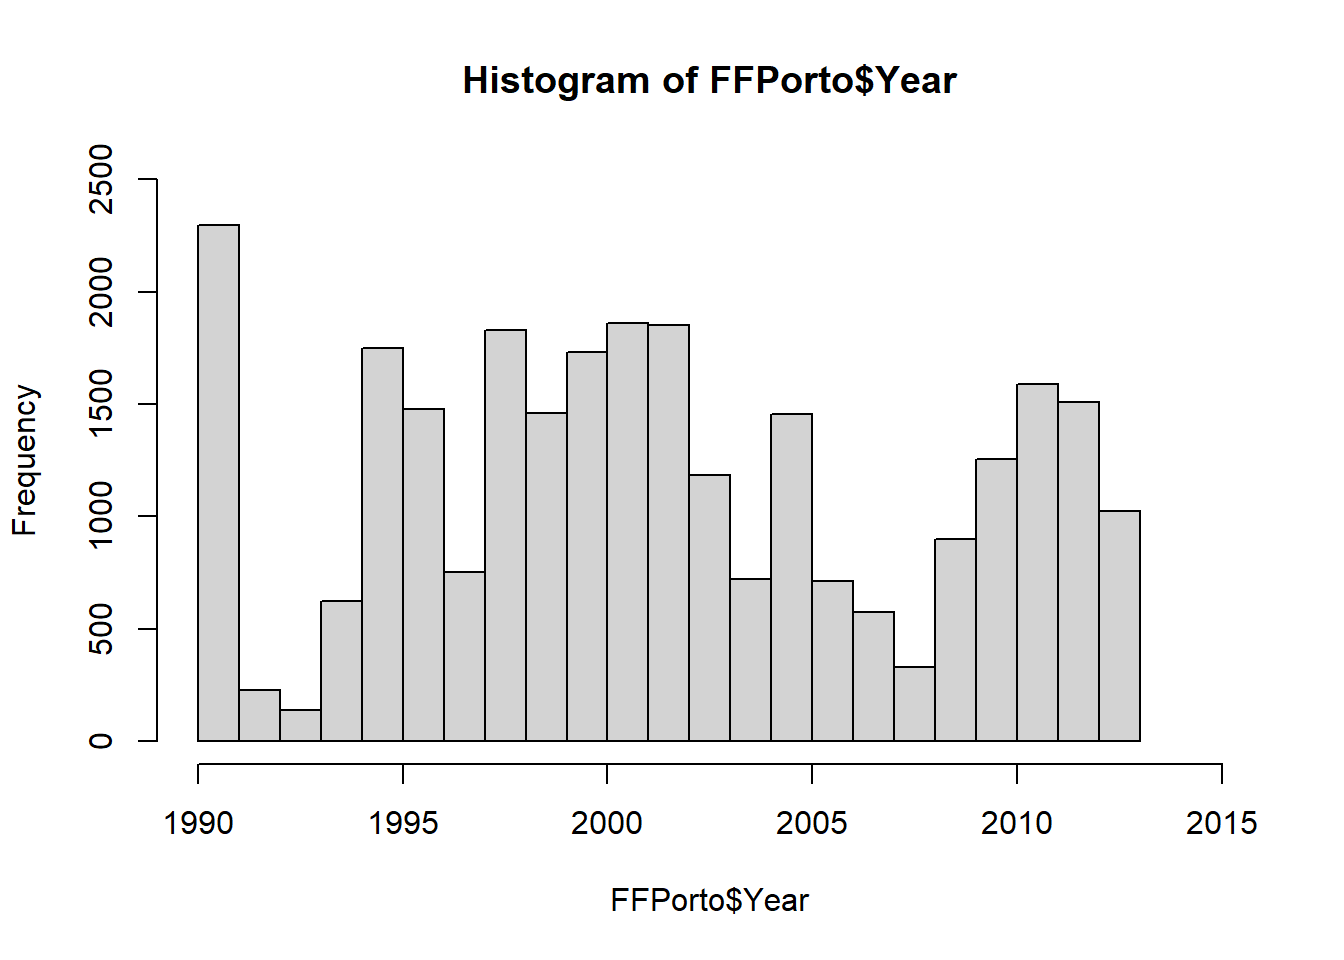
\includegraphics{03-GWSS_files/figure-latex/histo-FF-1} \end{center}

\begin{Shaded}
\begin{Highlighting}[]
\CommentTok{\# Histogram of the forest fires distribution by burned area }


\FunctionTok{hist}\NormalTok{(FFPorto}\SpecialCharTok{$}\NormalTok{Area\_ha) }\CommentTok{\#power low disrtibution}
\end{Highlighting}
\end{Shaded}

\begin{center}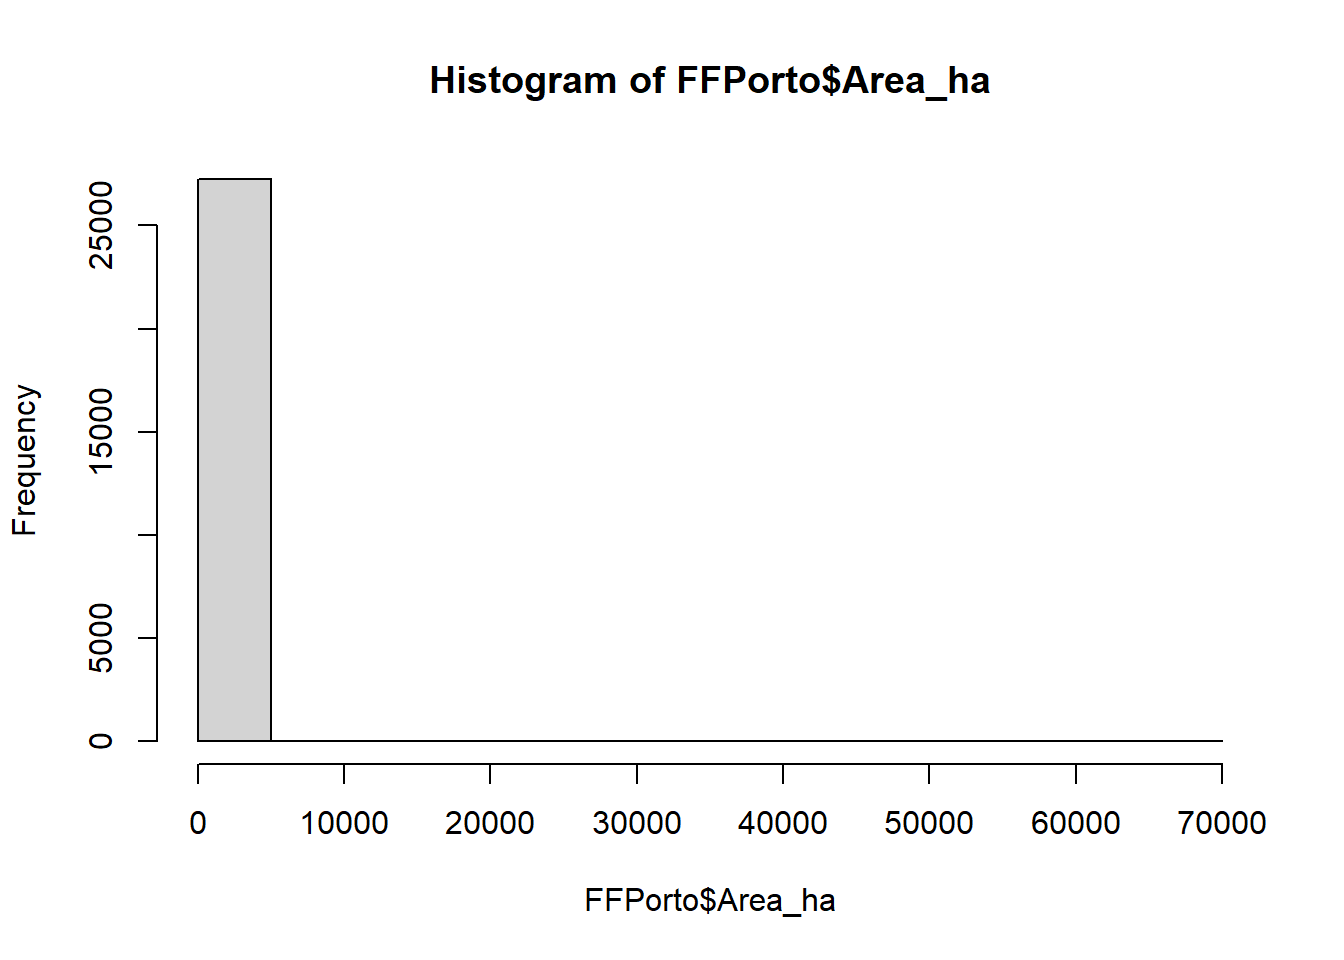
\includegraphics{03-GWSS_files/figure-latex/histo-FF-2} \end{center}

\begin{Shaded}
\begin{Highlighting}[]
\FunctionTok{hist}\NormalTok{(}\FunctionTok{log10}\NormalTok{(FFPorto}\SpecialCharTok{$}\NormalTok{Area\_ha)) }\CommentTok{\#log transformation}
\end{Highlighting}
\end{Shaded}

\begin{center}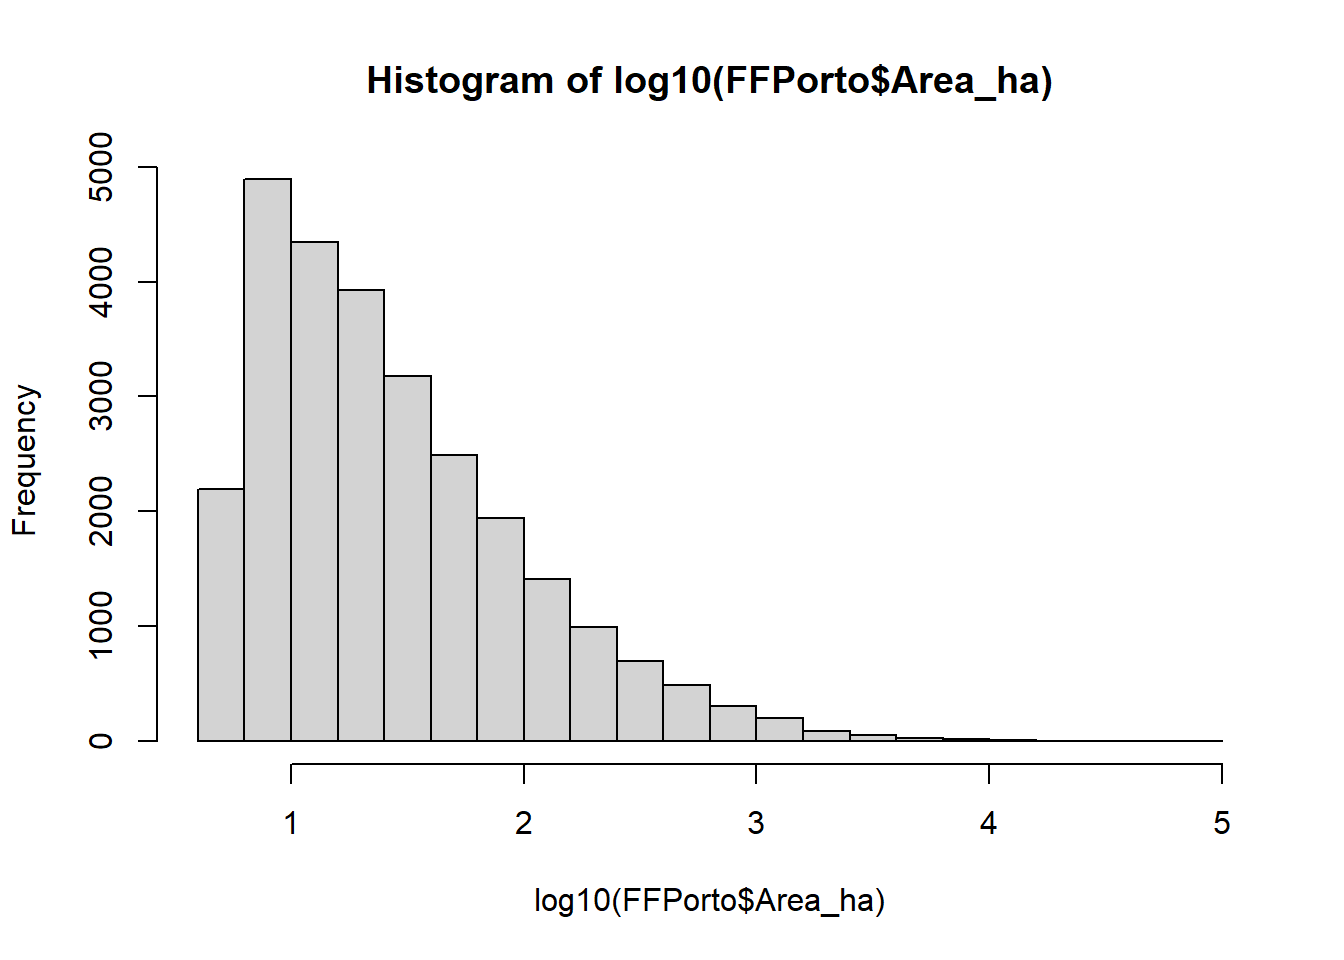
\includegraphics{03-GWSS_files/figure-latex/histo-FF-3} \end{center}

\subsubsection{Forest fires spatial distribution}\label{forest-fires-spatial-distribution}

For a better understanding of the phenomenon, you can group the events according to the size of the burned areas. Base on a mix of empirical experience and the frequency distribution of forest fires presented in our dataset, by area, the following three classes can be defined:

\begin{itemize}
\tightlist
\item
  \emph{Small fires:} less than 15 ha
\item
  \emph{Medium fires:} between 15 ha and 100 ha
\item
  \emph{Large fires:} bigger than 100 ha
\end{itemize}

Plotting the forest fire events using different colors, based on the size of the burned areas, can simplify the understanding of their pattern distribution, knowing that fires of different size have normally different drivers.

\begin{center}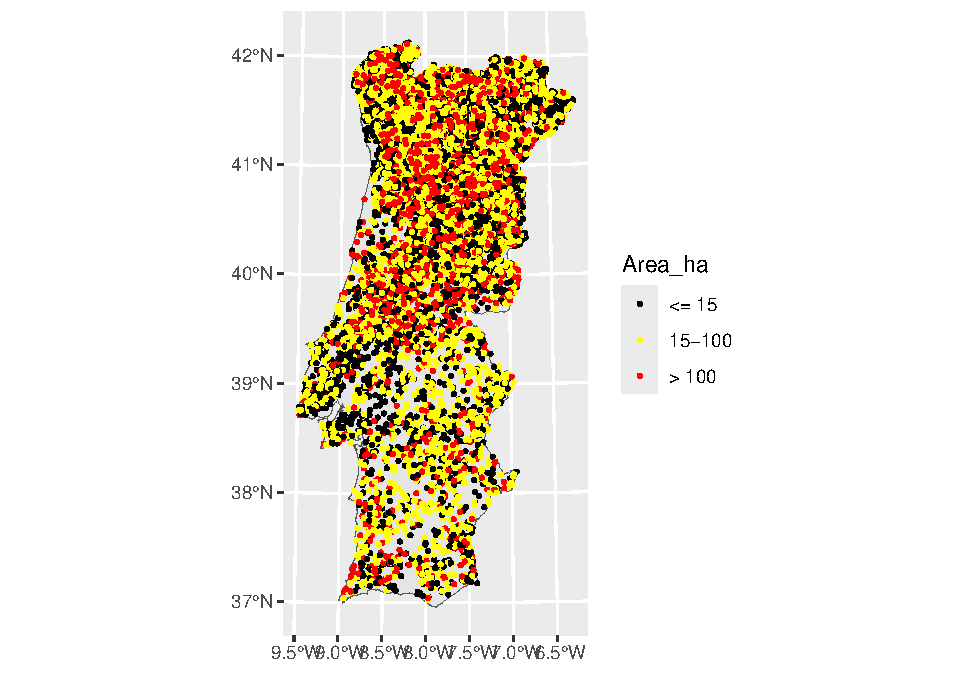
\includegraphics{03-GWSS_files/figure-latex/plot-all-fires-1} \end{center}

\subsubsection{Compute the GWSS}\label{compute-the-gwss}

From the exploratory data analysis performed above, it seems that a simple plotting of the forest fires events based on their spatial distribution, even if classified based on their size, can not really help to understand their spatial behaviors. This is because we face to a huge number of events and the variable that we are using to characterize them -- the size of the burned area, in our case -- is very heterogeneous. To this aim, we can compute basic and robust GWSS and plot the data accordingly.

The GWSS includes \emph{geographically weighted means}, \emph{standard deviations} and the \emph{skweness}. As you can see from the R Documentation -- command: \texttt{help(gwss)} -- same data manipulations are necessary to transform the forest fires dataset into a compatible data frame format.

\begin{Shaded}
\begin{Highlighting}[]
\CommentTok{\# Transform inputs data into a spatial points data frame}
\NormalTok{FFdf}\OtherTok{\textless{}{-}}\FunctionTok{data.frame}\NormalTok{(}\AttributeTok{X=}\NormalTok{FFPorto}\SpecialCharTok{$}\NormalTok{X, }\AttributeTok{Y=}\NormalTok{FFPorto}\SpecialCharTok{$}\NormalTok{Y, }\AttributeTok{Area=}\NormalTok{FFPorto}\SpecialCharTok{$}\NormalTok{Area\_ha)}
\NormalTok{FFspdf}\OtherTok{\textless{}{-}}\FunctionTok{SpatialPointsDataFrame}\NormalTok{(FFdf[,}\DecValTok{1}\SpecialCharTok{:}\DecValTok{2}\NormalTok{], FFdf)}
\FunctionTok{str}\NormalTok{(FFspdf)}
\end{Highlighting}
\end{Shaded}

\textbf{GWSS parameters}:

\begin{itemize}
\tightlist
\item
  we summarize the data based on the size of the burned area (\texttt{vars})
\item
  we use here an adaptive kernel where the bandwidth (\texttt{bw}) corresponds to the number (100 in this case) of nearest neighbors (i.e.~\texttt{adaptive} distance)
\item
  we keep the default values for the other parameters
\end{itemize}

\begin{Shaded}
\begin{Highlighting}[]
\CommentTok{\# Run gwss: this operation can take several minutes...be patient!}

\CommentTok{\# While waiting, you can look at gwss R Documentation:}
\FunctionTok{help}\NormalTok{(gwss)}

\NormalTok{FFgwss }\OtherTok{\textless{}{-}} \FunctionTok{gwss}\NormalTok{(FFspdf,}\AttributeTok{vars=}\NormalTok{(}\StringTok{"Area"}\NormalTok{),}\AttributeTok{adaptive=}\ConstantTok{TRUE}\NormalTok{, }\AttributeTok{bw=}\DecValTok{100}\NormalTok{)}
\end{Highlighting}
\end{Shaded}

\subsubsection{Look at the results}\label{look-at-the-results}

The resulting object (\texttt{FFgwss}) has a number of components. The most important one is the spatial data frame containing the results of local summary statistics for each data point location, stored in \texttt{FFgwss\$SDF} (that is a spatial data frame).

\begin{Shaded}
\begin{Highlighting}[]
\CommentTok{\# Inspect the output }
\NormalTok{FFgwss}
\end{Highlighting}
\end{Shaded}

\begin{verbatim}
##    ***********************************************************************
##    *                       Package   GWmodel                             *
##    ***********************************************************************
## 
##    ***********************Calibration information*************************
## 
##    Local summary statistics calculated for variables:
##     Area
##    Number of summary points: 27273
##    Kernel function: bisquare 
##    Summary points: the same locations as observations are used.
##    Adaptive bandwidth: 100 (number of nearest neighbours)
##    Distance metric: Euclidean distance metric is used.
## 
##    ************************Local Summary Statistics:**********************
##    Summary information for Local means:
## Area_LM 
##       Min.    1st Qu.     Median    3rd Qu.       Max. 
##   10.97782   42.54450   70.89374  120.67898 2300.80424 
##    Summary information for local standard deviation :
## Area_LSD 
##         Min.      1st Qu.       Median      3rd Qu.         Max. 
##     6.856477    74.310044   149.714657   292.508111 11280.136286 
##    Summary information for local variance :
## Area_LVar 
##         Min.      1st Qu.       Median      3rd Qu.         Max. 
## 4.701127e+01 5.521983e+03 2.241448e+04 8.556100e+04 1.272415e+08 
##    Summary information for Local skewness:
## Area_LSKe 
##       Min.    1st Qu.     Median    3rd Qu.       Max. 
##   0.829069   3.178626   4.373189   6.076042 192.906106 
##    Summary information for localized coefficient of variation:
## Area_LCV 
##       Min.    1st Qu.     Median    3rd Qu.       Max. 
##  0.6245756  1.5756289  2.0240543  2.6604986 16.0254231 
## 
##    ************************************************************************
\end{verbatim}

\begin{Shaded}
\begin{Highlighting}[]
\CommentTok{\# Display the first 6 rows}
\FunctionTok{head}\NormalTok{(FFgwss}\SpecialCharTok{$}\NormalTok{SDF) }
\end{Highlighting}
\end{Shaded}

\begin{verbatim}
##            coordinates  Area_LM  Area_LSD  Area_LVar Area_LSKe  Area_LCV
## 1   (275224, 525501.4) 56.46496 127.16616 16171.2316  4.612383 2.2521253
## 2   (235278, 452412.9) 89.17704 196.51574 38618.4344  4.384154 2.2036585
## 3 (200628.8, 491568.2) 25.64396  25.02941   626.4712  2.851515 0.9760351
## 4 (120687.8, 228816.9) 16.37948  17.85761   318.8941  3.435847 1.0902427
## 5 (207183.9, 498247.7) 46.54590  84.45980  7133.4579  4.465928 1.8145489
## 6   (162730, 488388.8) 28.54313  35.14293  1235.0258  2.400911 1.2312221
\end{verbatim}

\subsubsection{GWSS maps}\label{gwss-maps}

To produce a map of the local geographically weighted summary statistic of your choice, firstly we need to enter a small R function definition. This is just a short R program to draw a map: you can think of it as a command that tells R how to draw a map (from \citep{chris_brunsdon_geographically_2015} ). The advantage of defining a function is that the entire map can now be drawn using a single command for each variable, rather than having to repeat those steps each time. To define the intervals for the classification, we use Jenks natural breaks classification method (\texttt{style="fisher"}).

\begin{Shaded}
\begin{Highlighting}[]
\FunctionTok{library}\NormalTok{(RColorBrewer) }\CommentTok{\#a useful tool for designing map color palettes.}
\FunctionTok{library}\NormalTok{(classInt) }\CommentTok{\#to define class intervals}

\CommentTok{\# The function definition to draw the map:}

\NormalTok{quick.map }\OtherTok{\textless{}{-}} \ControlFlowTok{function}\NormalTok{(spdf,var,legend.title,main.title) \{}
\NormalTok{  x }\OtherTok{\textless{}{-}}\NormalTok{ spdf}\SpecialCharTok{@}\NormalTok{data[,var]}
\NormalTok{  int }\OtherTok{\textless{}{-}} \FunctionTok{classIntervals}\NormalTok{(x, }\AttributeTok{n=}\DecValTok{5}\NormalTok{, }\AttributeTok{style=}\StringTok{"fisher"}\NormalTok{)}
\NormalTok{  cut.vals}\OtherTok{\textless{}{-}}\NormalTok{int}\SpecialCharTok{$}\NormalTok{brks}
\NormalTok{  x.cut }\OtherTok{\textless{}{-}} \FunctionTok{cut}\NormalTok{(x,cut.vals)}
\NormalTok{  cut.levels }\OtherTok{\textless{}{-}} \FunctionTok{levels}\NormalTok{(x.cut)}
\NormalTok{  cut.band }\OtherTok{\textless{}{-}} \FunctionTok{match}\NormalTok{(x.cut,cut.levels)}
\NormalTok{  colors }\OtherTok{\textless{}{-}} \FunctionTok{rev}\NormalTok{(}\FunctionTok{brewer.pal}\NormalTok{(}\FunctionTok{length}\NormalTok{(cut.levels), }\StringTok{"RdYlGn"}\NormalTok{))}
  \FunctionTok{par}\NormalTok{(}\AttributeTok{mar=}\FunctionTok{c}\NormalTok{(}\DecValTok{1}\NormalTok{,}\DecValTok{1}\NormalTok{,}\DecValTok{1}\NormalTok{,}\DecValTok{1}\NormalTok{))}
  \FunctionTok{plot}\NormalTok{(Portugal}\SpecialCharTok{$}\NormalTok{geometry,}\AttributeTok{col=}\StringTok{\textquotesingle{}lightgrey\textquotesingle{}}\NormalTok{)}
  \FunctionTok{title}\NormalTok{(main.title)}
  \FunctionTok{plot}\NormalTok{(spdf,}\AttributeTok{add=}\ConstantTok{TRUE}\NormalTok{,}\AttributeTok{col=}\NormalTok{colors[cut.band],}\AttributeTok{pch=}\DecValTok{16}\NormalTok{, }\AttributeTok{cex=}\FloatTok{0.5}\NormalTok{)}
  \FunctionTok{legend}\NormalTok{(}\StringTok{"bottomright"}\NormalTok{,cut.levels,}\AttributeTok{col=}\NormalTok{colors,}\AttributeTok{pch=}\DecValTok{16}\NormalTok{,}\AttributeTok{bty=}\StringTok{"n"}\NormalTok{,}\AttributeTok{title=}\NormalTok{legend.title)}
\NormalTok{  \}}

\CommentTok{\# Call the function to display the maps of the Local Mean (LM), Local Standard Deviation(LS), and Local Skweness (LSKe)}

\FunctionTok{par}\NormalTok{(}\AttributeTok{mfrow=}\FunctionTok{c}\NormalTok{(}\DecValTok{1}\NormalTok{,}\DecValTok{3}\NormalTok{))}
\FunctionTok{quick.map}\NormalTok{(FFgwss}\SpecialCharTok{$}\NormalTok{SDF, }\StringTok{"Area\_LM"}\NormalTok{, }\StringTok{"Area (ha)"}\NormalTok{, }\StringTok{"GW{-}Mean"}\NormalTok{)}
\FunctionTok{quick.map}\NormalTok{(FFgwss}\SpecialCharTok{$}\NormalTok{SDF, }\StringTok{"Area\_LSD"}\NormalTok{, }\StringTok{"Area (ha)"}\NormalTok{, }\StringTok{"GW{-}Standard Deviation"}\NormalTok{)}
\FunctionTok{quick.map}\NormalTok{(FFgwss}\SpecialCharTok{$}\NormalTok{SDF, }\StringTok{"Area\_LSKe"}\NormalTok{, }\StringTok{"Area (ha)"}\NormalTok{, }\StringTok{"GW{-}Skewness"}\NormalTok{)}
\end{Highlighting}
\end{Shaded}

\begin{center}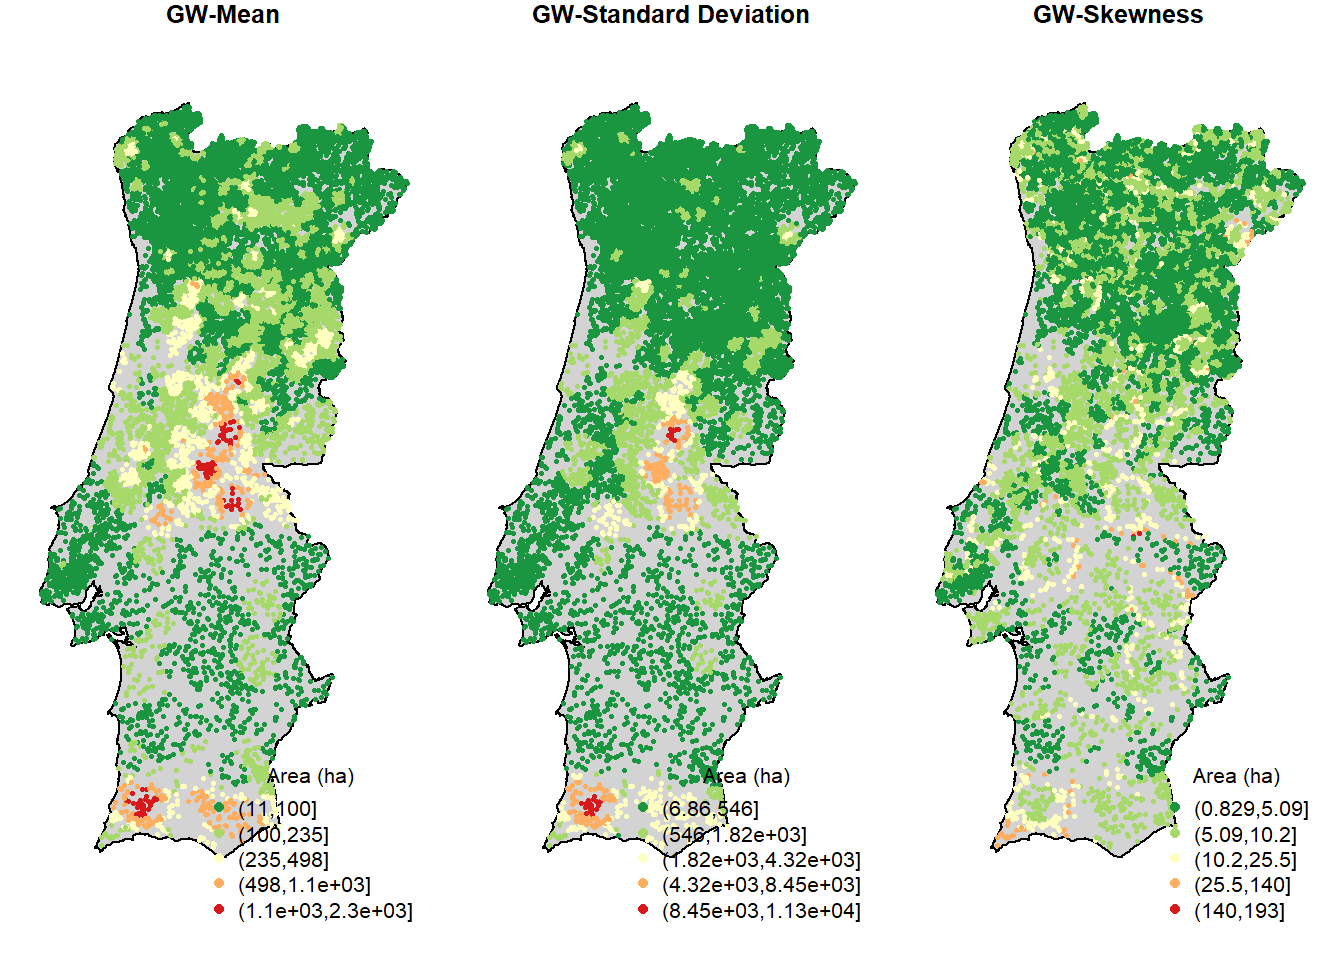
\includegraphics{03-GWSS_files/figure-latex/gwss-maps-1} \end{center}

\subsection{Conclusions and further analyses}\label{conclusions-and-further-analyses}

This practical computer lab allowed you to familiarize with GWSS, by the proposed application about geographically weighted summary statistics. This approach allowed us to explore how the average burned area vary locally through Continental Portugal in the period 1990-2013.

The global Geographically Weighted (GW) mean informs us about the local average value of the burned area, based of the neighboring events occurred in a given period. Similarly, the GW standard deviation allows to inspect the extent to which the size of the burned area spread around this mean. Finally, the GW skewness measures the symmetry of the distribution: a positively skewed distribution means that there is a high number of observations with mean value lower that the median; and the contrary for a negatively skewed distribution.

To ensure that everything is perfectly clear, we propose you to answer the following questions. You can find the correct responses in the reference paper \citep{tonini_evolution_2017}.

\begin{enumerate}
\def\labelenumi{\arabic{enumi})}
\item
  Describe the pattern distribution of the GW-Mean for burned area in Portugal during the investigated periods.
\item
  Does the GW-Standard Deviation follows the same pattern? How can you interpret these two pattern distributions in terms of burned area and their characterization?
\item
  The GW-Skewness has positive values everywhere: what does it means? What do these values suggest to be the distribution of the burned areas, in terms of their size, around the local mean?
\item
  Which can be other applications of GWSS in geosciences data? In other words, can you imagine other geo-environmental dataset that can be analysed using GWSS?
\item
  Finally, you can play with the code and try to run it using a different numbers of nearest neighbors (\texttt{bw=x}) and compare the results.
\end{enumerate}

\section{Spatio-Temporal Cluster Analysis of GeoEnvironmental Processes}\label{kde}

Spatio-temporal cluster analysis (ST clustering) is a powerful tool used to identify patterns and relationships in data that vary across both space and time.
In the context of geoenvironmental processes, this type of analysis can helps in understanding how environmental phenomena --- such as wildfires, landslides, or flood events --- are distributed geographically and how they evolve over time.
By detecting clusters, researchers can uncover hotspots, assess trends, and identify potential triggers or influencing factors, leading to more informed decision-making and targeted interventions in environmental management.

\subsection{ST clustering for fire management}\label{st-clustering-for-fire-management}

The configuration of forest fires across space and time presents a complex pattern which significantly affects the forest environment and adjacent human developments.
Statistical techniques designed for spatio-temporal random point processes can be utilized to identify a structure, recognize hot-spots and vulnerable areas, and address policy makers to prevention and forecasting measures.

In this practical computing lab we consider the same case study as in the ``Geographically Weighted Summary Statistics'' lab.
The main objective is to reveal if space and time act independently or whether neighboring events are also closer in time, interacting to generate ST clusters.
The attribute that we will consider to achieve this goal is the starting date of fires events.
To account for the different geographical distribution of fires in Portugal, events occurred in the Norther and Southern areas will be modeled separately.

For more details about the input dataset, please refer to the GWSS lab documentation.

\subsection{Clustering methods}\label{clustering-methods}

To detect spatio-temporal clusters of forest fires, we will use the following statistical methods:

\begin{enumerate}
\def\labelenumi{(\arabic{enumi})}
\item
  The \textbf{Ripley's K- function} to test the space-time interaction and the spatial attraction/independency between fires of different size.
\item
  The \textbf{Kernel Density Estimator} allowing elaborating smoothed density surfaces representing hotspots.
\end{enumerate}

We provide below a short description for both these methods.
More details can be found in \citep{tonini_evolution_2017}, the paper which inspired the present lab.

\subsubsection{Ripley's K-function}\label{ripleys-k-function}

The Ripley's K-function allows inferring about the spatial randomness of mapped punctual events \citep{ripley1977modelling}.
It is largely applied in geosciences to analyse the pattern distribution of a spatial point process.
The original spatial univariate K-function \(K(s)\) is defined as the ratio between the expected number \(E\) of point events falling at a certain distance \(r\) from an arbitrary event and the intensity \(\lambda\) of the spatial point process, this last corresponding to the average number of points per unit area.

Under complete spatial randomness, which assumes the independence among the events, \(K(s)\) is equal to the area of the circle around the target event at any distance's value.
It follows that events are spatially clustered within the range of distances at which \(K(s)\) assumes vales higher than this area, while they are spatially dispersed for lower values.
The temporal K-function \(K(t)\) is defined in the same way as for the spatial case, with the time-based intensity and the time length replacing the spatial distance.

\paragraph{Spatio-temporal interaction}\label{spatio-temporal-interaction}

The space-time K-function \(K(s,t)\) can be considered as a bivariate function where space and time represent the two variables of the equation.
It is defined as the number of further events occurring within a distance \(r\) and time \(t\) from an arbitrary event.

If there is no space-time interaction, \(K(s,t)\) is equal to the product of the purely spatial and purely temporal K-function.
Inversely, if space and time interact generating clusters, the difference \(D(s,t)\) between these two values is positive, where:

\[D(s,t)=K(s,t)-K(s)*K(t)\]

Thus, we can use the perspective 3D-plot of the function \(D(s,t)\) to obtain a first diagnostic of space-time clustering: positive values indicate an interaction between these two variables at a well-detectable spatio-temporal scale.

\subsubsection{Kernel density estimator}\label{kernel-density-estimator}

The Kernel Density Estimator (KDE) is a non-parametric descriptor tool widely applied in geosciences to elaborate smoothed density surfaces from spatial variables.
A kernel function \(K\) allows weighing up the contribution of each event, based on the relative distance of neighborings to the target.
The parameter \(h\), called bandwidth, controls the smoothness of the estimated kernel density.
Finally, the kernel density function \(f_h(x)\) is estimated by summing all the kernel functions \(K\) computed at each point location \(x\) and dividing the result by the total number of events (\(n\)): \[f_h(x) = \frac{1}{nh}\sum_{i=j}^{n}K(\frac{x-x_i}{h})\]

The time extension of the kernel density estimator allows to compute the three-dimensional kernel density estimator which includes the spatio-temporal dimensions\citep{nakaya_visualising_2010}.

In the present case study we apply a quadratic weighting kernel function, which is an approximation to the Gaussian kernel.
Regarding the bandwidth's value, we propose to consider the results of the spatio-temporal K-function as an indicator.
Indeed, the distance values showing a maximum cluster behavior over the displayed perspective \(D(s,t)\) plot can be attributed to the \(h\)-value, minimizing the problem of under- or over-smoothing due to an arbitrary choice of the bandwidth.

\subsection{Computing lab: ST clustering}\label{computing-lab-st-clustering}

\subsubsection{Load the libraries}\label{load-the-libraries-1}

Fist you have to load the following libraries:

\begin{itemize}
\tightlist
\item
  \emph{splancs}: for display and analysis of spatial point pattern data
\item
  \emph{sf}: support for simple features, a standardized way to encode spatial vector data
\item
  \emph{ggplot2}: s system for `declaratively' creating graphics
\item
  \emph{sp}: classes and methods for spatial data
\item
  \emph{spatstat}: comprehensive open-source toolbox for analyzing Spatial Point Patterns
\end{itemize}

\begin{Shaded}
\begin{Highlighting}[]
\FunctionTok{library}\NormalTok{(splancs)}
\FunctionTok{library}\NormalTok{(spatstat)}
\FunctionTok{library}\NormalTok{(sf)}
\FunctionTok{library}\NormalTok{(ggplot2)}
\FunctionTok{library}\NormalTok{(sp)}

\NormalTok{(}\FunctionTok{.packages}\NormalTok{())}
\end{Highlighting}
\end{Shaded}

\subsubsection{Import the forest fire dataset}\label{import-the-forest-fire-dataset-1}

In this section you will load the geodata representing the dataset of the forest fires occurred in the continental Portuguese area in the period 1990-2013.
You will also load the boundaries of the study area.
You will start by exploring the datasets using mainly visual tools (plotting and histogram).

\begin{Shaded}
\begin{Highlighting}[]
\CommentTok{\# Import Portugal boundary }
\NormalTok{Portugal }\OtherTok{\textless{}{-}} \FunctionTok{st\_read}\NormalTok{(}\StringTok{"data/KDE/Portugal.shp"}\NormalTok{) }\CommentTok{\# entire area}

\NormalTok{PortN}\OtherTok{\textless{}{-}} \FunctionTok{st\_read}\NormalTok{(}\StringTok{"data/KDE/Porto\_North.shp"}\NormalTok{) }\CommentTok{\# northern area }
\NormalTok{PortS}\OtherTok{\textless{}{-}} \FunctionTok{st\_read}\NormalTok{(}\StringTok{"data/KDE/Porto\_South.shp"}\NormalTok{) }\CommentTok{\# southern}

\CommentTok{\# Import the forest fires dataset}

\NormalTok{FF}\OtherTok{\textless{}{-}}\FunctionTok{st\_read}\NormalTok{(}\StringTok{"data/KDE/ForestFires.shp"}\NormalTok{) }\CommentTok{\# entire area}
\NormalTok{FFN}\OtherTok{\textless{}{-}}\FunctionTok{st\_read}\NormalTok{(}\StringTok{"data/KDE/FF\_North.shp"}\NormalTok{) }\CommentTok{\# Northern area}
\NormalTok{FFS}\OtherTok{\textless{}{-}}\FunctionTok{st\_read}\NormalTok{(}\StringTok{"data/KDE/FF\_South.shp"}\NormalTok{) }\CommentTok{\# Southern area}

\CommentTok{\# Import the shapefile of the Tagus river}
\NormalTok{river}\OtherTok{\textless{}{-}}\FunctionTok{st\_read}\NormalTok{(}\StringTok{"data/KDE/Rio\_Tajo.shp"}\NormalTok{)}

\FunctionTok{summary}\NormalTok{(FF}\SpecialCharTok{$}\NormalTok{Area\_ha) }\CommentTok{\# summary statistics}
\FunctionTok{hist}\NormalTok{(FF}\SpecialCharTok{$}\NormalTok{Area\_ha)}
\end{Highlighting}
\end{Shaded}

\begin{center}\includegraphics{04-KDE_files/figure-latex/import-data-1} \end{center}

\begin{Shaded}
\begin{Highlighting}[]
\FunctionTok{hist}\NormalTok{(}\FunctionTok{log10}\NormalTok{(FF}\SpecialCharTok{$}\NormalTok{Area\_ha)) }\CommentTok{\# see the lab GWSS for more details }
\end{Highlighting}
\end{Shaded}

\begin{center}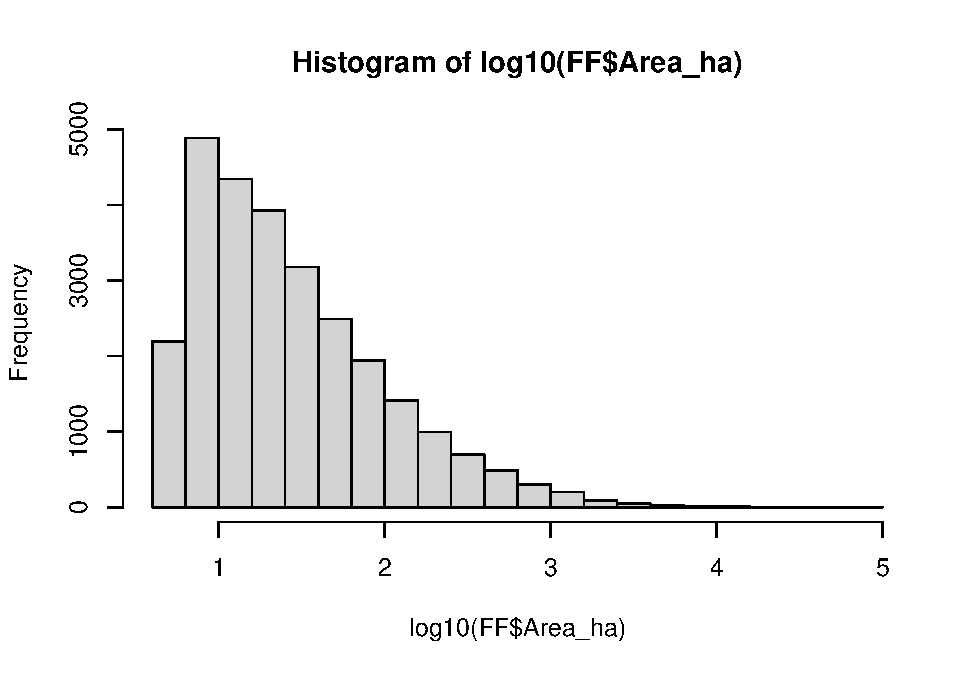
\includegraphics{04-KDE_files/figure-latex/import-data-2} \end{center}

For a better understanding of the phenomenon, events can be grouped according to the size of the burnt area and to their incidence in the northern and in the southern part of continental Portugal.

\subsubsection{Forest fires subsets based on the size of the burned area}\label{forest-fires-subsets-based-on-the-size-of-the-burned-area}

Remember that fires of different size can have been induced by different drivers.
Thus, in the following, we will investigate all the global cluster behavior of forest fires in Portugal considering the three subsets separately.

As you have seen in the lab GWSS, the following three classes can be defined based of the size of the burned area:

\begin{itemize}
\tightlist
\item
  \emph{Small fires:} less than 15 ha
\item
  \emph{Medium fires:} between 15 ha and 100 ha
\item
  \emph{Large fires:} bigger than 100 ha
\end{itemize}

\begin{Shaded}
\begin{Highlighting}[]
\NormalTok{SF}\OtherTok{=}\NormalTok{(}\FunctionTok{subset}\NormalTok{(FF, Area\_ha }\SpecialCharTok{\textless{}=}\DecValTok{15}\NormalTok{)) }\CommentTok{\#create a sub{-}set including only small fires. }

\FunctionTok{summary}\NormalTok{(SF)}
\end{Highlighting}
\end{Shaded}

\begin{verbatim}
##       Year         Area_ha             X                Y         
##  Min.   :1990   Min.   : 5.000   Min.   : 82761   Min.   :  7772  
##  1st Qu.:1997   1st Qu.: 6.624   1st Qu.:182973   1st Qu.:403849  
##  Median :2001   Median : 8.569   Median :213159   Median :472892  
##  Mean   :2002   Mean   : 9.041   Mean   :219789   Mean   :440692  
##  3rd Qu.:2008   3rd Qu.:11.219   3rd Qu.:259054   3rd Qu.:518384  
##  Max.   :2013   Max.   :15.000   Max.   :361492   Max.   :573193  
##           geometry    
##  POINT        :10902  
##  epsg:NA      :    0  
##  +proj=tmer...:    0  
##                       
##                       
## 
\end{verbatim}

\begin{Shaded}
\begin{Highlighting}[]
\CommentTok{\# This is to save the plot }
\NormalTok{pSF }\OtherTok{\textless{}{-}} \FunctionTok{ggplot}\NormalTok{ ()}\SpecialCharTok{+}
  \FunctionTok{geom\_sf}\NormalTok{(}\AttributeTok{data=}\NormalTok{Portugal)}\SpecialCharTok{+}
  \FunctionTok{geom\_sf}\NormalTok{(}\AttributeTok{data=}\NormalTok{SF, }\AttributeTok{size=}\FloatTok{0.5}\NormalTok{, }\AttributeTok{col=}\StringTok{"yellow"}\NormalTok{)}\SpecialCharTok{+}
 \FunctionTok{ggtitle}\NormalTok{(}\StringTok{"Small fires"}\NormalTok{) }\SpecialCharTok{+}
 \FunctionTok{coord\_sf}\NormalTok{()}
\end{Highlighting}
\end{Shaded}

\begin{Shaded}
\begin{Highlighting}[]
\NormalTok{MF}\OtherTok{=}\NormalTok{(}\FunctionTok{subset}\NormalTok{(FF, Area\_ha }\SpecialCharTok{\textgreater{}}\DecValTok{15} \SpecialCharTok{\&}\NormalTok{ Area\_ha }\SpecialCharTok{\textless{}=}\DecValTok{100}\NormalTok{)) }\CommentTok{\#create a sub{-}set including only medium fires. }

\FunctionTok{summary}\NormalTok{(MF)}
\end{Highlighting}
\end{Shaded}

\begin{verbatim}
##       Year         Area_ha            X                Y         
##  Min.   :1990   Min.   :15.00   Min.   : 82127   Min.   :  7084  
##  1st Qu.:1997   1st Qu.:21.18   1st Qu.:186031   1st Qu.:403864  
##  Median :2001   Median :30.89   Median :219459   Median :468503  
##  Mean   :2002   Mean   :38.55   Mean   :223915   Mean   :439442  
##  3rd Qu.:2007   3rd Qu.:51.06   3rd Qu.:264349   3rd Qu.:518248  
##  Max.   :2013   Max.   :99.98   Max.   :359535   Max.   :572488  
##           geometry    
##  POINT        :12070  
##  epsg:NA      :    0  
##  +proj=tmer...:    0  
##                       
##                       
## 
\end{verbatim}

\begin{Shaded}
\begin{Highlighting}[]
\CommentTok{\# This is to save the plot }
\NormalTok{pMF }\OtherTok{\textless{}{-}} \FunctionTok{ggplot}\NormalTok{ ()}\SpecialCharTok{+}
  \FunctionTok{geom\_sf}\NormalTok{(}\AttributeTok{data=}\NormalTok{Portugal)}\SpecialCharTok{+}
  \FunctionTok{geom\_sf}\NormalTok{(}\AttributeTok{data=}\NormalTok{MF, }\AttributeTok{size=}\FloatTok{0.5}\NormalTok{, }\AttributeTok{col=}\StringTok{"orange"}\NormalTok{)}\SpecialCharTok{+}
 \FunctionTok{ggtitle}\NormalTok{(}\StringTok{"Midium fires"}\NormalTok{) }\SpecialCharTok{+}
 \FunctionTok{coord\_sf}\NormalTok{()}
\end{Highlighting}
\end{Shaded}

\begin{Shaded}
\begin{Highlighting}[]
\NormalTok{LF}\OtherTok{=}\NormalTok{(}\FunctionTok{subset}\NormalTok{(FF, Area\_ha }\SpecialCharTok{\textgreater{}}\DecValTok{100}\NormalTok{)) }\CommentTok{\#create a sub{-}set including only large fires.}

\FunctionTok{summary}\NormalTok{ (LF)}
\end{Highlighting}
\end{Shaded}

\begin{verbatim}
##       Year         Area_ha              X                Y         
##  Min.   :1990   Min.   :  100.0   Min.   : 83472   Min.   :  8840  
##  1st Qu.:1996   1st Qu.:  139.6   1st Qu.:193831   1st Qu.:383164  
##  Median :2002   Median :  220.7   Median :228709   Median :445272  
##  Mean   :2001   Mean   :  548.3   Mean   :229278   Mean   :423441  
##  3rd Qu.:2006   3rd Qu.:  447.9   3rd Qu.:266146   3rd Qu.:500321  
##  Max.   :2013   Max.   :66070.6   Max.   :357933   Max.   :571984  
##           geometry   
##  POINT        :4301  
##  epsg:NA      :   0  
##  +proj=tmer...:   0  
##                      
##                      
## 
\end{verbatim}

\begin{Shaded}
\begin{Highlighting}[]
\CommentTok{\# This is to save the plot }
\NormalTok{pLF }\OtherTok{\textless{}{-}} \FunctionTok{ggplot}\NormalTok{ ()}\SpecialCharTok{+}
  \FunctionTok{geom\_sf}\NormalTok{(}\AttributeTok{data=}\NormalTok{Portugal)}\SpecialCharTok{+}
  \FunctionTok{geom\_sf}\NormalTok{(}\AttributeTok{data=}\NormalTok{LF, }\AttributeTok{size=}\FloatTok{0.5}\NormalTok{, }\AttributeTok{col=}\StringTok{"red"}\NormalTok{)}\SpecialCharTok{+}
 \FunctionTok{ggtitle}\NormalTok{(}\StringTok{"Large fires"}\NormalTok{) }\SpecialCharTok{+}
 \FunctionTok{coord\_sf}\NormalTok{()}
\end{Highlighting}
\end{Shaded}

\begin{Shaded}
\begin{Highlighting}[]
\CommentTok{\# Arrange the three plots side by side}

\FunctionTok{install.packages}\NormalTok{(}\StringTok{\textquotesingle{}patchwork\textquotesingle{}}\NormalTok{, }\AttributeTok{repos =} \StringTok{"http://cran.us.r{-}project.org"}\NormalTok{) }
\end{Highlighting}
\end{Shaded}

\begin{verbatim}
## package 'patchwork' successfully unpacked and MD5 sums checked
## 
## The downloaded binary packages are in
##  C:\Users\mtonini1\AppData\Local\Temp\Rtmp8SA060\downloaded_packages
\end{verbatim}

\begin{Shaded}
\begin{Highlighting}[]
\FunctionTok{library}\NormalTok{(patchwork) }\CommentTok{\# Allow to  combine separate ggplots into the same graphic}

\NormalTok{pSF}\SpecialCharTok{+}\NormalTok{pMF}\SpecialCharTok{+}\NormalTok{pLF}
\end{Highlighting}
\end{Shaded}

\begin{center}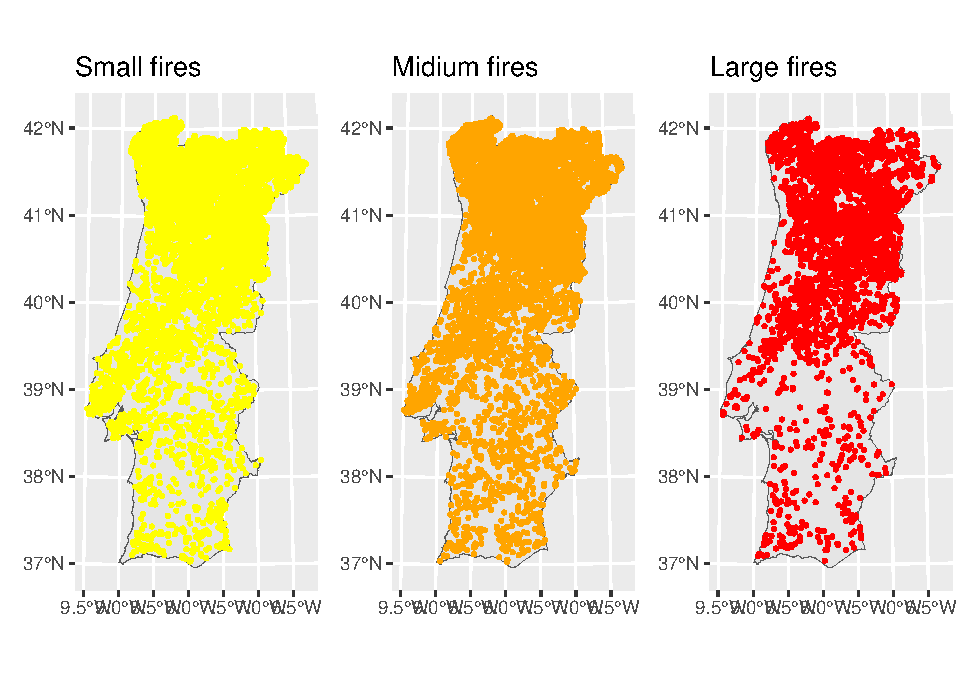
\includegraphics{04-KDE_files/figure-latex/plot-FFsubsets-1} \end{center}

\subsubsection{FF-subsets based on their geographical distribution}\label{ff-subsets-based-on-their-geographical-distribution}

In continental Portugal, the northern half of the country (above the Tagus River) is characterized by the predominance of forest and semi-natural areas, and by the development of the main cities with their sub-urban ares intermingled with wild land, which makes the northern area highly prone to forest fires.

On the other hand, the southern half of the country is dominated by agricultural areas with mixed and broad-leaved forest concentrated near the south-west coast, which makes this area less affected by forest fires.
For this reason we will consider these two areas separately.

\begin{Shaded}
\begin{Highlighting}[]
\CommentTok{\# Plot the map with all the spatia features}
\FunctionTok{ggplot}\NormalTok{ ()}\SpecialCharTok{+}
  \FunctionTok{geom\_sf}\NormalTok{(}\AttributeTok{data=}\NormalTok{Portugal)}\SpecialCharTok{+}
  \FunctionTok{geom\_sf}\NormalTok{(}\AttributeTok{data=}\NormalTok{river, }\AttributeTok{col=}\StringTok{"blue"}\NormalTok{, }\AttributeTok{size=}\DecValTok{2}\NormalTok{) }\SpecialCharTok{+}
  \FunctionTok{geom\_sf}\NormalTok{(}\AttributeTok{data=}\NormalTok{FFN, }\AttributeTok{size=}\FloatTok{0.3}\NormalTok{, }\AttributeTok{col=}\StringTok{"red"}\NormalTok{) }\SpecialCharTok{+}
  \FunctionTok{geom\_sf}\NormalTok{(}\AttributeTok{data=}\NormalTok{FFS, }\AttributeTok{size=}\FloatTok{0.3}\NormalTok{, }\AttributeTok{col=}\StringTok{"orange"}\NormalTok{) }\SpecialCharTok{+}
  \FunctionTok{ggtitle}\NormalTok{(}\StringTok{"Forest foirest in the northern and southern area"}\NormalTok{) }\SpecialCharTok{+}
  \FunctionTok{theme}\NormalTok{(}\AttributeTok{plot.title=}\FunctionTok{element\_text}\NormalTok{(}\AttributeTok{hjust=}\FloatTok{0.5}\NormalTok{)) }\SpecialCharTok{+}
 \FunctionTok{coord\_sf}\NormalTok{()}
\end{Highlighting}
\end{Shaded}

\begin{center}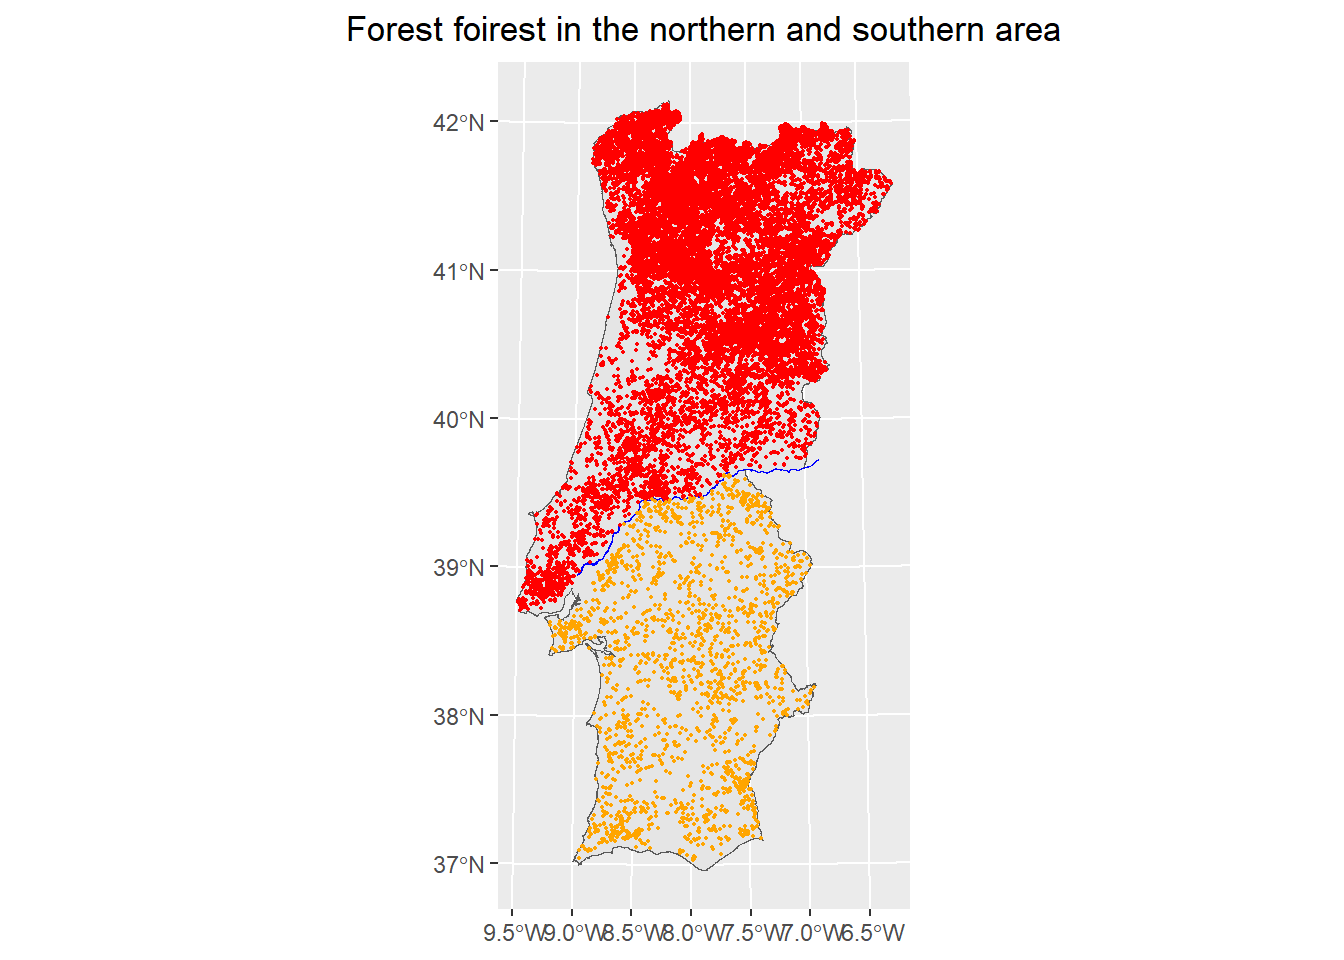
\includegraphics{04-KDE_files/figure-latex/plot-FFN-FFS-1} \end{center}

\subsubsection{Extract time and PTS object}\label{extract-time-and-pts-object}

The function \texttt{stkhat}\textbf{,} included in the library \textbf{spancs} \citep{Rowlingson_2024}, allows to compute the space-time Ripley's K-function.
As you can see from the R Documentation (command: \texttt{help(stkhat)}), same data manipulations are necessary to transform the input data in a compatible data frame format.
Namely the user needs to specify:

\begin{itemize}
\tightlist
\item
  the input forest fires dataset, with the coordinates to geolocalize each event (\texttt{pts})
\item
  a vector of times, defined by the starting date of ignition (\texttt{times})
\item
  a polygon of class matrix enclosing the input dataset (\texttt{poly}\emph{)}
\item
  a vector for the spatial distance (\texttt{s}) and a vector for the temporal length (\texttt{tm})
\end{itemize}

\begin{Shaded}
\begin{Highlighting}[]
\CommentTok{\# Extract "pts" (divided by 1000 to compute in Km)}
\NormalTok{FFN\_pts }\OtherTok{\textless{}{-}} \FunctionTok{as.points}\NormalTok{(FFN}\SpecialCharTok{$}\NormalTok{X}\SpecialCharTok{/}\DecValTok{1000}\NormalTok{, FFN}\SpecialCharTok{$}\NormalTok{Y}\SpecialCharTok{/}\DecValTok{1000}\NormalTok{) }
\NormalTok{FFN\_times}\OtherTok{\textless{}{-}}\NormalTok{FFN}\SpecialCharTok{$}\NormalTok{Year }\CommentTok{\# extract "times"}

\CommentTok{\# Extract the coordinates (in Km):}
\NormalTok{PTN\_xy}\OtherTok{\textless{}{-}}\FunctionTok{st\_coordinates}\NormalTok{(PortN}\SpecialCharTok{$}\NormalTok{geometry}\SpecialCharTok{/}\DecValTok{1000}\NormalTok{) }

\CommentTok{\# Define the matrix with the set of bounding points ("poly") enclosing the input dataset:}
\NormalTok{FFN\_poly}\OtherTok{\textless{}{-}}\NormalTok{PTN\_xy[, }\SpecialCharTok{{-}}\FunctionTok{c}\NormalTok{(}\DecValTok{3}\NormalTok{,}\DecValTok{4}\NormalTok{)] }
\end{Highlighting}
\end{Shaded}

\subsubsection{Compute the ST K-function}\label{compute-the-st-k-function}

We compute the space-time K-function for forest fires in the northern area.
Since the computation can take a long time (about 20 mints), we propose you to load directly the output R object provided (\emph{STK\_North\_10y}).
The general code is also provided, but preceded by the hashtag, so it is not treated as a command: you have to remove \# if you wish to evaluate the code.

\begin{itemize}
\tightlist
\item
  We consider here a subset of forest fires events occurred in the period 2001-2010.
\item
  The parameters \texttt{s} and \texttt{tm} are defined here as follows: \texttt{s}, each kilometer distance up to ten kilometers; \texttt{tm}, each year up to five years.
\end{itemize}

\textbf{NB}: If you wish to run the code, remove \# to make it work

\begin{Shaded}
\begin{Highlighting}[]
\CommentTok{\# Run stkhat function for Northen fires (subset of firs 11 years):}

\CommentTok{\#STK\_North\_10y \textless{}{-} stkhat(pts=FFN\_pts, times=FFN\_times, poly=FFN\_poly, c(2001,2010), seq(0,10,1), seq(0,5,1)) }

\CommentTok{\#str(STK\_North\_10y)}
\end{Highlighting}
\end{Shaded}

\begin{Shaded}
\begin{Highlighting}[]
\CommentTok{\# Open stkhat documentation}
\FunctionTok{help}\NormalTok{(stkhat)}
\end{Highlighting}
\end{Shaded}

\begin{Shaded}
\begin{Highlighting}[]
\FunctionTok{library}\NormalTok{(readr)}

\NormalTok{STK\_North\_10y }\OtherTok{\textless{}{-}} \FunctionTok{readRDS}\NormalTok{(}\StringTok{"data/KDE/STK\_North\_10y.RData"}\NormalTok{)}

\FunctionTok{str}\NormalTok{(STK\_North\_10y)}
\end{Highlighting}
\end{Shaded}

\begin{verbatim}
## List of 5
##  $ s  : num [1:11] 0 1 2 3 4 5 6 7 8 9 ...
##  $ t  : num [1:6] 0 1 2 3 4 5
##  $ ks : num [1:11] 1.61e-04 9.03 2.98e+01 6.18e+01 1.05e+02 ...
##  $ kt : num [1:6] 0.814 2.29 3.596 4.827 6.085 ...
##  $ kst: num [1:11, 1:6] 1.45e-03 1.06e+01 3.75e+01 7.47e+01 1.22e+02 ...
\end{verbatim}

\subsubsection{Assess the ST clustering behavior}\label{assess-the-st-clustering-behavior}

In the following section you will explore and plot the values of the three components produced as outputs of the function \texttt{stkhat}: the spatial K-function (\texttt{ks}), the temporal K-function (\texttt{kt}); the space-time K-function (\texttt{kst}).
Then, you will plot the perspective 3D-plot of \(D(s,t)\) to evaluate the space-time clustering behavior of forest fires in the present case study.
The multifaceted shape of this function, along with the spatial and the temporal dimension, can help to identify peaks of clustering.
The corresponding values can be attributed to the bandwidth of the kernel density estimator allowing to elaborate smoothed density maps in the last step of this lab.

\paragraph{\texorpdfstring{Plot the \texttt{stkhat}'s outputs}{Plot the stkhat's outputs}}\label{plot-the-stkhats-outputs}

\begin{itemize}
\tightlist
\item
  \textbf{Plot of the purely spatial and the purely temporal K function.}
\end{itemize}

\begin{Shaded}
\begin{Highlighting}[]
\CommentTok{\# Plot of the purely spatial K function}
\FunctionTok{plot}\NormalTok{(STK\_North\_10y}\SpecialCharTok{$}\NormalTok{s, STK\_North\_10y}\SpecialCharTok{$}\NormalTok{ks, }\AttributeTok{type=}\StringTok{"l"}\NormalTok{, }\AttributeTok{xlab=}\StringTok{"distance"}\NormalTok{, }\AttributeTok{ylab=}\StringTok{"Estimated Ks"}\NormalTok{, }\AttributeTok{main=}\StringTok{"Spatial K function"}\NormalTok{)}
\FunctionTok{lines}\NormalTok{(STK\_North\_10y}\SpecialCharTok{$}\NormalTok{s, pi}\SpecialCharTok{*}\NormalTok{STK\_North\_10y}\SpecialCharTok{$}\NormalTok{s}\SpecialCharTok{\^{}}\DecValTok{2}\NormalTok{, }\AttributeTok{type=}\StringTok{"l"}\NormalTok{, }\AttributeTok{col=}\StringTok{"red"}\NormalTok{)}
\end{Highlighting}
\end{Shaded}

\begin{center}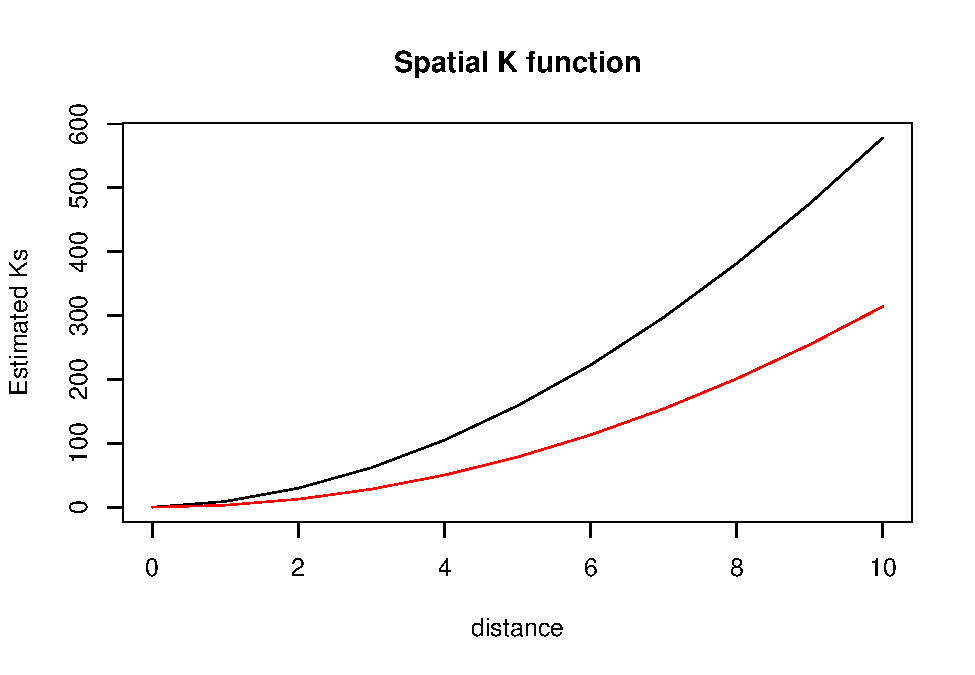
\includegraphics{04-KDE_files/figure-latex/plot-stk-1} \end{center}

\begin{Shaded}
\begin{Highlighting}[]
\CommentTok{\# Plot of the purely temporal K{-}function}
\FunctionTok{plot}\NormalTok{(STK\_North\_10y}\SpecialCharTok{$}\NormalTok{t, STK\_North\_10y}\SpecialCharTok{$}\NormalTok{kt, }\AttributeTok{type=}\StringTok{"l"}\NormalTok{, }\AttributeTok{xlab=}\StringTok{"time"}\NormalTok{, }\AttributeTok{ylab=}\StringTok{"Estimated Kt"}\NormalTok{, }\AttributeTok{main=}\StringTok{"Temporal K function"}\NormalTok{)}
\FunctionTok{lines}\NormalTok{(STK\_North\_10y}\SpecialCharTok{$}\NormalTok{t, }\DecValTok{2}\SpecialCharTok{*}\NormalTok{STK\_North\_10y}\SpecialCharTok{$}\NormalTok{t, }\AttributeTok{type=}\StringTok{"l"}\NormalTok{, }\AttributeTok{col=}\StringTok{"red"}\NormalTok{)}
\end{Highlighting}
\end{Shaded}

\begin{center}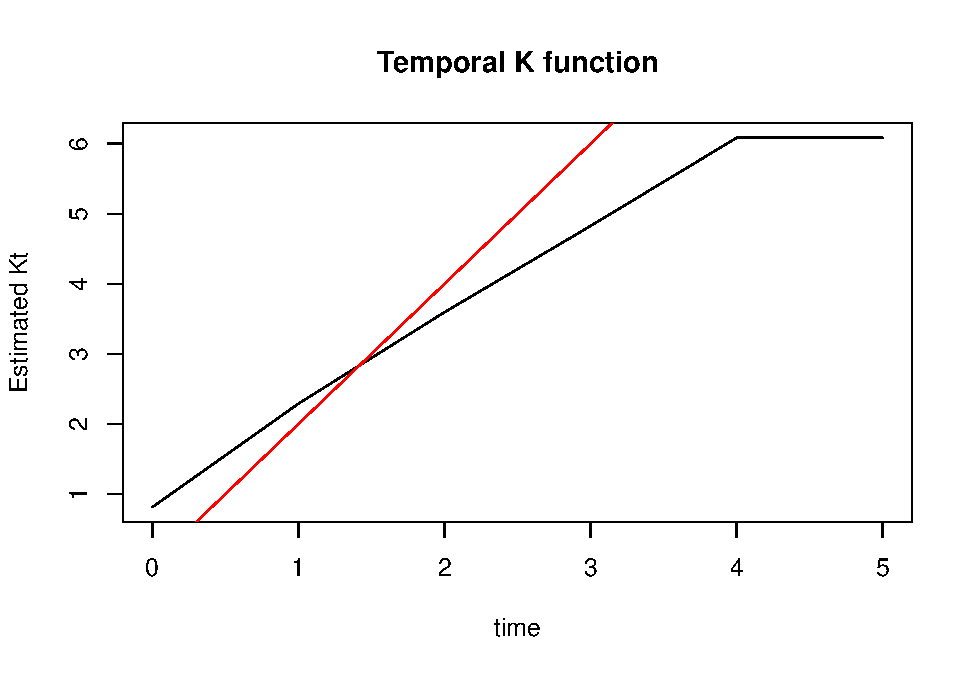
\includegraphics{04-KDE_files/figure-latex/plot-stk-2} \end{center}

\begin{itemize}
\tightlist
\item
  \textbf{Plot the space-time D-plot}
\end{itemize}

\begin{Shaded}
\begin{Highlighting}[]
\CommentTok{\# Define the function: D(s,t)=K(s,t){-}[K(s)*K(t)]}

\NormalTok{Dplot }\OtherTok{\textless{}{-}} \ControlFlowTok{function}\NormalTok{ (stkhat, }\AttributeTok{Dzero =} \ConstantTok{FALSE}\NormalTok{, }\AttributeTok{main=}\ConstantTok{TRUE}\NormalTok{)  \{}

\NormalTok{  oprod }\OtherTok{\textless{}{-}} \FunctionTok{outer}\NormalTok{(stkhat}\SpecialCharTok{$}\NormalTok{ks, stkhat}\SpecialCharTok{$}\NormalTok{kt)}
\NormalTok{    st.D }\OtherTok{\textless{}{-}}\NormalTok{ stkhat}\SpecialCharTok{$}\NormalTok{kst }\SpecialCharTok{{-}}\NormalTok{ oprod}
        \FunctionTok{persp}\NormalTok{(stkhat}\SpecialCharTok{$}\NormalTok{s, stkhat}\SpecialCharTok{$}\NormalTok{t, st.D, }\AttributeTok{xlab =} \StringTok{"Distance (Km)"}\NormalTok{, }\AttributeTok{ylab =} \StringTok{"Time (years)"}\NormalTok{,}
            \AttributeTok{zlab =} \StringTok{"D(s,t)"}\NormalTok{, }\AttributeTok{expand =} \FloatTok{0.5}\NormalTok{, }\AttributeTok{ticktype =} \StringTok{"detailed"}\NormalTok{,}
            \AttributeTok{theta =} \SpecialCharTok{{-}}\DecValTok{45}\NormalTok{, }\AttributeTok{shade =} \FloatTok{0.75}\NormalTok{, }\AttributeTok{cex =} \FloatTok{0.7}\NormalTok{, }\AttributeTok{ltheta=}\DecValTok{120}\NormalTok{, }\AttributeTok{col=}\StringTok{"cyan1"}\NormalTok{, }\AttributeTok{font.lab=}\DecValTok{2}\NormalTok{)}
\NormalTok{           \}}

\FunctionTok{Dplot}\NormalTok{(STK\_North\_10y)}
\FunctionTok{title}\NormalTok{(}\StringTok{"Dplot Nothern Fires"}\NormalTok{)}
\end{Highlighting}
\end{Shaded}

\begin{center}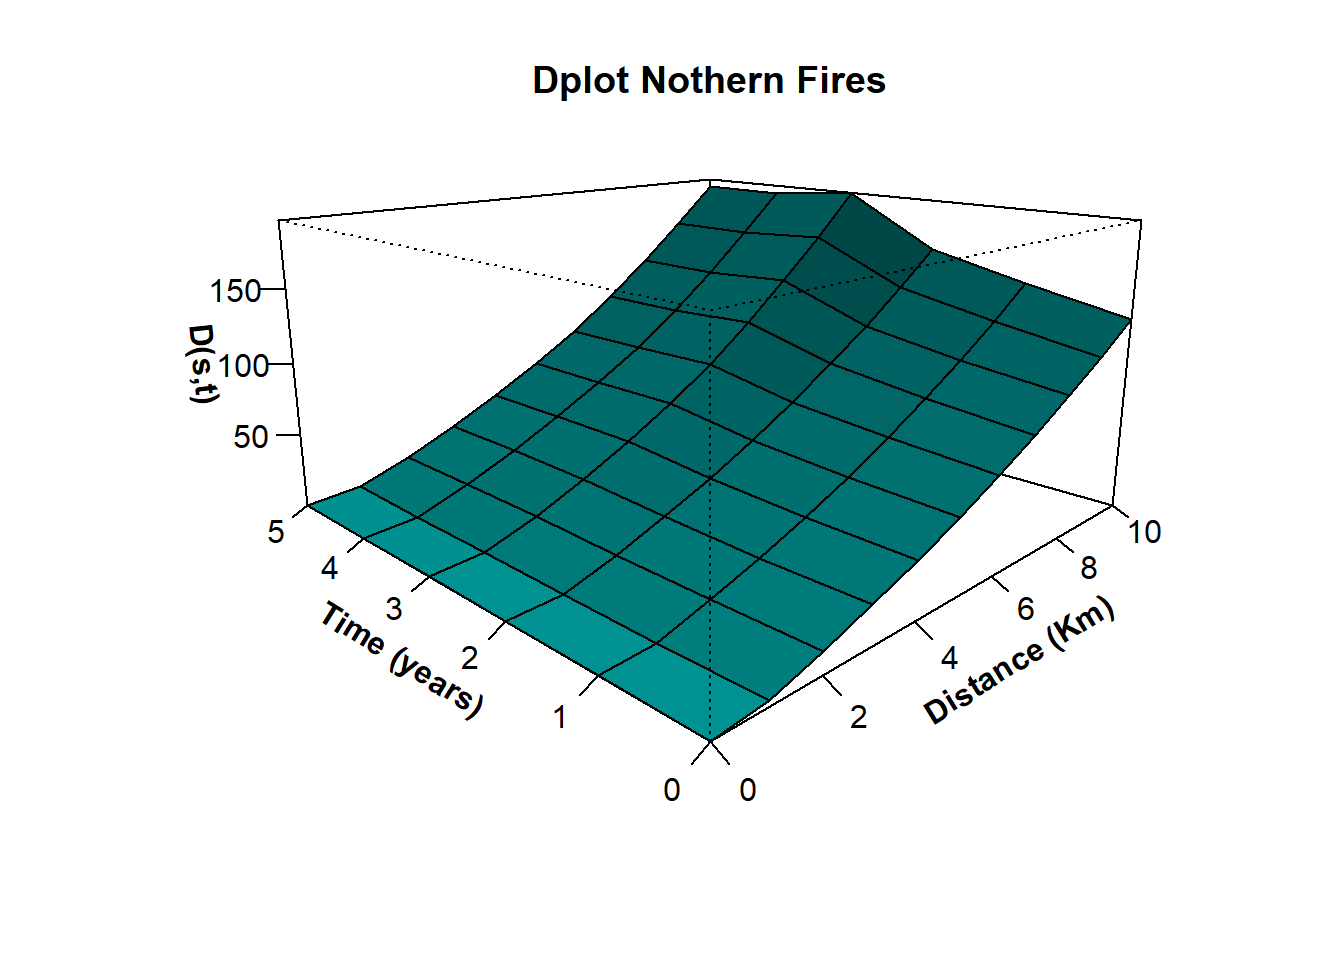
\includegraphics{04-KDE_files/figure-latex/D-plot-1} \end{center}

\subsubsection{Compute the ST Kernel Density Estimator}\label{compute-the-st-kernel-density-estimator}

The multifaceted shape the D-Plot identify peaks of clustering at a time interval of 3 year.
In space, events are clustered at every distance, so in this case we use the maximum distance-value (10 km).
These two values are attributed to the bandwidth of the space-time KDE allowing to elaborate smoothed density maps.
To this end, we use the function \texttt{kernel3d}\textbf{,} included in the library \textbf{spancs} \citep{Rowlingson_2024} too.

\begin{Shaded}
\begin{Highlighting}[]
\CommentTok{\# Open the help to analyse the parameter of this function: }
\FunctionTok{help}\NormalTok{(kernel3d)}
\end{Highlighting}
\end{Shaded}

\begin{Shaded}
\begin{Highlighting}[]
\CommentTok{\# Compute the spatio{-}temporal KDE }
\NormalTok{KDE\_FFN}\OtherTok{\textless{}{-}}\FunctionTok{kernel3d}\NormalTok{(FFN\_pts, FFN\_times, }\FunctionTok{seq}\NormalTok{(}\DecValTok{80}\NormalTok{, }\DecValTok{362}\NormalTok{, }\DecValTok{1}\NormalTok{), }\FunctionTok{seq}\NormalTok{(}\DecValTok{180}\NormalTok{, }\DecValTok{580}\NormalTok{, }\DecValTok{1}\NormalTok{), }\FunctionTok{seq}\NormalTok{(}\DecValTok{1990}\NormalTok{,}\DecValTok{2013}\NormalTok{,}\DecValTok{1}\NormalTok{), }\DecValTok{10}\NormalTok{, }\DecValTok{3}\NormalTok{)}

\CommentTok{\#Inspect the results}
\FunctionTok{summary}\NormalTok{(KDE\_FFN}\SpecialCharTok{$}\NormalTok{v)}
\end{Highlighting}
\end{Shaded}

\begin{verbatim}
##      Min.   1st Qu.    Median      Mean   3rd Qu.      Max. 
## 0.0000000 0.0000000 0.0002195 0.0995232 0.1093261 2.1627084
\end{verbatim}

\begin{Shaded}
\begin{Highlighting}[]
\FunctionTok{hist}\NormalTok{(}\FunctionTok{log10}\NormalTok{(KDE\_FFN}\SpecialCharTok{$}\NormalTok{v))}
\end{Highlighting}
\end{Shaded}

\begin{center}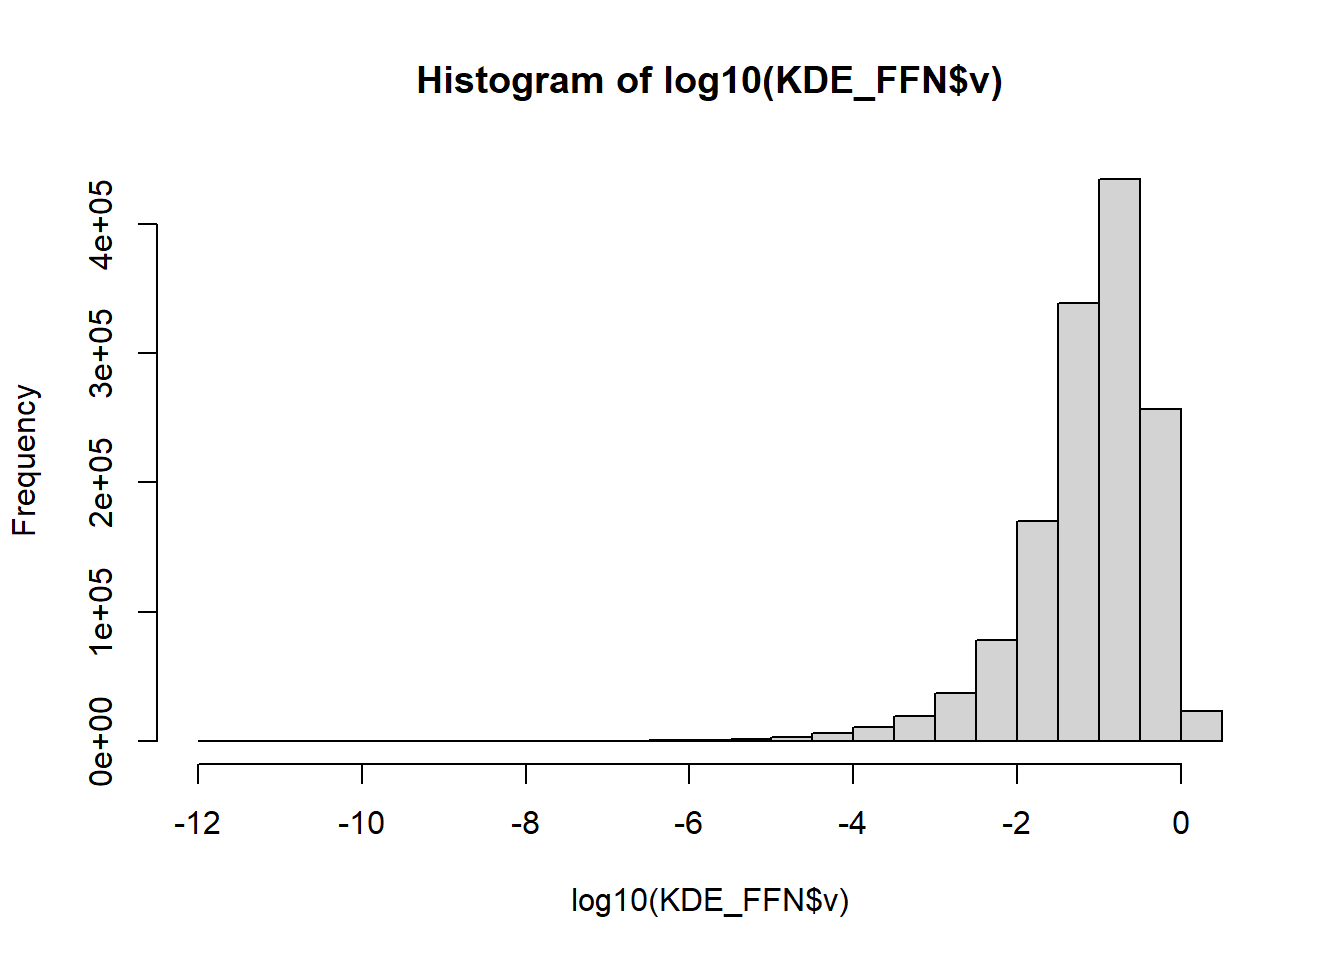
\includegraphics{04-KDE_files/figure-latex/ST-KDE-1} \end{center}

\begin{Shaded}
\begin{Highlighting}[]
\FunctionTok{min}\NormalTok{(KDE\_FFN}\SpecialCharTok{$}\NormalTok{v[KDE\_FFN}\SpecialCharTok{$}\NormalTok{v}\SpecialCharTok{\textgreater{}}\DecValTok{0}\NormalTok{]) }\CommentTok{\#check the lower non{-}zero value }
\end{Highlighting}
\end{Shaded}

\begin{verbatim}
## [1] 2.893333e-12
\end{verbatim}

\begin{Shaded}
\begin{Highlighting}[]
\CommentTok{\# Create quantile clssification }
\NormalTok{Q}\OtherTok{\textless{}{-}}\FunctionTok{quantile}\NormalTok{(KDE\_FFN}\SpecialCharTok{$}\NormalTok{v, }\FunctionTok{seq}\NormalTok{(}\FloatTok{0.5}\NormalTok{,}\DecValTok{1}\NormalTok{,}\FloatTok{0.05}\NormalTok{))}
\NormalTok{Q}
\end{Highlighting}
\end{Shaded}

\begin{verbatim}
##          50%          55%          60%          65%          70%          75% 
## 0.0002194741 0.0097073381 0.0263666531 0.0478856382 0.0748979448 0.1093260662 
##          80%          85%          90%          95%         100% 
## 0.1560709189 0.2210177893 0.3232627322 0.5162620818 2.1627084390
\end{verbatim}

\begin{Shaded}
\begin{Highlighting}[]
\CommentTok{\# Create a blue/red palette}
\NormalTok{pal}\OtherTok{\textless{}{-}}\FunctionTok{colorRampPalette}\NormalTok{(}\FunctionTok{c}\NormalTok{(}\StringTok{"grey"}\NormalTok{,}\StringTok{"blue"}\NormalTok{,}\StringTok{"green"}\NormalTok{, }\StringTok{"yellow"}\NormalTok{,}\StringTok{"orange"}\NormalTok{, }\StringTok{"red"}\NormalTok{ ))}
\NormalTok{colsR}\OtherTok{\textless{}{-}}\FunctionTok{pal}\NormalTok{(}\FunctionTok{length}\NormalTok{(Q)}\SpecialCharTok{{-}}\DecValTok{1}\NormalTok{)}

\CommentTok{\# Display classes}
\FunctionTok{pie}\NormalTok{(Q, }\AttributeTok{clockwise=}\ConstantTok{TRUE}\NormalTok{, }\AttributeTok{labels=}\FunctionTok{round}\NormalTok{(Q, }\AttributeTok{digits=}\DecValTok{2}\NormalTok{), }\AttributeTok{border=}\StringTok{"white"}\NormalTok{, }\AttributeTok{col=}\NormalTok{colsR)}
\end{Highlighting}
\end{Shaded}

\begin{center}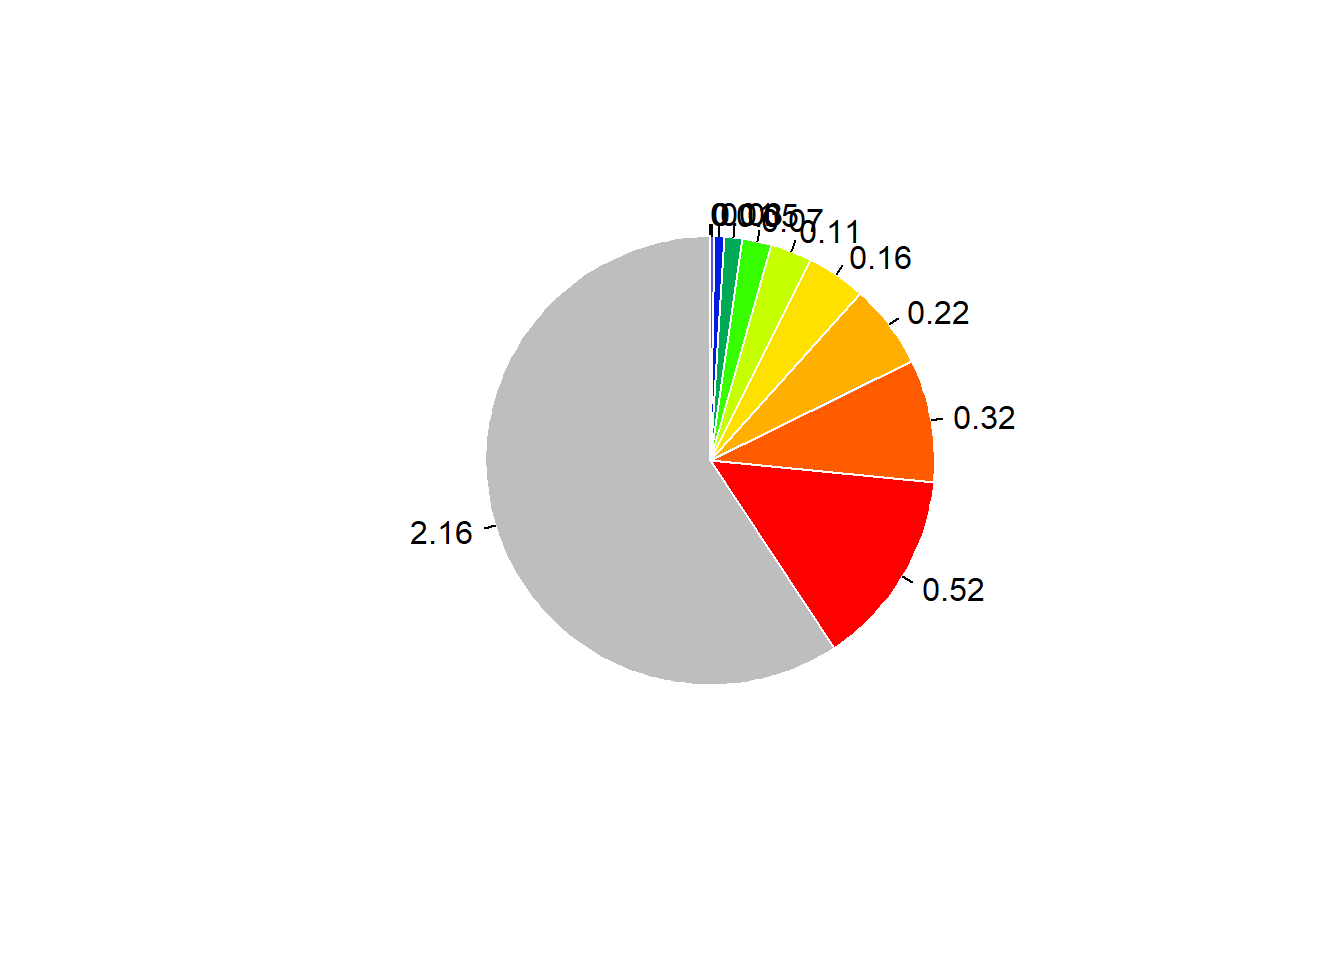
\includegraphics{04-KDE_files/figure-latex/plot-KDE-1} \end{center}

\begin{Shaded}
\begin{Highlighting}[]
\CommentTok{\# Plot KDE maps for selected years}
\NormalTok{oldpar}\OtherTok{\textless{}{-}}\FunctionTok{par}\NormalTok{(}\AttributeTok{mfrow=}\FunctionTok{c}\NormalTok{(}\DecValTok{5}\NormalTok{,}\DecValTok{5}\NormalTok{), }\AttributeTok{mar=}\FunctionTok{c}\NormalTok{(}\DecValTok{1}\NormalTok{,}\DecValTok{1}\NormalTok{,}\DecValTok{1}\NormalTok{,}\DecValTok{1}\NormalTok{))}
\ControlFlowTok{for}\NormalTok{ (i }\ControlFlowTok{in} \DecValTok{1}\SpecialCharTok{:}\DecValTok{24}\NormalTok{)\{}
\NormalTok{ (}\FunctionTok{image}\NormalTok{(}\FunctionTok{seq}\NormalTok{(}\DecValTok{80}\NormalTok{, }\DecValTok{362}\NormalTok{, }\DecValTok{1}\NormalTok{), }\FunctionTok{seq}\NormalTok{(}\DecValTok{180}\NormalTok{, }\DecValTok{580}\NormalTok{, }\DecValTok{1}\NormalTok{), KDE\_FFN}\SpecialCharTok{$}\NormalTok{v[,,i], }\AttributeTok{asp=}\DecValTok{1}\NormalTok{, }\AttributeTok{xlab=}\StringTok{""}\NormalTok{, }\AttributeTok{ylab=}\StringTok{""}\NormalTok{, }\AttributeTok{main=}\DecValTok{1989}\SpecialCharTok{+}\NormalTok{i, }\AttributeTok{breaks=}\NormalTok{Q, }\AttributeTok{col=}\NormalTok{colsR))}
\NormalTok{\}}
\end{Highlighting}
\end{Shaded}

\begin{center}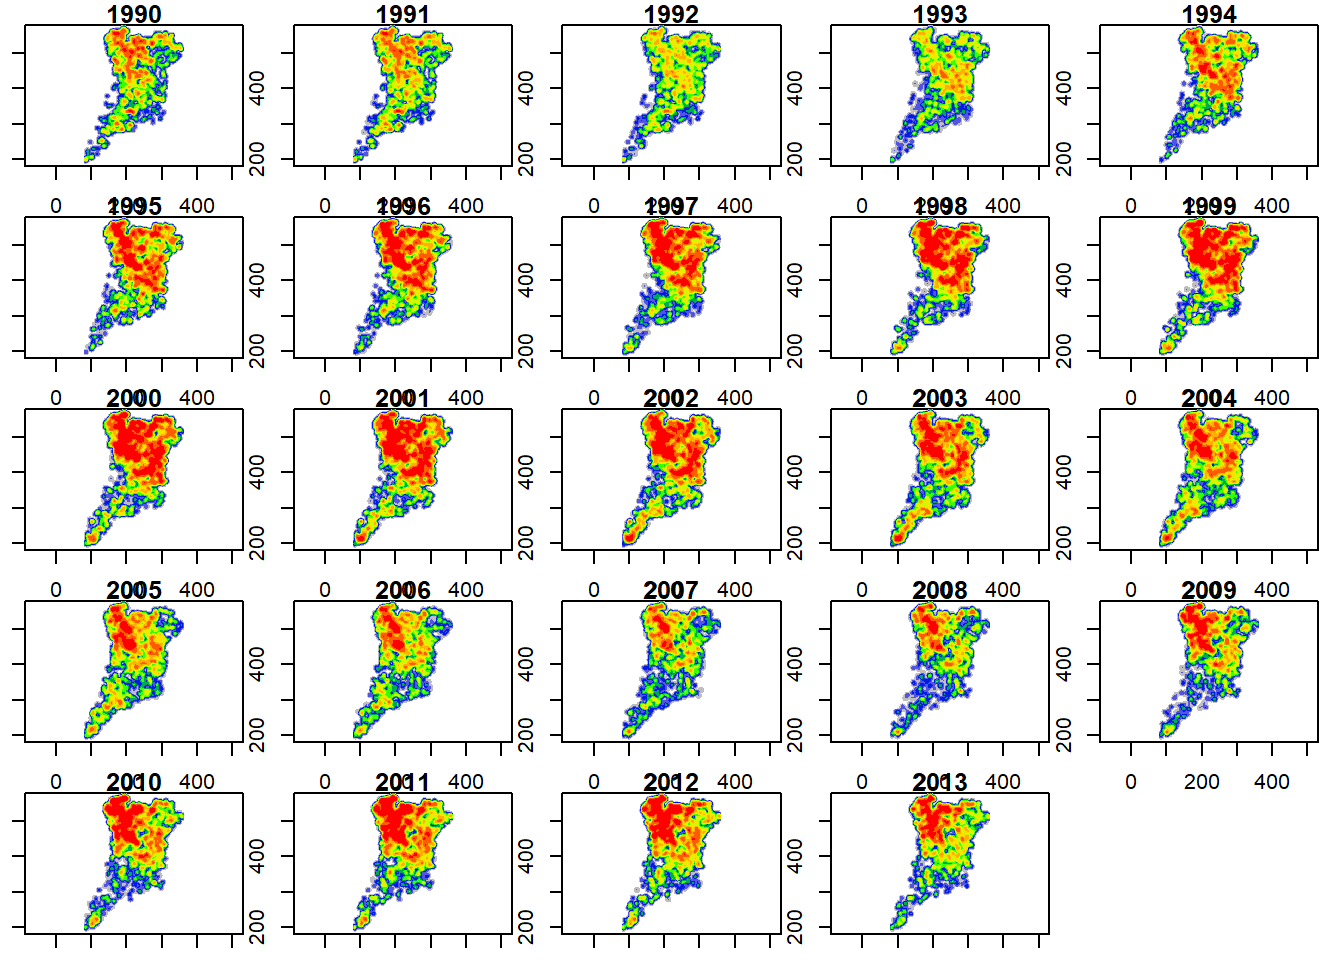
\includegraphics{04-KDE_files/figure-latex/plot-KDE-2} \end{center}

\subsection{Conclusions and further analyses}\label{conclusions-and-further-analyses-1}

This practical computing lab allowed you to asses the global cluster behavior of hazardous events, achieved by using the Ripley's k-function.
In addition, we learned how smoothed density maps can be elaborated from punctual events, namely using the kernel density estimator.
Both the spatial and the temporal dimension have been considered in this case.
As practical case study, you could explore the density distribution of forest fires events through Continental Portugal in the period 1990-2013.
In the northern half of the country, hot spots are present almost on each investigated years, with a higher concentration in the northern areas.

To ensure that everything is perfectly clear, we propose you to do this lab again, by using this time another subset chosen among the available ones including forest fires in the southern area, the small, medium, or the large forest fires dataset.
For whatever dataset you are going to use, try to answer to the following questions.
The reading of the paper \citep{tonini_evolution_2017}, which inspired this lab, can help you in in this task.

\begin{enumerate}
\def\labelenumi{\arabic{enumi}.}
\item
  At which spatial and temporal distance you can observe a peak of clustering?
\item
  By visually inspecting the KDE maps, describe the spatio-temporal density distribution of forest fires events through the study area.
\end{enumerate}

\section{Predictive Mapping of Natural Hazards Using Random Forest}\label{global-rf}

Random Forest (RF) is a robust and widely-used machine learning algorithm particularly suited for predictive mapping in the context of natural hazards and susceptibility assessments.
It operates by constructing multiple decision trees during training, and then aggregating their predictions to improve accuracy and generalizability \citep{breiman_random_2001}.
For the sake of clarity, we define \emph{susceptibility} of an area the potential to experience a particular hazard in the future, based only on the intrinsic local properties of the territory, assessed in terms of relative spatial likelihood.
Machine Learning (ML) based approaches lend themselves particularly well to this purpose.
Essentially ML includes algorithms capable of learning from and making predictions on data by modelling the hidden/non-linear relationships between a set of input variables -- also known as predictors -- and output observations.

In natural hazard and susceptibility mapping, RF can analyze complex relationships between environmental variables such as topography, soil type, vegetation cover, and climate data to predict the likelihood of hazardous events -- like landslides, floods, or earthquakes -- across a landscape.
Its ability to handle large datasets, manage variables interactions, and provide importance rankings for predictor variables, makes it an invaluable tool for generating reliable susceptibility maps, which are crucial for disaster risk management and land-use planning.

\subsection{RF for landslides susceptibility mapping}\label{rf-for-landslides-susceptibility-mapping}

In this application, we explore the capabilities RF to elaborate landslides susceptibility mapping in Canton Vaud, Switzerland.
Landslides are one of the major hazard occurring around the world.
In Switzerland, landslides cause damages to infrastructures and sometimes threaten human lives, especially shallow landslides.
Such slope movements are mainly triggered by intense rainfalls and generally very rapid and hardly predictable.

The research framework that inspired this computing lab refers to a pioneering study in susceptibility mapping for wildfire events by \citep{tonini_machine_2020} and further developed for the assessment of variable importance by \citep{trucchia_machine-learning_2022}.
Analyses have been adapted to the case study of landslides.
The overall methodology is described in the following graphic.

\begin{figure}

{\centering 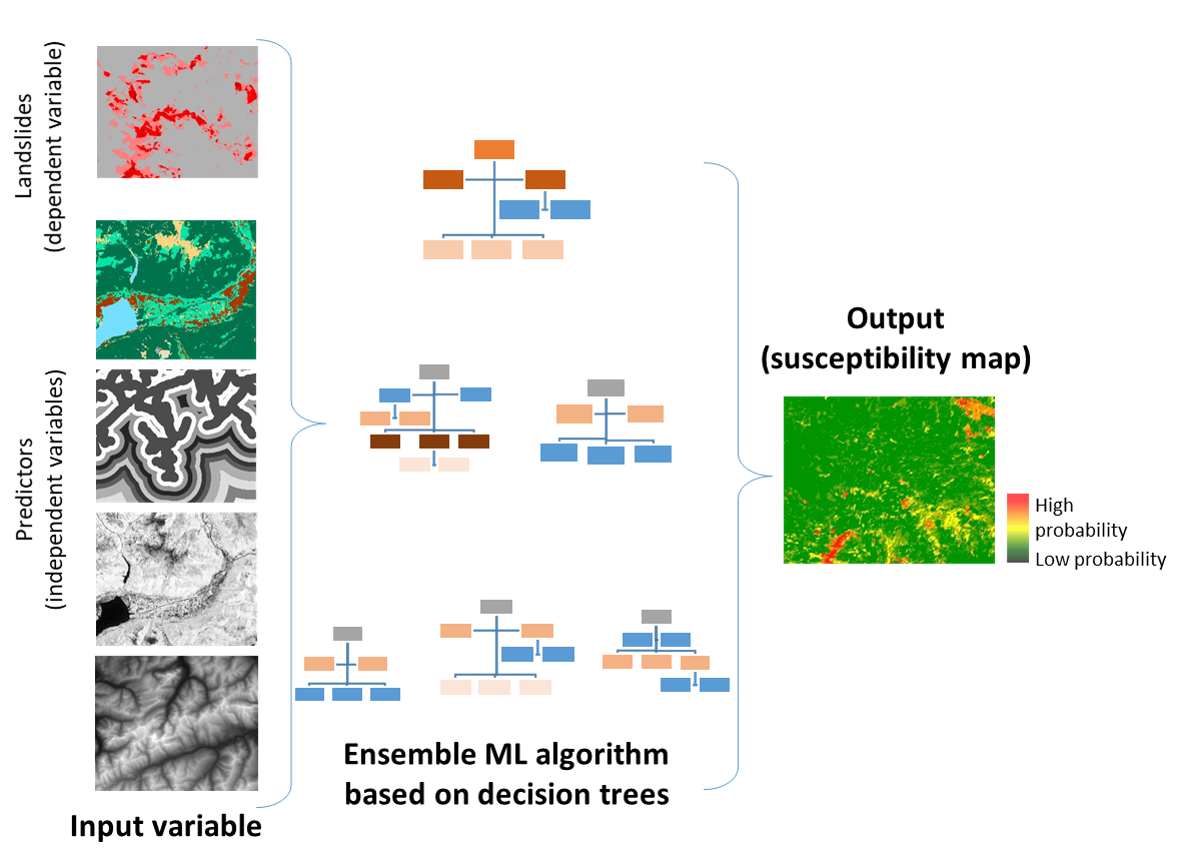
\includegraphics[width=0.8\linewidth,height=0.8\textheight]{images/Methodology} 

}

\caption{Basic elements of the generic methodology \label{Methodology}}\label{fig:gen-met}
\end{figure}

\subsection{Computing lab: Random Forest}\label{computing-lab-random-forest}

\subsubsection{Load the libraries}\label{load-the-libraries-2}

To perform the analysis, you have first to install the following libraries:

\begin{itemize}
\tightlist
\item
  \emph{terra}: methods for spatial data analysis with vector (points, lines, polygons) and raster (grid) data
\item
  \emph{readr}: to provide a fast and friendly way to read tabulat data (like *.csv)
\item
  \emph{randomForest}: classification and regression, based on a forest of trees using random inputs
\item
  \emph{dplyr}: focused on tools for working with data frames
\item
  \emph{pROC}: allowing to compute, analyze ROC curves, and

  \begin{itemize}
  \tightlist
  \item
    \emph{plotROC}\textbf{:} to display ROC curve
  \end{itemize}
\item
  \emph{ggplot2}: a system for declaratively creating graphics
\end{itemize}

\begin{Shaded}
\begin{Highlighting}[]
\FunctionTok{library}\NormalTok{(terra)}
\FunctionTok{library}\NormalTok{(readr) }
\FunctionTok{library}\NormalTok{(randomForest) }
\FunctionTok{library}\NormalTok{(dplyr) }
\FunctionTok{library}\NormalTok{(pROC) }
\FunctionTok{library}\NormalTok{(plotROC) }
\FunctionTok{library}\NormalTok{(ggplot2) }

\NormalTok{(}\FunctionTok{.packages}\NormalTok{())}
\end{Highlighting}
\end{Shaded}

\subsubsection{Load the input datasets}\label{load-the-input-datasets}

In the following you will import the landslides punctual dataset including presences and absences (\emph{LS\_pa}) and the predictor variables (in raster format).
This will enable to perform the exploratory data analyses step and the understanding of the input data structure.

\paragraph{Landslides dataset}\label{landslides-dataset}

The landslide inventory has been provided by the environmental office of the Canton Vaud.
Only shallow landslides are used for susceptibility modelling.
One pixel per landslide-area (namely the one located at the highest elevation) has been extracted.
Since the landslide scarp is located in the upper part of the polygon, it makes sense to consider the highest pixel to characterize each single event.

Our model includes the implementation of the landslide \textbf{pseudo-absences}, which are the areas where the hazardous events did not took place (i.e.~landslide location is known and the mapped footprint areas are available, but the non-landslide areas have to be defined).
Indeed, to assure a good generalization of the model and to avoid the overestimation of the absences, pseudo-absences need to be generated in all the cases where they are not explicitly expressed.
In this case study, an equal number of point as for presences has been randomly generated in the study area, except within landslides polygons, lakes and glaciers (that is what is called ``\emph{validity domain}'', where events could potentially occur).

\begin{Shaded}
\begin{Highlighting}[]
\CommentTok{\# Import the boundary of Canton Vaud }
\NormalTok{Vaud }\OtherTok{\textless{}{-}} \FunctionTok{vect}\NormalTok{(}\StringTok{"data/RF/Vaud\_CH.shp"}\NormalTok{)}
\NormalTok{Lake }\OtherTok{\textless{}{-}} \FunctionTok{vect}\NormalTok{(}\StringTok{"data/RF/Lakes\_VD.shp"}\NormalTok{)}


\CommentTok{\# Import the landslides dataset (dependent variable)}
\NormalTok{LS\_pa }\OtherTok{\textless{}{-}} \FunctionTok{read.csv}\NormalTok{(}\StringTok{"data/RF/LS\_pa.csv"}\NormalTok{) }

\CommentTok{\# Convert the numeric values (0/1) as factor }
\DocumentationTok{\#\#(i.e. categorical value)}
\NormalTok{LS\_pa}\SpecialCharTok{$}\NormalTok{LS}\OtherTok{\textless{}{-}}\FunctionTok{as.factor}\NormalTok{(LS\_pa}\SpecialCharTok{$}\NormalTok{LS)}

\NormalTok{LS\_vect}\OtherTok{\textless{}{-}}\FunctionTok{vect}\NormalTok{(LS\_pa, }\AttributeTok{geom=}\FunctionTok{c}\NormalTok{(}\StringTok{"X"}\NormalTok{, }\StringTok{"Y"}\NormalTok{),}\AttributeTok{crs=}\FunctionTok{crs}\NormalTok{(Vaud))}

\CommentTok{\# Display the structure (str) and result summaries (summary)}
\FunctionTok{str}\NormalTok{(LS\_vect)}
\end{Highlighting}
\end{Shaded}

\begin{verbatim}
## S4 class 'SpatVector' [package "terra"]
\end{verbatim}

\begin{Shaded}
\begin{Highlighting}[]
\FunctionTok{summary}\NormalTok{(LS\_vect)}
\end{Highlighting}
\end{Shaded}

\begin{verbatim}
##  LS      
##  0:2594  
##  1:2594
\end{verbatim}

\begin{Shaded}
\begin{Highlighting}[]
\CommentTok{\# Plot the events}
\FunctionTok{plot}\NormalTok{(Vaud)}
\FunctionTok{plot}\NormalTok{(Lake, }\AttributeTok{col=}\StringTok{"lightblue"}\NormalTok{, }\AttributeTok{add=}\ConstantTok{TRUE}\NormalTok{)}
\FunctionTok{plot}\NormalTok{(LS\_vect, }\AttributeTok{col=}\NormalTok{LS\_pa}\SpecialCharTok{$}\NormalTok{LS, }\AttributeTok{pch=}\DecValTok{20}\NormalTok{, }\AttributeTok{cex=}\FloatTok{0.5}\NormalTok{, }\AttributeTok{add=}\ConstantTok{TRUE}\NormalTok{)}
\end{Highlighting}
\end{Shaded}

\begin{center}\includegraphics{05-RF_Cl_files/figure-latex/import-data-1} \end{center}

\paragraph{Predictor variables}\label{predictor-variables}

Selecting predictive variables is a key stage in landslide susceptibility modelling when using a data-driven approach.
There is no consensus about the number of variables and which variables should be used.
In the present exercise we will use the following:

\begin{itemize}
\item
  \textbf{DEM (digital elevation model)}: provided by the Swiss Federal Office of Topography.
  The elevation is not a direct conditioning factor for landslide; however, it can reflect differences in vegetation characteristics and soil.
\item
  \textbf{Slope}: is one of the most explicating factor in landslide susceptibility modelling.
\end{itemize}

\[Slope = arctan(\sqrt{(dz/dx)^2 + (dz/dy)^2)} * (\pi/2)\]

\begin{itemize}
\item
  \textbf{Curvature}: curvature is widely used in landslide susceptibility modelling.
  It allows assessing the water flow acceleration and sediment transport process (\emph{profile curvature}) and the water flow propensity to converge and diverge (\emph{plan curvature}).
  They have been derived from DEM and directly provided here.
\item
  \textbf{TWI (topographical water index)}: topography plays a key role in the spatial distribution of soil hydrological conditions.
  Defining \(\alpha\) as the upslope contributing area describing the propensity of a cell to receive water, and \(\beta\) as the slope angle, TWI (compute by the formula below), reflects the propensity of a cell to evacuate water:
\end{itemize}

\[TWI=ln(\alpha/tan(\beta))\]

\begin{itemize}
\item
  \textbf{Distance to roads}: roads build in mountainous areas often cut the slope, weakening the cohesion of the soil.
  Moreover, roads surfaces are highly impermeable.
  This raster has been elaborated by computing the euclidean distance from the swissTLMRegio map where roads are represented by lines.
\item
  \textbf{Land Cover}: developed by the Swiss administration and based on aerial photographs and control points.
  It includes 27 categories distributed in the following 6 domains: human modified surfaces, herbaceous vegetation, shrubs vegetation, tree vegetation, surfaces without vegetation, water surfaces (glaciers included).
\item
  \textbf{Geology}: the use of the lithology increase the performance of the susceptibility landslide models.
  We use here the map elaborated by the Canton Vaud, defining the geotypes and reclassified in 10 classes in order to differentiate sedimentary rocks.
\end{itemize}

Than the predictor variables have to be aggregated into a single object, storing multiple rasters.
We use here the generic function \texttt{c} to combine the single raster into a multiple-raster object.

\begin{Shaded}
\begin{Highlighting}[]
\DocumentationTok{\#\# Import raster (independent variables) 25 meter resolution}

\NormalTok{landCover}\OtherTok{\textless{}{-}}\FunctionTok{as.factor}\NormalTok{(}\FunctionTok{rast}\NormalTok{(}\StringTok{"data/RF/landCover.tif"}\NormalTok{))}
\NormalTok{geology}\OtherTok{\textless{}{-}}\FunctionTok{as.factor}\NormalTok{(}\FunctionTok{rast}\NormalTok{(}\StringTok{"data/RF/geology.tif"}\NormalTok{))}

\NormalTok{planCurv}\OtherTok{\textless{}{-}}\FunctionTok{rast}\NormalTok{(}\StringTok{"data/RF/plan\_curvature.tif"}\NormalTok{)}\SpecialCharTok{/}\DecValTok{100}
\NormalTok{profCurv}\OtherTok{\textless{}{-}}\FunctionTok{rast}\NormalTok{(}\StringTok{"data/RF/profil\_curvature.tif"}\NormalTok{)}\SpecialCharTok{/}\DecValTok{100} 
\CommentTok{\# this because the input values was originally multiplied by 100}

\NormalTok{TWI }\OtherTok{\textless{}{-}} \FunctionTok{rast}\NormalTok{(}\StringTok{"data/RF/TWI.tif"}\NormalTok{)}
\NormalTok{Slope }\OtherTok{\textless{}{-}} \FunctionTok{rast}\NormalTok{(}\StringTok{"data/RF/Slope.tif"}\NormalTok{)}
\NormalTok{dem }\OtherTok{\textless{}{-}} \FunctionTok{rast}\NormalTok{(}\StringTok{"data/RF/DEM.tif"}\NormalTok{)}
\NormalTok{dist }\OtherTok{\textless{}{-}} \FunctionTok{rast}\NormalTok{(}\StringTok{"data/RF/dist\_roads.tif"}\NormalTok{)}

\CommentTok{\# Combine raster}

\NormalTok{features}\OtherTok{\textless{}{-}}\FunctionTok{c}\NormalTok{(dist, dem, landCover, TWI, planCurv, profCurv, Slope, geology)}

\CommentTok{\# Renames the input features }
\FunctionTok{names}\NormalTok{(features)}\OtherTok{\textless{}{-}}\FunctionTok{c}\NormalTok{(}\StringTok{"distRoad"}\NormalTok{, }\StringTok{"DEM"}\NormalTok{, }\StringTok{"landCover"}\NormalTok{, }\StringTok{"TWI"}\NormalTok{, }\StringTok{"planCurv"}\NormalTok{, }\StringTok{"profCurv"}\NormalTok{, }\StringTok{"slope"}\NormalTok{, }\StringTok{"geology"}\NormalTok{)}

\CommentTok{\# Mask to DEM extension}
\NormalTok{features }\OtherTok{\textless{}{-}}\NormalTok{ terra}\SpecialCharTok{::}\FunctionTok{mask}\NormalTok{(features, dem)}

\FunctionTok{plot}\NormalTok{(features)}
\end{Highlighting}
\end{Shaded}

\begin{center}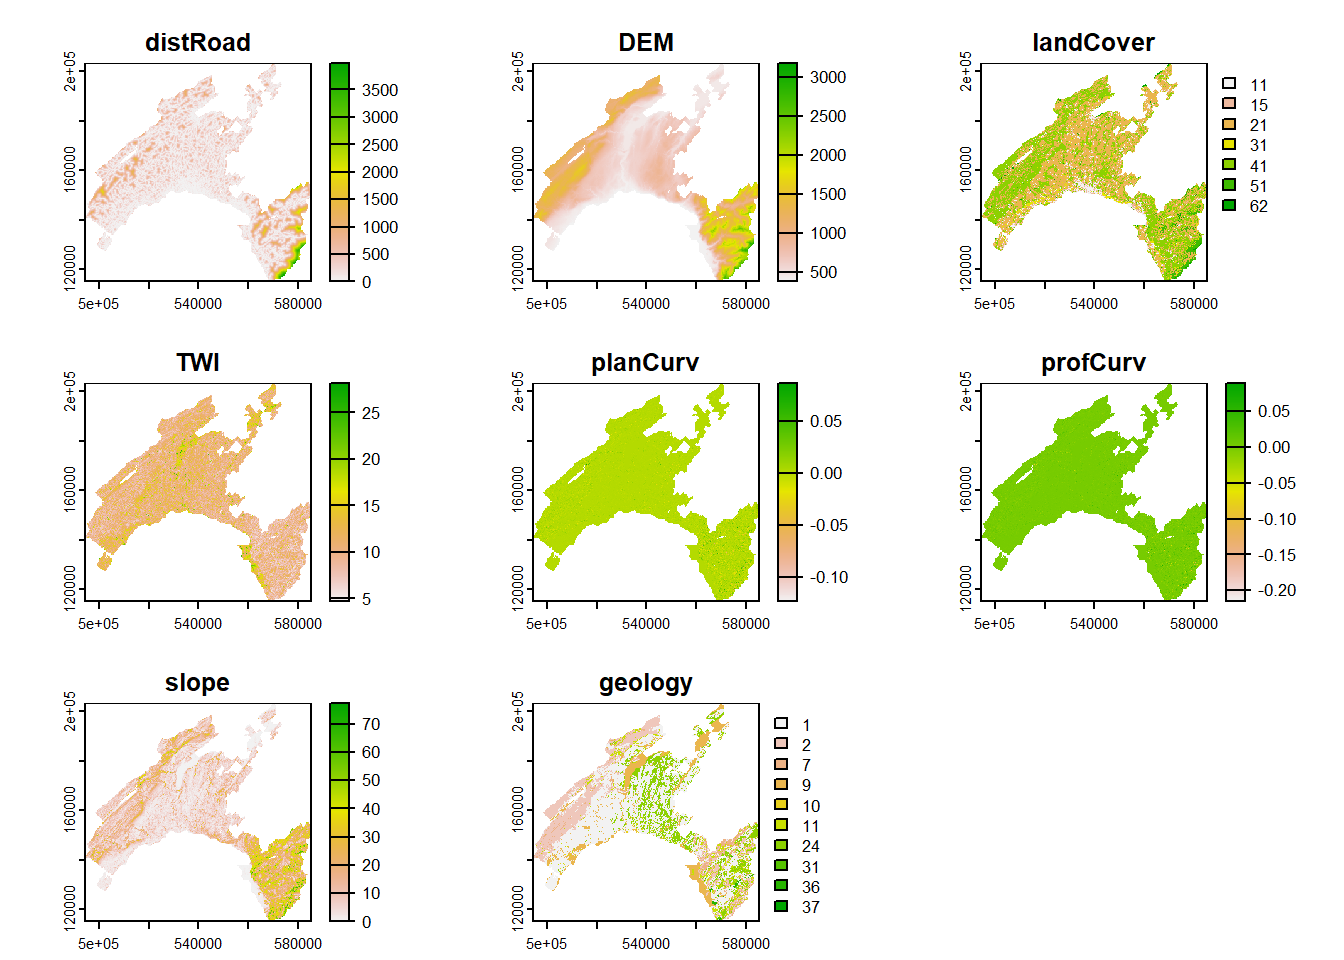
\includegraphics{05-RF_Cl_files/figure-latex/import-raster-1} \end{center}

\subsubsection{The use of categorical variables in Machine Learning}\label{the-use-of-categorical-variables-in-machine-learning}

The majority of ML algorithms (e.g., support vector machines, artificial neural network, deep learning) makes predictions on the base of the proximity between the values of the predictors, computed in terms of euclidean distance.
This means that these algorithms can not handle directly categorical values (i.e., qualitative descriptors).
Thus, in most of the cases, categorical variables need to be transformed into a numerical format.
One of the advantage of using Random Forest (as implemented in R) is that it can handle directly categorical variables, since the algorithm operate by constructing a multitude of decision trees at training time and the best split is chosen just by counting the proportion of each class observation.

To understand the characteristics of the categorical variables, you can plot the tow raster \textbf{Land Cover} and \textbf{Geology} by using their original classes and look at the attribute table to analyse the corresponding definitions.

\begin{Shaded}
\begin{Highlighting}[]
\FunctionTok{plot}\NormalTok{(geology)}
\end{Highlighting}
\end{Shaded}

\begin{center}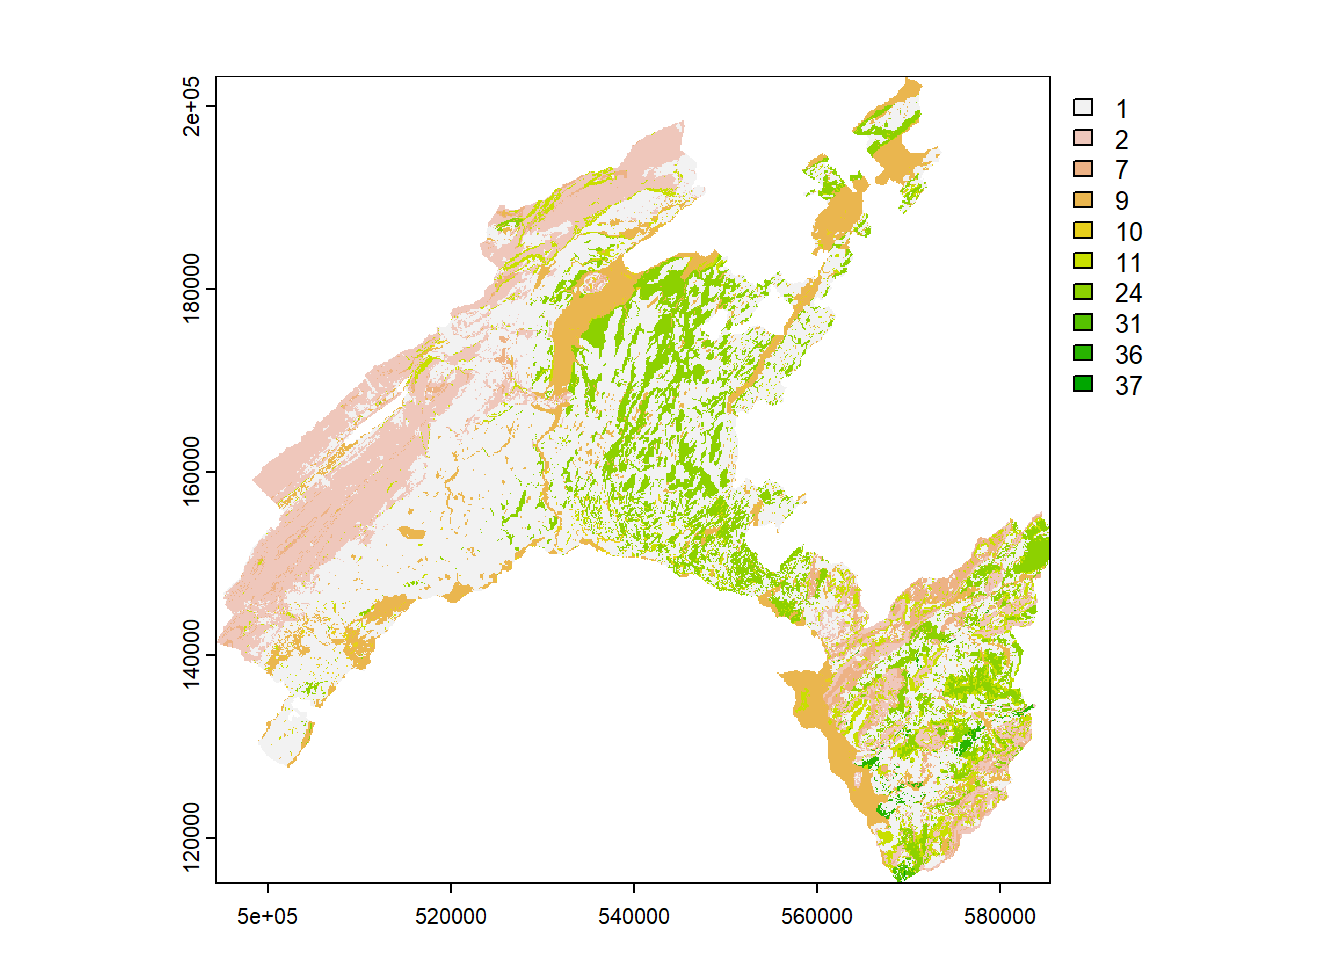
\includegraphics{05-RF_Cl_files/figure-latex/geology-map-1} \end{center}

\begin{Shaded}
\begin{Highlighting}[]
\FunctionTok{plot}\NormalTok{(landCover)}
\end{Highlighting}
\end{Shaded}

\begin{center}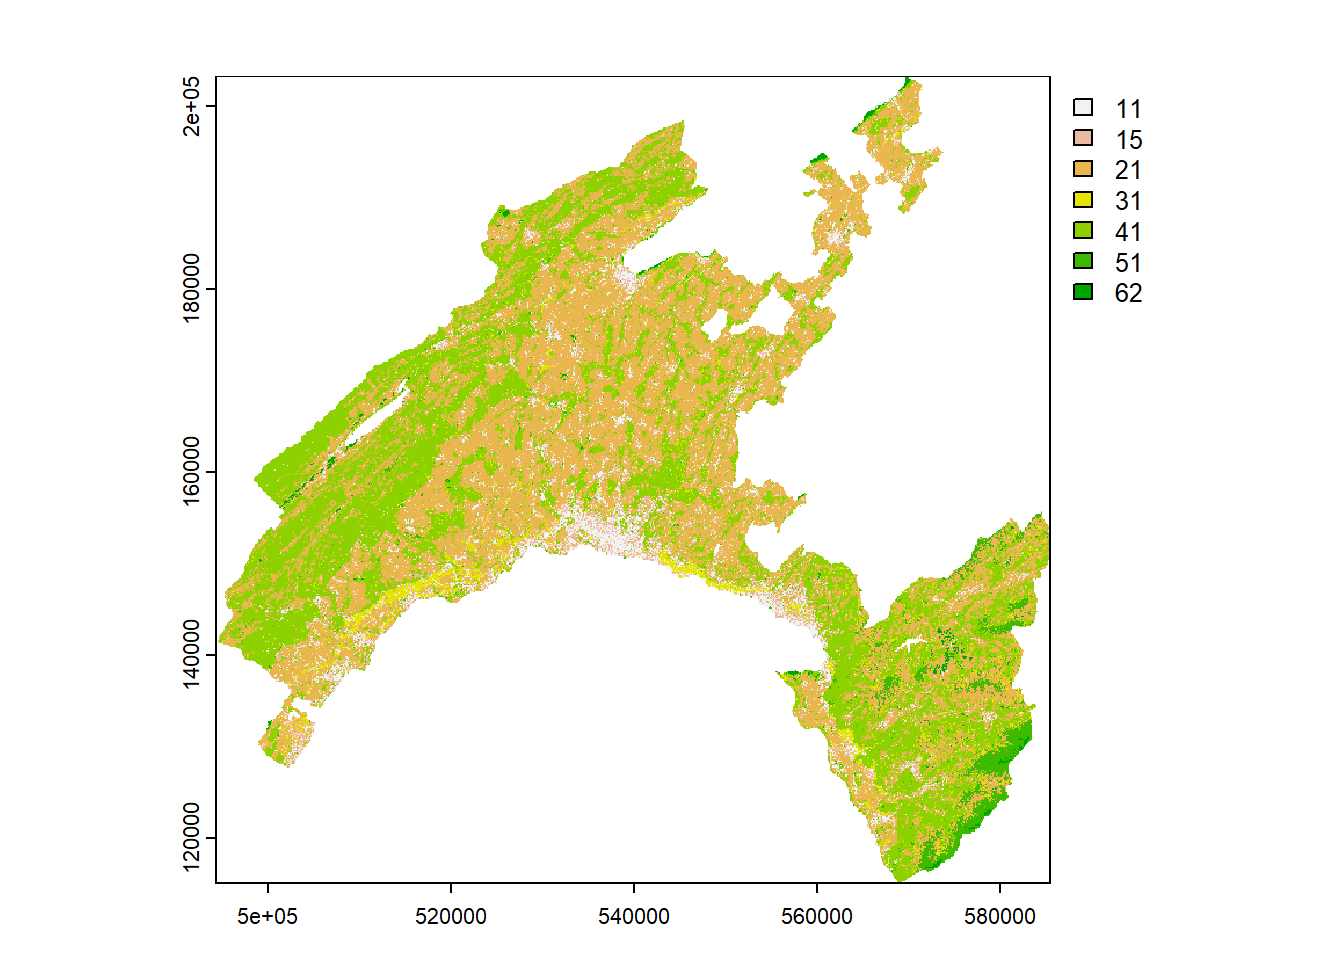
\includegraphics{05-RF_Cl_files/figure-latex/geology-map-2} \end{center}

\begin{figure}

{\centering 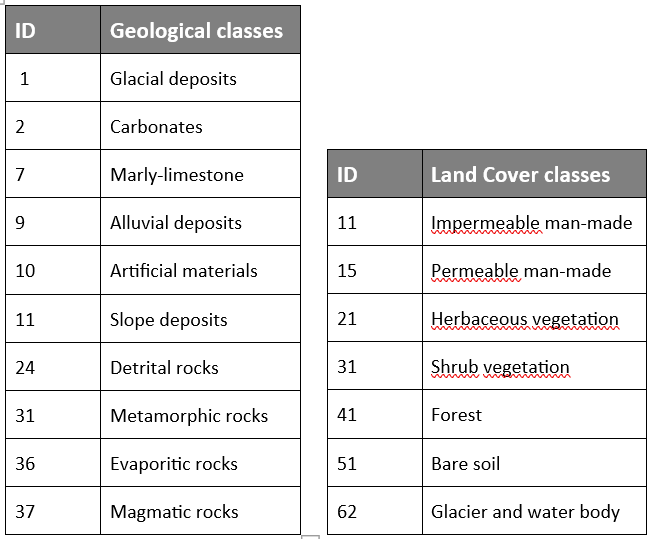
\includegraphics[width=0.8\linewidth,height=0.8\textheight]{data/RF/CatClasses} 

}

\caption{Categorical variables \label{CatClass}}\label{fig:cat-class}
\end{figure}

\newpage

\subsubsection{Extract the values}\label{extract-the-values}

In this step, you will extract the values of the predictors at each location in the landslides (presences and absences) dataset.
The final output represents the input dataset with dependent (LS = landslides) and independent (raster features) variables.

\begin{Shaded}
\begin{Highlighting}[]
\CommentTok{\# Extract values from the raster dataset (features)}
\NormalTok{LS\_input }\OtherTok{\textless{}{-}}\FunctionTok{extract}\NormalTok{(features, LS\_vect, }\AttributeTok{method=}\StringTok{"simple"}\NormalTok{,  }\AttributeTok{xy=}\ConstantTok{TRUE}\NormalTok{)}

\NormalTok{LS\_input}\SpecialCharTok{$}\NormalTok{LS }\OtherTok{\textless{}{-}} \FunctionTok{as.factor}\NormalTok{(LS\_vect}\SpecialCharTok{$}\NormalTok{LS) }\CommentTok{\# add LS}
\FunctionTok{str}\NormalTok{(LS\_input) }\CommentTok{\# explore the dataset}

\CommentTok{\# Remove extra column (ID)}
\NormalTok{LS\_input }\OtherTok{\textless{}{-}}\NormalTok{ LS\_input[,}\DecValTok{2}\SpecialCharTok{:}\FunctionTok{ncol}\NormalTok{(LS\_input)]}
\NormalTok{LS\_input}\OtherTok{\textless{}{-}}\FunctionTok{na.omit}\NormalTok{(LS\_input)}

\CommentTok{\# Explore the newly created input dataset}
\FunctionTok{head}\NormalTok{(LS\_input)}
\FunctionTok{str}\NormalTok{(LS\_input)}
\end{Highlighting}
\end{Shaded}

\subsubsection{Split the input dataset into training and testing}\label{split-the-input-dataset-into-training-and-testing}

A well-established procedure in ML is to split the input dataset into training, validation, and testing.

\begin{itemize}
\tightlist
\item
  The \textbf{training dataset} is needed to calibrate the parameters of the model, which will be used to get predictions on new data.
\item
  The purpose of the \textbf{validation dataset} is to optimize the hyperparameter of the model in the training phase. NB: in RF this subset is represented by the \emph{Out-Of-Bag} (\textbf{OOB})!
\item
  The \textbf{testing dataset} is used in thein the prediction phase: results are predicted over these ``new'' observations (unused before) to provide an unbiased evaluation of the final model and to assess its performance.
\end{itemize}

\begin{Shaded}
\begin{Highlighting}[]
\CommentTok{\# Shuffle the rows}
\FunctionTok{set.seed}\NormalTok{(}\DecValTok{123}\NormalTok{) }\CommentTok{\# to ensure reproducibility }
\NormalTok{LS\_input\_sh}\OtherTok{\textless{}{-}}\NormalTok{LS\_input [}\FunctionTok{sample}\NormalTok{(}\FunctionTok{nrow}\NormalTok{(LS\_input), }\FunctionTok{nrow}\NormalTok{(LS\_input)), ] }

\CommentTok{\# Split the input dataset into training (80\%) and testing (20\%)}
\NormalTok{n }\OtherTok{\textless{}{-}} \FunctionTok{nrow}\NormalTok{ (LS\_input\_sh)}
\FunctionTok{set.seed}\NormalTok{(}\DecValTok{123}\NormalTok{)}
\NormalTok{n\_train }\OtherTok{\textless{}{-}} \FunctionTok{round}\NormalTok{(}\FloatTok{0.80} \SpecialCharTok{*}\NormalTok{ n) }
\NormalTok{train\_indices }\OtherTok{\textless{}{-}} \FunctionTok{sample}\NormalTok{(}\DecValTok{1}\SpecialCharTok{:}\NormalTok{n, n\_train)}

\CommentTok{\# Create indices}
\NormalTok{LS\_train }\OtherTok{\textless{}{-}}\NormalTok{ LS\_input\_sh[train\_indices, ]  }
\NormalTok{LS\_test }\OtherTok{\textless{}{-}}\NormalTok{ LS\_input\_sh[}\SpecialCharTok{{-}}\NormalTok{train\_indices, ]}

\CommentTok{\# Count the number of elements in the two subset: training and testing}
\FunctionTok{count}\NormalTok{(LS\_train)}
\FunctionTok{count}\NormalTok{(LS\_test)}
\end{Highlighting}
\end{Shaded}

\subsubsection{Run Random Forest}\label{run-random-forest}

In RF a subset of the training dataset is generated by bootstrapping (i.e.~random sampling with replacement).
For each subset a decision tree is grown and, at each split, the algorithm randomly selects a number of variables (\texttt{mtry}) and it computes the Gini index to identify the best one.
The process stops when each node contains less than a fixed number of data points.
The main hyperparameters that needs to be defined in RF are \texttt{mtry} and the total number of trees (\texttt{ntrees}).
In this lab we fix these values to 3 and 500, respectively.

The prediction error on the training dataset is finally assessed by evaluating predictions on those observations that were not used in the subset, defined as ``out-of-bag'' (OOB).
This values is used the optimize the values of the hyperparameters, by a trial and error process (that is, trying to minimize the OOB estimate of error rate).

For the computation we introduce here the method proposed by \citet{breiman_random_2001} and implemented in the R package \texttt{randomForest} \citep{RF_library}.

\begin{Shaded}
\begin{Highlighting}[]
\CommentTok{\# Set the seed of R‘s random number generator, }
\DocumentationTok{\#\# this is useful for creating simulations that can be reproduced.}
\FunctionTok{set.seed}\NormalTok{(}\DecValTok{123}\NormalTok{) }

\CommentTok{\# Run RF model}
\NormalTok{RF\_LS}\OtherTok{\textless{}{-}}\FunctionTok{randomForest}\NormalTok{(}\AttributeTok{y=}\NormalTok{LS\_train}\SpecialCharTok{$}\NormalTok{LS, }\AttributeTok{x=}\NormalTok{LS\_train[}\DecValTok{1}\SpecialCharTok{:}\DecValTok{8}\NormalTok{],}\AttributeTok{data=}\NormalTok{LS\_train, }\AttributeTok{ntree=}\DecValTok{500}\NormalTok{, }\AttributeTok{mtry=}\DecValTok{3}\NormalTok{,}\AttributeTok{importance=}\ConstantTok{TRUE}\NormalTok{)}
\end{Highlighting}
\end{Shaded}

\subsubsection{RF main outputs}\label{rf-main-outputs}

Printing the results of RF allows you to gain insight into the outputs of the implemented model, namely the following: a summary of the model hyperparameters, the OOB estimate of error rate, the confusion matrix (in this case a 2x2 matrix used for evaluating the performance of the classification model: 1==presence \emph{vs} 0==absence).

The plot of the error rate is useful to estimate the decreasing values on the OOB and on the predictions (1==presence \emph{vs} 0==absence) over increasing number of trees.

\begin{Shaded}
\begin{Highlighting}[]
\CommentTok{\# Print the model setting}
\FunctionTok{print}\NormalTok{(RF\_LS) }
\end{Highlighting}
\end{Shaded}

\begin{verbatim}
## 
## Call:
##  randomForest(x = LS_train[1:8], y = LS_train$LS, ntree = 500,      mtry = 3, importance = TRUE, data = LS_train) 
##                Type of random forest: classification
##                      Number of trees: 500
## No. of variables tried at each split: 3
## 
##         OOB estimate of  error rate: 16.19%
## Confusion matrix:
##      0    1 class.error
## 0 1681  395   0.1902697
## 1  275 1787   0.1333657
\end{verbatim}

\begin{Shaded}
\begin{Highlighting}[]
\CommentTok{\# Show the predicted probability values}
\NormalTok{RF.predict }\OtherTok{\textless{}{-}} \FunctionTok{predict}\NormalTok{(RF\_LS,}\AttributeTok{type=}\StringTok{"prob"}\NormalTok{)}
\FunctionTok{head}\NormalTok{(RF.predict) }\CommentTok{\# 0 = absence ; 1 = presence}
\end{Highlighting}
\end{Shaded}

\begin{verbatim}
##               0         1
## 1447 0.20108696 0.7989130
## 671  0.01463415 0.9853659
## 1121 0.22099448 0.7790055
## 4443 0.79207921 0.2079208
## 4032 0.21500000 0.7850000
## 2075 0.16666667 0.8333333
\end{verbatim}

\begin{Shaded}
\begin{Highlighting}[]
\CommentTok{\# Plot the OOB error rate}
\FunctionTok{plot}\NormalTok{(RF\_LS)  }
\FunctionTok{legend}\NormalTok{(}\AttributeTok{x=}\StringTok{"topright"}\NormalTok{, }\AttributeTok{legend=}\FunctionTok{c}\NormalTok{(}\StringTok{"perd 0"}\NormalTok{, }\StringTok{"pred 1"}\NormalTok{, }\StringTok{"OOB error"}\NormalTok{), }
 \AttributeTok{col=}\FunctionTok{c}\NormalTok{(}\StringTok{"red"}\NormalTok{, }\StringTok{"green"}\NormalTok{, }\StringTok{"black"}\NormalTok{), }\AttributeTok{lty=}\DecValTok{1}\SpecialCharTok{:}\DecValTok{2}\NormalTok{, }\AttributeTok{cex=}\FloatTok{0.8}\NormalTok{)}
\end{Highlighting}
\end{Shaded}

\begin{center}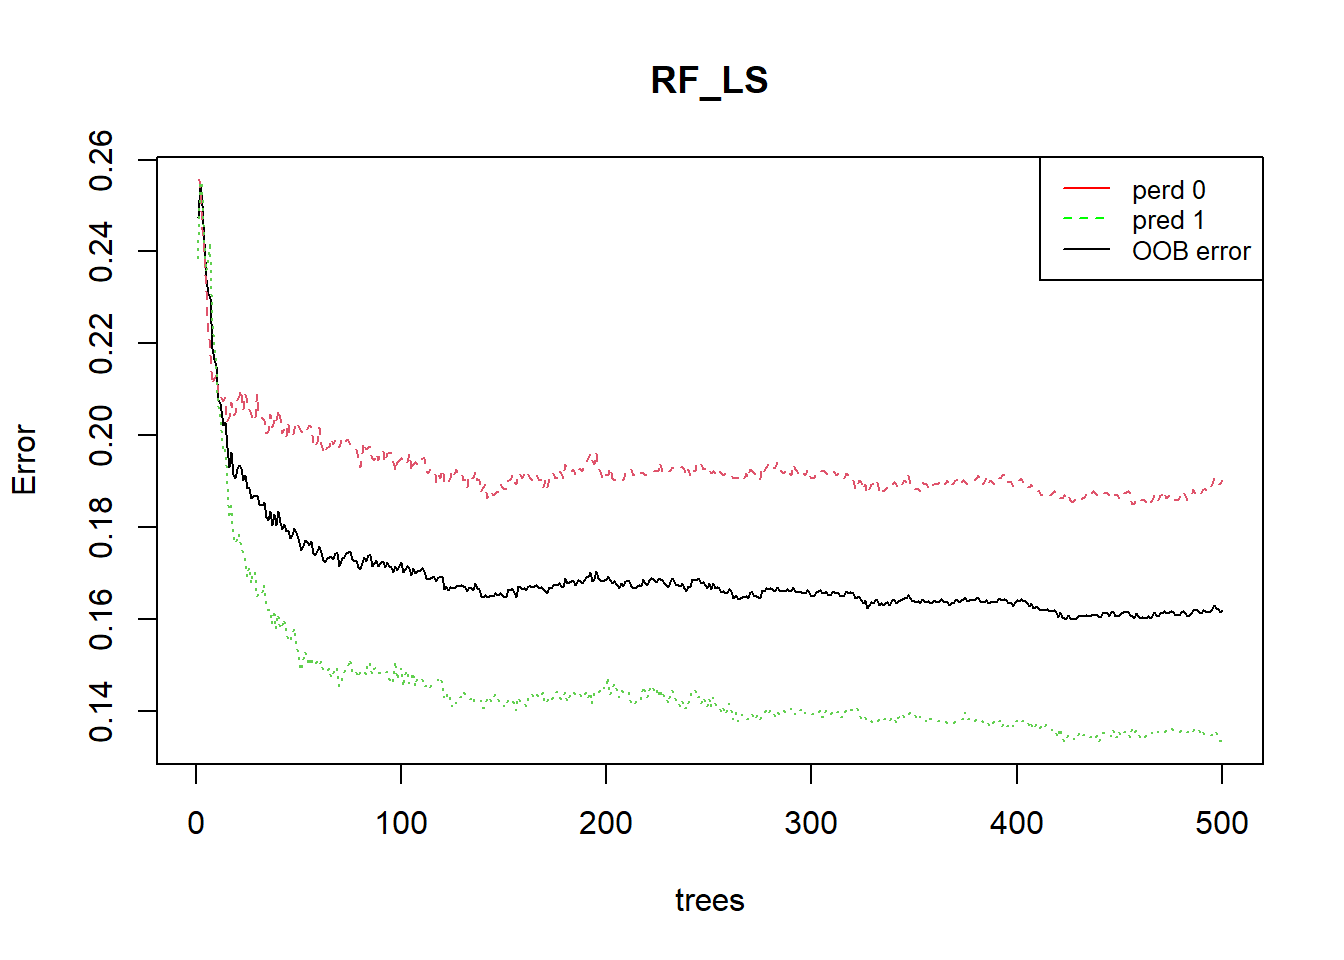
\includegraphics{05-RF_Cl_files/figure-latex/RF-outputs-1} \end{center}

\subsubsection{Model evaluation}\label{model-evaluation}

The prediction capability of the implemented RF model can be evaluated by predicting the results over previously unseen data, that is the testing dataset.
The \emph{Area Under the ``Receiver Operating Characteristic (ROC)'' Curve} (\textbf{AUC}) represents the evaluation score used here as indicator of the goodness of the model in classifying areas more susceptible to landslides.
The ROC curve is a graphical technique based on the plot of the percentage of correct classification (the true positives rate) against the false positives rate (occurring when an outcome is incorrectly predicted as belonging to the class ``1'' when it actually belongs to the class ``0''), evaluates for many thresholds.
The AUC value lies between 0.5, denoting a bad classifier, and 1, denoting an excellent classifier, which, on the other hand, can indicate overfitting.

\begin{Shaded}
\begin{Highlighting}[]
\CommentTok{\# Make predictions on the testing dataset}
\NormalTok{RFpred\_test }\OtherTok{\textless{}{-}} \FunctionTok{predict}\NormalTok{(}\AttributeTok{object =}\NormalTok{ RF\_LS, }\AttributeTok{newdata =}\NormalTok{ LS\_test, }\AttributeTok{type=}\StringTok{"prob"}\NormalTok{)}

\CommentTok{\# Make predictions on the validation dataset (taining using the Out{-}of{-}bag)}
\NormalTok{RFpred\_oob }\OtherTok{\textless{}{-}} \FunctionTok{predict}\NormalTok{(}\AttributeTok{object =}\NormalTok{ RF\_LS, }\AttributeTok{newdata =}\NormalTok{ LS\_train, }\AttributeTok{type=}\StringTok{"prob"}\NormalTok{, }\AttributeTok{OOB=}\ConstantTok{TRUE}\NormalTok{)}

\NormalTok{roc\_test }\OtherTok{\textless{}{-}} \FunctionTok{roc}\NormalTok{(LS\_test}\SpecialCharTok{$}\NormalTok{LS, RFpred\_test[,}\DecValTok{2}\NormalTok{])}
\NormalTok{roc\_oob }\OtherTok{\textless{}{-}} \FunctionTok{roc}\NormalTok{(LS\_train}\SpecialCharTok{$}\NormalTok{LS, RFpred\_oob[,}\DecValTok{2}\NormalTok{])}

\FunctionTok{plot.new}\NormalTok{()}
\FunctionTok{plot}\NormalTok{(}\DecValTok{1}\SpecialCharTok{{-}}\NormalTok{roc\_test}\SpecialCharTok{$}\NormalTok{specificities, roc\_test}\SpecialCharTok{$}\NormalTok{sensitivities, }\AttributeTok{type =} \StringTok{\textquotesingle{}l\textquotesingle{}}\NormalTok{, }\AttributeTok{col =} \StringTok{\textquotesingle{}blue\textquotesingle{}}\NormalTok{,  }\AttributeTok{xlab =} \StringTok{"False positive rate"}\NormalTok{, }\AttributeTok{ylab =} \StringTok{"True positive rate"}\NormalTok{)}
\FunctionTok{lines}\NormalTok{(}\DecValTok{1}\SpecialCharTok{{-}}\NormalTok{roc\_oob}\SpecialCharTok{$}\NormalTok{specificities, roc\_oob}\SpecialCharTok{$}\NormalTok{sensitivities, }\AttributeTok{type =} \StringTok{\textquotesingle{}l\textquotesingle{}}\NormalTok{, }\AttributeTok{col =} \StringTok{\textquotesingle{}red\textquotesingle{}}\NormalTok{)}
\end{Highlighting}
\end{Shaded}

\begin{center}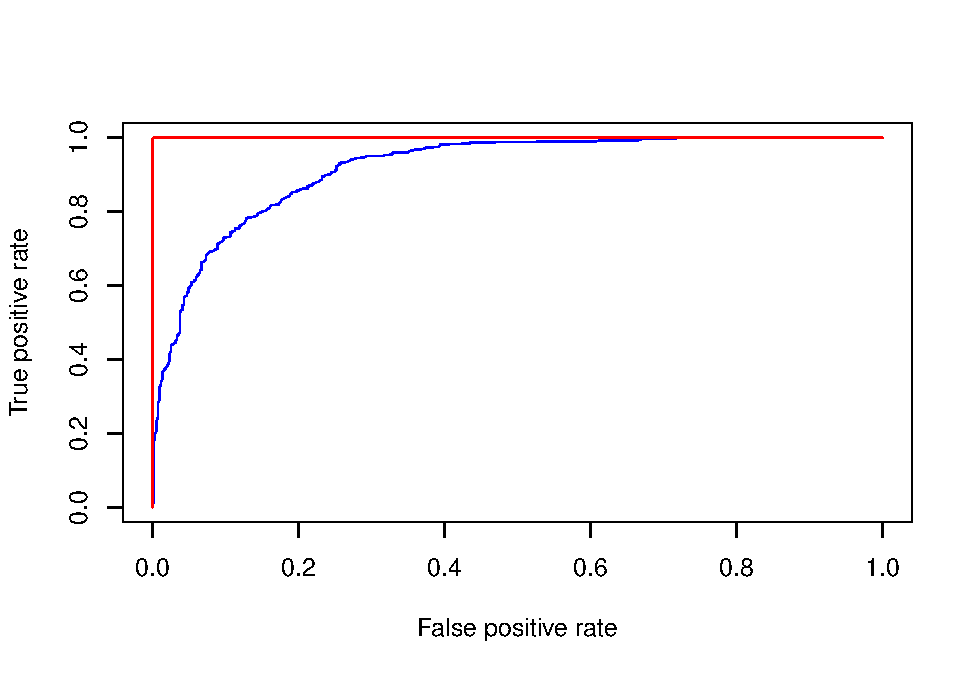
\includegraphics{05-RF_Cl_files/figure-latex/RF-val-1} \end{center}

\begin{Shaded}
\begin{Highlighting}[]
\CommentTok{\# Print AUC values}
\NormalTok{roc\_test}
\NormalTok{roc\_oob}
\end{Highlighting}
\end{Shaded}

\subsection{Susceptibility mapping}\label{susceptibility-mapping}

You have now all the elements necessary to elaborate the final landslide susceptibility map.
This can be achieved by making predictions (of presence only) based on the values of the predictor variables, which are stored into the multiple-raster named \emph{features}, created above.

\begin{Shaded}
\begin{Highlighting}[]
\CommentTok{\# Convert the input multiple raster to data frame }
\NormalTok{features\_df}\OtherTok{\textless{}{-}}\FunctionTok{as.data.frame}\NormalTok{(features, }\AttributeTok{xy=}\ConstantTok{TRUE}\NormalTok{, }\AttributeTok{na.rm=}\ConstantTok{TRUE}\NormalTok{) }

\CommentTok{\# Predict results of RF (probability of fires presence: index = 2) to the feature space }
\DocumentationTok{\#\# this operation can take several minuts to run!}
\NormalTok{scp\_map}\OtherTok{\textless{}{-}}\FunctionTok{predict}\NormalTok{(}\AttributeTok{object =}\NormalTok{ RF\_LS, }\AttributeTok{newdata =}\NormalTok{ features\_df, }\AttributeTok{type=}\StringTok{"prob"}\NormalTok{, }\AttributeTok{index=}\DecValTok{2}\NormalTok{) }

\NormalTok{scp\_df}\OtherTok{=}\FunctionTok{as.data.frame}\NormalTok{(scp\_map) }\CommentTok{\# convert to data frame}
\CommentTok{\# get coordinates }
\NormalTok{scp\_df}\SpecialCharTok{$}\NormalTok{X}\OtherTok{=}\NormalTok{features\_df}\SpecialCharTok{$}\NormalTok{x}
\NormalTok{scp\_df}\SpecialCharTok{$}\NormalTok{Y}\OtherTok{=}\NormalTok{features\_df}\SpecialCharTok{$}\NormalTok{y}

\CommentTok{\# Convert to raster the probability to get a landslide}
\DocumentationTok{\#\# 3=X, 4=Y, 2=probability of presence (1)}
\NormalTok{scp\_rast}\OtherTok{=}\FunctionTok{rast}\NormalTok{(scp\_df[,}\FunctionTok{c}\NormalTok{(}\DecValTok{3}\NormalTok{,}\DecValTok{4}\NormalTok{,}\DecValTok{2}\NormalTok{)],}\AttributeTok{type=}\StringTok{"xyz"}\NormalTok{)}
\FunctionTok{summary}\NormalTok{(scp\_rast)}
\FunctionTok{plot}\NormalTok{(scp\_rast)}
\end{Highlighting}
\end{Shaded}

\begin{center}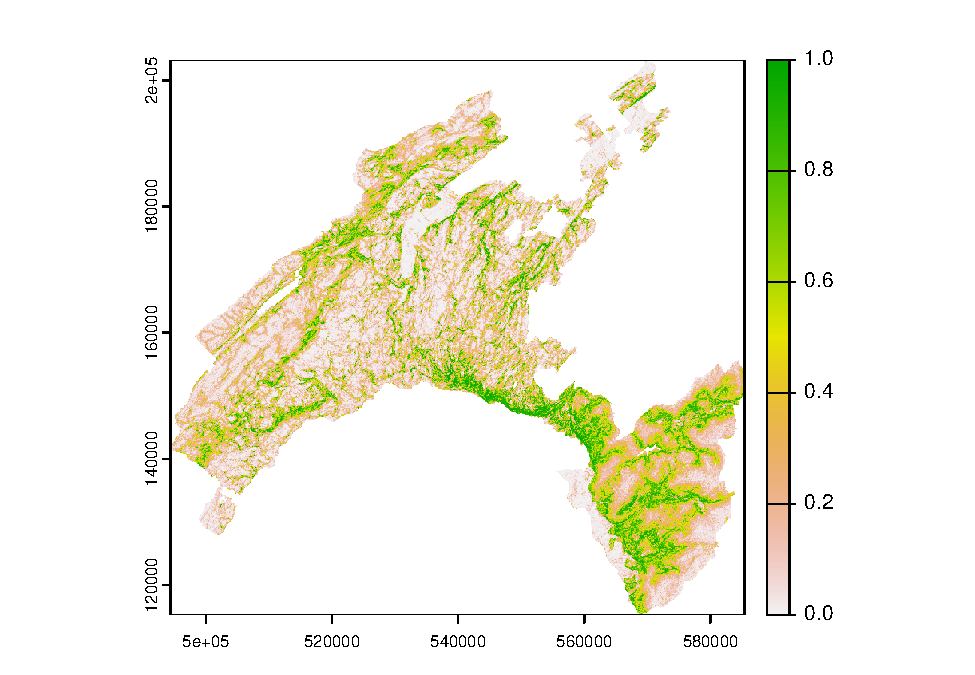
\includegraphics{05-RF_Cl_files/figure-latex/Scp-map-1} \end{center}

\begin{Shaded}
\begin{Highlighting}[]
\CommentTok{\# Save all outputs}
\DocumentationTok{\#\# this operation can take several minuts to run!}
\FunctionTok{save.image}\NormalTok{(}\AttributeTok{file=}\StringTok{"LSM\_RF.RData"}\NormalTok{)}

\CommentTok{\# Export susceptibility map as raster}
\FunctionTok{writeRaster}\NormalTok{(scp\_rast,}\StringTok{"Susceptibility\_LSmap.tif"}\NormalTok{,}\AttributeTok{overwrite=}\NormalTok{T) }
\end{Highlighting}
\end{Shaded}

\subsubsection{Class intervals for decision maker}\label{class-intervals-for-decision-maker}

What can you say by looking at this map?
Actually a risk heat map like this provide a data visualization tool for communicating the level for a specific risk to occur.
These maps helps authorities to identify and prioritize the risks associated with a given hazard.

Normally an authority (i.e., a decision maker) prioritize its efforts based on the available resources it has.
So, it can be more useful to detect the areas with the highest probability of burning based on certain intervals (i.e., breaks).
The authority can thus concentrate its resources for preventive actions on a given threshold (such as 5\%, 10\%, or 20\%) of the area with the highest probability of burning, instead of concentrates on the areas with a ``stochastic'' output probability value of 0.8 (for example).

\paragraph{Equal intervals}\label{equal-intervals}

Susceptibility maps are based on equal intervals, five classes (each 20\%) in this case.

\begin{Shaded}
\begin{Highlighting}[]
\FunctionTok{library}\NormalTok{(}\StringTok{"RColorBrewer"}\NormalTok{)}
\FunctionTok{plot}\NormalTok{(scp\_rast, }\AttributeTok{xlab =} \StringTok{"East [m]"}\NormalTok{, }\AttributeTok{ylab =} \StringTok{"North [m]"}\NormalTok{, }\AttributeTok{main =} \StringTok{"Landslides susceptibility map"}\NormalTok{, }\AttributeTok{col =} \FunctionTok{rev}\NormalTok{(}\FunctionTok{c}\NormalTok{(}\StringTok{\textquotesingle{}\#a50026\textquotesingle{}}\NormalTok{,}\StringTok{\textquotesingle{}\#d73027\textquotesingle{}}\NormalTok{,}\StringTok{\textquotesingle{}\#f46d43\textquotesingle{}}\NormalTok{,}\StringTok{\textquotesingle{}\#fdae61\textquotesingle{}}\NormalTok{,}\StringTok{\textquotesingle{}\#fee08b\textquotesingle{}}\NormalTok{,}\StringTok{\textquotesingle{}\#d9ef8b\textquotesingle{}}\NormalTok{)))}
\end{Highlighting}
\end{Shaded}

\begin{center}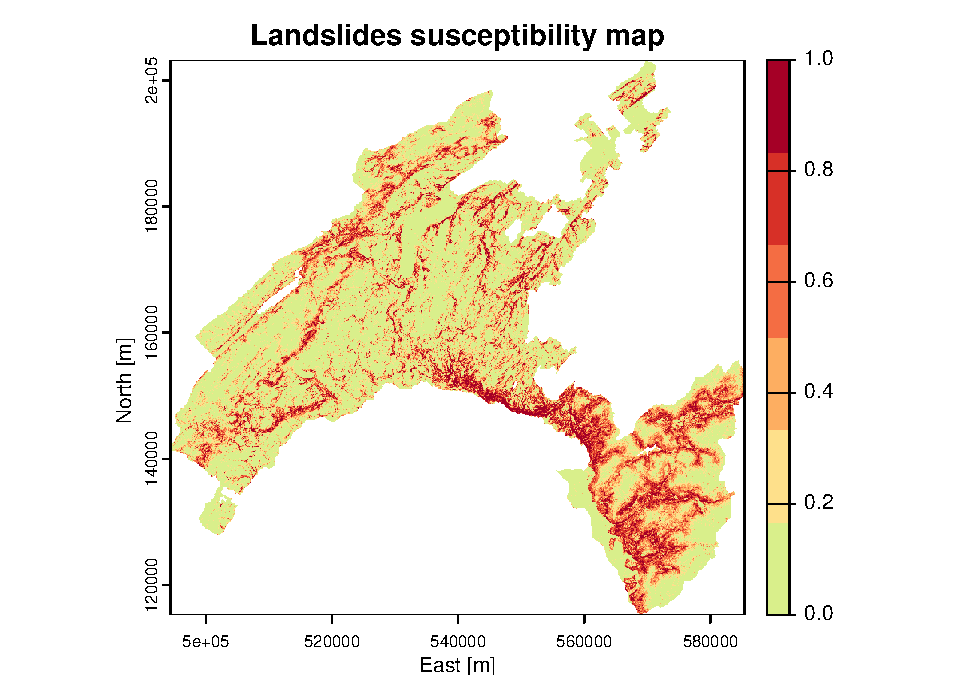
\includegraphics{05-RF_Cl_files/figure-latex/equal-interval-map-1} \end{center}

\paragraph{Quartile}\label{quartile}

Breaks are chosen based on the summary statics: these values corresponds to the quartiles of the p-value distribution (values divided into four equal partitions).

\begin{Shaded}
\begin{Highlighting}[]
\NormalTok{brk}\OtherTok{\textless{}{-}}\FunctionTok{c}\NormalTok{(}\DecValTok{0}\NormalTok{, }\FloatTok{0.03}\NormalTok{, }\FloatTok{0.14}\NormalTok{, }\FloatTok{0.43}\NormalTok{, }\DecValTok{1}\NormalTok{) }

\FunctionTok{plot}\NormalTok{(scp\_rast, }\AttributeTok{xlab =} \StringTok{"East [m]"}\NormalTok{, }\AttributeTok{ylab =} \StringTok{"North [m]"}\NormalTok{, }
     \AttributeTok{main =} \StringTok{"Landslides susceptibility map"}\NormalTok{, }
     \AttributeTok{col =} \FunctionTok{rev}\NormalTok{(}\FunctionTok{c}\NormalTok{(}\StringTok{"brown"}\NormalTok{, }\StringTok{"orange"}\NormalTok{, }\StringTok{"yellow"}\NormalTok{, }\StringTok{"grey"}\NormalTok{)), }\AttributeTok{breaks=}\NormalTok{brk) }
\end{Highlighting}
\end{Shaded}

\begin{center}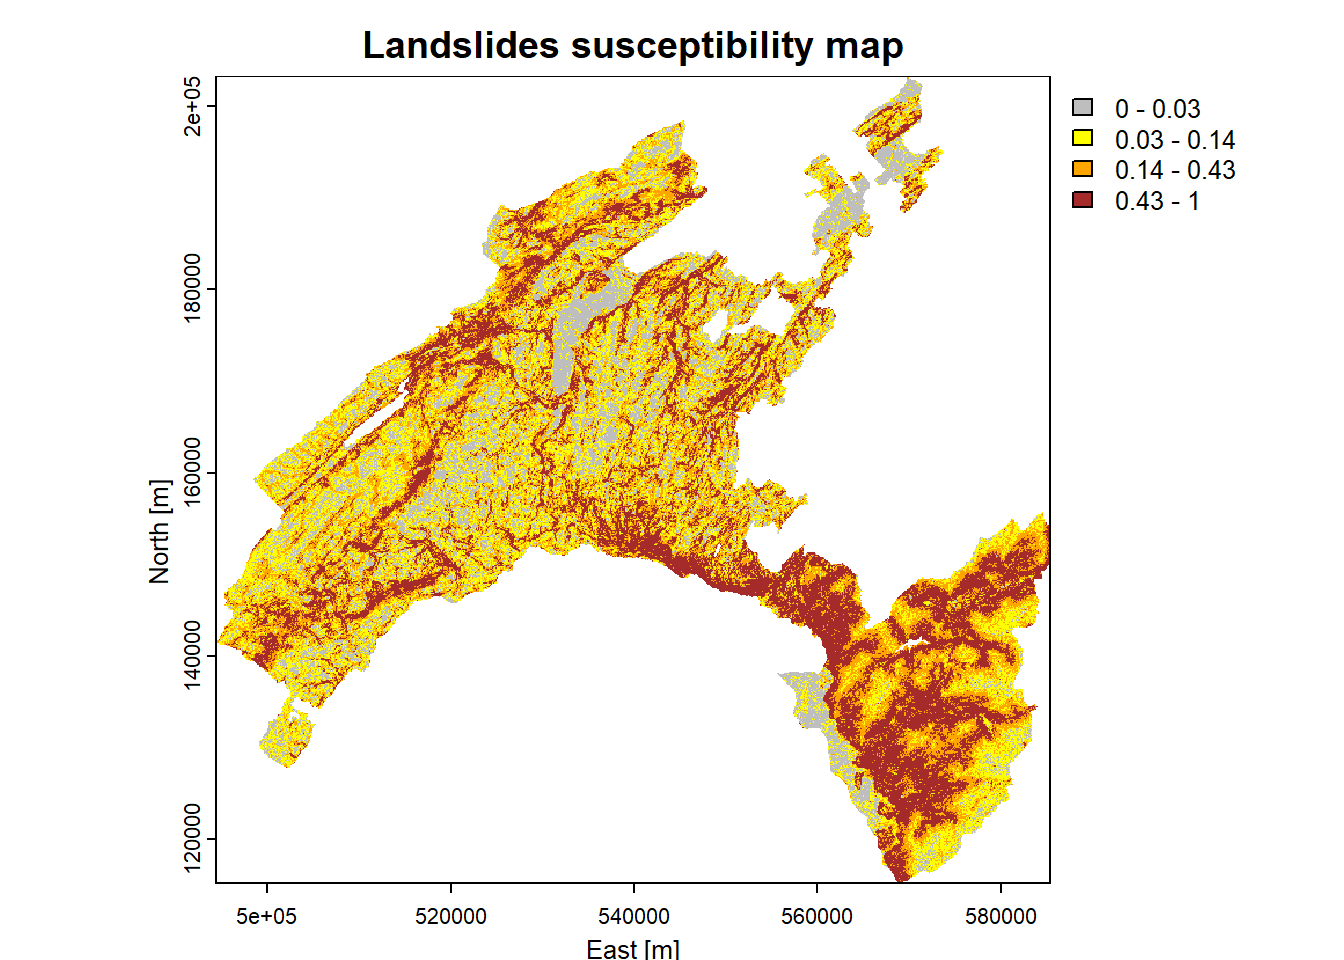
\includegraphics{05-RF_Cl_files/figure-latex/quartile-map-1} \end{center}

\paragraph{Percentiles}\label{percentiles}

Breaks are chosen based on well-established percentile classes.
For exaple, in this case the 20th percentile correspond to the p-value below wich the 25\% of the observation lie, while the 95th can be interpreted as the p-value above which the complementary 5\% of the observation lie.
The legend show the p-values correspondig to the percentile classes indicated below.

\begin{Shaded}
\begin{Highlighting}[]
\CommentTok{\# Output predicted values are transformed to a vector}
\NormalTok{pred.vect }\OtherTok{\textless{}{-}} \FunctionTok{as.vector}\NormalTok{(scp\_map[, }\DecValTok{2}\NormalTok{])}

\CommentTok{\# The function "quantile" is used to fix classes}
\NormalTok{qtl.pred }\OtherTok{\textless{}{-}} \FunctionTok{quantile}\NormalTok{(pred.vect, }\AttributeTok{probs=}\FunctionTok{c}\NormalTok{(}\FloatTok{0.25}\NormalTok{,}\FloatTok{0.5}\NormalTok{,}\FloatTok{0.75}\NormalTok{,}\FloatTok{0.85}\NormalTok{,}\FloatTok{0.95}\NormalTok{), }\AttributeTok{na.rm =} \ConstantTok{TRUE}\NormalTok{)}
\NormalTok{qtl.pred}
\end{Highlighting}
\end{Shaded}

\begin{verbatim}
##   25%   50%   75%   85%   95% 
## 0.046 0.166 0.448 0.614 0.832
\end{verbatim}

\begin{Shaded}
\begin{Highlighting}[]
\CommentTok{\# and then extract the corresponding values}
\NormalTok{qtl.int}\OtherTok{\textless{}{-}} \FunctionTok{c}\NormalTok{(}\DecValTok{0}\NormalTok{,}\FloatTok{0.03}\NormalTok{,}\FloatTok{0.14}\NormalTok{,}\FloatTok{0.42}\NormalTok{,}\FloatTok{0.6}\NormalTok{,}\FloatTok{0.82}\NormalTok{,}\DecValTok{1}\NormalTok{)}
\FunctionTok{plot}\NormalTok{(scp\_rast, }\AttributeTok{xlab =} \StringTok{"East [m]"}\NormalTok{, }\AttributeTok{ylab =} \StringTok{"North [m]"}\NormalTok{, }
     \AttributeTok{main =} \StringTok{"Landslides susceptibility map"}\NormalTok{, }
     \AttributeTok{col =} \FunctionTok{rev}\NormalTok{(}\FunctionTok{c}\NormalTok{(}\StringTok{"brown"}\NormalTok{, }\StringTok{"red"}\NormalTok{, }\StringTok{"orange"}\NormalTok{,}\StringTok{"yellow"}\NormalTok{, }\StringTok{"green"}\NormalTok{, }\StringTok{"grey"}\NormalTok{)), }\AttributeTok{breaks=}\NormalTok{qtl.int)}
\end{Highlighting}
\end{Shaded}

\begin{center}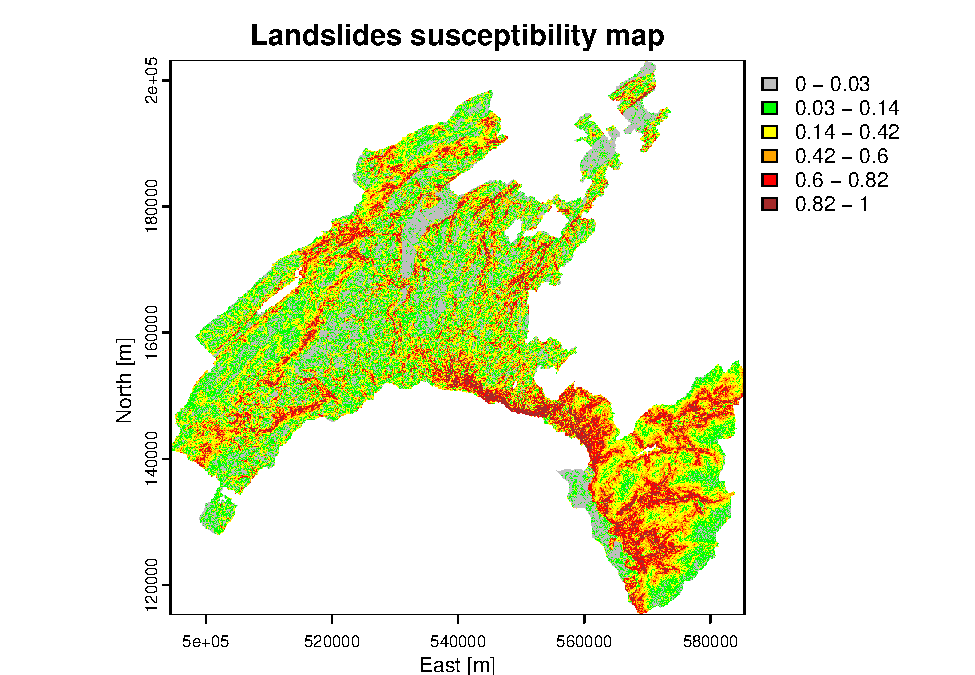
\includegraphics{05-RF_Cl_files/figure-latex/percentile-map-1} \end{center}

\subsection{Conclusions and further analyses}\label{conclusions-and-further-analyses-2}

This exercise allowed you to familiarize with Random Forest, by the proposed application about landslides susceptibility mapping and variables importance assessment.

To ensure that everything is perfectly clear, we propose you to \textbf{answer the following questions}.

\begin{enumerate}
\def\labelenumi{\arabic{enumi})}
\item
  Why is it important to implement the pseudo-absences, other that the presences (i.e., the observations) in a data-driven modelization?
\item
  What is the difference between a numerical and a categorical variable?
  Give some examples of both types.
  Why RF can handle directly native categorical variables?
  Is it the same for other algorithms (like logistic regression or neural network)?
\item
  Which is the values of the OOB estimate error rate of your model?
  Which parameters you can change to try to reduce it?
  Be brave and do it (i.e., change the values for \emph{ntree} and \emph{mtry,} than analyse which values for the AUC you obtain and which model perform better.
\end{enumerate}

\section{Interpretability \& Explainability with Random Forest}\label{local-rf}

In the world of machine learning, interpretability and explainability are two therms commonly used to describe the extent to which an algorithm's behavior can be understood.
The distinction between them lies in their focus and depth.
We can say that interpretability focuses on understanding the inner workings of the models, while explainability focuses on explaining the decisions made.
Define if an algorithm is interpretable or explainable depend on different factors as described below.

\textbf{Model complexity} -- When dealing with intricate models like Random Forest (with tens of variables and thousands of trees), up to deep neural networks, interpretability becomes challenging due to their complexity and the interplay among their components.
In such scenarios, explainability proves to be a more practical approach, as it focuses on clarifying decisions rather than delving into the complexities of the algorithm.

\textbf{Communication} -- In terms of audience and purpose, interpretability primarily concerns machine learning specialists , whereas explainability targets end users seeking to grasp model decisions.
Consequently, explainability necessitates a more straightforward and intuitive communication of information.

While Random Forest (RF) is a powerful algorithm and often yield high accuracy, interpretability can be challenging due to its complex structure and the high number of tress.
However, the following techniques can enhance the interpretability and explainability of RF models.

\begin{itemize}
\item
  \textbf{Interpretability} -- A \emph{surrogate model}, such as a single decision tree, can approximate the predictions of a more complex model like a RF, which is composed of thousands of decision trees.
  The surrogate model is more interpretable and helps in understanding the general rules that RF tipically follows.
\item
  \textbf{Explainability} -- Examining \emph{feature importance scores}, which measure the contribution of each variable to the model's predictions, allows us to identify the most influential variables in the model's decisions.
  In addition, \emph{partial dependence plots} enable us to visualize how changes in a variable influence the model's predictions, making this tool useful for interpreting the global effects of predictors across the entire dataset.
\end{itemize}

\subsection{Aim of the present lab}\label{aim-of-the-present-lab}

In this computing lab you will work with the outputs of RF resulting from the previous lab on landslides susceptibility map.

\begin{itemize}
\item
  Firstly, we will explore the relative importance of the predictor variables (feature importance scores) , and their relative probability of prediction success (partial dependence plots).
  These are the core of explainability in RF.
\item
  In the second part, we will apply a local version of RF (named ``\emph{Geographical Random Forest}'') to analyse the spatial heterogeneity of the local variable importance.
  This will help to deep our understanding of the influence of the predictor variable explored locally,
\end{itemize}

\subsection{Computing lab: Understanding Random Forest Models}\label{computing-lab-understanding-random-forest-models}

\subsubsection{Re-load libraries and workspace}\label{re-load-libraries-and-workspace}

If you have quit the workspace where you have run the RF model for landslide susceptibility mapping, you need to load it again in this new project.
Loading the workspace refers to the action of restoring the saved state of R environment.
When you save your workspace in R, it typically includes all the objects (such as variables, functions, data frames, etc.) that are currently present in your R session.
Loading the workspace means to restore this saved state, bringing back all the previously saved objects into your current R session.

\begin{verbatim}
##  [1] "RColorBrewer" "tidyr"        "randomForest" "classInt"     "plotROC"     
##  [6] "ggplot2"      "pROC"         "dplyr"        "readr"        "foreign"     
## [11] "terra"        "stats"        "graphics"     "grDevices"    "utils"       
## [16] "datasets"     "methods"      "base"
\end{verbatim}

\subsubsection{Surrogate model}\label{surrogate-model}

Although machine learning algorithms are often considered as a black box, with RF is possible to plot a sample tree (selected randomly) to analyse its structure and investigate how decisions have been made.

\begin{Shaded}
\begin{Highlighting}[]
\FunctionTok{library}\NormalTok{(}\StringTok{"party"}\NormalTok{)}

\NormalTok{x }\OtherTok{\textless{}{-}} \FunctionTok{ctree}\NormalTok{(LS}\SpecialCharTok{\textasciitilde{}}\NormalTok{., }\AttributeTok{data=}\NormalTok{LS\_train)}
\FunctionTok{plot}\NormalTok{(x, }\AttributeTok{type=}\StringTok{"simple"}\NormalTok{)}
\end{Highlighting}
\end{Shaded}

\subsubsection{Features importance score}\label{features-importance-score}

RF provides two scores allowing to assess the importance of each variables in the model: the Mean Decrease in Accuracy (MDA), and the mean decrease in Gini index.
The MDA indicates how much the tree nodes that use a given variable enable reducing the mean-square errors evaluated on the Out-Of-Bag and across all the trees.
The Gini index measures the probability of incorrectly classifying a randomly chosen element in a dataset if that element were classified based on the distribution of classes in a particular node.
The relative importance of the predictor variables can be ranked based on the increasing values of both these scores: the higher the value, the more important the variable.

\begin{Shaded}
\begin{Highlighting}[]
\CommentTok{\# Display the plot with the relative importance of each variable}
\FunctionTok{importance}\NormalTok{(RF\_LS)}
\FunctionTok{varImpPlot}\NormalTok{(RF\_LS)}
\end{Highlighting}
\end{Shaded}

\begin{center}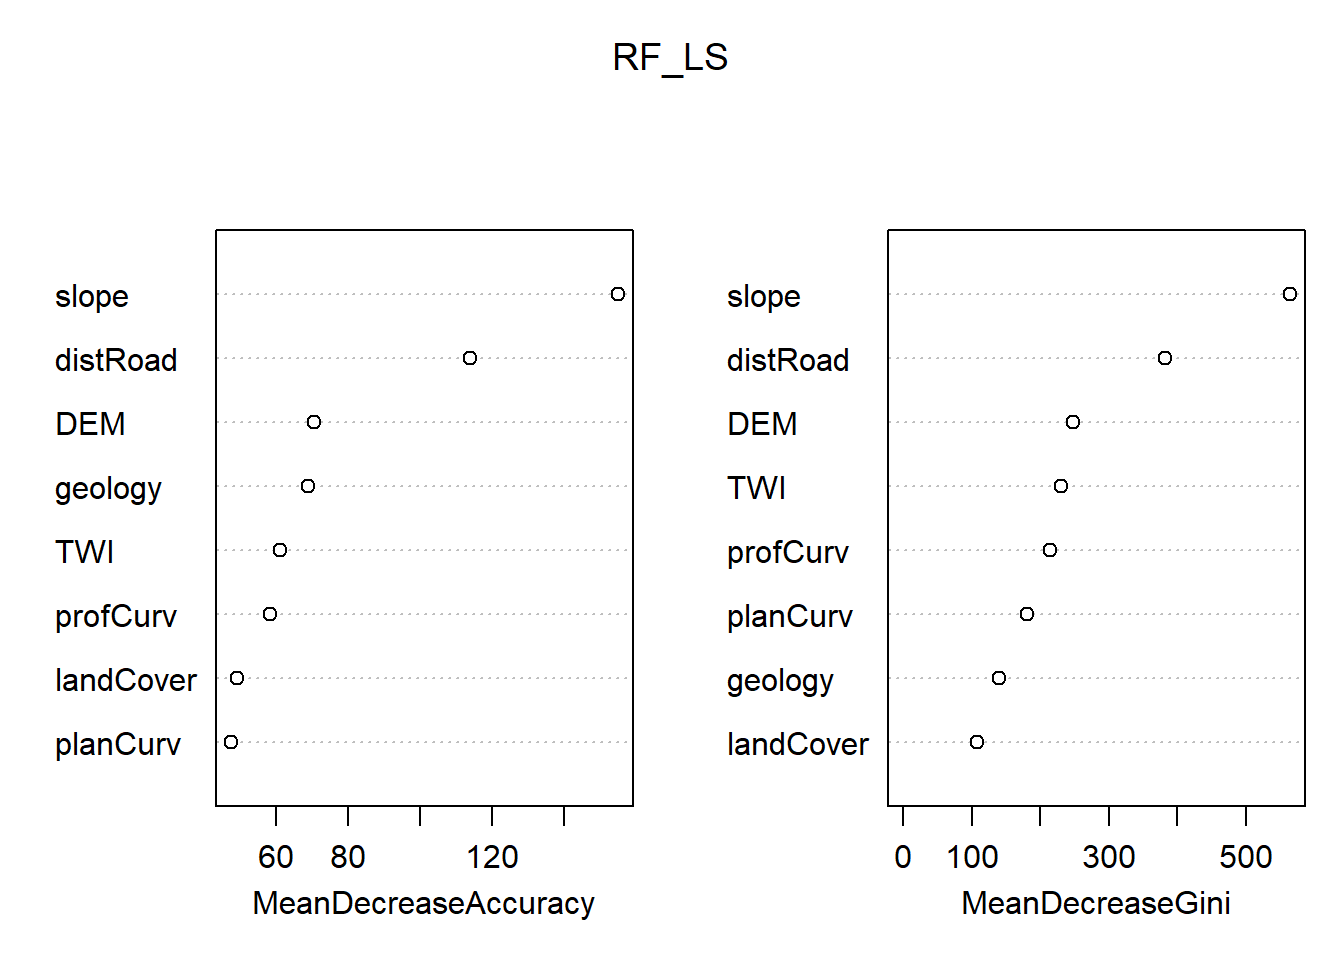
\includegraphics{06-Exp_RF_files/figure-latex/var-imp-1} \end{center}

\subsubsection{Partial dependence plot}\label{partial-dependence-plot}

The Partial Dependence Plot (PDP) allows us to estimate, for each single variable, the relative probability of prediction success over different ranges of values.
PDP provides a graphical depiction of the marginal effect of each variable on the class probability over different ranges of continuous or discrete values.
Positive values are associated with the probability of occurrence of the phenomena (i.e., landslides presence), while negative vales indicate its absence.

\begin{Shaded}
\begin{Highlighting}[]
\CommentTok{\#Compute PDP for all the predictor variables }

\CommentTok{\# Slope}
\FunctionTok{partialPlot}\NormalTok{(RF\_LS, LS\_train, }\AttributeTok{x.var =}\NormalTok{ slope, }\AttributeTok{rug =} \ConstantTok{TRUE}\NormalTok{, }
            \AttributeTok{which.class =}\NormalTok{ RF\_LS}\SpecialCharTok{$}\NormalTok{classes[}\DecValTok{2}\NormalTok{],}\AttributeTok{xlab=} \StringTok{"Slope [°]"}\NormalTok{, }
            \AttributeTok{main =} \StringTok{""}\NormalTok{, }\AttributeTok{ylab =} \StringTok{"PDP"}\NormalTok{)}
\end{Highlighting}
\end{Shaded}

\begin{center}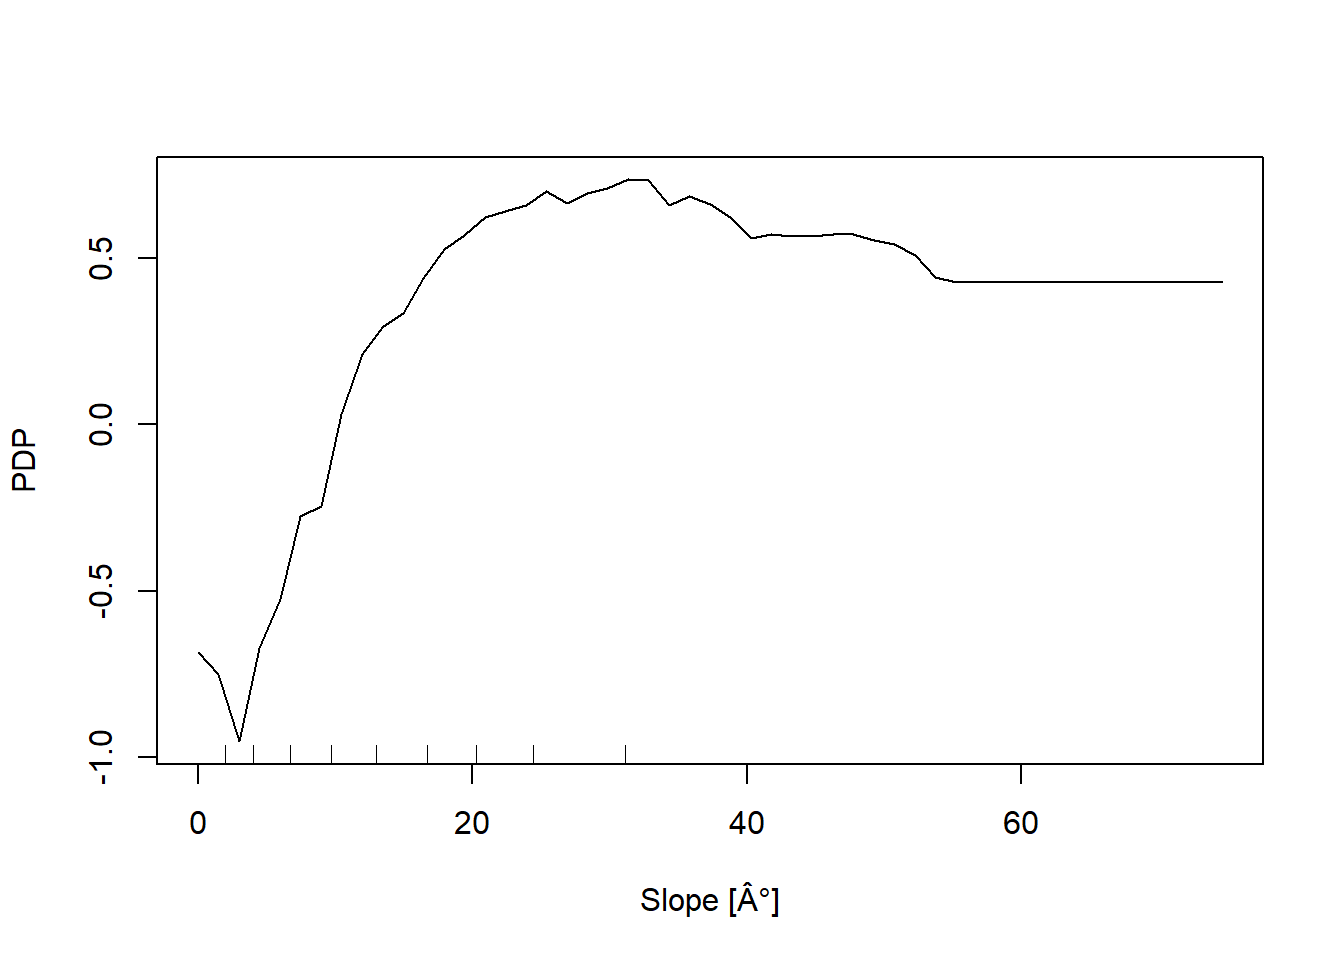
\includegraphics{06-Exp_RF_files/figure-latex/par-plot-1} \end{center}

\begin{Shaded}
\begin{Highlighting}[]
\CommentTok{\# Elevation}
\FunctionTok{partialPlot}\NormalTok{(RF\_LS, LS\_train ,}\AttributeTok{x.var =}\NormalTok{ DEM, }\AttributeTok{rug =} \ConstantTok{TRUE}\NormalTok{, }
            \AttributeTok{which.class =}\NormalTok{ RF\_LS}\SpecialCharTok{$}\NormalTok{classes[}\DecValTok{2}\NormalTok{],}\AttributeTok{xlab=} \StringTok{"Elevation [m]"}\NormalTok{, }
            \AttributeTok{main =} \StringTok{""}\NormalTok{,}\AttributeTok{ylab =} \StringTok{"PDP"}\NormalTok{)}
\end{Highlighting}
\end{Shaded}

\begin{center}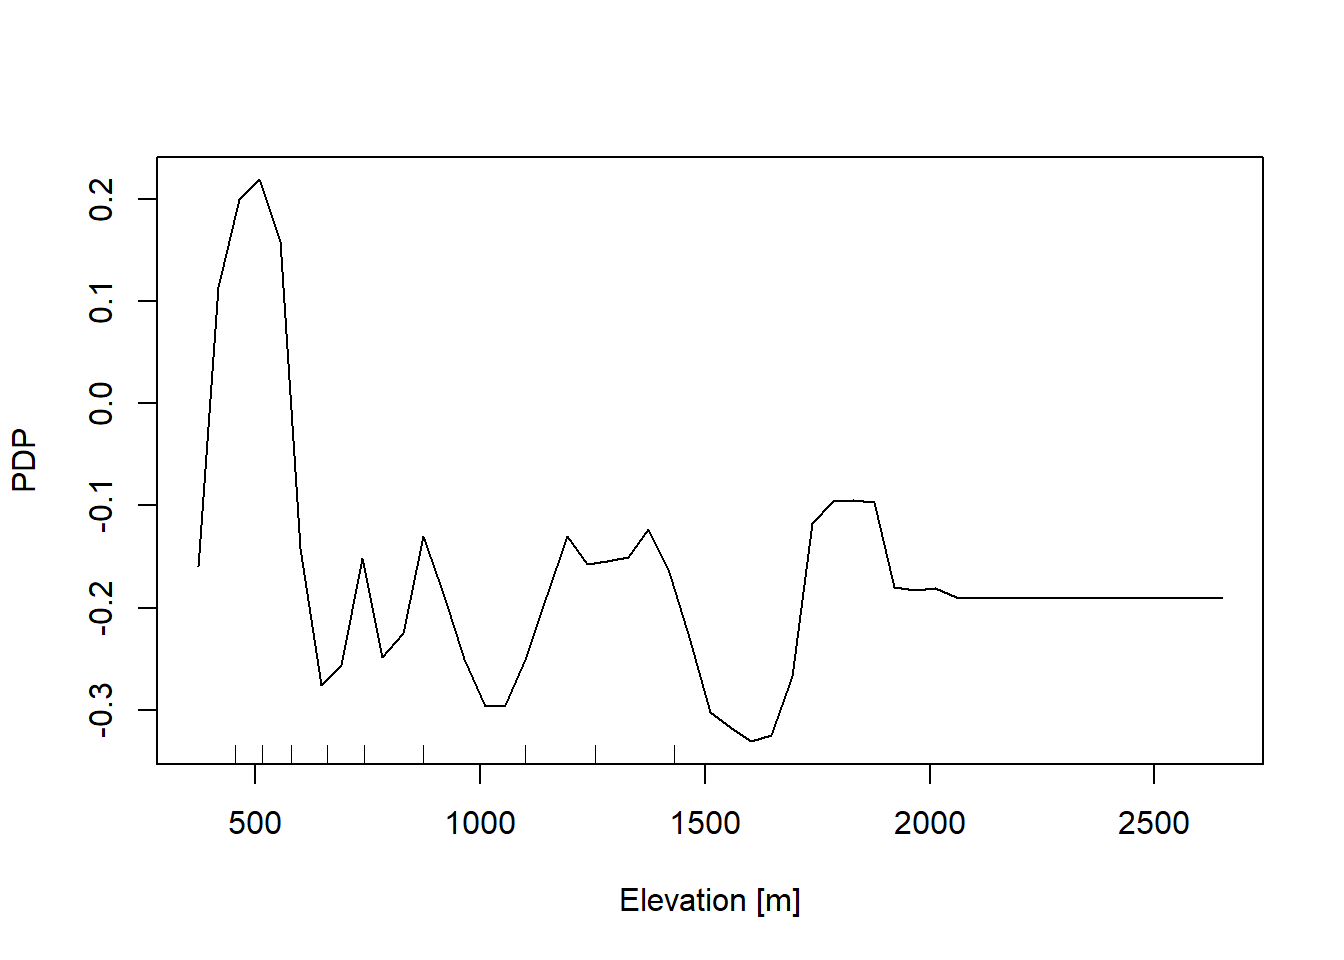
\includegraphics{06-Exp_RF_files/figure-latex/par-plot-2} \end{center}

\begin{Shaded}
\begin{Highlighting}[]
\CommentTok{\# Profile curvature}
\FunctionTok{partialPlot}\NormalTok{(RF\_LS, LS\_train, }\AttributeTok{x.var =}\NormalTok{ profCurv, }\AttributeTok{rug =} \ConstantTok{TRUE}\NormalTok{, }
            \AttributeTok{which.class =}\NormalTok{ RF\_LS}\SpecialCharTok{$}\NormalTok{classes[}\DecValTok{2}\NormalTok{],}\AttributeTok{xlab=} \StringTok{"Profile curvature [1/m]"}\NormalTok{, }
            \AttributeTok{main =} \StringTok{""}\NormalTok{, }\AttributeTok{ylab =} \StringTok{"PDP"}\NormalTok{, }\AttributeTok{xlim =} \FunctionTok{c}\NormalTok{(}\SpecialCharTok{{-}}\FloatTok{0.1}\NormalTok{,}\FloatTok{0.1}\NormalTok{))}
\end{Highlighting}
\end{Shaded}

\begin{center}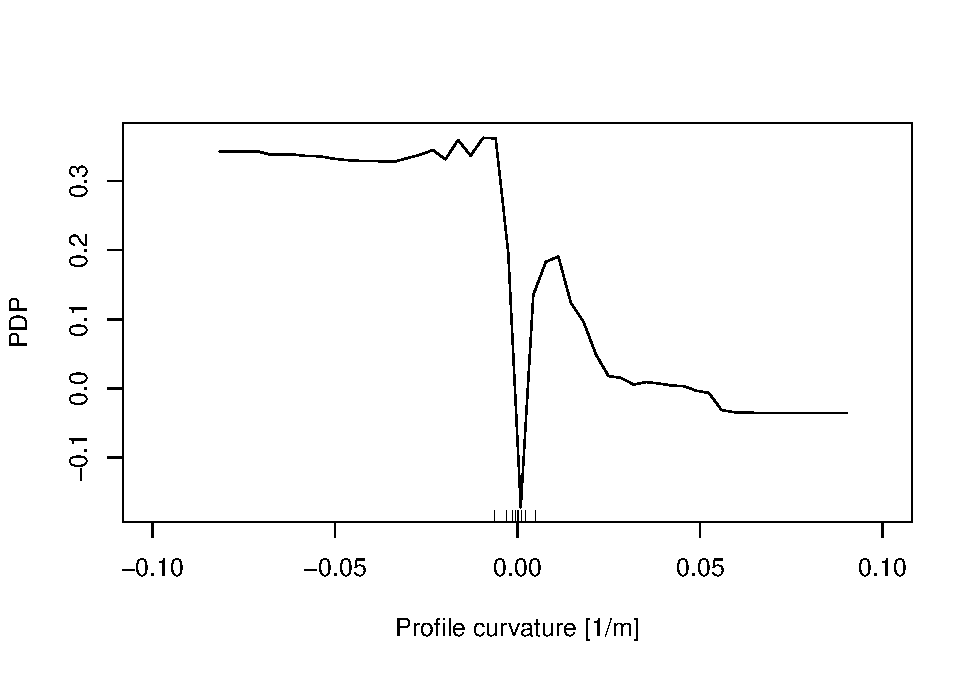
\includegraphics{06-Exp_RF_files/figure-latex/par-plot-3} \end{center}

\begin{Shaded}
\begin{Highlighting}[]
\CommentTok{\# Plan Curvature}
\FunctionTok{partialPlot}\NormalTok{(RF\_LS, LS\_train, }\AttributeTok{x.var =}\NormalTok{ planCurv, }\AttributeTok{rug =} \ConstantTok{TRUE}\NormalTok{, }
            \AttributeTok{which.class =}\NormalTok{ RF\_LS}\SpecialCharTok{$}\NormalTok{classes[}\DecValTok{2}\NormalTok{],}\AttributeTok{xlab=} \StringTok{"Plan curvature [1/m]"}\NormalTok{, }
            \AttributeTok{main =} \StringTok{""}\NormalTok{, }\AttributeTok{ylab =} \StringTok{"PDP"}\NormalTok{, }\AttributeTok{xlim =} \FunctionTok{c}\NormalTok{(}\SpecialCharTok{{-}}\FloatTok{0.1}\NormalTok{,}\FloatTok{0.1}\NormalTok{))}
\end{Highlighting}
\end{Shaded}

\begin{center}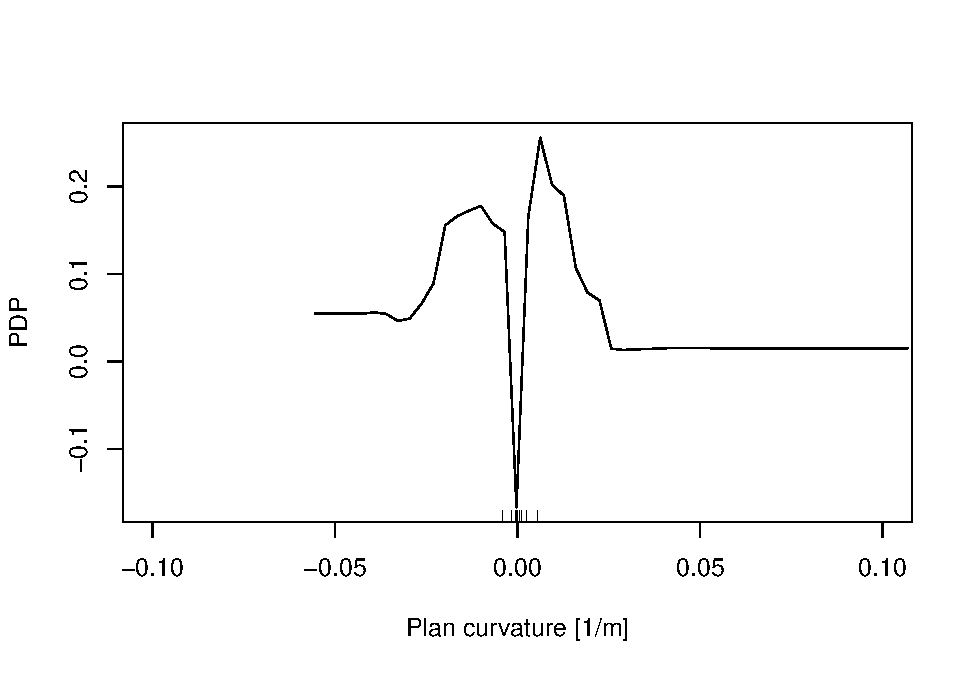
\includegraphics{06-Exp_RF_files/figure-latex/par-plot-4} \end{center}

\begin{Shaded}
\begin{Highlighting}[]
\CommentTok{\# Distance to road}
\FunctionTok{partialPlot}\NormalTok{(RF\_LS, LS\_train, }\AttributeTok{x.var =}\NormalTok{ distRoad, }\AttributeTok{rug =} \ConstantTok{TRUE}\NormalTok{, }
            \AttributeTok{which.class =}\NormalTok{ RF\_LS}\SpecialCharTok{$}\NormalTok{classes[}\DecValTok{2}\NormalTok{],}\AttributeTok{xlab=} \StringTok{"Distance to road [m]"}\NormalTok{, }
            \AttributeTok{main =} \StringTok{""}\NormalTok{, }\AttributeTok{ylab =} \StringTok{"PDP"}\NormalTok{)}
\end{Highlighting}
\end{Shaded}

\begin{center}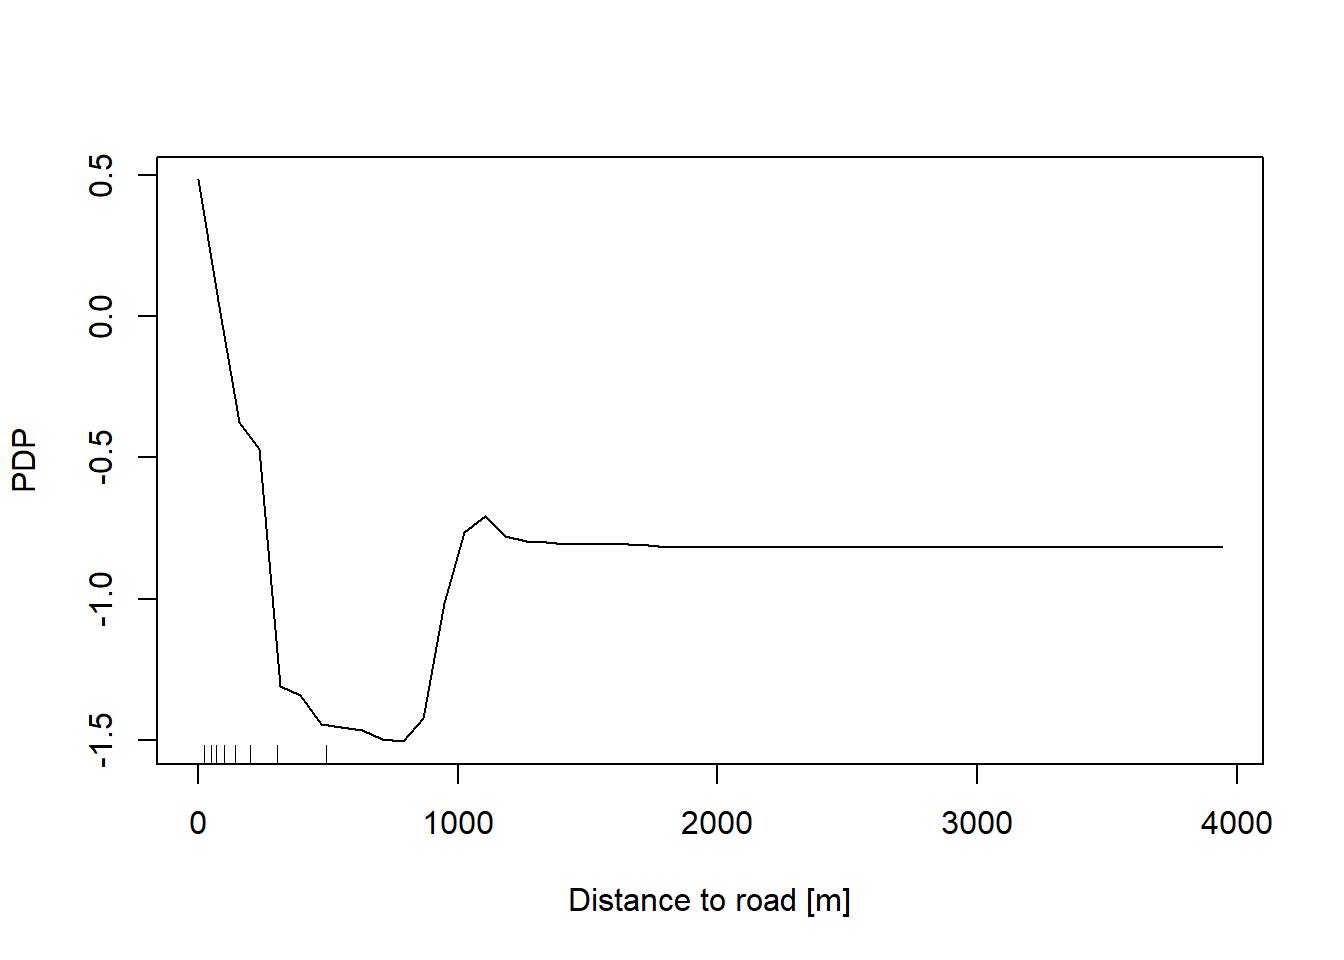
\includegraphics{06-Exp_RF_files/figure-latex/par-plot-5} \end{center}

\begin{Shaded}
\begin{Highlighting}[]
\CommentTok{\# Topographic wetness index}
\FunctionTok{partialPlot}\NormalTok{(RF\_LS, LS\_train, }\AttributeTok{x.var =}\NormalTok{ TWI, }\AttributeTok{rug =} \ConstantTok{TRUE}\NormalTok{, }
            \AttributeTok{which.class =}\NormalTok{ RF\_LS}\SpecialCharTok{$}\NormalTok{classes[}\DecValTok{2}\NormalTok{],}\AttributeTok{xlab=} \StringTok{"TWI [{-}]"}\NormalTok{, }
            \AttributeTok{main =} \StringTok{""}\NormalTok{, }\AttributeTok{ylab =} \StringTok{"PDP"}\NormalTok{)}
\end{Highlighting}
\end{Shaded}

\begin{center}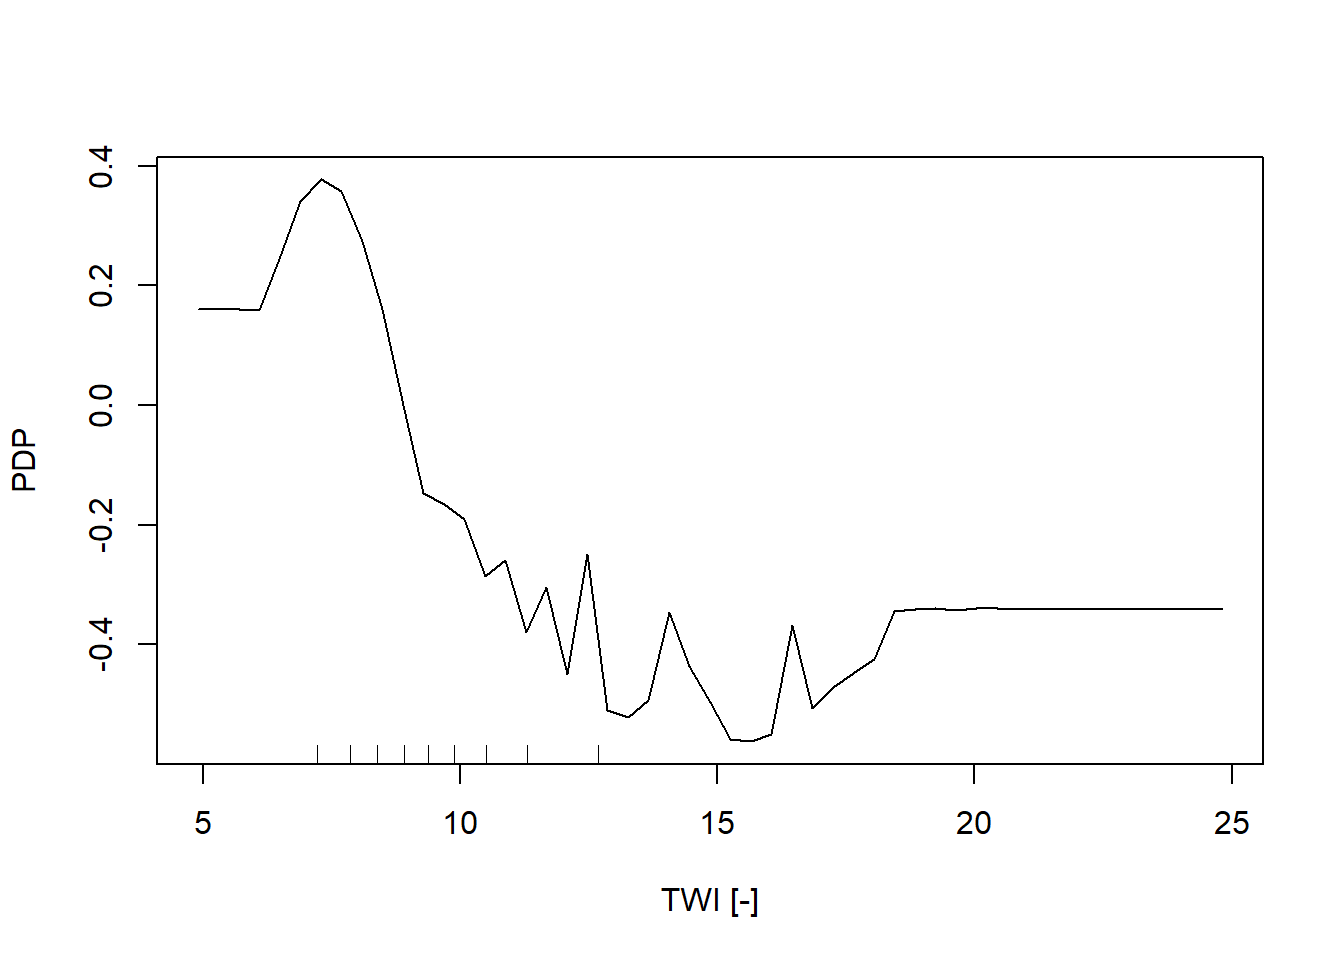
\includegraphics{06-Exp_RF_files/figure-latex/par-plot-6} \end{center}

\begin{Shaded}
\begin{Highlighting}[]
\CommentTok{\# Geology}
\FunctionTok{partialPlot}\NormalTok{(RF\_LS, LS\_train, }\AttributeTok{x.var =}\NormalTok{ geology, }\AttributeTok{rug =} \ConstantTok{TRUE}\NormalTok{, }
            \AttributeTok{which.class =}\NormalTok{ RF\_LS}\SpecialCharTok{$}\NormalTok{classes[}\DecValTok{2}\NormalTok{],}\AttributeTok{xlab=} \StringTok{"Geology"}\NormalTok{, }
            \AttributeTok{main =} \StringTok{""}\NormalTok{, }\AttributeTok{ylab =} \StringTok{"PDP"}\NormalTok{)}
\end{Highlighting}
\end{Shaded}

\begin{center}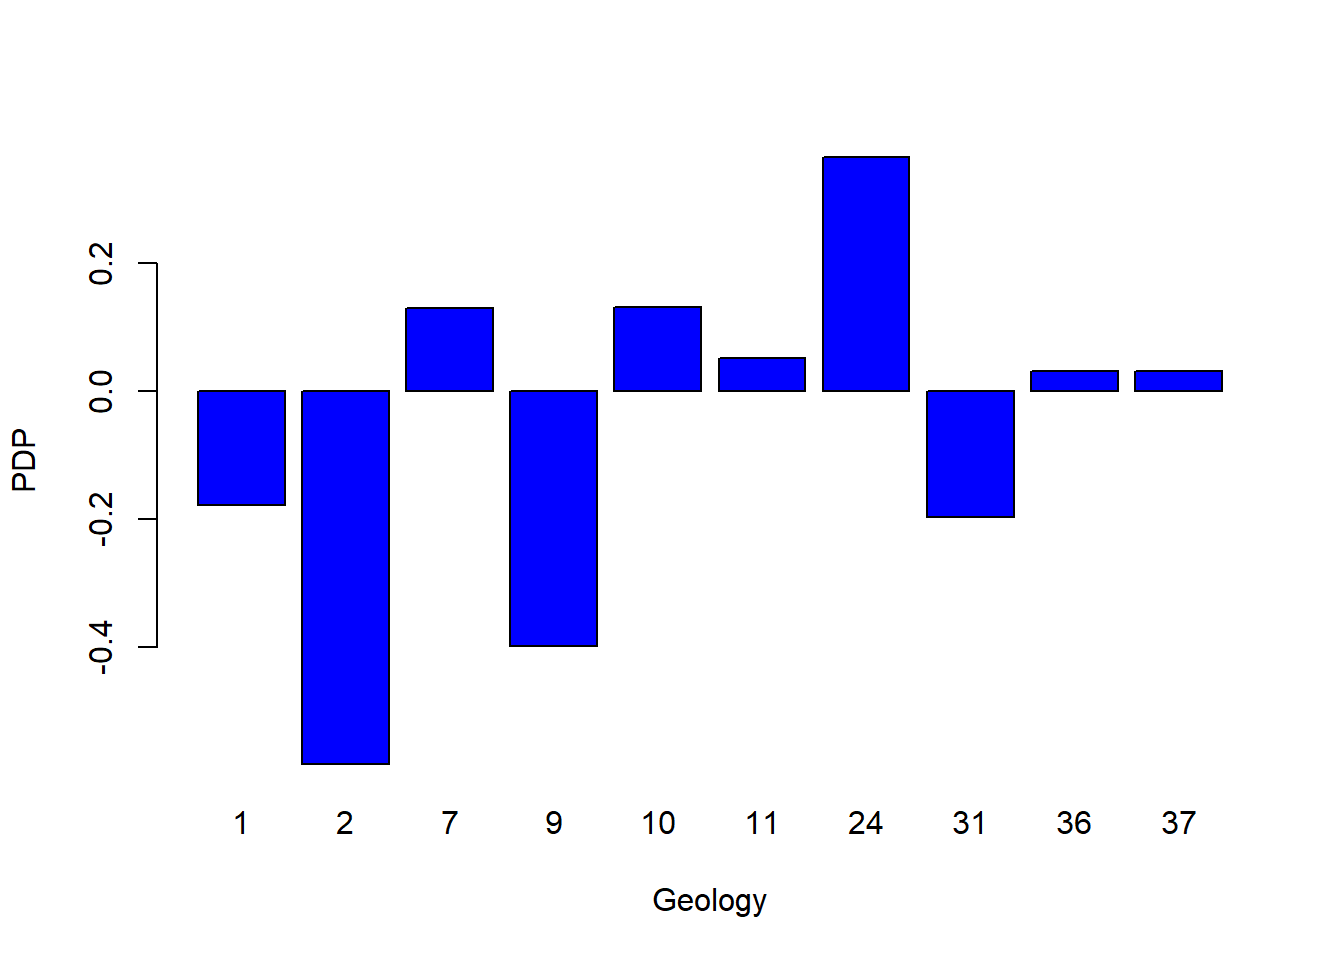
\includegraphics{06-Exp_RF_files/figure-latex/par-plot-7} \end{center}

\begin{Shaded}
\begin{Highlighting}[]
\CommentTok{\# Land cover}
\FunctionTok{partialPlot}\NormalTok{(RF\_LS, LS\_train, }\AttributeTok{x.var =}\NormalTok{ landCover, }\AttributeTok{rug =} \ConstantTok{TRUE}\NormalTok{, }
            \AttributeTok{which.class =}\NormalTok{ RF\_LS}\SpecialCharTok{$}\NormalTok{classes[}\DecValTok{2}\NormalTok{],}\AttributeTok{xlab=} \StringTok{"Land Cover"}\NormalTok{,}
            \AttributeTok{main =} \StringTok{""}\NormalTok{, }\AttributeTok{ylab =} \StringTok{"PDP"}\NormalTok{)}
\end{Highlighting}
\end{Shaded}

\begin{center}\includegraphics{06-Exp_RF_files/figure-latex/par-plot-8} \end{center}

\subsection{Local feature importance}\label{local-feature-importance}

Classical machine learning algorithms like Random Forest lack spatial calibration, hindering capturing the spatial heterogeneity in the relationship between a dependent and a set of independent variables.
To account for spatial heterogeneity (i.e.~non-stationarity) on the spatial patterns distribution of hazardous events modeled as function of geographical features we can use local models.
Specifically, in the present work we explore the \textbf{local feature importance} of geographical independent predictor variables on the spatial distribution of landslides in canton Vaud (Switzerland).

We introduce \textbf{Geographical Random Forest} (GRF), a spatial analysis method which uses a local version of RF algorithm \citep{georganos_forest_2022} .
This is achieved by fitting a sub-model for each observation in space, taking into account the neighboring observations.
The GRF can model the non-stationarity coupled with a non-linear model (RF), which, compared to liner models, tends not to overfit due to its bootstrapping nature.
In addition RF is suited for datasets with numerous predictor variables.

Essentially, GRF was designed to be a bridge between machine learning and geographical models, combining inferential and explanatory power.

\subsection{Computing lab: Geographical Random Forest}\label{computing-lab-geographical-random-forest}

For the computation we introduce here the method proposed by \citet{Georganos_forest_2022} and implemented in the R package \texttt{SpatialML} \citep{SpatialML}

The function \texttt{grf} fitting a local version of the RF algorithm, has been implemented fro regression problem, so we need to transform our binary response variable (presence==1 / absence==0) to a numeric value which can assume a range of values from zero to one.

\begin{verbatim}
## 'data.frame':    5173 obs. of  11 variables:
##  $ distRoad : num  176.8 70.7 35.4 35.4 90.1 ...
##  $ DEM      : num  442 450 453 453 462 ...
##  $ landCover: Factor w/ 7 levels "11","15","21",..: 3 1 1 1 3 1 3 3 3 3 ...
##  $ TWI      : num  8.28 8.11 8.3 8.3 8.58 ...
##  $ planCurv : num  0.000814 -0.005182 -0.001086 -0.001086 -0.000253 ...
##  $ profCurv : num  0.01217 0.0041 -0.00189 -0.00189 -0.00121 ...
##  $ slope    : num  17.6 5.38 8.8 8.8 3.36 ...
##  $ geology  : Factor w/ 10 levels "1","2","7","9",..: 7 7 7 7 7 7 7 7 7 7 ...
##  $ x        : num  567850 568050 567950 567950 567850 ...
##  $ y        : num  2e+05 2e+05 2e+05 2e+05 2e+05 ...
##  $ LS       : Factor w/ 2 levels "0","1": 2 2 2 2 2 2 2 2 2 2 ...
##  - attr(*, "na.action")= 'omit' Named int [1:15] 2598 2771 2939 2985 3237 3409 3456 3615 4058 4216 ...
##   ..- attr(*, "names")= chr [1:15] "2598" "2771" "2939" "2985" ...
\end{verbatim}

\begin{verbatim}
## 'data.frame':    4138 obs. of  12 variables:
##  $ distRoad : num  25 35.4 50 0 50 ...
##  $ DEM      : num  566 549 1151 1058 579 ...
##  $ landCover: Factor w/ 7 levels "11","15","21",..: 4 2 3 5 2 3 5 2 5 5 ...
##  $ TWI      : num  8.09 8.42 9.45 16.44 8.83 ...
##  $ planCurv : num  0.017138 0.001319 0.000871 -0.009321 -0.001597 ...
##  $ profCurv : num  -1.12e-02 3.92e-05 -3.13e-03 1.52e-02 4.64e-03 ...
##  $ slope    : num  5.49 15.33 13.87 5.05 10.35 ...
##  $ geology  : Factor w/ 10 levels "1","2","7","9",..: 1 1 1 2 1 1 1 1 5 1 ...
##  $ x        : num  558650 536550 560850 515450 535550 ...
##  $ y        : num  145400 154500 148400 168900 156800 ...
##  $ LS       : Factor w/ 2 levels "0","1": 2 2 2 1 1 2 1 2 1 2 ...
##  $ LSregr   : num  1 1 1 0 0 1 0 1 0 1 ...
##  - attr(*, "na.action")= 'omit' Named int [1:15] 2598 2771 2939 2985 3237 3409 3456 3615 4058 4216 ...
##   ..- attr(*, "names")= chr [1:15] "2598" "2771" "2939" "2985" ...
\end{verbatim}

\begin{verbatim}
## 'data.frame':    1035 obs. of  12 variables:
##  $ distRoad : num  79.1 111.8 35.4 35.4 25 ...
##  $ DEM      : num  484 1060 847 556 1327 ...
##  $ landCover: Factor w/ 7 levels "11","15","21",..: 3 5 2 3 3 3 2 5 1 3 ...
##  $ TWI      : num  10.9 11.2 10.1 10.5 10.2 ...
##  $ planCurv : num  -0.002085 -0.000343 -0.000788 0.000117 -0.001574 ...
##  $ profCurv : num  -0.001125 0.000457 0.001293 -0.000683 -0.002214 ...
##  $ slope    : num  14.39 1.97 15.91 4.74 20.62 ...
##  $ geology  : Factor w/ 10 levels "1","2","7","9",..: 7 1 7 1 1 1 1 2 7 1 ...
##  $ x        : num  529950 518550 552950 543550 572150 ...
##  $ y        : num  160700 165100 148200 174100 136000 ...
##  $ LS       : Factor w/ 2 levels "0","1": 2 1 2 1 2 1 2 1 2 1 ...
##  $ LSregr   : num  1 0 1 0 1 0 1 0 1 0 ...
##  - attr(*, "na.action")= 'omit' Named int [1:15] 2598 2771 2939 2985 3237 3409 3456 3615 4058 4216 ...
##   ..- attr(*, "names")= chr [1:15] "2598" "2771" "2939" "2985" ...
\end{verbatim}

\begin{Shaded}
\begin{Highlighting}[]
\NormalTok{Coords}\OtherTok{\textless{}{-}}\NormalTok{LS\_train[,}\DecValTok{9}\SpecialCharTok{:}\DecValTok{10}\NormalTok{] }\CommentTok{\# define coordinates}

\CommentTok{\# Run GRF}

\FunctionTok{set.seed}\NormalTok{(}\DecValTok{123}\NormalTok{) }\CommentTok{\# initialize }

\NormalTok{gwRF\_LS}\OtherTok{\textless{}{-}}\FunctionTok{grf}\NormalTok{(LSregr}\SpecialCharTok{\textasciitilde{}}\NormalTok{distRoad}\SpecialCharTok{+}\NormalTok{DEM}\SpecialCharTok{+}\NormalTok{landCover}\SpecialCharTok{+}\NormalTok{TWI}\SpecialCharTok{+}\NormalTok{planCurv}\SpecialCharTok{+}\NormalTok{profCurv}\SpecialCharTok{+}\NormalTok{slope}\SpecialCharTok{+}\NormalTok{geology,  LS\_train, }\AttributeTok{bw=}\DecValTok{40}\NormalTok{, }\AttributeTok{mtry=}\DecValTok{3}\NormalTok{, }\AttributeTok{kernel=}\StringTok{"adaptive"}\NormalTok{,}\AttributeTok{coords=}\NormalTok{Coords)}
\end{Highlighting}
\end{Shaded}

\begin{verbatim}
## Ranger result
## 
## Call:
##  ranger(LSregr ~ distRoad + DEM + landCover + TWI + planCurv +      profCurv + slope + geology, data = LS_train, num.trees = 500,      mtry = 3, importance = "impurity", num.threads = NULL) 
## 
## Type:                             Regression 
## Number of trees:                  500 
## Sample size:                      4138 
## Number of independent variables:  8 
## Mtry:                             3 
## Target node size:                 5 
## Variable importance mode:         impurity 
## Splitrule:                        variance 
## OOB prediction error (MSE):       0.1179855 
## R squared (OOB):                  0.5281665 
##  distRoad       DEM landCover       TWI  planCurv  profCurv     slope   geology 
## 189.03796 118.23180  42.58344 112.62676  86.64094 103.52100 275.56255  45.92905 
##     Min.  1st Qu.   Median     Mean  3rd Qu.     Max. 
## -1.00000 -0.03989  0.00000 -0.02352  0.01996  1.00000 
##       Min.    1st Qu.     Median       Mean    3rd Qu.       Max. 
## -0.5771719 -0.0038917  0.0000000 -0.0004654  0.0030000  0.4914078 
##           Min      Max      Mean       StD
## distRoad    0 5.057082 0.6840634 0.8651427
## DEM         0 5.097790 0.8308835 0.8286699
## landCover   0 3.263085 0.2288518 0.3818137
## TWI         0 4.108891 0.6034478 0.6340272
## planCurv    0 3.295054 0.4977787 0.4819980
## profCurv    0 4.177866 0.4866789 0.5209168
## slope       0 4.749768 0.8323274 0.8537186
## geology     0 4.923056 0.2181370 0.3916300
\end{verbatim}

\begin{Shaded}
\begin{Highlighting}[]
\FunctionTok{saveRDS}\NormalTok{(gwRF\_LS, }\StringTok{"gwRF\_LS.rds"}\NormalTok{)}
\end{Highlighting}
\end{Shaded}

\subsubsection{Global variable importance plot}\label{global-variable-importance-plot}

Based on the results of the GRF, we can plot of the variable importance ranking for illustrative purposes.
Values came from ``\texttt{Global\ ML\ Model\ Summary}'' --\textgreater{} ``\texttt{Importance}''

\begin{Shaded}
\begin{Highlighting}[]
\CommentTok{\# Create a data frame with variable names and importance values}
\NormalTok{variable\_importance }\OtherTok{\textless{}{-}} \FunctionTok{data.frame}\NormalTok{ (}
  \AttributeTok{Variable =} \FunctionTok{c}\NormalTok{(}\StringTok{"distRoad"}\NormalTok{, }\StringTok{"DEM"}\NormalTok{, }\StringTok{"landCover"}\NormalTok{, }\StringTok{"TWI"}\NormalTok{, }\StringTok{"planCurv"}\NormalTok{, }\StringTok{"profCurv"}\NormalTok{, }\StringTok{"slope"}\NormalTok{, }\StringTok{"geology"}\NormalTok{),}
  \AttributeTok{Importance =} \FunctionTok{c}\NormalTok{(}\FloatTok{181.18490}\NormalTok{, }\FloatTok{114.32444}\NormalTok{,  }\FloatTok{34.23643}\NormalTok{, }\FloatTok{101.51863}\NormalTok{,  }\FloatTok{84.81667}\NormalTok{, }\FloatTok{125.93651}\NormalTok{, }\FloatTok{297.74411}\NormalTok{,  }\FloatTok{39.22721}\NormalTok{ ) }\CommentTok{\# Importance {-} Global ML}
\NormalTok{)}

\CommentTok{\# Assign different colors to the top three important variables}
\NormalTok{variable\_importance}\SpecialCharTok{$}\NormalTok{Color }\OtherTok{\textless{}{-}} \FunctionTok{ifelse}\NormalTok{(variable\_importance}\SpecialCharTok{$}\NormalTok{Importance }\SpecialCharTok{\textgreater{}=} \FunctionTok{sort}\NormalTok{(variable\_importance}\SpecialCharTok{$}\NormalTok{Importance, }\AttributeTok{decreasing =} \ConstantTok{TRUE}\NormalTok{)[}\DecValTok{3}\NormalTok{], }\StringTok{"orange"}\NormalTok{, }\StringTok{"skyblue"}\NormalTok{)}

\CommentTok{\# Create a bar plot for variable importance with different colors for the top three variables}
\FunctionTok{ggplot}\NormalTok{(}\AttributeTok{data =}\NormalTok{ variable\_importance, }\FunctionTok{aes}\NormalTok{(}\AttributeTok{x =}\NormalTok{ Variable, }\AttributeTok{y =}\NormalTok{ Importance, }\AttributeTok{fill =}\NormalTok{ Color)) }\SpecialCharTok{+}
  \FunctionTok{geom\_bar}\NormalTok{(}\AttributeTok{stat =} \StringTok{"identity"}\NormalTok{) }\SpecialCharTok{+}
  \FunctionTok{scale\_fill\_identity}\NormalTok{() }\SpecialCharTok{+}
  \FunctionTok{labs}\NormalTok{(}\AttributeTok{title =} \StringTok{"Variable Importance Plot"}\NormalTok{, }\AttributeTok{x =} \StringTok{"Variable"}\NormalTok{, }\AttributeTok{y =} \StringTok{"Importance"}\NormalTok{) }\SpecialCharTok{+}
  \FunctionTok{theme}\NormalTok{(}\AttributeTok{axis.text.x =} \FunctionTok{element\_text}\NormalTok{(}\AttributeTok{angle =} \DecValTok{45}\NormalTok{, }\AttributeTok{hjust =} \DecValTok{1}\NormalTok{))  }\CommentTok{\# Rotate x{-}axis labels for better readability}
\end{Highlighting}
\end{Shaded}

\begin{center}\includegraphics{06-Exp_RF_files/figure-latex/Global-Var-Imp-1} \end{center}

\subsubsection{Local feature importance mapping}\label{local-feature-importance-mapping}

We can display the local feature importance scores for the two variables that are globally most important, the slope and the distance to road, with the output values mapped over the geographic space.

\begin{Shaded}
\begin{Highlighting}[]
\CommentTok{\# Create a data frame with the values of the local variables importance and the coordinates for each location}
\NormalTok{gwRF\_LS\_var}\OtherTok{\textless{}{-}}\NormalTok{gwRF\_LS}\SpecialCharTok{$}\NormalTok{Local.Variable.Importance}
\NormalTok{gwRF\_LS\_var\_XY}\OtherTok{\textless{}{-}}\FunctionTok{cbind}\NormalTok{(gwRF\_LS\_var,LS\_train}\SpecialCharTok{$}\NormalTok{x,LS\_train}\SpecialCharTok{$}\NormalTok{y ) }\CommentTok{\# add coordinates}
\FunctionTok{colnames}\NormalTok{(gwRF\_LS\_var\_XY)[}\DecValTok{9}\NormalTok{]}\OtherTok{\textless{}{-}} \StringTok{"X"} \CommentTok{\#rename column X{-}coordinate }
\FunctionTok{colnames}\NormalTok{(gwRF\_LS\_var\_XY)[}\DecValTok{10}\NormalTok{]}\OtherTok{\textless{}{-}} \StringTok{"Y"} \CommentTok{\#rename column Y{-}coordinate }
\FunctionTok{str}\NormalTok{(gwRF\_LS\_var\_XY) }
\end{Highlighting}
\end{Shaded}

\begin{verbatim}
## 'data.frame':    4138 obs. of  10 variables:
##  $ distRoad : num  0.0562 0.271 0.383 0.0165 0.2723 ...
##  $ DEM      : num  0.0427 0.8705 0.9203 0.5591 2.3373 ...
##  $ landCover: num  0.22036 0.04229 0.08014 0.00167 0.43775 ...
##  $ TWI      : num  0.1152 0.6513 0.4731 0.0766 1.3823 ...
##  $ planCurv : num  0.00755 0.59866 1.06332 0.03534 0.66228 ...
##  $ profCurv : num  0.0725 0.2454 0.8325 0.2023 0.8722 ...
##  $ slope    : num  0.00984 1.67939 1.23443 0.02137 1.13352 ...
##  $ geology  : num  0.0107 0.2399 0.3959 0.3438 1.8822 ...
##  $ X        : num  558650 536550 560850 515450 535550 ...
##  $ Y        : num  145400 154500 148400 168900 156800 ...
\end{verbatim}

\begin{Shaded}
\begin{Highlighting}[]
\FunctionTok{library}\NormalTok{(sf) }\CommentTok{\#for spatial data operations}
\CommentTok{\# Convert vector to sf (simple feature)}
\NormalTok{Vaud}\OtherTok{\textless{}{-}}\FunctionTok{vect}\NormalTok{(}\StringTok{"data/RF/Vaud\_CH.shp"}\NormalTok{)}
\NormalTok{Vaud\_sf}\OtherTok{\textless{}{-}}\FunctionTok{st\_as\_sf}\NormalTok{(Vaud) }

\CommentTok{\# Output predicted values are transformed to a vector}
\NormalTok{pred.vect }\OtherTok{\textless{}{-}} \FunctionTok{as.vector}\NormalTok{(gwRF\_LS\_var\_XY}\SpecialCharTok{$}\NormalTok{slope)}

\FunctionTok{library}\NormalTok{(classInt) }\CommentTok{\#for classification}

\NormalTok{brk}\OtherTok{\textless{}{-}}\NormalTok{(}\FunctionTok{classIntervals}\NormalTok{(pred.vect, }\AttributeTok{n=}\DecValTok{5}\NormalTok{, }\AttributeTok{style =} \StringTok{"fisher"}\NormalTok{))}
\NormalTok{brkInt}\OtherTok{\textless{}{-}}\FunctionTok{round}\NormalTok{(brk}\SpecialCharTok{$}\NormalTok{brks, }\AttributeTok{digits=}\DecValTok{2}\NormalTok{)}
\FunctionTok{print}\NormalTok{(brkInt)}
\end{Highlighting}
\end{Shaded}

\begin{verbatim}
## [1] 0.00 0.41 0.99 1.61 2.47 4.75
\end{verbatim}

\begin{Shaded}
\begin{Highlighting}[]
\CommentTok{\#natural breaks (fisher)}

\FunctionTok{ggplot}\NormalTok{() }\SpecialCharTok{+}
    \FunctionTok{geom\_point}\NormalTok{(}\AttributeTok{data =}\NormalTok{ gwRF\_LS\_var\_XY, }\FunctionTok{aes}\NormalTok{(}\AttributeTok{x =}\NormalTok{ X, }\AttributeTok{y =}\NormalTok{ Y, }\AttributeTok{colour =}\NormalTok{ slope), }\AttributeTok{size =} \DecValTok{1}\NormalTok{) }\SpecialCharTok{+}
    \FunctionTok{scale\_color\_gradientn}\NormalTok{(}\AttributeTok{colors =} \FunctionTok{c}\NormalTok{(}\StringTok{"white"}\NormalTok{, }\StringTok{"orange"}\NormalTok{,}\StringTok{"red"}\NormalTok{, }\StringTok{"blue"}\NormalTok{),  }
                       \AttributeTok{breaks =} \FunctionTok{c}\NormalTok{(}\FloatTok{0.00}\NormalTok{, }\FloatTok{0.40}\NormalTok{, }\FloatTok{1.15}\NormalTok{, }\FloatTok{2.11}\NormalTok{, }\FloatTok{3.23}\NormalTok{, }\FloatTok{4.91}\NormalTok{), }
                       \AttributeTok{labels=}\FunctionTok{c}\NormalTok{(}\FloatTok{0.00}\NormalTok{, }\FloatTok{0.40}\NormalTok{, }\FloatTok{1.15}\NormalTok{, }\FloatTok{2.11}\NormalTok{, }\FloatTok{3.23}\NormalTok{, }\FloatTok{4.91}\NormalTok{)) }\SpecialCharTok{+}
        \FunctionTok{labs}\NormalTok{( }\AttributeTok{x =} \StringTok{"X Coordinate"}\NormalTok{, }\AttributeTok{y =} \StringTok{"Y Coordinate"}\NormalTok{)}\SpecialCharTok{+}
    \FunctionTok{ggtitle}\NormalTok{(}\StringTok{"Local average FI {-} Slope"}\NormalTok{)}\SpecialCharTok{+}
    \FunctionTok{geom\_sf}\NormalTok{(}\AttributeTok{data =}\NormalTok{ Vaud\_sf, }\AttributeTok{fill =} \StringTok{"transparent"}\NormalTok{, }\AttributeTok{color =} \StringTok{"black"}\NormalTok{, }\AttributeTok{size=}\DecValTok{2}\NormalTok{) }\CommentTok{\#overlap borders}
\end{Highlighting}
\end{Shaded}

\begin{center}\includegraphics{06-Exp_RF_files/figure-latex/Slope_Imp-1} \end{center}

\begin{Shaded}
\begin{Highlighting}[]
\CommentTok{\# Output predicted values are transformed to a vector}
\NormalTok{pred.vect }\OtherTok{\textless{}{-}} \FunctionTok{as.vector}\NormalTok{(gwRF\_LS}\SpecialCharTok{$}\NormalTok{Local.Variable.Importance}\SpecialCharTok{$}\NormalTok{distRoad)}
 
\NormalTok{brk}\OtherTok{\textless{}{-}}\NormalTok{(}\FunctionTok{classIntervals}\NormalTok{(pred.vect, }\AttributeTok{n=}\DecValTok{5}\NormalTok{, }\AttributeTok{style =} \StringTok{"fisher"}\NormalTok{))}
\NormalTok{brkInt}\OtherTok{\textless{}{-}}\FunctionTok{round}\NormalTok{(brk}\SpecialCharTok{$}\NormalTok{brks, }\AttributeTok{digits=}\DecValTok{2}\NormalTok{)}
\FunctionTok{print}\NormalTok{(brkInt) }\CommentTok{\# print breaks}
\end{Highlighting}
\end{Shaded}

\begin{verbatim}
## [1] 0.00 0.39 1.06 2.08 3.48 5.06
\end{verbatim}

\begin{Shaded}
\begin{Highlighting}[]
\CommentTok{\#natural breaks (fisher)}

\FunctionTok{ggplot}\NormalTok{() }\SpecialCharTok{+}
    \FunctionTok{geom\_point}\NormalTok{(}\AttributeTok{data =}\NormalTok{ gwRF\_LS\_var\_XY, }\FunctionTok{aes}\NormalTok{(}\AttributeTok{x =}\NormalTok{ X, }\AttributeTok{y =}\NormalTok{ Y, }\AttributeTok{colour =}\NormalTok{ distRoad), }\AttributeTok{size =} \DecValTok{1}\NormalTok{) }\SpecialCharTok{+}
    \FunctionTok{scale\_color\_gradientn}\NormalTok{(}\AttributeTok{colors =} \FunctionTok{c}\NormalTok{(}\StringTok{"white"}\NormalTok{, }\StringTok{"orange"}\NormalTok{,}\StringTok{"red"}\NormalTok{, }\StringTok{"blue"}\NormalTok{), }
                       \AttributeTok{breaks =} \FunctionTok{c}\NormalTok{(}\FloatTok{0.00}\NormalTok{, }\FloatTok{0.37}\NormalTok{, }\FloatTok{1.02}\NormalTok{, }\FloatTok{2.17}\NormalTok{, }\FloatTok{3.58}\NormalTok{, }\FloatTok{4.85}\NormalTok{), }
                       \AttributeTok{labels=}\FunctionTok{c}\NormalTok{(}\FloatTok{0.00}\NormalTok{, }\FloatTok{0.37}\NormalTok{, }\FloatTok{1.02}\NormalTok{, }\FloatTok{2.17}\NormalTok{, }\FloatTok{3.58}\NormalTok{, }\FloatTok{4.85}\NormalTok{)) }\SpecialCharTok{+}
    \FunctionTok{labs}\NormalTok{( }\AttributeTok{x =} \StringTok{"X Coordinate"}\NormalTok{, }\AttributeTok{y =} \StringTok{"Y Coordinate"}\NormalTok{)}\SpecialCharTok{+}
    \FunctionTok{ggtitle}\NormalTok{(}\StringTok{"Local average FI {-} Distance to roads"}\NormalTok{)}\SpecialCharTok{+}
    \FunctionTok{geom\_sf}\NormalTok{(}\AttributeTok{data =}\NormalTok{ Vaud\_sf, }\AttributeTok{fill =} \StringTok{"transparent"}\NormalTok{, }\AttributeTok{color =} \StringTok{"black"}\NormalTok{, }\AttributeTok{size=}\DecValTok{2}\NormalTok{) }\CommentTok{\#overlap borders}
\end{Highlighting}
\end{Shaded}

\begin{center}\includegraphics{06-Exp_RF_files/figure-latex/distRoad-Imp-1} \end{center}

\subsubsection{Local R squared}\label{local-r-squared}

The Local R-squared value represents the strength of the correlations of the local model on the predictor variables and ranges from 0 to 1.

\begin{Shaded}
\begin{Highlighting}[]
\NormalTok{Rsq}\OtherTok{\textless{}{-}}\NormalTok{gwRF\_LS}\SpecialCharTok{$}\NormalTok{LGofFit}\SpecialCharTok{$}\NormalTok{LM\_Rsq100}
\NormalTok{Rsq\_XY}\OtherTok{\textless{}{-}}\FunctionTok{as.data.frame}\NormalTok{(}\FunctionTok{cbind}\NormalTok{(Rsq,LS\_train}\SpecialCharTok{$}\NormalTok{x,LS\_train}\SpecialCharTok{$}\NormalTok{y)) }\CommentTok{\# add coordinates}
\FunctionTok{colnames}\NormalTok{(Rsq\_XY)[}\DecValTok{2}\NormalTok{]}\OtherTok{\textless{}{-}} \StringTok{"X"}
\FunctionTok{colnames}\NormalTok{(Rsq\_XY)[}\DecValTok{3}\NormalTok{]}\OtherTok{\textless{}{-}} \StringTok{"Y"}
\FunctionTok{str}\NormalTok{(Rsq\_XY)}
\end{Highlighting}
\end{Shaded}

\begin{verbatim}
## 'data.frame':    4138 obs. of  3 variables:
##  $ Rsq: num  -0.258 0.537 -0.144 -0.255 0.322 ...
##  $ X  : num  558650 536550 560850 515450 535550 ...
##  $ Y  : num  145400 154500 148400 168900 156800 ...
\end{verbatim}

\begin{Shaded}
\begin{Highlighting}[]
\FunctionTok{ggplot}\NormalTok{ () }\SpecialCharTok{+}
  \FunctionTok{geom\_point}\NormalTok{(}\AttributeTok{data =}\NormalTok{ Rsq\_XY, }\FunctionTok{aes}\NormalTok{(}\AttributeTok{x =}\NormalTok{ X, }\AttributeTok{y =}\NormalTok{ Y, }\AttributeTok{colour =}\NormalTok{ Rsq), }\AttributeTok{size =} \DecValTok{1}\NormalTok{)}\SpecialCharTok{+} 
  \FunctionTok{scale\_color\_gradientn}\NormalTok{(}\AttributeTok{colors =} \FunctionTok{c}\NormalTok{(}\StringTok{"white"}\NormalTok{, }\StringTok{"yellow"}\NormalTok{,}\StringTok{"red"}\NormalTok{, }\StringTok{"blue"}\NormalTok{))}\SpecialCharTok{+}
  \FunctionTok{labs}\NormalTok{(}\AttributeTok{title =} \StringTok{"Rsq"}\NormalTok{, }\AttributeTok{x =} \StringTok{"X Coordinate"}\NormalTok{, }\AttributeTok{y =} \StringTok{"Y Coordinate"}\NormalTok{)}\SpecialCharTok{+}
  \FunctionTok{ggtitle}\NormalTok{(}\StringTok{"Local R2"}\NormalTok{)}\SpecialCharTok{+}
  \FunctionTok{geom\_sf}\NormalTok{(}\AttributeTok{data =}\NormalTok{ Vaud\_sf, }\AttributeTok{fill =} \StringTok{"transparent"}\NormalTok{, }\AttributeTok{color =} \StringTok{"black"}\NormalTok{, }\AttributeTok{size=}\DecValTok{2}\NormalTok{) }\CommentTok{\#overlap borders}
\end{Highlighting}
\end{Shaded}

\begin{center}\includegraphics{06-Exp_RF_files/figure-latex/local-R2-1} \end{center}

\subsection{Conclusions and further analyses}\label{conclusions-and-further-analyses-3}

In the present exercise GRF has been used as a purely exploratory tool to estimate the spatial variation of the relationship between landslides in Canton Vaud (Switzerland) and the predictor variables.
It allowed to elaborate maps based on the local average importance of the most highly correlated features and to visualize the local fitting performance (R2 local value) into a map.

To ensure that everything is perfectly clear, we propose you to answer the following questions:

\begin{enumerate}
\def\labelenumi{\arabic{enumi}.}
\item
  Among the following algorithms evaluate them in therms of their interpretability and explainability: Support Vector Machines , linear regression, Deep Learning Models, Decision Trees, K-Nearest Neighbors, Neural Networks, Random Forests, logistic regression.
\item
  Which are the three most important variables of your model (based on the MDA)?
\item
  What is the slope value (or range of values) that gives the highest probability of landslides occurrence?
  And for the geology, which are the most important classes?
\item
  Evaluate the spatial variation of the relationship between landslides and slope / distance to roads in your study area by visually inspecting the local average importance of these features.
\item
  You can replicate this code (some chiuncks of it) to evaluate the local average importance of the third most important variable, as well as to map the local mean squared error.
\end{enumerate}

\section{Defining Territorial Typologies Using Unsupervised Learning: A SOM Approach}\label{som}

Urban expansion across Europe has accelerated in recent decades, significantly blurring the distinctions between urban and rural landscapes.
The growing complexity and constant evolution of territorial dynamics require timely urban-rural typologies that systematically classify areas along the continuum from distinctly urban to distinctly rural.
Traditional threshold-based classification methods rely heavily on expert input and are labor-intensive, hindering timely updates.
This study addresses the issue by developing an unsupervised learning approach based on \textbf{Self-Organizing Map (SOM)} \citep{kohonen_self-organized_1982} to group Swiss municipalities, using a diverse set of demographic, socioeconomic, and built environment variables.

\subsection{Geo-demographic context in Switzerland}\label{geo-demographic-context-in-switzerland}

Switzerland has the highest life expectancy in the world.
It counts about 8,5 million inhabitants (official census data 2020), twice as much as at the beginning of the 20th century, mainly because of the high level of immigration.
The number of foreigners that currently reside in the country corresponds to about one quarter of the total population.
Most of the population (85\%) lives in cities.
Population aging increased over the course of the 20th century, with one in five person of retirement age today.

\subsubsection{Swiss census data}\label{swiss-census-data}

The input census data used in this study come from the \href{https://www.bfs.admin.ch/bfs/en/home.html}{Swiss Federal Statistical Office} and have been downloaded from the Statistical Atlas of Switzerland \citep{FSO_2024}.
Following an in-depth analysis of all data available in the Atlas, eighteen variables from the 2020 census were selected.
These variables provide a comprehensive overview of the physical environment (including settlement, forest, agricultural, unproductive, and traffic areas), demographic characteristics (such as natural growth, population density, international and internal migration, proportion of foreigners, youth, and senior population), and the socio-economic profile (covering employment, new buildings, new houses, individual housing, new enterprises, and net income) of the resident population.
This information has been aggregated to the municipality level for the purpose of the present investigation.

\subsection{Self Organizing Map}\label{self-organizing-map}

We use SOM, an unsupervised competitive learning neural network allowing representing a high-dimensional feature space (defined by the multivariate input dataset), as two-dimensional discretized pattern (the SOM grid of neurons).
In SOM the proximity of the units in the output grid reflects the similarity of the corresponding input observations, which guarantees the preservation of the topological structure of the input data.

Compared to other approaches, SOM is very efficient for data visualization.
Indeed it provides additional outputs such as the heatmaps, representing the distribution of each input feature across the SOM grid, extremely useful to visually explore the relationship between the input variables.

\subsection{Computing lab: SOM}\label{computing-lab-som}

\subsubsection{Load the libraries}\label{load-the-libraries-3}

To perform the analyses and visualize the results you have to load the following libraries:

\begin{itemize}
\tightlist
\item
  \emph{kohonen}: Supervised and Unsupervised Self-Organizing Maps (SOM)
\item
  \emph{aweSOM}\textbf{:} offers a set of tools to explore and analyze datasets with SOM
\item
  \emph{ggplot2}: create Elegant Data Visualizations Using the Grammar of Graphics
\item
  \emph{colorpatch}: rendering methods (ggplot extensions)
\end{itemize}

\begin{Shaded}
\begin{Highlighting}[]
\FunctionTok{library}\NormalTok{(kohonen)}
\FunctionTok{library}\NormalTok{(aweSOM)}
\FunctionTok{library}\NormalTok{(ggplot2)}
\FunctionTok{library}\NormalTok{(colorpatch)}
\NormalTok{(}\FunctionTok{.packages}\NormalTok{())}
\end{Highlighting}
\end{Shaded}

\subsubsection{Import the Swiss census dataset}\label{import-the-swiss-census-dataset}

Fist, you have to import the Swiss census dataset for the year 2020, referred to the municipality administrative units.
As you can see from the description of the selected variables \autoref{Variables}, some of them can be discarded from the analysis.
So, in the following step, we extract a subset of the most meaningful variables for the purpose of the present study.

\begin{Shaded}
\begin{Highlighting}[]
\NormalTok{knitr}\SpecialCharTok{::}\FunctionTok{include\_graphics}\NormalTok{(}\FunctionTok{c}\NormalTok{(}\StringTok{"images/Variables1.jpg"}\NormalTok{, }\StringTok{"images/Variables2.jpg"}\NormalTok{))}
\end{Highlighting}
\end{Shaded}

\begin{figure}

{\centering \includegraphics[width=1\linewidth,height=1\textheight]{images/Variables1} 

}

\caption{Variables description \label{Variables}}\label{fig:variables-1}
\end{figure}
\begin{figure}

{\centering \includegraphics[width=1\linewidth,height=1\textheight]{images/Variables2} 

}

\caption{Variables description \label{Variables}}\label{fig:variables-2}
\end{figure}

\paragraph{Inspect the data}\label{inspect-the-data}

Histograms can be used to show the frequency distribution of the variables and help detect patterns, such as skewness, outliers, and the range of values. Similarly, box plots summarize data using quartiles, helping to identify central tendency, spread, and outliers. Together, these visual tools allow to asses if variables have comparable ranges and help determine if data transformation is needed.

\begin{Shaded}
\begin{Highlighting}[]
\CommentTok{\# Plot variables\textquotesingle{} frequency distribution}
\ControlFlowTok{for}\NormalTok{(i }\ControlFlowTok{in} \DecValTok{3}\SpecialCharTok{:}\FunctionTok{ncol}\NormalTok{(subset2020)) \{      }
    \FunctionTok{hist}\NormalTok{((subset2020[ , i]),  }\AttributeTok{main=}\FunctionTok{colnames}\NormalTok{(subset2020[i]))}
\NormalTok{\}}
\end{Highlighting}
\end{Shaded}

\begin{Shaded}
\begin{Highlighting}[]
\CommentTok{\# Plot variables\textquotesingle{} frequency distribution}
\ControlFlowTok{for}\NormalTok{(i }\ControlFlowTok{in} \DecValTok{3}\SpecialCharTok{:}\FunctionTok{ncol}\NormalTok{(subset2020)) \{      }
    \FunctionTok{boxplot}\NormalTok{((subset2020[ , i]),  }\AttributeTok{main=}\FunctionTok{colnames}\NormalTok{(subset2020[i]))}
\NormalTok{\}}
\end{Highlighting}
\end{Shaded}

\paragraph{Data transformation}\label{data-transformation}

To make the variables range comparable, we propose to operate the max-min normalization scaling input census data in the range {[}0 -- 1{]}. Computationally it subtracts the minimum value from the original one, and then it divides the result by the range (i.e., difference between the maximum and minimum values). This process ensures that all variables in the dataset are in the same range, and can be treated and evaluated together.

However, the min-max transformation is sensitive to outliers, as extreme values can distort the interpretation by compressing the range. To mitigate this, values beyond the upper and lower 5th percentiles will be capped at these thresholds before operating the max-min normalization.

\begin{Shaded}
\begin{Highlighting}[]
\CommentTok{\# Define the general function to detect outlier}
\NormalTok{replace\_outliers }\OtherTok{\textless{}{-}} \ControlFlowTok{function}\NormalTok{(df, lower\_quantile\_value, upper\_quantile\_value) \{}
\NormalTok{  replaced\_df }\OtherTok{\textless{}{-}}\NormalTok{ df}
  \ControlFlowTok{for}\NormalTok{ (col }\ControlFlowTok{in} \FunctionTok{names}\NormalTok{(df)) \{}
\NormalTok{    lower\_quantile }\OtherTok{\textless{}{-}} \FunctionTok{quantile}\NormalTok{(df[[col]], }\AttributeTok{probs =}\NormalTok{ lower\_quantile\_value)}
\NormalTok{    upper\_quantile }\OtherTok{\textless{}{-}} \FunctionTok{quantile}\NormalTok{(df[[col]], }\AttributeTok{probs =}\NormalTok{ upper\_quantile\_value)}
\NormalTok{    outlier\_indices\_lower }\OtherTok{\textless{}{-}}\NormalTok{ df[[col]] }\SpecialCharTok{\textless{}}\NormalTok{ lower\_quantile}
\NormalTok{    outlier\_indices\_upper }\OtherTok{\textless{}{-}}\NormalTok{ df[[col]] }\SpecialCharTok{\textgreater{}}\NormalTok{ upper\_quantile}
\NormalTok{    replaced\_df[[col]][outlier\_indices\_lower] }\OtherTok{\textless{}{-}}\NormalTok{ lower\_quantile}
\NormalTok{    replaced\_df[[col]][outlier\_indices\_upper] }\OtherTok{\textless{}{-}}\NormalTok{ upper\_quantile}
\NormalTok{  \}}
  \FunctionTok{return}\NormalTok{(replaced\_df)}
\NormalTok{\}}

\CommentTok{\# Define the percentile level}
\NormalTok{lower\_quantile\_value }\OtherTok{\textless{}{-}} \FloatTok{0.05}
\NormalTok{upper\_quantile\_value }\OtherTok{\textless{}{-}} \FloatTok{0.95}

\CommentTok{\# Replace outliers in all variables with upper and lower quantile values}

\NormalTok{df2020\_out\_repl }\OtherTok{\textless{}{-}} \FunctionTok{replace\_outliers}\NormalTok{((subset2020[ , }\SpecialCharTok{{-}}\FunctionTok{c}\NormalTok{(}\DecValTok{1}\NormalTok{,}\DecValTok{2}\NormalTok{)]), lower\_quantile\_value, upper\_quantile\_value)}
\FunctionTok{summary}\NormalTok{ (df2020\_out\_repl)}
\end{Highlighting}
\end{Shaded}

\begin{verbatim}
##  p_infrastructure    p_forested      p_agriculture    p_improductible   
##  Min.   :0.01906   Min.   :0.07797   Min.   :0.1030   Min.   :0.000000  
##  1st Qu.:0.06232   1st Qu.:0.20751   1st Qu.:0.3190   1st Qu.:0.003188  
##  Median :0.10815   Median :0.31211   Median :0.4694   Median :0.010854  
##  Mean   :0.15093   Mean   :0.32368   Mean   :0.4492   Mean   :0.056692  
##  3rd Qu.:0.20430   3rd Qu.:0.42620   3rd Qu.:0.5970   3rd Qu.:0.047372  
##  Max.   :0.48058   Max.   :0.61755   Max.   :0.7312   Max.   :0.402194  
##   p_transport      natural_growth       density        migration_intern 
##  Min.   : 0.7136   Min.   :-9.0172   Min.   :  16.42   Min.   :-24.648  
##  1st Qu.: 1.9811   1st Qu.:-2.1720   1st Qu.:  82.34   1st Qu.: -7.159  
##  Median : 3.2459   Median : 0.8865   Median : 189.46   Median :  2.575  
##  Mean   : 4.1497   Mean   : 0.7120   Mean   : 374.19   Mean   :  3.904  
##  3rd Qu.: 5.4475   3rd Qu.: 3.9575   3rd Qu.: 480.88   3rd Qu.: 13.534  
##  Max.   :11.9374   Max.   : 9.2336   Max.   :1662.06   Max.   : 37.746  
##    migration       p_foreigners    p_individual_houses    p_pop_19    
##  Min.   :-5.896   Min.   : 4.419   Min.   :32.94       Min.   :14.83  
##  1st Qu.: 0.000   1st Qu.: 9.736   1st Qu.:51.46       1st Qu.:18.61  
##  Median : 3.389   Median :15.432   Median :61.54       Median :20.53  
##  Mean   : 4.071   Mean   :16.915   Mean   :59.55       Mean   :20.44  
##  3rd Qu.: 7.250   3rd Qu.:23.487   3rd Qu.:68.93       3rd Qu.:22.38  
##  Max.   :17.350   Max.   :35.327   Max.   :78.69       Max.   :25.47  
##     p_pop_65      p_employment     p_new_buildings  p_new_housings   
##  Min.   :13.22   Min.   :0.07255   Min.   :0.0000   Min.   : 0.0000  
##  1st Qu.:16.60   1st Qu.:0.14204   1st Qu.:0.3201   1st Qu.: 0.5315  
##  Median :19.16   Median :0.22970   Median :1.2799   Median : 3.0057  
##  Mean   :19.51   Mean   :0.28020   Mean   :1.7691   Mean   : 5.0709  
##  3rd Qu.:21.95   3rd Qu.:0.36167   3rd Qu.:2.6316   3rd Qu.: 7.2601  
##  Max.   :27.60   Max.   :0.75642   Max.   :6.2107   Max.   :21.1283  
##  p_new_entreprise     net_income   
##  Min.   :0.000000   Min.   :25908  
##  1st Qu.:0.000000   1st Qu.:30789  
##  Median :0.002931   Median :34960  
##  Mean   :0.002806   Mean   :36848  
##  3rd Qu.:0.004514   3rd Qu.:40433  
##  Max.   :0.007919   Max.   :59032
\end{verbatim}

\begin{Shaded}
\begin{Highlighting}[]
\CommentTok{\# Define the general function for min{-}max normalization}
\NormalTok{minMax }\OtherTok{\textless{}{-}} \ControlFlowTok{function}\NormalTok{(x) \{}
\NormalTok{  (x }\SpecialCharTok{{-}} \FunctionTok{min}\NormalTok{(x)) }\SpecialCharTok{/}\NormalTok{ (}\FunctionTok{max}\NormalTok{(x) }\SpecialCharTok{{-}} \FunctionTok{min}\NormalTok{(x))}
\NormalTok{\}}

\CommentTok{\# Apply max{-}min to the data}
\NormalTok{dfnorm2020\_out\_repl}\OtherTok{\textless{}{-}} \FunctionTok{as.data.frame}\NormalTok{(}\FunctionTok{lapply}\NormalTok{((df2020\_out\_repl), minMax))}
\FunctionTok{summary}\NormalTok{(dfnorm2020\_out\_repl)}
\end{Highlighting}
\end{Shaded}

\begin{verbatim}
##  p_infrastructure    p_forested     p_agriculture    p_improductible   
##  Min.   :0.00000   Min.   :0.0000   Min.   :0.0000   Min.   :0.000000  
##  1st Qu.:0.09373   1st Qu.:0.2401   1st Qu.:0.3439   1st Qu.:0.007927  
##  Median :0.19304   Median :0.4339   Median :0.5833   Median :0.026987  
##  Mean   :0.28573   Mean   :0.4554   Mean   :0.5510   Mean   :0.140958  
##  3rd Qu.:0.40137   3rd Qu.:0.6454   3rd Qu.:0.7863   3rd Qu.:0.117785  
##  Max.   :1.00000   Max.   :1.0000   Max.   :1.0000   Max.   :1.000000  
##   p_transport     natural_growth      density        migration_intern
##  Min.   :0.0000   Min.   :0.0000   Min.   :0.00000   Min.   :0.0000  
##  1st Qu.:0.1129   1st Qu.:0.3751   1st Qu.:0.04005   1st Qu.:0.2803  
##  Median :0.2256   Median :0.5426   Median :0.10515   Median :0.4363  
##  Mean   :0.3061   Mean   :0.5331   Mean   :0.21740   Mean   :0.4576  
##  3rd Qu.:0.4218   3rd Qu.:0.7109   3rd Qu.:0.28224   3rd Qu.:0.6119  
##  Max.   :1.0000   Max.   :1.0000   Max.   :1.00000   Max.   :1.0000  
##    migration       p_foreigners    p_individual_houses    p_pop_19     
##  Min.   :0.0000   Min.   :0.0000   Min.   :0.0000      Min.   :0.0000  
##  1st Qu.:0.2536   1st Qu.:0.1720   1st Qu.:0.4048      1st Qu.:0.3560  
##  Median :0.3994   Median :0.3563   Median :0.6251      Median :0.5357  
##  Mean   :0.4288   Mean   :0.4043   Mean   :0.5816      Mean   :0.5273  
##  3rd Qu.:0.5655   3rd Qu.:0.6169   3rd Qu.:0.7866      3rd Qu.:0.7097  
##  Max.   :1.0000   Max.   :1.0000   Max.   :1.0000      Max.   :1.0000  
##     p_pop_65       p_employment    p_new_buildings   p_new_housings   
##  Min.   :0.0000   Min.   :0.0000   Min.   :0.00000   Min.   :0.00000  
##  1st Qu.:0.2344   1st Qu.:0.1016   1st Qu.:0.05153   1st Qu.:0.02516  
##  Median :0.4130   Median :0.2298   Median :0.20607   Median :0.14226  
##  Mean   :0.4373   Mean   :0.3036   Mean   :0.28485   Mean   :0.24001  
##  3rd Qu.:0.6069   3rd Qu.:0.4228   3rd Qu.:0.42372   3rd Qu.:0.34362  
##  Max.   :1.0000   Max.   :1.0000   Max.   :1.00000   Max.   :1.00000  
##  p_new_entreprise   net_income    
##  Min.   :0.0000   Min.   :0.0000  
##  1st Qu.:0.0000   1st Qu.:0.1474  
##  Median :0.3702   Median :0.2733  
##  Mean   :0.3543   Mean   :0.3303  
##  3rd Qu.:0.5701   3rd Qu.:0.4385  
##  Max.   :1.0000   Max.   :1.0000
\end{verbatim}

\subsubsection{Run SOM}\label{run-som}

The main idea with SOM is to map the input high-dimensional feature space in a lower-dimensional output space organized on a grid made up of regular units (i.e.~the neurons).
At the end of the process, each observation from the input space (\(X_{k,i}\)) will be associated (i.e., mapped) to a unit in the SOM grid.
Depending on the size of the grid, one unit can include several input observations.

The first step consists in defining the size and geometry of the SOM grid.
In this case we define a rectangular grid of 18 by 13 units, allowing to allocate, on average, about 15 input-items per units, and whose geometry reproduces the shape of the study area.
(NB: several parameters and configurations of the SOM grid can be implemented and compared, seeking to minimize the \emph{Quantization Error, QE}).
Finally, you can run the SOM model.

For the computation we introduce here the method proposed by \citep{kohonen_self-organized_1982} and implemented in the R package \texttt{kohonen} \citep{library_SOM}.

\#\#\#\#Create the SOM-grid

Before running SOM, you have to transform the data frame to the format matrix and create the grid of output units.

\begin{Shaded}
\begin{Highlighting}[]
\NormalTok{mx2020}\OtherTok{\textless{}{-}}\FunctionTok{as.matrix}\NormalTok{(dfnorm2020\_out\_repl) }\CommentTok{\# max{-}min}
\end{Highlighting}
\end{Shaded}

\begin{Shaded}
\begin{Highlighting}[]
\CommentTok{\# Gird size 18x13 units}
\NormalTok{som\_grid }\OtherTok{\textless{}{-}} \FunctionTok{somgrid}\NormalTok{(}\AttributeTok{xdim =} \DecValTok{20}\NormalTok{, }\AttributeTok{ydim=}\DecValTok{15}\NormalTok{) }
\end{Highlighting}
\end{Shaded}

The general R function \texttt{set.seed} is used for creating simulations of random objects that can be reproduced.
The \texttt{rlen} indicates the number of times the complete data set will be presented to the network, while for the other parameters we will keep the default values.

\begin{Shaded}
\begin{Highlighting}[]
\CommentTok{\# Use max{-}min data transformation}
\FunctionTok{set.seed}\NormalTok{(}\DecValTok{123}\NormalTok{) }

\CommentTok{\# Run SOM}
\NormalTok{SOM2020}\OtherTok{\textless{}{-}} \FunctionTok{som}\NormalTok{(mx2020,}
               \AttributeTok{grid=}\NormalTok{som\_grid, }
               \AttributeTok{rlen=}\DecValTok{1000}\NormalTok{)}
\FunctionTok{print}\NormalTok{(SOM2020)}
\end{Highlighting}
\end{Shaded}

\begin{verbatim}
## SOM of size 20x15 with a rectangular topology.
## Training data included.
\end{verbatim}

\paragraph{Model evaluation}\label{model-evaluation-1}

Finally, you can optimize the size of the grid by inspecting several quality measure and changing the parameters accordingly.
In particular we will explore the following:

\begin{itemize}
\tightlist
\item
  \textbf{Changes}: shows the mean distance to the closest codebook vector during the training.
\item
  \textbf{Quantization error}: average squared distance between the data points and the map's codebook to which they are mapped. Lower is better.
\item
  \textbf{Percentage of explained variance}: similar to other clustering methods, the share of total variance that is explained by the clustering (equal to 1 minus the ratio of quantization error to total variance). Higher is better.
\end{itemize}

\begin{Shaded}
\begin{Highlighting}[]
\CommentTok{\# Evaluate rlen}
\FunctionTok{plot}\NormalTok{(SOM2020, }\AttributeTok{type=}\StringTok{"changes"}\NormalTok{)}
\end{Highlighting}
\end{Shaded}

\begin{center}\includegraphics{07-SOM_files/figure-latex/SOM-quality-1} \end{center}

\begin{Shaded}
\begin{Highlighting}[]
\CommentTok{\# Evaluate the results}
\NormalTok{QEM}\OtherTok{\textless{}{-}}\FunctionTok{somQuality}\NormalTok{(SOM2020, dfnorm2020\_out\_repl) }

\DocumentationTok{\#\# Quality measures:}
\NormalTok{QEM}\SpecialCharTok{$}\NormalTok{err.quant }\CommentTok{\# Quantization error}
\end{Highlighting}
\end{Shaded}

\begin{verbatim}
## [1] 0.311374
\end{verbatim}

\begin{Shaded}
\begin{Highlighting}[]
\NormalTok{QEM}\SpecialCharTok{$}\NormalTok{err.varratio }\CommentTok{\# \% explained variance}
\end{Highlighting}
\end{Shaded}

\begin{verbatim}
## [1] 76.53
\end{verbatim}

\paragraph{SOM's main outputs}\label{soms-main-outputs}

The main graphical outputs of SOM are the node counts, the neighborhood distances, and the heatmaps.

\begin{itemize}
\tightlist
\item
  \textbf{Node counts map:} informs about the number of input vectors falling inside each output unit.
\item
  \textbf{Neighbourhood distance plot:} shows the distance between each unit and its neighborhoods.
\item
  \textbf{Heatmaps:} dispaly the distribution of each input variable, associated to each input vectors, across the SOM grid.
\end{itemize}

\begin{Shaded}
\begin{Highlighting}[]
\CommentTok{\# Create a color palette}
\NormalTok{coolBlueHotRed }\OtherTok{\textless{}{-}} \ControlFlowTok{function}\NormalTok{(n, }\AttributeTok{alpha =} \DecValTok{1}\NormalTok{) \{}\FunctionTok{rainbow}\NormalTok{(n, }\AttributeTok{end=}\DecValTok{4}\SpecialCharTok{/}\DecValTok{6}\NormalTok{, }\AttributeTok{alpha=}\NormalTok{alpha)[n}\SpecialCharTok{:}\DecValTok{1}\NormalTok{]\}}

\CommentTok{\#display two plots side{-}by{-}side}
\FunctionTok{par}\NormalTok{(}\AttributeTok{mfrow =} \FunctionTok{c}\NormalTok{(}\DecValTok{1}\NormalTok{, }\DecValTok{2}\NormalTok{))}

\CommentTok{\# Plot node counts map}
\FunctionTok{plot}\NormalTok{(SOM2020, }\AttributeTok{type=}\StringTok{"count"}\NormalTok{, }\AttributeTok{main=}\StringTok{"Node counts"}\NormalTok{, }\AttributeTok{palette.name=}\NormalTok{coolBlueHotRed)}

\CommentTok{\# Plot SOM neighbourhood distance}
\FunctionTok{plot}\NormalTok{(SOM2020, }\AttributeTok{type=}\StringTok{"dist.neighbours"}\NormalTok{, }\AttributeTok{main =} \StringTok{"Neighbour dist."}\NormalTok{)}
\end{Highlighting}
\end{Shaded}

\begin{center}\includegraphics{07-SOM_files/figure-latex/outputs-SOM-maxmin-1} \end{center}

Side-by-side heatmaps provide a visual comparison, enabling researchers to identify relationships within the high-dimensional input space \autoref{Heatmaps}.
This approach helps assess whether the input variables show similar patterns or complementary trends.

\begin{Shaded}
\begin{Highlighting}[]
\CommentTok{\# Plot heatmaps for selected variables}
\ControlFlowTok{for}\NormalTok{ (i }\ControlFlowTok{in} \DecValTok{1}\SpecialCharTok{:}\DecValTok{18}\NormalTok{) }
\NormalTok{  \{}
\FunctionTok{plot}\NormalTok{(SOM2020, }\AttributeTok{type =} \StringTok{"property"}\NormalTok{, }\AttributeTok{property =} \FunctionTok{getCodes}\NormalTok{(SOM2020)[,i],}
     \AttributeTok{main=}\FunctionTok{colnames}\NormalTok{(}\FunctionTok{getCodes}\NormalTok{(SOM2020))[i], }\AttributeTok{palette.name=}\NormalTok{coolBlueHotRed)}
\NormalTok{  \}}
\end{Highlighting}
\end{Shaded}

\begin{Shaded}
\begin{Highlighting}[]
\NormalTok{knitr}\SpecialCharTok{::}\FunctionTok{include\_graphics}\NormalTok{(}\StringTok{"images/Heatmaps.jpg"}\NormalTok{)}
\end{Highlighting}
\end{Shaded}

\begin{figure}

{\centering \includegraphics[width=0.7\linewidth,height=0.7\textheight]{images/Heatmaps} 

}

\caption{Heatmaps \label{Heatmaps}}\label{fig:jpg1}
\end{figure}

\subsection{Hierarchical clustering}\label{hierarchical-clustering}

The SOM units were ultimately grouped into a smaller set of primary clusters, representing the territorial typologies in Switzerland based on the 2020 census data.
Hierarchical clustering was applied to generate these final partitions: SOM units are iteratively merged based on Euclidean distance until the desired number of main clusters (six in our case) is achieved.

\begin{Shaded}
\begin{Highlighting}[]
\CommentTok{\#Run hierarchical clustering}
\NormalTok{CV2020 }\OtherTok{\textless{}{-}} \FunctionTok{getCodes}\NormalTok{(SOM2020) }\CommentTok{\# Extract codebook vectors}

\NormalTok{cls2020 }\OtherTok{\textless{}{-}} \FunctionTok{cutree}\NormalTok{(}\FunctionTok{hclust}\NormalTok{(}\FunctionTok{dist}\NormalTok{(CV2020)), }\DecValTok{6}\NormalTok{)}
\end{Highlighting}
\end{Shaded}

We can display the SOM-grid using different colors for each one of the six final main clusters.

\begin{Shaded}
\begin{Highlighting}[]
\CommentTok{\# Color palette definition.}
\CommentTok{\# NB: If you change the number of hierarchical clustering, remember to set the number of colors accordingly.}

\NormalTok{map\_palette }\OtherTok{\textless{}{-}} \FunctionTok{c}\NormalTok{(}\StringTok{"darkolivegreen"}\NormalTok{,}\StringTok{"darkorange"}\NormalTok{,}\StringTok{"darkolivegreen2"}\NormalTok{,}\StringTok{"khaki1"}\NormalTok{,}\StringTok{"firebrick"}\NormalTok{,}\StringTok{"darkgoldenrod4"}\NormalTok{)}

\FunctionTok{plot}\NormalTok{(SOM2020, }\AttributeTok{type=}\StringTok{"mapping"}\NormalTok{, }\AttributeTok{pchs=}\StringTok{""}\NormalTok{, }\AttributeTok{bgcol =}\NormalTok{ map\_palette[cls2020], }\AttributeTok{main =} \StringTok{"Clusters"}\NormalTok{)}
\FunctionTok{legend}\NormalTok{(}\StringTok{"right"}\NormalTok{, }\AttributeTok{legend =} \FunctionTok{unique}\NormalTok{(cls2020), }\AttributeTok{fill =}\NormalTok{ map\_palette, }\AttributeTok{title =} \StringTok{"Cluster Colors"}\NormalTok{, }\AttributeTok{cex=}\FloatTok{0.8}\NormalTok{)}
\end{Highlighting}
\end{Shaded}

\begin{center}\includegraphics{07-SOM_files/figure-latex/clustermap-1} \end{center}

\begin{Shaded}
\begin{Highlighting}[]
\CommentTok{\#Assign the cluster number (based on hierarchical clustering) to each unit}

\NormalTok{clasgn }\OtherTok{\textless{}{-}}\NormalTok{ cls2020[SOM2020}\SpecialCharTok{$}\NormalTok{unit.classif]}
\NormalTok{dfnorm2020\_out\_repl}\SpecialCharTok{$}\NormalTok{hc}\OtherTok{\textless{}{-}}\NormalTok{clasgn}
\NormalTok{clsnorm}\OtherTok{\textless{}{-}}\FunctionTok{cbind}\NormalTok{(dfnorm2020\_out\_repl, subset2020}\SpecialCharTok{$}\NormalTok{BFS\_nummer)}

\CommentTok{\# Export the table with clusters }
\FunctionTok{write.table}\NormalTok{(clsnorm, }\AttributeTok{file=}\StringTok{"hcM\_6cls.csv"}\NormalTok{, }\AttributeTok{sep=}\StringTok{","}\NormalTok{)}
\end{Highlighting}
\end{Shaded}

\subsubsection{\texorpdfstring{\textbf{Map clusters onto the geographical space}}{Map clusters onto the geographical space}}\label{map-clusters-onto-the-geographical-space}

The six primary clusters can be projected onto the geographical space to elaborate a map that displays the spatial distribution of territorial typologies at the municipal level across the urban-rural continuum in Switzerland.
To this end, you can run the code below.

Alternatively , you can import the final table with clusters into a GIS and join it to the values to the administrative limits at municipality level in Switzerland.
You need only two columns: the code identifying each municipality (``BFS\_nummer'') and the cluster number (hc).

\begin{Shaded}
\begin{Highlighting}[]
\CommentTok{\#Load the following packages needed for visualization}
\FunctionTok{library}\NormalTok{(st)}
\FunctionTok{library}\NormalTok{(sf)}
\FunctionTok{library}\NormalTok{(ggspatial)}
\FunctionTok{library}\NormalTok{(dplyr)}
\end{Highlighting}
\end{Shaded}

\begin{Shaded}
\begin{Highlighting}[]
\CommentTok{\# Load the shapefile data}
\NormalTok{CH\_outline }\OtherTok{\textless{}{-}} \FunctionTok{st\_read}\NormalTok{(}\StringTok{"data/SOM/Municiplities.shp"}\NormalTok{)}

\CommentTok{\# Quick check the shapefile data}
\FunctionTok{ggplot}\NormalTok{() }\SpecialCharTok{+} 
  \FunctionTok{geom\_sf}\NormalTok{(}\AttributeTok{data =}\NormalTok{ CH\_outline, }\AttributeTok{size =} \FloatTok{1.5}\NormalTok{, }\AttributeTok{color =} \StringTok{"black"}\NormalTok{, }\AttributeTok{fill =} \StringTok{"cyan1"}\NormalTok{) }\SpecialCharTok{+} 
  \FunctionTok{ggtitle}\NormalTok{(}\StringTok{"Swiss municiplities"}\NormalTok{) }\SpecialCharTok{+} 
  \FunctionTok{coord\_sf}\NormalTok{()}
\end{Highlighting}
\end{Shaded}

\begin{Shaded}
\begin{Highlighting}[]
\CommentTok{\# Rename the column}
\FunctionTok{colnames}\NormalTok{(clsnorm)[}\DecValTok{20}\NormalTok{] }\OtherTok{\textless{}{-}} \StringTok{"BFS\_NUMMER"}

\CommentTok{\# Merge the dataframe and shapefile together by the column with the same name}
\NormalTok{z }\OtherTok{=} \FunctionTok{merge}\NormalTok{(CH\_outline, clsnorm, }\AttributeTok{by =} \StringTok{"BFS\_NUMMER"}\NormalTok{)}

\CommentTok{\# Rename the column with clustering results}
\NormalTok{z}\SpecialCharTok{$}\NormalTok{cluster }\OtherTok{\textless{}{-}} \FunctionTok{as.numeric}\NormalTok{(z}\SpecialCharTok{$}\NormalTok{hc)}
\end{Highlighting}
\end{Shaded}

\begin{Shaded}
\begin{Highlighting}[]
\CommentTok{\# Mapping the clusters using ggplot (as in a GIS)}

\NormalTok{CH\_cluster }\OtherTok{\textless{}{-}} \FunctionTok{ggplot}\NormalTok{(}\AttributeTok{data =}\NormalTok{ z) }\SpecialCharTok{+} \CommentTok{\# Original data}
    \FunctionTok{geom\_sf}\NormalTok{(}\FunctionTok{aes}\NormalTok{(}\AttributeTok{fill =} \FunctionTok{as.factor}\NormalTok{(cluster))) }\SpecialCharTok{+} \CommentTok{\# Mapping the clusters}
    \FunctionTok{annotation\_scale}\NormalTok{(}\AttributeTok{location =} \StringTok{"bl"}\NormalTok{, }\AttributeTok{width\_hint =} \FloatTok{0.3}\NormalTok{,}
                     \AttributeTok{pad\_x =} \FunctionTok{unit}\NormalTok{(}\FloatTok{0.2}\NormalTok{, }\StringTok{"cm"}\NormalTok{), }\AttributeTok{pad\_y =} \FunctionTok{unit}\NormalTok{(}\FloatTok{0.1}\NormalTok{, }\StringTok{"cm"}\NormalTok{)) }\SpecialCharTok{+} 
\CommentTok{\# Mapping scales, which are calculated by project coordinates}
    \FunctionTok{annotation\_north\_arrow}\NormalTok{(}\AttributeTok{location =} \StringTok{"tr"}\NormalTok{, }\AttributeTok{which\_north =} \StringTok{"true"}\NormalTok{, }
          \AttributeTok{pad\_x =} \FunctionTok{unit}\NormalTok{(}\FloatTok{0.0}\NormalTok{, }\StringTok{"cm"}\NormalTok{), }\AttributeTok{pad\_y =} \FunctionTok{unit}\NormalTok{(}\FloatTok{0.1}\NormalTok{, }\StringTok{"cm"}\NormalTok{),}
          \AttributeTok{style =}\NormalTok{ north\_arrow\_fancy\_orienteering) }\SpecialCharTok{+} \CommentTok{\# Mapping north arrow}
    \FunctionTok{scale\_fill\_manual}\NormalTok{(}\AttributeTok{values =} \FunctionTok{c}\NormalTok{(}\StringTok{"darkolivegreen"}\NormalTok{,}\StringTok{"darkorange"}\NormalTok{,}\StringTok{"darkolivegreen2"}\NormalTok{,}\StringTok{"khaki1"}\NormalTok{,}\StringTok{"firebrick"}\NormalTok{,}\StringTok{"darkgoldenrod4"}\NormalTok{), }\CommentTok{\# The same as in personal palette  }
                  \AttributeTok{name=}\StringTok{"Clusters"}\NormalTok{,}
         \AttributeTok{labels =} \FunctionTok{c}\NormalTok{(}\StringTok{"1: Rural Forest"}\NormalTok{,}
                    \StringTok{"2: Suburban area"}\NormalTok{,}
                    \StringTok{"3: Aging Rural"}\NormalTok{,}
                    \StringTok{"4: Rural Urbanising Frontier"}\NormalTok{,}
                    \StringTok{"5: Urban area"}\NormalTok{,}
                    \StringTok{"6: Unproductive/Woodlands"}\NormalTok{))}\SpecialCharTok{+}
                  
    \FunctionTok{theme\_minimal}\NormalTok{() }\SpecialCharTok{+}
    \FunctionTok{labs}\NormalTok{(}\AttributeTok{title =} \StringTok{"Spatial pattern distribution of Swiss population census"}\NormalTok{)}

\CommentTok{\# Save the map as jpg}
\FunctionTok{ggsave}\NormalTok{(}\StringTok{"CH\_typologies.jpg"}\NormalTok{)}
    
\NormalTok{CH\_cluster}
\end{Highlighting}
\end{Shaded}

\begin{center}\includegraphics{07-SOM_files/figure-latex/mapping-clusters-1} \end{center}

\subsection{Clusters characterization}\label{clusters-characterization}

To interpret the final main clusters in therms of their geo-demographic characteristics, you can evaluate the distribution of each variable within the clusters by using \textbf{box plots} (also known as \emph{whisker plot}).

Box-plot is a standardized way to display a dataset based on the five-number summary statistics: the minimum, the maximum, the sample median, and the first and third quartiles (i.e., the median of the lower half (25\%) and the median of the upper half (75\%) of the dataset).

\begin{Shaded}
\begin{Highlighting}[]
\CommentTok{\# Creates an empty list object that will be filled by the loop}
\NormalTok{cls20M }\OtherTok{\textless{}{-}} \FunctionTok{list}\NormalTok{() }

\CommentTok{\# Split the single clusters}
\ControlFlowTok{for}\NormalTok{(i }\ControlFlowTok{in} \DecValTok{1}\SpecialCharTok{:}\DecValTok{6}\NormalTok{) \{}
\NormalTok{  cls20M[[i]]}\OtherTok{\textless{}{-}}\FunctionTok{subset}\NormalTok{(clsnorm, clsnorm}\SpecialCharTok{$}\NormalTok{hc}\SpecialCharTok{==}\NormalTok{i) }
\NormalTok{\}}

\NormalTok{clsvar20M }\OtherTok{\textless{}{-}} \FunctionTok{lapply}\NormalTok{(cls20M, }\StringTok{"["}\NormalTok{, }\FunctionTok{c}\NormalTok{(}\DecValTok{1}\SpecialCharTok{:}\DecValTok{18}\NormalTok{)) }

\CommentTok{\# Box{-}plots for the single clusters}
\ControlFlowTok{for}\NormalTok{ (i }\ControlFlowTok{in} \DecValTok{1}\SpecialCharTok{:}\DecValTok{6}\NormalTok{) \{}\FunctionTok{boxplot}\NormalTok{ ((clsvar20M[[i]]), }\AttributeTok{main=}\FunctionTok{paste}\NormalTok{(}\StringTok{"Cluster"}\NormalTok{, i), }\AttributeTok{mar=}\FunctionTok{c}\NormalTok{(}\DecValTok{8}\NormalTok{,}\DecValTok{3}\NormalTok{,}\DecValTok{3}\NormalTok{,}\DecValTok{1}\NormalTok{), }\AttributeTok{cex.axis=}\FloatTok{0.5}\NormalTok{,  }\AttributeTok{las=}\DecValTok{2}\NormalTok{)\}}
\end{Highlighting}
\end{Shaded}

To better investigate the values assumed by each class of variables withing the different clusters, you can group them by category.

\begin{Shaded}
\begin{Highlighting}[]
\CommentTok{\# Box plot by categories: "Physical space"}

\NormalTok{clsvar20M }\OtherTok{\textless{}{-}} \FunctionTok{lapply}\NormalTok{(cls20M, }\StringTok{"["}\NormalTok{, }\FunctionTok{c}\NormalTok{(}\DecValTok{1}\SpecialCharTok{:}\DecValTok{5}\NormalTok{)) }

\FunctionTok{par}\NormalTok{(}\AttributeTok{mfrow=}\FunctionTok{c}\NormalTok{(}\DecValTok{2}\NormalTok{,}\DecValTok{4}\NormalTok{), }\AttributeTok{mar=}\FunctionTok{c}\NormalTok{(}\DecValTok{7}\NormalTok{,}\DecValTok{3}\NormalTok{,}\DecValTok{3}\NormalTok{,}\DecValTok{1}\NormalTok{), }\AttributeTok{cex.axis=}\FloatTok{0.7}\NormalTok{)}

\ControlFlowTok{for}\NormalTok{ (i }\ControlFlowTok{in} \DecValTok{1}\SpecialCharTok{:}\DecValTok{6}\NormalTok{) \{}\FunctionTok{boxplot}\NormalTok{ ((clsvar20M[[i]]), }\AttributeTok{main=}\FunctionTok{paste}\NormalTok{(}\StringTok{"Cluster"}\NormalTok{, i),  }\AttributeTok{las=}\DecValTok{2}\NormalTok{)\}}
\end{Highlighting}
\end{Shaded}

\begin{figure}

{\centering \includegraphics{07-SOM_files/figure-latex/boxplot-clsM-PhisicalSpace-1} 

}

\caption{Physical space}\label{fig:boxplot-clsM-PhisicalSpace}
\end{figure}

\begin{Shaded}
\begin{Highlighting}[]
\CommentTok{\# Box plot by categories: "Demographics"}

\NormalTok{clsvar20M }\OtherTok{\textless{}{-}} \FunctionTok{lapply}\NormalTok{(cls20M, }\StringTok{"["}\NormalTok{, }\FunctionTok{c}\NormalTok{(}\DecValTok{6}\SpecialCharTok{:}\DecValTok{13}\NormalTok{)) }

\FunctionTok{par}\NormalTok{(}\AttributeTok{mfrow=}\FunctionTok{c}\NormalTok{(}\DecValTok{2}\NormalTok{,}\DecValTok{4}\NormalTok{), }\AttributeTok{mar=}\FunctionTok{c}\NormalTok{(}\DecValTok{7}\NormalTok{,}\DecValTok{3}\NormalTok{,}\DecValTok{3}\NormalTok{,}\DecValTok{1}\NormalTok{), }\AttributeTok{cex.axis=}\FloatTok{0.7}\NormalTok{)}

\ControlFlowTok{for}\NormalTok{ (i }\ControlFlowTok{in} \DecValTok{1}\SpecialCharTok{:}\DecValTok{6}\NormalTok{) \{}\FunctionTok{boxplot}\NormalTok{ ((clsvar20M[[i]]), }\AttributeTok{main=}\FunctionTok{paste}\NormalTok{(}\StringTok{"Cluster"}\NormalTok{, i),  }\AttributeTok{las=}\DecValTok{2}\NormalTok{)\}}
\end{Highlighting}
\end{Shaded}

\begin{figure}

{\centering \includegraphics{07-SOM_files/figure-latex/boxplot-clsM-Deographic-1} 

}

\caption{Demographics}\label{fig:boxplot-clsM-Deographic}
\end{figure}

\begin{Shaded}
\begin{Highlighting}[]
\CommentTok{\# Box plot by categories: "Socio{-}economics"}

\NormalTok{clsvar20M }\OtherTok{\textless{}{-}} \FunctionTok{lapply}\NormalTok{(cls20M, }\StringTok{"["}\NormalTok{, }\FunctionTok{c}\NormalTok{(}\DecValTok{14}\SpecialCharTok{:}\DecValTok{18}\NormalTok{)) }

\FunctionTok{par}\NormalTok{(}\AttributeTok{mfrow=}\FunctionTok{c}\NormalTok{(}\DecValTok{2}\NormalTok{,}\DecValTok{4}\NormalTok{), }\AttributeTok{mar=}\FunctionTok{c}\NormalTok{(}\DecValTok{7}\NormalTok{,}\DecValTok{3}\NormalTok{,}\DecValTok{3}\NormalTok{,}\DecValTok{1}\NormalTok{), }\AttributeTok{cex.axis=}\FloatTok{0.7}\NormalTok{)}

\ControlFlowTok{for}\NormalTok{ (i }\ControlFlowTok{in} \DecValTok{1}\SpecialCharTok{:}\DecValTok{6}\NormalTok{) \{}\FunctionTok{boxplot}\NormalTok{ ((clsvar20M[[i]]), }\AttributeTok{main=}\FunctionTok{paste}\NormalTok{(}\StringTok{"Cluster"}\NormalTok{, i),  }\AttributeTok{las=}\DecValTok{2}\NormalTok{)\}}
\end{Highlighting}
\end{Shaded}

\begin{figure}

{\centering \includegraphics{07-SOM_files/figure-latex/boxplot-clsM-SocioEconomic-1} 

}

\caption{Socio-economics}\label{fig:boxplot-clsM-SocioEconomic}
\end{figure}

\subsection{Conclusions}\label{conclusions}

Results of the present study reveal the main patterns of the population in Switzerland based on the surveyed land-use, socio-economic, and demographic indicators.
To characterize the final main clusters, the distribution of each variable within them have been assessed by using \textbf{box plots}.
We could thus identify main clusters including the most developed and active cities with higher income, the peri-urban areas mostly devoted to the agricultural activity, or the areas with higher levels of migration.

\textbf{SOM heatmaps} allow to display the pattern distribution of each input variable over the SOM-grid and how values change in space.
Visualized side by side, heatmaps show a picture of the different areas and their characteristics.
In this way it is possible to explore the level of complementarity that links one or more variables among them.

In conclusion, in the present study we proposed a performant data-driven approach based on unsupervised learning allowing to extract useful information from a huge volume of multivariate population census data.
This approach led to represent and interpret the main patterns characterizing the dynamic of population in Switzerland in the recent period.

\subsection{Further analyses}\label{further-analyses}

To ensure that everything is perfectly clear, we propose you to answer the following questions and to discuss your answers with the other participants to the course or directly with the teacher.

\begin{enumerate}
\def\labelenumi{\arabic{enumi}.}
\item
  Change the size of the gridmap and check if you get better results for SOM.
  \textbf{N.B.} Better results are achieved when the quantisation error decreases, the explained variance increases, and there are no empty observations revealed by the Node Counts map.
\item
  Focusing on Cluster 6: which variable characterize it the most?
  Based on these variables, which class of land use can be associated to this cluster?
  And in the case of Cluster 4?
\item
  Describe the distribution of the clusters in the geographical space.
  In more details, describe to which kind of land use the different clusters can be referred and specify why.
\item
  From the visual inspection of the heatmaps, describe the correlation you can observe between the following variables: a) ``p\_transport'' and ``p\_infrastructure''; b) ``p\_agriculture'' and ``p\_improductible''.
\end{enumerate}

\section{DBSCAN for 3D features detection in geosciences}\label{dbscan}

A terrestrial laser scanner (TLS) is a sophisticated surveying tool designed for capturing highly accurate and dense 3D point cloud data of physical environments.
Sequential acquisition are used to detect and quantify surface changes.
Neverthless, three main challenges arise from TLS data collection:

\begin{enumerate}
\def\labelenumi{\arabic{enumi}.}
\tightlist
\item
  The large number of points acquired is computationally intense and datasets have to be filtered depending on the aim of the investigation.
\item
  Data collection methods suffer from perspective effects, which can lead to either zones of occlusion (shadow effect) or spatially-variable point densities.
\item
  3D point clouds are normally interpolated to digital elevation models either as regular grids or triangulated irregular networks.
\end{enumerate}

Thus, for change detection proposes (i.e.~the determination of topographic change, including erosion and deposition), it is appropriate to develop methods based upon the direct analysis of the point clouds using semi-automatic approaches allowing to detect and extract individual features.

In this practical computing lab we introduce a semi-automated method developed for isolating and identifying features of topographic change (i.e., apparent changes caused by surface displacements and indicating erosion or deposition) directly from point cloud data using a Density-Based Spatial Clustering of Applications with Noise (DBSCAN).
This methodology was developed in \citet{micheletti_geomorphological_2017} for a very active rock glacier front located in the Swiss Alps: the Tsarmine rock glacier.

\begin{figure}

{\centering \includegraphics[width=0.5\linewidth,height=0.7\textheight]{images/Tsarmine2} 

}

\caption{The Tsarmine rock glacier, Hérens Valley, in the Western Swiss Alps. Source: Micheletti et al, 2016 \label{Tsarmine}}\label{fig:jpg}
\end{figure}

\subsection{The overall methodology}\label{the-overall-methodology-1}

\textbf{Stepwise analysis:}

\begin{enumerate}
\def\labelenumi{\arabic{enumi}.}
\tightlist
\item
  Point clouds were generated using a TLS on a number of dates.
\item
  Point clouds were co-registered using stable zones within the surveyed area.
\item
  Using a threshold value, only the points that can have experienced topographical changes were selected.
\item
  The final dataset was treated with DBSCAN, aiming at grouping cluster points into single features and filtering out noise points, found in low-density regions.
\end{enumerate}

The present lab deals with steps 3 and 4: 3D features detection using DBSCAN.
The detected features are finally labeled as clusters and visualized in a 3D map.

Material loss or gain can eventually be analysed in a GIS environment according to the elevation assignment of the change and the volume of change computed for each cluster by a triangulation process (not performed in this lab).
The entire work is inspired by the study of \citet{micheletti_geomorphological_2017}.

\subsubsection{DBSCAN: 3-D density based clustering algorithm}\label{dbscan-3-d-density-based-clustering-algorithm}

DBSCAN allows identification of spatial clusters of arbitrary shape on the base of the local density of points.
Points that are close together are grouped into the same cluster, while isolated points are labelled as noise.
Two parameters are required to perform this classification: the minimum number of points necessary to form a cluster (\(MinPts\)), and the neighborhood size epsilon (\(eps\)).
The algorithm explores each point in the dataset, counting the number of the neighboring points falling within a circle (for the 2D model) or a sphere (for the 3D model) of radius equal to \(eps\) (\autoref{dbscan}a).
If this number is equal to or greater than \(MinPts\), points are labelled as belonging to the same cluster (\autoref{dbscan}b).
If this number is lower than \(MinPts\), points are classified as noise.
The central point of each cluster is called ``core-point''.
Since some points can be density-reachable by more than one core-point, they can belong to more than one cluster.
In this case clusters are blended together to form a unique feature of arbitrary shape (\autoref{dbscan}c).

\begin{figure}

{\centering \includegraphics[width=3.4in]{images/parameters} 

}

\caption{Parameters in DBSCAN to form a cluster \label{dbscan}}\label{fig:fig2}
\end{figure}

\subsubsection{Field campaign}\label{field-campaign}

An ultra-long range LiDAR RIEGL VZ-6000 scanner was employed to acquire sequential 3D datasets of the rock glacier front.
The TLS scans were performed on different dates over two consecutive summers: a first survey was carried out on the 23th of September 2014, and the last one on the 22th of September 2015.

DBSCAN requires as input a 3-dimensional dataset, which in our case consists on the points clouds plus the displacement distance.
For the two co-registered datasets (2014 and 2015), we set the first as the target and the more recent one as the reference.
For each point in the target dataset the corresponding nearest point in the reference dataset was identified and the distance between them evaluated using the software Cloud Compare.
Co-registration errors, estimated as noise and not real material loss/gain signals, has to be removed from the analysis.
Here, we noted from field observations that the size of displaced boulders is typically \textgreater{} 0.30 m and we use this as a change criteria to remove the noise.

\subsection{Computing lab: DBSCAN}\label{computing-lab-dbscan}

\subsubsection{Load the libraries}\label{load-the-libraries-4}

Fist you have to load the following libraries:

\begin{itemize}
\tightlist
\item
  \emph{dbscan}: a fast implementation of several density-based algorithms of the DBSCAN family.
\item
  \emph{rgl}: provides medium to high level functions for 3D interactive graphics
\item
  \emph{plot3Drgl}: plot 3D graphs in rgl window.
\item
  \emph{classInt}: selected methods to choose class intervals for mapping puposes.
\item
  \emph{RColorBrewer}: provides color schemes for mapping.
\end{itemize}

\begin{Shaded}
\begin{Highlighting}[]
\FunctionTok{library}\NormalTok{(}\StringTok{"dbscan"}\NormalTok{)}
\FunctionTok{library}\NormalTok{(}\StringTok{"rgl"}\NormalTok{)}
\FunctionTok{library}\NormalTok{(}\StringTok{"plot3Drgl"}\NormalTok{)}
\FunctionTok{library}\NormalTok{(}\StringTok{"classInt"}\NormalTok{)}
\FunctionTok{library}\NormalTok{(}\StringTok{"RColorBrewer"}\NormalTok{)}

\NormalTok{(}\FunctionTok{.packages}\NormalTok{())}
\end{Highlighting}
\end{Shaded}

\subsubsection{Import and visualize the point clouds dataset}\label{import-and-visualize-the-point-clouds-dataset}

We provide the dataset corresponding to one-year displacement distance, masked over the the rock glacier front.
The noise-points are removed using a threshold of 30 cm.
Finally we will plot the 3D-points cloud filtered dataset using the displacement distance as attribute to display the map.

\begin{Shaded}
\begin{Highlighting}[]
\CommentTok{\# Import point cloud dataset (ptc)}
\CommentTok{\# 1 year displacement TLS campaigns; data masked over the active front only.}
\NormalTok{ptc }\OtherTok{\textless{}{-}} \FunctionTok{read.table}\NormalTok{(}\StringTok{"data/DBSCAN/TsarmineRG\_230914\_frontonly\_XYZ\_dist\_ref\_220915.txt"}\NormalTok{, }\AttributeTok{header=}\ConstantTok{FALSE}\NormalTok{, }\AttributeTok{sep=}\StringTok{""}\NormalTok{)}

\CommentTok{\# Add names to columns: X,Y, Z coordinates and the displacement distance "d".}
\FunctionTok{colnames}\NormalTok{(ptc)}\OtherTok{\textless{}{-}}\FunctionTok{c}\NormalTok{(}\StringTok{"Y"}\NormalTok{,}\StringTok{"X"}\NormalTok{,}\StringTok{"Z"}\NormalTok{,}\StringTok{"d"}\NormalTok{) }\CommentTok{\# rename columns}

\CommentTok{\# Inspect the dataset:}
\FunctionTok{str}\NormalTok{(ptc)}
\FunctionTok{summary}\NormalTok{(ptc}\SpecialCharTok{$}\NormalTok{d)}
\FunctionTok{hist}\NormalTok{(}\FunctionTok{log10}\NormalTok{(ptc}\SpecialCharTok{$}\NormalTok{d))}
\end{Highlighting}
\end{Shaded}

\begin{center}\includegraphics{08-DBSCAN_files/figure-latex/import-data-1} \end{center}

\begin{Shaded}
\begin{Highlighting}[]
\CommentTok{\# Create a subset: removing noise{-}points (d\textgreater{}30cm).}
\NormalTok{ptc30 }\OtherTok{\textless{}{-}} \FunctionTok{subset}\NormalTok{(ptc, d}\SpecialCharTok{\textgreater{}=}\FloatTok{0.3}\NormalTok{)}

\CommentTok{\# Inspect the subset:}
\FunctionTok{str}\NormalTok{(ptc30)}
\FunctionTok{summary}\NormalTok{(ptc30}\SpecialCharTok{$}\NormalTok{d)}
\end{Highlighting}
\end{Shaded}

\begin{Shaded}
\begin{Highlighting}[]
\CommentTok{\# Plot{-}3D: display 3D plot (X,Y,Z) with class intervals based on the distance d.}

\CommentTok{\# Create a class interval (int) based on natural breaks:}
\NormalTok{int }\OtherTok{\textless{}{-}} \FunctionTok{classIntervals}\NormalTok{(ptc30}\SpecialCharTok{$}\NormalTok{d, }\AttributeTok{n=}\DecValTok{5}\NormalTok{, }\AttributeTok{style=}\StringTok{"fisher"}\NormalTok{) }
\NormalTok{  cut.vals}\OtherTok{\textless{}{-}}\NormalTok{int}\SpecialCharTok{$}\NormalTok{brks}
  
\CommentTok{\# Display the 3D{-}plot:}
\FunctionTok{scatter3D}\NormalTok{(ptc30}\SpecialCharTok{$}\NormalTok{X, ptc30}\SpecialCharTok{$}\NormalTok{Y, ptc30}\SpecialCharTok{$}\NormalTok{Z, }\AttributeTok{colvar =}\NormalTok{ptc30}\SpecialCharTok{$}\NormalTok{d, }\AttributeTok{breaks=}\NormalTok{cut.vals, }\AttributeTok{cex=}\FloatTok{0.5}\NormalTok{)}
\end{Highlighting}
\end{Shaded}

\begin{center}\includegraphics{08-DBSCAN_files/figure-latex/points-clouds-1} \end{center}

\subsubsection{Compute DBSCAN}\label{compute-dbscan}

The two parameters \(eps\) and \(MinPts\) greatly affect the output cluster detection leading to the identification of a large number of small clusters (for small values) or a small number of large features of arbitrary shape (for large values).
Once fixed the \(MinPts\) parameter, a suitable value for the \(eps\) neighborhood size can be estimated using k-Nearest Neighbors (k-NN) distance graph, imposing \(k\) equal to \(MinPts\) and plotting the distance to the nearest neighbors.
The optimal \(eps\)-value should coincide with the stronger curvature of the graph.

In the following, the minimum number of points allowing to form a cluster is fixed first (to 10), and then the plot of the k-NN distance is used to find a suitable value for the \(eps\) neighborhood size.

For the computation we introduce here the R package \texttt{dbscan} \citep{DBSCAN_library}

\begin{Shaded}
\begin{Highlighting}[]
\CommentTok{\# Plot the k{-}NN distance graph (with k=10)}
\FunctionTok{kNNdistplot}\NormalTok{(ptc30[,}\SpecialCharTok{{-}}\DecValTok{4}\NormalTok{], }\AttributeTok{k =} \DecValTok{10}\NormalTok{)}
\end{Highlighting}
\end{Shaded}

\begin{center}\includegraphics{08-DBSCAN_files/figure-latex/k-NN-graph-1} \end{center}

Once the best \(MinPts\) and \(eps\) parameter have been selected, the DBSCAN function can be run.

\begin{Shaded}
\begin{Highlighting}[]
\CommentTok{\# Eps=1m (\textasciitilde{}3xsigma) ; MinPts=10}
\NormalTok{cl30}\OtherTok{\textless{}{-}}\FunctionTok{dbscan}\NormalTok{(ptc30, }\DecValTok{1}\NormalTok{, }\AttributeTok{minPts=}\DecValTok{10}\NormalTok{)}

\CommentTok{\# Inspect the results:}
\FunctionTok{str}\NormalTok{(cl30)}
\FunctionTok{summary}\NormalTok{(cl30}\SpecialCharTok{$}\NormalTok{cluster)}
\FunctionTok{sum}\NormalTok{(cl30}\SpecialCharTok{$}\NormalTok{cluster}\SpecialCharTok{==}\DecValTok{0}\NormalTok{)}
\end{Highlighting}
\end{Shaded}

\begin{Shaded}
\begin{Highlighting}[]
\CommentTok{\# Plot only the detected clusters.}

\CommentTok{\# Join the data:}
\NormalTok{cl30}\OtherTok{\textless{}{-}}\FunctionTok{cbind}\NormalTok{(ptc30, }\AttributeTok{cluster=}\NormalTok{cl30}\SpecialCharTok{$}\NormalTok{cluster)}

\CommentTok{\# Save as data frame and remove the noise (label==0)}
\NormalTok{cl30\_df}\OtherTok{\textless{}{-}}\FunctionTok{as.data.frame}\NormalTok{(}\FunctionTok{subset}\NormalTok{(cl30, cl30}\SpecialCharTok{$}\NormalTok{cluster}\SpecialCharTok{\textgreater{}=}\DecValTok{1}\NormalTok{))}

\CommentTok{\# Simple plot:}
\FunctionTok{plot}\NormalTok{(cl30\_df}\SpecialCharTok{$}\NormalTok{X, cl30\_df}\SpecialCharTok{$}\NormalTok{Y, }\AttributeTok{col=}\NormalTok{cl30\_df}\SpecialCharTok{$}\NormalTok{cluster, }\AttributeTok{pch=}\DecValTok{20}\NormalTok{)}
\end{Highlighting}
\end{Shaded}

\begin{center}\includegraphics{08-DBSCAN_files/figure-latex/plot-clusters-1} \end{center}

\begin{Shaded}
\begin{Highlighting}[]
\CommentTok{\# Animated 3D{-}plot:}
\CommentTok{\#plot3d(cl30\_df, col=cl30\_df$cluster, pch=20)}
\end{Highlighting}
\end{Shaded}

Finally you can export the result as a *.txt file and import it in a GIS system for further analyses, such as to determine the volumes of loss or gain of material.

\begin{Shaded}
\begin{Highlighting}[]
\FunctionTok{write.table}\NormalTok{(cl30\_df, }\AttributeTok{file=}\StringTok{"cls30\_1\_10.txt"}\NormalTok{, }\AttributeTok{sep=}\StringTok{"}\SpecialCharTok{\textbackslash{}t}\StringTok{"}\NormalTok{)}
\end{Highlighting}
\end{Shaded}

\subsection{Conclusions and further analyses}\label{conclusions-and-further-analyses-4}

The proposed method allowed to detection of features of changes on a rock glacier front located in the Swiss Alps.
Single cluster features of erosion and deposition/front movements were extracted directly from point clouds, detected by DBSCAN without the necessity of interpolate the 3-D original data.

To ensure that everything is perfectly clear, we propose you to do this lab again, by changing the values of \emph{MinPts} and \emph{eps} and discuss the compare the resulting extracted features.

  \bibliography{book.bib}

\end{document}
